\documentclass[12pt, logo=tehranDLDL/ut]{tehranDLDL}
\usepackage{subcaption}
\usepackage{pgfplots}
\usepackage{todonotes}
\usepackage{amsmath}

\suptitle{Experiment 3}
\supsubtitle{Sessions 7, 8}
\title{Function Generator}
\author{Katayoon Basharkhah \& Hadi Safari}
\preparer{Katayoon Basharkhah}
\supervisor{Professor Z. Navabi}
\university{University of Tehran}
\college{College of Engineering\\School of Electrical \& Computer Engineering}
\course[DLLab]{Digital Logic Laboratory}
\coursecode{ECE 045}
\courseurl{https://gitlab.com/hadi_sfr/ut-dldlab/-/jobs/artifacts/master/download?job=build}
\date{Spring 1398}

\graphicspath{{img/3/}}
\pgfplotsset{compat=1.16}

\begin{document}

\maketitle

\tableofcontents
\newpage

\section*{Introduction}
\addcontentsline{toc}{section}{Introduction}

An Arbitrary Generator (AFG) is an electronic test instrument that generates a wide variety of waveforms with different amplitude and frequency. Among them are sine, square, rhomboid, saw-tooth and any arbitrary waveform. You can use AFGs to simply generate a series of basic test signals, replicate real-world signals, or create signals that are not otherwise available. These signals can then be used to learn more about how a circuit works, to characterize an electronic component, and to verify electronic theories.

In this experiment, you are to design an Arbitrary Generator that is capable of generating each of the aforementioned waveforms with wide range for frequency selection. You will make use of the frequency regulator that you have designed in the Experiment~2.

By the end of this experiment, you should have learned:

\begin{itemize}
    \item The principle of function generators
    \item PWM Digital to Analog Converters (DAC)
    \item Using ROM memories in your design
    \item Schematic design in Quartus~II
\end{itemize}

Some specifications are considered for a function generator:
The \textit{bandwidth}, that is the frequency range of the source signal,
the \textit{sample rate}, that is the maximum clock rate of the source signal,
and the \textit{vertical resolution}, the smallest voltage increment that can be programmed in a signal source.Resolution is the data word width, in bits, of the instrument’s DAC.

\begin{figure}[b]
    \centering
    \caption{Block diagram of the Arbitrary Generator (AFG)\label{fig:AFGblockdia}}
    \resizebox{0.9\textwidth}{!}{%LaTeX with PSTricks extensions
%%Creator: inkscape 0.91
%%Please note this file requires PSTricks extensions
\psset{xunit=.5pt,yunit=.5pt,runit=.5pt}
\begin{pspicture}(772.61812105,283.57086182)
{
\newrgbcolor{curcolor}{1 1 1}
\pscustom[linestyle=none,fillstyle=solid,fillcolor=curcolor]
{
\newpath
\moveto(0.74803099,91.92486293)
\curveto(0.74803099,98.20886132)(1.34645998,98.95686407)(7.7795298,98.95686407)
\lineto(135.54300039,98.95686407)
\curveto(141.97599839,98.95686407)(142.57499799,98.20886132)(142.57499799,91.92486293)
\lineto(142.57499799,21.01186492)
\curveto(142.57499799,14.72786299)(141.97599839,13.97986378)(135.54300039,13.97986378)
\lineto(7.7795298,13.97986378)
\curveto(1.34645998,13.97986378)(0.74803099,14.72786299)(0.74803099,21.01186492)
\lineto(0.74803099,91.92486293)
\closepath
}
}
{
\newrgbcolor{curcolor}{0.05882353 0.05882353 0.05882353}
\pscustom[linewidth=0.7480315,linecolor=curcolor]
{
\newpath
\moveto(0.74803099,91.92486293)
\curveto(0.74803099,98.20886132)(1.34645998,98.95686407)(7.7795298,98.95686407)
\lineto(135.54300039,98.95686407)
\curveto(141.97599839,98.95686407)(142.57499799,98.20886132)(142.57499799,91.92486293)
\lineto(142.57499799,21.01186492)
\curveto(142.57499799,14.72786299)(141.97599839,13.97986378)(135.54300039,13.97986378)
\lineto(7.7795298,13.97986378)
\curveto(1.34645998,13.97986378)(0.74803099,14.72786299)(0.74803099,21.01186492)
\lineto(0.74803099,91.92486293)
}
}
{
\newrgbcolor{curcolor}{0 0 0}
\pscustom[linestyle=none,fillstyle=solid,fillcolor=curcolor]
{
\newpath
\moveto(29.12132817,60.20866134)
\lineto(29.12132817,72.73551708)
\lineto(37.70897485,72.73551708)
\lineto(37.70897485,70.61637641)
\lineto(31.6506251,70.61637641)
\lineto(31.6506251,67.65128845)
\lineto(36.88011741,67.65128845)
\lineto(36.88011741,65.53214778)
\lineto(31.6506251,65.53214778)
\lineto(31.6506251,60.20866134)
\lineto(29.12132817,60.20866134)
\closepath
}
}
{
\newrgbcolor{curcolor}{0 0 0}
\pscustom[linestyle=none,fillstyle=solid,fillcolor=curcolor]
{
\newpath
\moveto(42.08397528,60.20866134)
\lineto(39.68285218,60.20866134)
\lineto(39.68285218,69.28336857)
\lineto(41.91307684,69.28336857)
\lineto(41.91307684,67.99308534)
\curveto(42.29475003,68.60262311)(42.63654691,69.00423445)(42.93846749,69.19791935)
\curveto(43.24608468,69.39160425)(43.59357818,69.4884467)(43.98094798,69.4884467)
\curveto(44.52782299,69.4884467)(45.05475985,69.33748641)(45.56175856,69.03556583)
\lineto(44.81835034,66.94205992)
\curveto(44.4138907,67.2041042)(44.03791413,67.33512634)(43.69042063,67.33512634)
\curveto(43.35432036,67.33512634)(43.06948963,67.2411322)(42.83592842,67.05314391)
\curveto(42.60236722,66.87085224)(42.41722724,66.53760028)(42.28050849,66.05338803)
\curveto(42.14948635,65.56917578)(42.08397528,64.55517836)(42.08397528,63.01139577)
\lineto(42.08397528,60.20866134)
\closepath
}
}
{
\newrgbcolor{curcolor}{0 0 0}
\pscustom[linestyle=none,fillstyle=solid,fillcolor=curcolor]
{
\newpath
\moveto(51.84227594,63.09684499)
\lineto(54.23485412,62.69523366)
\curveto(53.92723692,61.81795499)(53.44017637,61.14860276)(52.77367244,60.68717697)
\curveto(52.11286514,60.2314478)(51.2840077,60.00358321)(50.28710012,60.00358321)
\curveto(48.70913785,60.00358321)(47.54133183,60.51912684)(46.78368208,61.5502141)
\curveto(46.18553753,62.37622323)(45.88646526,63.41870373)(45.88646526,64.67765558)
\curveto(45.88646526,66.18156186)(46.27953168,67.3579128)(47.06566451,68.20670839)
\curveto(47.85179734,69.0612006)(48.8458566,69.4884467)(50.04784231,69.4884467)
\curveto(51.39793999,69.4884467)(52.46320694,69.04126244)(53.24364316,68.14689393)
\curveto(54.02407937,67.25822204)(54.39720764,65.89388282)(54.36302795,64.05387627)
\lineto(48.34740282,64.05387627)
\curveto(48.36449266,63.34179943)(48.55817756,62.78637949)(48.92845752,62.38761646)
\curveto(49.29873747,61.99455005)(49.76016326,61.79801684)(50.31273489,61.79801684)
\curveto(50.68871146,61.79801684)(51.00487358,61.90055591)(51.26122124,62.10563404)
\curveto(51.5175689,62.31071217)(51.7112538,62.64111582)(51.84227594,63.09684499)
\closepath
\moveto(51.97899469,65.52360286)
\curveto(51.96190485,66.21858986)(51.78246149,66.74552672)(51.4406646,67.10441344)
\curveto(51.09886772,67.46899678)(50.68301485,67.65128845)(50.19310598,67.65128845)
\curveto(49.66901743,67.65128845)(49.23607471,67.46045186)(48.89427783,67.07877868)
\curveto(48.55248095,66.69710549)(48.38443081,66.17871355)(48.39012743,65.52360286)
\lineto(51.97899469,65.52360286)
\closepath
}
}
{
\newrgbcolor{curcolor}{0 0 0}
\pscustom[linestyle=none,fillstyle=solid,fillcolor=curcolor]
{
\newpath
\moveto(62.25853679,56.75651282)
\lineto(62.25853679,61.31950121)
\curveto(61.94522298,60.91504156)(61.55500487,60.59318283)(61.08788247,60.35392501)
\curveto(60.62076006,60.12036381)(60.11660966,60.00358321)(59.57543126,60.00358321)
\curveto(58.544344,60.00358321)(57.69554841,60.39095301)(57.02904449,61.16569261)
\curveto(56.24291166,62.07145435)(55.84984524,63.29907482)(55.84984524,64.84855402)
\curveto(55.84984524,66.30688738)(56.21727689,67.44336202)(56.95214019,68.25797792)
\curveto(57.6927001,69.07829044)(58.60985507,69.4884467)(59.70360509,69.4884467)
\curveto(60.30744625,69.4884467)(60.8286865,69.36027287)(61.26732583,69.10392521)
\curveto(61.71166178,68.84757754)(62.10472819,68.46020774)(62.44652507,67.9418158)
\lineto(62.44652507,69.28336857)
\lineto(64.65965989,69.28336857)
\lineto(64.65965989,56.75651282)
\lineto(62.25853679,56.75651282)
\closepath
\moveto(62.33544109,64.85709894)
\curveto(62.33544109,65.78564714)(62.1446045,66.47493752)(61.76293131,66.92497008)
\curveto(61.38695474,67.38069926)(60.91413572,67.60856384)(60.34447425,67.60856384)
\curveto(59.76341955,67.60856384)(59.27635899,67.37785095)(58.88329257,66.91642516)
\curveto(58.49592277,66.45499937)(58.30223787,65.72298438)(58.30223787,64.72038019)
\curveto(58.30223787,63.72347261)(58.49022616,63.00285085)(58.86620273,62.5585149)
\curveto(59.2421793,62.11987557)(59.7064534,61.90055591)(60.25902503,61.90055591)
\curveto(60.81159665,61.90055591)(61.2958089,62.14835865)(61.71166178,62.64396413)
\curveto(62.12751465,63.13956961)(62.33544109,63.87728121)(62.33544109,64.85709894)
\closepath
}
}
{
\newrgbcolor{curcolor}{0 0 0}
\pscustom[linestyle=none,fillstyle=solid,fillcolor=curcolor]
{
\newpath
\moveto(72.99950416,60.20866134)
\lineto(72.99950416,61.56730395)
\curveto(72.66910051,61.0830917)(72.23330948,60.70141851)(71.69213109,60.42228439)
\curveto(71.1566493,60.14315027)(70.58983614,60.00358321)(69.9916916,60.00358321)
\curveto(69.38215382,60.00358321)(68.83527881,60.13745365)(68.35106656,60.40519454)
\curveto(67.86685431,60.67293544)(67.51651251,61.04891201)(67.30004115,61.53312426)
\curveto(67.08356979,62.01733651)(66.97533411,62.68668874)(66.97533411,63.54118094)
\lineto(66.97533411,69.28336857)
\lineto(69.37645721,69.28336857)
\lineto(69.37645721,65.1134466)
\curveto(69.37645721,63.83740491)(69.41918182,63.05412038)(69.50463104,62.76359303)
\curveto(69.59577687,62.4787623)(69.75813039,62.25089771)(69.9916916,62.07999927)
\curveto(70.2252528,61.91479744)(70.52147676,61.83219653)(70.88036349,61.83219653)
\curveto(71.29051975,61.83219653)(71.6579514,61.94328052)(71.98265844,62.16544849)
\curveto(72.30736548,62.39331308)(72.52953345,62.6724472)(72.64916236,63.00285085)
\curveto(72.76879127,63.33895112)(72.82860572,64.15641533)(72.82860572,65.45524348)
\lineto(72.82860572,69.28336857)
\lineto(75.22972882,69.28336857)
\lineto(75.22972882,60.20866134)
\lineto(72.99950416,60.20866134)
\closepath
}
}
{
\newrgbcolor{curcolor}{0 0 0}
\pscustom[linestyle=none,fillstyle=solid,fillcolor=curcolor]
{
\newpath
\moveto(82.94579157,63.09684499)
\lineto(85.33836975,62.69523366)
\curveto(85.03075255,61.81795499)(84.543692,61.14860276)(83.87718808,60.68717697)
\curveto(83.21638077,60.2314478)(82.38752333,60.00358321)(81.39061576,60.00358321)
\curveto(79.81265348,60.00358321)(78.64484747,60.51912684)(77.88719771,61.5502141)
\curveto(77.28905316,62.37622323)(76.98998089,63.41870373)(76.98998089,64.67765558)
\curveto(76.98998089,66.18156186)(77.38304731,67.3579128)(78.16918014,68.20670839)
\curveto(78.95531297,69.0612006)(79.94937223,69.4884467)(81.15135794,69.4884467)
\curveto(82.50145562,69.4884467)(83.56672257,69.04126244)(84.34715879,68.14689393)
\curveto(85.127595,67.25822204)(85.50072327,65.89388282)(85.46654358,64.05387627)
\lineto(79.45091845,64.05387627)
\curveto(79.46800829,63.34179943)(79.66169319,62.78637949)(80.03197315,62.38761646)
\curveto(80.4022531,61.99455005)(80.86367889,61.79801684)(81.41625052,61.79801684)
\curveto(81.79222709,61.79801684)(82.10838921,61.90055591)(82.36473687,62.10563404)
\curveto(82.62108453,62.31071217)(82.81476943,62.64111582)(82.94579157,63.09684499)
\closepath
\moveto(83.08251032,65.52360286)
\curveto(83.06542048,66.21858986)(82.88597712,66.74552672)(82.54418023,67.10441344)
\curveto(82.20238335,67.46899678)(81.78653048,67.65128845)(81.29662161,67.65128845)
\curveto(80.77253306,67.65128845)(80.33959034,67.46045186)(79.99779346,67.07877868)
\curveto(79.65599658,66.69710549)(79.48794644,66.17871355)(79.49364306,65.52360286)
\lineto(83.08251032,65.52360286)
\closepath
}
}
{
\newrgbcolor{curcolor}{0 0 0}
\pscustom[linestyle=none,fillstyle=solid,fillcolor=curcolor]
{
\newpath
\moveto(95.68627122,60.20866134)
\lineto(93.28514812,60.20866134)
\lineto(93.28514812,64.8400091)
\curveto(93.28514812,65.81982683)(93.23387859,66.45215106)(93.13133953,66.73698179)
\curveto(93.02880046,67.02750914)(92.86075033,67.25252543)(92.62718912,67.41203064)
\curveto(92.39932454,67.57153585)(92.12303872,67.65128845)(91.79833168,67.65128845)
\curveto(91.38247881,67.65128845)(91.00935055,67.53735616)(90.67894689,67.30949157)
\curveto(90.34854324,67.08162698)(90.12067865,66.7797064)(89.99535313,66.40372983)
\curveto(89.87572422,66.02775326)(89.81590976,65.33276627)(89.81590976,64.31876885)
\lineto(89.81590976,60.20866134)
\lineto(87.41478666,60.20866134)
\lineto(87.41478666,69.28336857)
\lineto(89.64501132,69.28336857)
\lineto(89.64501132,67.95036073)
\curveto(90.43684077,68.97575137)(91.43374834,69.4884467)(92.63573405,69.4884467)
\curveto(93.16551921,69.4884467)(93.64973146,69.39160425)(94.0883708,69.19791935)
\curveto(94.52701013,69.00993106)(94.85741378,68.76782494)(95.07958176,68.47160097)
\curveto(95.30744634,68.17537701)(95.46410325,67.83927674)(95.54955247,67.46330017)
\curveto(95.6406983,67.0873236)(95.68627122,66.54899351)(95.68627122,65.8483099)
\lineto(95.68627122,60.20866134)
\closepath
}
}
{
\newrgbcolor{curcolor}{0 0 0}
\pscustom[linestyle=none,fillstyle=solid,fillcolor=curcolor]
{
\newpath
\moveto(106.04271541,66.60026304)
\lineto(103.675772,66.17301694)
\curveto(103.5960194,66.64583596)(103.41372773,67.00187438)(103.12889699,67.2411322)
\curveto(102.84976287,67.48039001)(102.48517953,67.60001892)(102.03514697,67.60001892)
\curveto(101.43700242,67.60001892)(100.95848679,67.39209249)(100.59960006,66.97623961)
\curveto(100.24640995,66.56608335)(100.06981489,65.87679297)(100.06981489,64.90836847)
\curveto(100.06981489,63.83170829)(100.24925825,63.07121023)(100.60814498,62.62687428)
\curveto(100.97272832,62.18253833)(101.45978888,61.96037036)(102.06932665,61.96037036)
\curveto(102.52505583,61.96037036)(102.89818409,62.08854419)(103.18871144,62.34489185)
\curveto(103.47923879,62.60693613)(103.68431692,63.05412038)(103.80394583,63.68644462)
\lineto(106.16234432,63.28483328)
\curveto(105.91738989,62.20247649)(105.44741918,61.38501227)(104.75243218,60.83244065)
\curveto(104.05744519,60.27986902)(103.12604868,60.00358321)(101.95824267,60.00358321)
\curveto(100.63093144,60.00358321)(99.5713611,60.42228439)(98.77953166,61.25968675)
\curveto(97.99339883,62.09708911)(97.60033241,63.25635021)(97.60033241,64.73747003)
\curveto(97.60033241,66.2356797)(97.99624714,67.40063741)(98.78807658,68.23234316)
\curveto(99.57990603,69.06974552)(100.65086959,69.4884467)(102.00096728,69.4884467)
\curveto(103.10611053,69.4884467)(103.9833892,69.24918888)(104.63280327,68.77067325)
\curveto(105.28791396,68.29785422)(105.75788468,67.57438416)(106.04271541,66.60026304)
\closepath
}
}
{
\newrgbcolor{curcolor}{0 0 0}
\pscustom[linestyle=none,fillstyle=solid,fillcolor=curcolor]
{
\newpath
\moveto(106.70067474,69.28336857)
\lineto(109.25560644,69.28336857)
\lineto(111.42601664,62.84049733)
\lineto(113.54515732,69.28336857)
\lineto(116.03172964,69.28336857)
\lineto(112.82738386,60.55045822)
\lineto(112.25487408,58.96964764)
\curveto(112.04409934,58.43986247)(111.84186952,58.03540283)(111.64818462,57.75626871)
\curveto(111.46019633,57.47713458)(111.24087667,57.2521183)(110.99022562,57.08121986)
\curveto(110.74527119,56.90462481)(110.4405023,56.76790605)(110.07591896,56.6710636)
\curveto(109.71703223,56.57422115)(109.30972428,56.52579993)(108.8539951,56.52579993)
\curveto(108.39256931,56.52579993)(107.93968844,56.57422115)(107.49535249,56.6710636)
\lineto(107.28172944,58.55094646)
\curveto(107.65770601,58.47689047)(107.99665459,58.43986247)(108.29857517,58.43986247)
\curveto(108.85684341,58.43986247)(109.26984798,58.6050643)(109.53758887,58.93546795)
\curveto(109.80532976,59.26017499)(110.01040789,59.67602786)(110.15282326,60.18302657)
\lineto(106.70067474,69.28336857)
\closepath
}
}
{
\newrgbcolor{curcolor}{0 0 0}
\pscustom[linestyle=none,fillstyle=solid,fillcolor=curcolor]
{
\newpath
\moveto(38.18749048,44.6861637)
\lineto(40.64842804,44.92542152)
\curveto(40.79654002,44.09941238)(41.09561229,43.49272292)(41.54564485,43.10535312)
\curveto(42.00137403,42.71798332)(42.61376011,42.52429842)(43.3828031,42.52429842)
\curveto(44.197419,42.52429842)(44.80980508,42.69519686)(45.21996134,43.03699374)
\curveto(45.63581421,43.38448724)(45.84374065,43.78894688)(45.84374065,44.25037267)
\curveto(45.84374065,44.54659664)(45.75544312,44.79724769)(45.57884807,45.00232581)
\curveto(45.40794963,45.21310056)(45.10602905,45.39539223)(44.67308633,45.54920083)
\curveto(44.37686236,45.65173989)(43.70181352,45.83403156)(42.6479398,46.09607584)
\curveto(41.2921455,46.43217611)(40.34081084,46.84518067)(39.79393583,47.33508954)
\curveto(39.02489284,48.02437992)(38.64037135,48.86463059)(38.64037135,49.85584155)
\curveto(38.64037135,50.49386239)(38.81981471,51.08915863)(39.17870144,51.64173026)
\curveto(39.54328478,52.1999985)(40.06452503,52.6243963)(40.74242218,52.91492365)
\curveto(41.42601594,53.205451)(42.24917677,53.35071467)(43.21190466,53.35071467)
\curveto(44.78417031,53.35071467)(45.96621787,53.00606948)(46.75804731,52.3167791)
\curveto(47.55557337,51.62748872)(47.97427455,50.70748545)(48.01415086,49.55676927)
\lineto(45.48485392,49.44568529)
\curveto(45.37661824,50.08940275)(45.14305704,50.55082854)(44.78417031,50.82996266)
\curveto(44.4309802,51.1147934)(43.89834673,51.25720877)(43.18626989,51.25720877)
\curveto(42.45140659,51.25720877)(41.87604851,51.10624848)(41.46019563,50.8043279)
\curveto(41.19245474,50.610643)(41.0585843,50.35144703)(41.0585843,50.02673999)
\curveto(41.0585843,49.73051602)(41.18390982,49.47701667)(41.43456087,49.26624192)
\curveto(41.75357129,48.99850103)(42.52831089,48.71936691)(43.75877967,48.42883956)
\curveto(44.98924844,48.13831221)(45.89785849,47.83639163)(46.48460981,47.52307782)
\curveto(47.07705774,47.21546063)(47.53848353,46.79106283)(47.86888718,46.24988444)
\curveto(48.20498745,45.71440265)(48.37303758,45.05074704)(48.37303758,44.2589176)
\curveto(48.37303758,43.54114414)(48.17365607,42.86894361)(47.77489304,42.24231599)
\curveto(47.37613001,41.61568837)(46.81216515,41.14856596)(46.08299847,40.84094877)
\curveto(45.35383179,40.53902819)(44.44522174,40.3880679)(43.35716833,40.3880679)
\curveto(41.77350944,40.3880679)(40.5572822,40.75265124)(39.70848661,41.48181792)
\curveto(38.85969102,42.21668122)(38.35269231,43.28479648)(38.18749048,44.6861637)
\closepath
}
}
{
\newrgbcolor{curcolor}{0 0 0}
\pscustom[linestyle=none,fillstyle=solid,fillcolor=curcolor]
{
\newpath
\moveto(55.75585059,43.49841953)
\lineto(58.14842877,43.09680819)
\curveto(57.84081158,42.21952953)(57.35375102,41.5501773)(56.6872471,41.08875151)
\curveto(56.02643979,40.63302233)(55.19758235,40.40515774)(54.20067478,40.40515774)
\curveto(52.6227125,40.40515774)(51.45490649,40.92070138)(50.69725673,41.95178864)
\curveto(50.09911219,42.77779777)(49.80003992,43.82027826)(49.80003992,45.07923011)
\curveto(49.80003992,46.5831364)(50.19310633,47.75948733)(50.97923916,48.60828293)
\curveto(51.76537199,49.46277513)(52.75943126,49.89002124)(53.96141696,49.89002124)
\curveto(55.31151465,49.89002124)(56.3767816,49.44283698)(57.15721781,48.54846847)
\curveto(57.93765403,47.65979658)(58.31078229,46.29545735)(58.2766026,44.4554508)
\lineto(52.26097747,44.4554508)
\curveto(52.27806731,43.74337396)(52.47175221,43.18795403)(52.84203217,42.789191)
\curveto(53.21231213,42.39612459)(53.67373792,42.19959138)(54.22630954,42.19959138)
\curveto(54.60228612,42.19959138)(54.91844823,42.30213044)(55.17479589,42.50720857)
\curveto(55.43114356,42.7122867)(55.62482846,43.04269036)(55.75585059,43.49841953)
\closepath
\moveto(55.89256935,45.9251774)
\curveto(55.8754795,46.62016439)(55.69603614,47.14710125)(55.35423926,47.50598798)
\curveto(55.01244237,47.87057132)(54.5965895,48.05286299)(54.10668064,48.05286299)
\curveto(53.58259208,48.05286299)(53.14964936,47.8620264)(52.80785248,47.48035321)
\curveto(52.4660556,47.09868003)(52.29800547,46.58028809)(52.30370208,45.9251774)
\lineto(55.89256935,45.9251774)
\closepath
}
}
{
\newrgbcolor{curcolor}{0 0 0}
\pscustom[linestyle=none,fillstyle=solid,fillcolor=curcolor]
{
\newpath
\moveto(60.24193553,40.61023587)
\lineto(60.24193553,53.13709162)
\lineto(62.64305863,53.13709162)
\lineto(62.64305863,40.61023587)
\lineto(60.24193553,40.61023587)
\closepath
}
}
{
\newrgbcolor{curcolor}{0 0 0}
\pscustom[linestyle=none,fillstyle=solid,fillcolor=curcolor]
{
\newpath
\moveto(70.3505785,43.49841953)
\lineto(72.74315668,43.09680819)
\curveto(72.43553948,42.21952953)(71.94847892,41.5501773)(71.281975,41.08875151)
\curveto(70.6211677,40.63302233)(69.79231026,40.40515774)(68.79540268,40.40515774)
\curveto(67.21744041,40.40515774)(66.04963439,40.92070138)(65.29198464,41.95178864)
\curveto(64.69384009,42.77779777)(64.39476782,43.82027826)(64.39476782,45.07923011)
\curveto(64.39476782,46.5831364)(64.78783424,47.75948733)(65.57396707,48.60828293)
\curveto(66.36009989,49.46277513)(67.35415916,49.89002124)(68.55614487,49.89002124)
\curveto(69.90624255,49.89002124)(70.9715095,49.44283698)(71.75194572,48.54846847)
\curveto(72.53238193,47.65979658)(72.9055102,46.29545735)(72.87133051,44.4554508)
\lineto(66.85570537,44.4554508)
\curveto(66.87279522,43.74337396)(67.06648012,43.18795403)(67.43676007,42.789191)
\curveto(67.80704003,42.39612459)(68.26846582,42.19959138)(68.82103745,42.19959138)
\curveto(69.19701402,42.19959138)(69.51317614,42.30213044)(69.7695238,42.50720857)
\curveto(70.02587146,42.7122867)(70.21955636,43.04269036)(70.3505785,43.49841953)
\closepath
\moveto(70.48729725,45.9251774)
\curveto(70.47020741,46.62016439)(70.29076404,47.14710125)(69.94896716,47.50598798)
\curveto(69.60717028,47.87057132)(69.19131741,48.05286299)(68.70140854,48.05286299)
\curveto(68.17731999,48.05286299)(67.74437727,47.8620264)(67.40258039,47.48035321)
\curveto(67.0607835,47.09868003)(66.89273337,46.58028809)(66.89842998,45.9251774)
\lineto(70.48729725,45.9251774)
\closepath
}
}
{
\newrgbcolor{curcolor}{0 0 0}
\pscustom[linestyle=none,fillstyle=solid,fillcolor=curcolor]
{
\newpath
\moveto(82.74925789,47.00183758)
\lineto(80.38231448,46.57459147)
\curveto(80.30256187,47.0474105)(80.1202702,47.40344891)(79.83543946,47.64270673)
\curveto(79.55630534,47.88196455)(79.191722,48.00159346)(78.74168944,48.00159346)
\curveto(78.1435449,48.00159346)(77.66502926,47.79366702)(77.30614253,47.37781415)
\curveto(76.95295242,46.96765789)(76.77635737,46.27836751)(76.77635737,45.30994301)
\curveto(76.77635737,44.23328283)(76.95580073,43.47278477)(77.31468746,43.02844882)
\curveto(77.6792708,42.58411287)(78.16633135,42.3619449)(78.77586913,42.3619449)
\curveto(79.23159831,42.3619449)(79.60472657,42.49011873)(79.89525392,42.74646639)
\curveto(80.18578127,43.00851067)(80.3908594,43.45569492)(80.51048831,44.08801915)
\lineto(82.8688868,43.68640782)
\curveto(82.62393236,42.60405102)(82.15396165,41.78658681)(81.45897466,41.23401518)
\curveto(80.76398766,40.68144356)(79.83259116,40.40515774)(78.66478514,40.40515774)
\curveto(77.33747391,40.40515774)(76.27790358,40.82385893)(75.48607413,41.66126129)
\curveto(74.6999413,42.49866365)(74.30687489,43.65792474)(74.30687489,45.13904457)
\curveto(74.30687489,46.63725424)(74.70278961,47.80221194)(75.49461906,48.63391769)
\curveto(76.2864485,49.47132005)(77.35741207,49.89002124)(78.70750975,49.89002124)
\curveto(79.81265301,49.89002124)(80.68993167,49.65076342)(81.33934575,49.17224778)
\curveto(81.99445644,48.69942876)(82.46442715,47.97595869)(82.74925789,47.00183758)
\closepath
}
}
{
\newrgbcolor{curcolor}{0 0 0}
\pscustom[linestyle=none,fillstyle=solid,fillcolor=curcolor]
{
\newpath
\moveto(88.7050689,49.68494311)
\lineto(88.7050689,47.77088056)
\lineto(87.06444386,47.77088056)
\lineto(87.06444386,44.11365392)
\curveto(87.06444386,43.37309401)(87.0786854,42.94015129)(87.10716847,42.81482577)
\curveto(87.14134816,42.69519686)(87.21255584,42.5955061)(87.32079152,42.51575349)
\curveto(87.43472382,42.43600089)(87.57144257,42.39612459)(87.73094778,42.39612459)
\curveto(87.95311575,42.39612459)(88.27497449,42.47302888)(88.69652397,42.62683748)
\lineto(88.9016021,40.76404447)
\curveto(88.34333386,40.52478665)(87.71100963,40.40515774)(87.00462941,40.40515774)
\curveto(86.57168669,40.40515774)(86.18146858,40.47636543)(85.83397508,40.6187808)
\curveto(85.48648159,40.76689278)(85.23013392,40.95488106)(85.0649321,41.18274565)
\curveto(84.90542689,41.41630686)(84.7943429,41.72962066)(84.73168014,42.12268708)
\curveto(84.6804106,42.4018212)(84.65477584,42.96578606)(84.65477584,43.81458165)
\lineto(84.65477584,47.77088056)
\lineto(83.55248089,47.77088056)
\lineto(83.55248089,49.68494311)
\lineto(84.65477584,49.68494311)
\lineto(84.65477584,51.48792166)
\lineto(87.06444386,52.88928888)
\lineto(87.06444386,49.68494311)
\lineto(88.7050689,49.68494311)
\closepath
}
}
{
\newrgbcolor{curcolor}{0 0 0}
\pscustom[linestyle=none,fillstyle=solid,fillcolor=curcolor]
{
\newpath
\moveto(89.83300047,45.27576332)
\curveto(89.83300047,46.07328938)(90.02953368,46.84518067)(90.4226001,47.5914372)
\curveto(90.81566651,48.33769373)(91.37108644,48.9073552)(92.0888599,49.30042161)
\curveto(92.81232997,49.69348803)(93.61840095,49.89002124)(94.50707284,49.89002124)
\curveto(95.87995699,49.89002124)(97.00503839,49.44283698)(97.88231706,48.54846847)
\curveto(98.75959572,47.65979658)(99.19823506,46.53471517)(99.19823506,45.17322426)
\curveto(99.19823506,43.80034011)(98.75389911,42.66101717)(97.86522721,41.75525543)
\curveto(96.98225193,40.85519031)(95.86856376,40.40515774)(94.52416269,40.40515774)
\curveto(93.69245694,40.40515774)(92.89777919,40.59314603)(92.14012943,40.9691226)
\curveto(91.38817629,41.34509917)(90.81566651,41.89482249)(90.4226001,42.61829256)
\curveto(90.02953368,43.34745924)(89.83300047,44.23328283)(89.83300047,45.27576332)
\closepath
\moveto(92.29393803,45.14758949)
\curveto(92.29393803,44.24752437)(92.50756108,43.55823399)(92.93480718,43.07971835)
\curveto(93.36205329,42.60120272)(93.88899015,42.3619449)(94.51561776,42.3619449)
\curveto(95.14224538,42.3619449)(95.66633394,42.60120272)(96.08788342,43.07971835)
\curveto(96.51512953,43.55823399)(96.72875258,44.25322098)(96.72875258,45.16467933)
\curveto(96.72875258,46.05335123)(96.51512953,46.73694499)(96.08788342,47.21546063)
\curveto(95.66633394,47.69397626)(95.14224538,47.93323408)(94.51561776,47.93323408)
\curveto(93.88899015,47.93323408)(93.36205329,47.69397626)(92.93480718,47.21546063)
\curveto(92.50756108,46.73694499)(92.29393803,46.04765461)(92.29393803,45.14758949)
\closepath
}
}
{
\newrgbcolor{curcolor}{0 0 0}
\pscustom[linestyle=none,fillstyle=solid,fillcolor=curcolor]
{
\newpath
\moveto(103.3510653,40.61023587)
\lineto(100.9499422,40.61023587)
\lineto(100.9499422,49.68494311)
\lineto(103.18016686,49.68494311)
\lineto(103.18016686,48.39465987)
\curveto(103.56184005,49.00419765)(103.90363693,49.40580898)(104.20555751,49.59949389)
\curveto(104.5131747,49.79317879)(104.8606682,49.89002124)(105.248038,49.89002124)
\curveto(105.79491301,49.89002124)(106.32184987,49.73906095)(106.82884858,49.43714037)
\lineto(106.08544036,47.34363446)
\curveto(105.68098072,47.60567874)(105.30500415,47.73670088)(104.95751065,47.73670088)
\curveto(104.62141038,47.73670088)(104.33657965,47.64270673)(104.10301845,47.45471845)
\curveto(103.86945724,47.27242678)(103.68431726,46.93917482)(103.54759851,46.45496257)
\curveto(103.41657637,45.97075032)(103.3510653,44.9567529)(103.3510653,43.41297031)
\lineto(103.3510653,40.61023587)
\closepath
}
}
{
\newrgbcolor{curcolor}{0 0 0}
\pscustom[linewidth=0.7480315,linecolor=curcolor]
{
\newpath
\moveto(270.33899724,56.46886353)
\lineto(270.33899724,127.53186391)
}
}
{
\newrgbcolor{curcolor}{0 0 0}
\pscustom[linestyle=none,fillstyle=solid,fillcolor=curcolor]
{
\newpath
\moveto(267.19699805,127.53186391)
\lineto(270.33899724,134.26386387)
\lineto(273.62999959,127.53186391)
\closepath
}
}
{
\newrgbcolor{curcolor}{0 0 0}
\pscustom[linewidth=0.7480315,linecolor=curcolor]
{
\newpath
\moveto(267.19699805,127.53186391)
\lineto(270.33899724,134.26386387)
\lineto(273.62999959,127.53186391)
\closepath
}
}
{
\newrgbcolor{curcolor}{0 0 0}
\pscustom[linewidth=0.7480315,linecolor=curcolor]
{
\newpath
\moveto(348.43299954,226.27166058)
\lineto(376.85798993,226.27166058)
}
}
{
\newrgbcolor{curcolor}{0 0 0}
\pscustom[linestyle=none,fillstyle=solid,fillcolor=curcolor]
{
\newpath
\moveto(376.85798993,229.86216095)
\lineto(383.8900017,226.27166058)
\lineto(376.85798993,222.83066296)
\closepath
}
}
{
\newrgbcolor{curcolor}{0 0 0}
\pscustom[linewidth=0.7480315,linecolor=curcolor]
{
\newpath
\moveto(376.85798993,229.86216095)
\lineto(383.8900017,226.27166058)
\lineto(376.85798993,222.83066296)
\closepath
}
}
{
\newrgbcolor{curcolor}{1 1 1}
\pscustom[linestyle=none,fillstyle=solid,fillcolor=curcolor]
{
\newpath
\moveto(178.18099975,275.79133202)
\curveto(178.18099975,282.22440184)(178.77999935,282.82283082)(185.21299735,282.82283082)
\lineto(341.40199762,282.82283082)
\curveto(347.83499915,282.82283082)(348.43299954,282.22440184)(348.43299954,275.79133202)
\lineto(348.43299954,134.26386387)
\curveto(348.43299954,127.83086233)(347.83499915,127.23186273)(341.40199762,127.23186273)
\lineto(185.21299735,127.23186273)
\curveto(178.77999935,127.23186273)(178.18099975,127.83086233)(178.18099975,134.26386387)
\lineto(178.18099975,275.79133202)
\closepath
}
}
{
\newrgbcolor{curcolor}{0.05882353 0.05882353 0.05882353}
\pscustom[linewidth=0.7480315,linecolor=curcolor]
{
\newpath
\moveto(178.18099975,275.79133202)
\curveto(178.18099975,282.22440184)(178.77999935,282.82283082)(185.21299735,282.82283082)
\lineto(341.40199762,282.82283082)
\curveto(347.83499915,282.82283082)(348.43299954,282.22440184)(348.43299954,275.79133202)
\lineto(348.43299954,134.26386387)
\curveto(348.43299954,127.83086233)(347.83499915,127.23186273)(341.40199762,127.23186273)
\lineto(185.21299735,127.23186273)
\curveto(178.77999935,127.23186273)(178.18099975,127.83086233)(178.18099975,134.26386387)
\lineto(178.18099975,275.79133202)
}
}
{
\newrgbcolor{curcolor}{0 0 0}
\pscustom[linestyle=none,fillstyle=solid,fillcolor=curcolor]
{
\newpath
\moveto(227.81361326,198.89369774)
\lineto(224.82289053,211.42055348)
\lineto(227.41200192,211.42055348)
\lineto(229.30042969,202.81581696)
\lineto(231.59046881,211.42055348)
\lineto(234.59828137,211.42055348)
\lineto(236.79432634,202.67055329)
\lineto(238.71693381,211.42055348)
\lineto(241.26332058,211.42055348)
\lineto(238.22132833,198.89369774)
\lineto(235.5382228,198.89369774)
\lineto(233.04310556,208.25893232)
\lineto(230.55653324,198.89369774)
\lineto(227.81361326,198.89369774)
\closepath
}
}
{
\newrgbcolor{curcolor}{0 0 0}
\pscustom[linestyle=none,fillstyle=solid,fillcolor=curcolor]
{
\newpath
\moveto(243.67298876,205.19985022)
\lineto(241.49403364,205.59291663)
\curveto(241.73898807,206.4701953)(242.16053756,207.11960938)(242.7586821,207.54115886)
\curveto(243.35682665,207.96270835)(244.24549854,208.1734831)(245.42469779,208.1734831)
\curveto(246.49566135,208.1734831)(247.29318741,208.04530927)(247.81727596,207.7889616)
\curveto(248.34136452,207.53831056)(248.70879617,207.21645183)(248.91957091,206.82338541)
\curveto(249.13604227,206.43601561)(249.24427795,205.72109047)(249.24427795,204.67860997)
\lineto(249.21864318,201.87587554)
\curveto(249.21864318,201.07834948)(249.25567118,200.48874986)(249.32972717,200.10707667)
\curveto(249.40947978,199.7311001)(249.55474345,199.32664045)(249.7655182,198.89369774)
\lineto(247.39002986,198.89369774)
\curveto(247.3273671,199.05320295)(247.2504628,199.28961246)(247.15931697,199.60292627)
\curveto(247.11944066,199.74534164)(247.09095759,199.83933578)(247.07386775,199.8849087)
\curveto(246.66371149,199.48614567)(246.22507215,199.18707339)(245.75794975,198.98769188)
\curveto(245.29082734,198.78831036)(244.79237355,198.68861961)(244.26258839,198.68861961)
\curveto(243.32834357,198.68861961)(242.59063197,198.94211896)(242.04945357,199.44911767)
\curveto(241.51397179,199.95611638)(241.2462309,200.59698553)(241.2462309,201.37172513)
\curveto(241.2462309,201.88442046)(241.36870811,202.34014964)(241.61366255,202.73891267)
\curveto(241.85861698,203.14337231)(242.20041386,203.4509895)(242.63905319,203.66176425)
\curveto(243.08338914,203.87823561)(243.72140999,204.06622389)(244.55311574,204.2257291)
\curveto(245.67534883,204.43650385)(246.45293674,204.63303706)(246.88587946,204.81532873)
\lineto(246.88587946,205.05458654)
\curveto(246.88587946,205.51601234)(246.77194717,205.84356768)(246.54408258,206.03725258)
\curveto(246.31621799,206.2366341)(245.88612358,206.33632485)(245.25379935,206.33632485)
\curveto(244.82655324,206.33632485)(244.49330128,206.25087563)(244.25404346,206.07997719)
\curveto(244.01478565,205.91477537)(243.82110075,205.62139971)(243.67298876,205.19985022)
\closepath
\moveto(246.88587946,203.25160799)
\curveto(246.57826227,203.14906892)(246.09120171,203.02659171)(245.42469779,202.88417634)
\curveto(244.75819387,202.74176097)(244.32240284,202.60219391)(244.11732471,202.46547516)
\curveto(243.8040109,202.24330719)(243.647354,201.96132476)(243.647354,201.61952787)
\curveto(243.647354,201.28342761)(243.77267952,200.99290026)(244.02333057,200.74794582)
\curveto(244.27398162,200.50299139)(244.59299204,200.38051418)(244.98036184,200.38051418)
\curveto(245.41330456,200.38051418)(245.82630912,200.52292954)(246.21937554,200.80776028)
\curveto(246.50990289,201.02423164)(246.70073948,201.28912422)(246.79188532,201.60243803)
\curveto(246.85454808,201.80751616)(246.88587946,202.19773427)(246.88587946,202.77309235)
\lineto(246.88587946,203.25160799)
\closepath
}
}
{
\newrgbcolor{curcolor}{0 0 0}
\pscustom[linestyle=none,fillstyle=solid,fillcolor=curcolor]
{
\newpath
\moveto(254.11488438,198.89369774)
\lineto(250.45765774,207.96840497)
\lineto(252.97840975,207.96840497)
\lineto(254.68739416,203.33705721)
\lineto(255.18299964,201.79042632)
\curveto(255.31402178,202.18349273)(255.39662269,202.4426887)(255.43080238,202.56801422)
\curveto(255.51055498,202.82436189)(255.5960042,203.08070955)(255.68715004,203.33705721)
\lineto(257.4132243,207.96840497)
\lineto(259.88270677,207.96840497)
\lineto(256.27674966,198.89369774)
\lineto(254.11488438,198.89369774)
\closepath
}
}
{
\newrgbcolor{curcolor}{0 0 0}
\pscustom[linestyle=none,fillstyle=solid,fillcolor=curcolor]
{
\newpath
\moveto(266.61610621,201.78188139)
\lineto(269.00868439,201.38027006)
\curveto(268.7010672,200.50299139)(268.21400664,199.83363916)(267.54750272,199.37221337)
\curveto(266.88669541,198.9164842)(266.05783797,198.68861961)(265.0609304,198.68861961)
\curveto(263.48296812,198.68861961)(262.31516211,199.20416324)(261.55751235,200.2352505)
\curveto(260.95936781,201.06125963)(260.66029554,202.10374013)(260.66029554,203.36269198)
\curveto(260.66029554,204.86659826)(261.05336195,206.0429492)(261.83949478,206.89174479)
\curveto(262.62562761,207.74623699)(263.61968688,208.1734831)(264.82167258,208.1734831)
\curveto(266.17177027,208.1734831)(267.23703722,207.72629884)(268.01747343,206.83193033)
\curveto(268.79790965,205.94325844)(269.17103791,204.57891922)(269.13685822,202.73891267)
\lineto(263.12123309,202.73891267)
\curveto(263.13832293,202.02683583)(263.33200783,201.47141589)(263.70228779,201.07265286)
\curveto(264.07256775,200.67958645)(264.53399354,200.48305324)(265.08656516,200.48305324)
\curveto(265.46254174,200.48305324)(265.77870385,200.58559231)(266.03505151,200.79067043)
\curveto(266.29139918,200.99574856)(266.48508408,201.32615222)(266.61610621,201.78188139)
\closepath
\moveto(266.75282497,204.20863926)
\curveto(266.73573512,204.90362625)(266.55629176,205.43056312)(266.21449488,205.78944984)
\curveto(265.87269799,206.15403318)(265.45684512,206.33632485)(264.96693626,206.33632485)
\curveto(264.4428477,206.33632485)(264.00990498,206.14548826)(263.6681081,205.76381508)
\curveto(263.32631122,205.38214189)(263.15826109,204.86374995)(263.1639577,204.20863926)
\lineto(266.75282497,204.20863926)
\closepath
}
}
{
\newrgbcolor{curcolor}{0 0 0}
\pscustom[linestyle=none,fillstyle=solid,fillcolor=curcolor]
{
\newpath
\moveto(270.05116236,207.96840497)
\lineto(271.3841702,207.96840497)
\lineto(271.3841702,208.65199873)
\curveto(271.3841702,209.4153451)(271.46392281,209.98500657)(271.62342802,210.36098315)
\curveto(271.78862985,210.73695972)(272.08770212,211.0417286)(272.52064484,211.27528981)
\curveto(272.95928417,211.51454762)(273.51185579,211.63417653)(274.17835972,211.63417653)
\curveto(274.86195348,211.63417653)(275.53130571,211.53163747)(276.1864164,211.32655934)
\lineto(275.86170936,209.65175461)
\curveto(275.48003618,209.74290045)(275.11260453,209.78847337)(274.75941442,209.78847337)
\curveto(274.41192092,209.78847337)(274.16126987,209.70587245)(274.00746127,209.54067063)
\curveto(273.85934929,209.38116542)(273.7852933,209.07069991)(273.7852933,208.60927412)
\lineto(273.7852933,207.96840497)
\lineto(275.57972693,207.96840497)
\lineto(275.57972693,206.07997719)
\lineto(273.7852933,206.07997719)
\lineto(273.7852933,198.89369774)
\lineto(271.3841702,198.89369774)
\lineto(271.3841702,206.07997719)
\lineto(270.05116236,206.07997719)
\lineto(270.05116236,207.96840497)
\closepath
}
}
{
\newrgbcolor{curcolor}{0 0 0}
\pscustom[linestyle=none,fillstyle=solid,fillcolor=curcolor]
{
\newpath
\moveto(276.39149639,203.55922518)
\curveto(276.39149639,204.35675124)(276.5880296,205.12864254)(276.98109602,205.87489906)
\curveto(277.37416243,206.62115559)(277.92958237,207.19081706)(278.64735582,207.58388348)
\curveto(279.37082589,207.97694989)(280.17689687,208.1734831)(281.06556876,208.1734831)
\curveto(282.43845291,208.1734831)(283.56353431,207.72629884)(284.44081298,206.83193033)
\curveto(285.31809164,205.94325844)(285.75673098,204.81817703)(285.75673098,203.45668612)
\curveto(285.75673098,202.08380197)(285.31239503,200.94447903)(284.42372313,200.03871729)
\curveto(283.54074785,199.13865217)(282.42705968,198.68861961)(281.08265861,198.68861961)
\curveto(280.25095286,198.68861961)(279.45627511,198.87660789)(278.69862535,199.25258446)
\curveto(277.94667221,199.62856103)(277.37416243,200.17828435)(276.98109602,200.90175442)
\curveto(276.5880296,201.6309211)(276.39149639,202.51674469)(276.39149639,203.55922518)
\closepath
\moveto(278.85243395,203.43105135)
\curveto(278.85243395,202.53098623)(279.066057,201.84169585)(279.4933031,201.36318021)
\curveto(279.92054921,200.88466458)(280.44748607,200.64540676)(281.07411369,200.64540676)
\curveto(281.7007413,200.64540676)(282.22482986,200.88466458)(282.64637935,201.36318021)
\curveto(283.07362545,201.84169585)(283.2872485,202.53668284)(283.2872485,203.4481412)
\curveto(283.2872485,204.33681309)(283.07362545,205.02040686)(282.64637935,205.49892249)
\curveto(282.22482986,205.97743813)(281.7007413,206.21669594)(281.07411369,206.21669594)
\curveto(280.44748607,206.21669594)(279.92054921,205.97743813)(279.4933031,205.49892249)
\curveto(279.066057,205.02040686)(278.85243395,204.33111648)(278.85243395,203.43105135)
\closepath
}
}
{
\newrgbcolor{curcolor}{0 0 0}
\pscustom[linestyle=none,fillstyle=solid,fillcolor=curcolor]
{
\newpath
\moveto(287.43153383,207.96840497)
\lineto(289.64466864,207.96840497)
\lineto(289.64466864,206.72939127)
\curveto(290.43649809,207.69211915)(291.37928782,208.1734831)(292.47303784,208.1734831)
\curveto(293.05409254,208.1734831)(293.55824295,208.05385419)(293.98548905,207.81459637)
\curveto(294.41273515,207.57533855)(294.76307696,207.21360352)(295.03651446,206.72939127)
\curveto(295.43527749,207.21360352)(295.8653719,207.57533855)(296.32679769,207.81459637)
\curveto(296.78822349,208.05385419)(297.28098066,208.1734831)(297.80506921,208.1734831)
\curveto(298.47157313,208.1734831)(299.03553799,208.03676434)(299.49696378,207.76332684)
\curveto(299.95838957,207.49558595)(300.30303476,207.09967122)(300.53089935,206.57558267)
\curveto(300.69610118,206.18821287)(300.77870209,205.56158525)(300.77870209,204.69569982)
\lineto(300.77870209,198.89369774)
\lineto(298.37757899,198.89369774)
\lineto(298.37757899,204.08046543)
\curveto(298.37757899,204.98053055)(298.29497808,205.56158525)(298.12977625,205.82362953)
\curveto(297.90760828,206.16542641)(297.56581139,206.33632485)(297.1043856,206.33632485)
\curveto(296.76828533,206.33632485)(296.45212322,206.23378579)(296.15589925,206.02870766)
\curveto(295.85967529,205.82362953)(295.64605224,205.52170895)(295.5150301,205.12294592)
\curveto(295.38400796,204.72987951)(295.31849689,204.1061002)(295.31849689,203.25160799)
\lineto(295.31849689,198.89369774)
\lineto(292.91737379,198.89369774)
\lineto(292.91737379,203.86684238)
\curveto(292.91737379,204.74981766)(292.87464918,205.31947913)(292.78919996,205.57582679)
\curveto(292.70375074,205.83217445)(292.56988029,206.02301104)(292.38758862,206.14833657)
\curveto(292.21099357,206.27366209)(291.96888744,206.33632485)(291.66127025,206.33632485)
\curveto(291.29099029,206.33632485)(290.95773833,206.2366341)(290.66151437,206.03725258)
\curveto(290.3652904,205.83787107)(290.15166735,205.55019202)(290.02064521,205.17421545)
\curveto(289.89531969,204.79823888)(289.83265693,204.17445957)(289.83265693,203.30287752)
\lineto(289.83265693,198.89369774)
\lineto(287.43153383,198.89369774)
\lineto(287.43153383,207.96840497)
\closepath
}
}
{
\newrgbcolor{curcolor}{0 0 0}
\pscustom[linestyle=none,fillstyle=solid,fillcolor=curcolor]
{
\newpath
\moveto(228.59974609,184.05059233)
\lineto(228.59974609,186.16118808)
\lineto(234.05140636,186.16118808)
\lineto(234.05140636,181.1709536)
\curveto(233.52162119,180.65825827)(232.75257821,180.2053774)(231.7442774,179.81231099)
\curveto(230.74167322,179.42494119)(229.72482749,179.23125629)(228.69374023,179.23125629)
\curveto(227.38351885,179.23125629)(226.2413476,179.50469379)(225.26722648,180.05156881)
\curveto(224.29310537,180.60414043)(223.56109038,181.39027326)(223.07118151,182.4099673)
\curveto(222.58127265,183.43535794)(222.33631821,184.54904612)(222.33631821,185.75103182)
\curveto(222.33631821,187.05555659)(222.60975572,188.21481768)(223.15663073,189.2288151)
\curveto(223.70350574,190.24281252)(224.50388011,191.02040043)(225.55775383,191.56157883)
\curveto(226.3609765,191.9774317)(227.36073239,192.18535814)(228.55702148,192.18535814)
\curveto(230.11219729,192.18535814)(231.32557622,191.85780279)(232.19715827,191.2026921)
\curveto(233.07443694,190.55327802)(233.6384018,189.6532129)(233.88905284,188.50249673)
\lineto(231.37684576,188.03252601)
\curveto(231.2002507,188.6477604)(230.86699874,189.13197265)(230.37708987,189.48516276)
\curveto(229.89287762,189.84404949)(229.28618816,190.02349285)(228.55702148,190.02349285)
\curveto(227.45187822,190.02349285)(226.57175125,189.67315105)(225.91664056,188.97246744)
\curveto(225.26722648,188.27178383)(224.94251944,187.23215165)(224.94251944,185.85357089)
\curveto(224.94251944,184.36675445)(225.2729231,183.25021796)(225.9337304,182.50396144)
\curveto(226.59453771,181.76340153)(227.46042314,181.39312157)(228.53138671,181.39312157)
\curveto(229.06117188,181.39312157)(229.59095704,181.49566063)(230.12074221,181.70073876)
\curveto(230.656224,181.91151351)(231.11480148,182.16501286)(231.49647467,182.46123683)
\lineto(231.49647467,184.05059233)
\lineto(228.59974609,184.05059233)
\closepath
}
}
{
\newrgbcolor{curcolor}{0 0 0}
\pscustom[linestyle=none,fillstyle=solid,fillcolor=curcolor]
{
\newpath
\moveto(241.61366255,182.333063)
\lineto(244.00624073,181.93145166)
\curveto(243.69862354,181.05417299)(243.21156298,180.38482077)(242.54505906,179.92339497)
\curveto(241.88425175,179.4676658)(241.05539431,179.23980121)(240.05848674,179.23980121)
\curveto(238.48052446,179.23980121)(237.31271845,179.75534484)(236.55506869,180.7864321)
\curveto(235.95692415,181.61244124)(235.65785188,182.65492173)(235.65785188,183.91387358)
\curveto(235.65785188,185.41777986)(236.05091829,186.5941308)(236.83705112,187.44292639)
\curveto(237.62318395,188.2974186)(238.61724322,188.7246647)(239.81922892,188.7246647)
\curveto(241.16932661,188.7246647)(242.23459356,188.27748045)(243.01502977,187.38311194)
\curveto(243.79546599,186.49444004)(244.16859425,185.13010082)(244.13441456,183.29009427)
\lineto(238.11878943,183.29009427)
\curveto(238.13587927,182.57801743)(238.32956417,182.02259749)(238.69984413,181.62383447)
\curveto(239.07012409,181.23076805)(239.53154988,181.03423484)(240.0841215,181.03423484)
\curveto(240.46009807,181.03423484)(240.77626019,181.13677391)(241.03260785,181.34185204)
\curveto(241.28895551,181.54693017)(241.48264042,181.87733382)(241.61366255,182.333063)
\closepath
\moveto(241.75038131,184.75982086)
\curveto(241.73329146,185.45480786)(241.5538481,185.98174472)(241.21205122,186.34063144)
\curveto(240.87025433,186.70521479)(240.45440146,186.88750646)(239.9644926,186.88750646)
\curveto(239.44040404,186.88750646)(239.00746132,186.69666986)(238.66566444,186.31499668)
\curveto(238.32386756,185.93332349)(238.15581742,185.41493155)(238.16151404,184.75982086)
\lineto(241.75038131,184.75982086)
\closepath
}
}
{
\newrgbcolor{curcolor}{0 0 0}
\pscustom[linestyle=none,fillstyle=solid,fillcolor=curcolor]
{
\newpath
\moveto(254.35414136,179.44487934)
\lineto(251.95301826,179.44487934)
\lineto(251.95301826,184.0762271)
\curveto(251.95301826,185.05604483)(251.90174873,185.68836906)(251.79920966,185.9731998)
\curveto(251.6966706,186.26372715)(251.52862046,186.48874343)(251.29505926,186.64824864)
\curveto(251.06719467,186.80775385)(250.79090886,186.88750646)(250.46620182,186.88750646)
\curveto(250.05034895,186.88750646)(249.67722068,186.77357416)(249.34681703,186.54570957)
\curveto(249.01641338,186.31784499)(248.78854879,186.01592441)(248.66322327,185.63994784)
\curveto(248.54359436,185.26397126)(248.4837799,184.56898427)(248.4837799,183.55498685)
\lineto(248.4837799,179.44487934)
\lineto(246.0826568,179.44487934)
\lineto(246.0826568,188.51958657)
\lineto(248.31288146,188.51958657)
\lineto(248.31288146,187.18657873)
\curveto(249.10471091,188.21196938)(250.10161848,188.7246647)(251.30360418,188.7246647)
\curveto(251.83338935,188.7246647)(252.3176016,188.62782225)(252.75624093,188.43413735)
\curveto(253.19488027,188.24614906)(253.52528392,188.00404294)(253.74745189,187.70781897)
\curveto(253.97531648,187.41159501)(254.13197339,187.07549474)(254.21742261,186.69951817)
\curveto(254.30856844,186.3235416)(254.35414136,185.78521151)(254.35414136,185.0845279)
\lineto(254.35414136,179.44487934)
\closepath
}
}
{
\newrgbcolor{curcolor}{0 0 0}
\pscustom[linestyle=none,fillstyle=solid,fillcolor=curcolor]
{
\newpath
\moveto(262.05311817,182.333063)
\lineto(264.44569635,181.93145166)
\curveto(264.13807915,181.05417299)(263.65101859,180.38482077)(262.98451467,179.92339497)
\curveto(262.32370737,179.4676658)(261.49484993,179.23980121)(260.49794235,179.23980121)
\curveto(258.91998008,179.23980121)(257.75217406,179.75534484)(256.99452431,180.7864321)
\curveto(256.39637976,181.61244124)(256.09730749,182.65492173)(256.09730749,183.91387358)
\curveto(256.09730749,185.41777986)(256.49037391,186.5941308)(257.27650674,187.44292639)
\curveto(258.06263956,188.2974186)(259.05669883,188.7246647)(260.25868454,188.7246647)
\curveto(261.60878222,188.7246647)(262.67404917,188.27748045)(263.45448539,187.38311194)
\curveto(264.2349216,186.49444004)(264.60804987,185.13010082)(264.57387018,183.29009427)
\lineto(258.55824504,183.29009427)
\curveto(258.57533489,182.57801743)(258.76901979,182.02259749)(259.13929974,181.62383447)
\curveto(259.5095797,181.23076805)(259.97100549,181.03423484)(260.52357712,181.03423484)
\curveto(260.89955369,181.03423484)(261.21571581,181.13677391)(261.47206347,181.34185204)
\curveto(261.72841113,181.54693017)(261.92209603,181.87733382)(262.05311817,182.333063)
\closepath
\moveto(262.18983692,184.75982086)
\curveto(262.17274708,185.45480786)(261.99330371,185.98174472)(261.65150683,186.34063144)
\curveto(261.30970995,186.70521479)(260.89385708,186.88750646)(260.40394821,186.88750646)
\curveto(259.87985966,186.88750646)(259.44691694,186.69666986)(259.10512006,186.31499668)
\curveto(258.76332317,185.93332349)(258.59527304,185.41493155)(258.60096965,184.75982086)
\lineto(262.18983692,184.75982086)
\closepath
}
}
{
\newrgbcolor{curcolor}{0 0 0}
\pscustom[linestyle=none,fillstyle=solid,fillcolor=curcolor]
{
\newpath
\moveto(268.83778376,179.44487934)
\lineto(266.43666066,179.44487934)
\lineto(266.43666066,188.51958657)
\lineto(268.66688532,188.51958657)
\lineto(268.66688532,187.22930334)
\curveto(269.04855851,187.83884111)(269.39035539,188.24045245)(269.69227597,188.43413735)
\curveto(269.99989316,188.62782225)(270.34738666,188.7246647)(270.73475646,188.7246647)
\curveto(271.28163147,188.7246647)(271.80856833,188.57370441)(272.31556704,188.27178383)
\lineto(271.57215882,186.17827793)
\curveto(271.16769918,186.4403222)(270.79172261,186.57134434)(270.44422911,186.57134434)
\curveto(270.10812884,186.57134434)(269.82329811,186.4773502)(269.5897369,186.28936191)
\curveto(269.3561757,186.10707024)(269.17103572,185.77381828)(269.03431697,185.28960603)
\curveto(268.90329483,184.80539378)(268.83778376,183.79139636)(268.83778376,182.24761378)
\lineto(268.83778376,179.44487934)
\closepath
}
}
{
\newrgbcolor{curcolor}{0 0 0}
\pscustom[linestyle=none,fillstyle=solid,fillcolor=curcolor]
{
\newpath
\moveto(275.13539098,185.75103182)
\lineto(272.95643586,186.14409824)
\curveto(273.20139029,187.0213769)(273.62293978,187.67079098)(274.22108432,188.09234047)
\curveto(274.81922887,188.51388996)(275.70790076,188.7246647)(276.88710001,188.7246647)
\curveto(277.95806357,188.7246647)(278.75558963,188.59649087)(279.27967818,188.34014321)
\curveto(279.80376674,188.08949216)(280.17119839,187.76763343)(280.38197313,187.37456701)
\curveto(280.59844449,186.98719721)(280.70668017,186.27227207)(280.70668017,185.22979158)
\lineto(280.6810454,182.42705714)
\curveto(280.6810454,181.62953108)(280.7180734,181.03993146)(280.79212939,180.65825827)
\curveto(280.871882,180.2822817)(281.01714567,179.87782206)(281.22792041,179.44487934)
\lineto(278.85243208,179.44487934)
\curveto(278.78976932,179.60438455)(278.71286502,179.84079406)(278.62171919,180.15410787)
\curveto(278.58184288,180.29652324)(278.55335981,180.39051738)(278.53626996,180.4360903)
\curveto(278.12611371,180.03732727)(277.68747437,179.738255)(277.22035197,179.53887348)
\curveto(276.75322956,179.33949197)(276.25477577,179.23980121)(275.72499061,179.23980121)
\curveto(274.79074579,179.23980121)(274.05303419,179.49330056)(273.51185579,180.00029927)
\curveto(272.97637401,180.50729798)(272.70863312,181.14816714)(272.70863312,181.92290674)
\curveto(272.70863312,182.43560206)(272.83111033,182.89133124)(273.07606477,183.29009427)
\curveto(273.3210192,183.69455391)(273.66281608,184.00217111)(274.10145541,184.21294585)
\curveto(274.54579136,184.42941721)(275.18381221,184.61740549)(276.01551796,184.77691071)
\curveto(277.13775105,184.98768545)(277.91533896,185.18421866)(278.34828168,185.36651033)
\lineto(278.34828168,185.60576815)
\curveto(278.34828168,186.06719394)(278.23434939,186.39474928)(278.0064848,186.58843418)
\curveto(277.77862021,186.7878157)(277.3485258,186.88750646)(276.71620157,186.88750646)
\curveto(276.28895546,186.88750646)(275.9557035,186.80205724)(275.71644568,186.63115879)
\curveto(275.47718787,186.46595697)(275.28350297,186.17258131)(275.13539098,185.75103182)
\closepath
\moveto(278.34828168,183.80278959)
\curveto(278.04066449,183.70025053)(277.55360393,183.57777331)(276.88710001,183.43535794)
\curveto(276.22059609,183.29294258)(275.78480506,183.15337551)(275.57972693,183.01665676)
\curveto(275.26641312,182.79448879)(275.10975622,182.51250636)(275.10975622,182.17070948)
\curveto(275.10975622,181.83460921)(275.23508174,181.54408186)(275.48573279,181.29912743)
\curveto(275.73638384,181.05417299)(276.05539426,180.93169578)(276.44276406,180.93169578)
\curveto(276.87570678,180.93169578)(277.28871134,181.07411115)(277.68177776,181.35894188)
\curveto(277.97230511,181.57541324)(278.1631417,181.84030582)(278.25428754,182.15361963)
\curveto(278.3169503,182.35869776)(278.34828168,182.74891587)(278.34828168,183.32427396)
\lineto(278.34828168,183.80278959)
\closepath
}
}
{
\newrgbcolor{curcolor}{0 0 0}
\pscustom[linestyle=none,fillstyle=solid,fillcolor=curcolor]
{
\newpath
\moveto(287.24354978,188.51958657)
\lineto(287.24354978,186.60552403)
\lineto(285.60292475,186.60552403)
\lineto(285.60292475,182.94829739)
\curveto(285.60292475,182.20773747)(285.61716628,181.77479476)(285.64564936,181.64946923)
\curveto(285.67982904,181.52984032)(285.75103673,181.43014957)(285.85927241,181.35039696)
\curveto(285.9732047,181.27064435)(286.10992345,181.23076805)(286.26942867,181.23076805)
\curveto(286.49159664,181.23076805)(286.81345537,181.30767235)(287.23500486,181.46148095)
\lineto(287.44008299,179.59868794)
\curveto(286.88181475,179.35943012)(286.24949051,179.23980121)(285.54311029,179.23980121)
\curveto(285.11016757,179.23980121)(284.71994947,179.31100889)(284.37245597,179.45342426)
\curveto(284.02496247,179.60153624)(283.76861481,179.78952453)(283.60341298,180.01738912)
\curveto(283.44390777,180.25095032)(283.33282378,180.56426413)(283.27016102,180.95733054)
\curveto(283.21889149,181.23646467)(283.19325672,181.80042952)(283.19325672,182.64922511)
\lineto(283.19325672,186.60552403)
\lineto(282.09096178,186.60552403)
\lineto(282.09096178,188.51958657)
\lineto(283.19325672,188.51958657)
\lineto(283.19325672,190.32256513)
\lineto(285.60292475,191.72393234)
\lineto(285.60292475,188.51958657)
\lineto(287.24354978,188.51958657)
\closepath
}
}
{
\newrgbcolor{curcolor}{0 0 0}
\pscustom[linestyle=none,fillstyle=solid,fillcolor=curcolor]
{
\newpath
\moveto(288.37147798,184.11040679)
\curveto(288.37147798,184.90793285)(288.56801119,185.67982414)(288.9610776,186.42608066)
\curveto(289.35414402,187.17233719)(289.90956395,187.74199866)(290.6273374,188.13506508)
\curveto(291.35080747,188.52813149)(292.15687845,188.7246647)(293.04555035,188.7246647)
\curveto(294.41843449,188.7246647)(295.5435159,188.27748045)(296.42079456,187.38311194)
\curveto(297.29807323,186.49444004)(297.73671256,185.36935864)(297.73671256,184.00786772)
\curveto(297.73671256,182.63498358)(297.29237661,181.49566063)(296.40370472,180.5898989)
\curveto(295.52072944,179.68983377)(294.40704126,179.23980121)(293.06264019,179.23980121)
\curveto(292.23093444,179.23980121)(291.43625669,179.42778949)(290.67860694,179.80376607)
\curveto(289.92665379,180.17974264)(289.35414402,180.72946596)(288.9610776,181.45293602)
\curveto(288.56801119,182.18210271)(288.37147798,183.06792629)(288.37147798,184.11040679)
\closepath
\moveto(290.83241553,183.98223295)
\curveto(290.83241553,183.08216783)(291.04603859,182.39287745)(291.47328469,181.91436182)
\curveto(291.90053079,181.43584618)(292.42746765,181.19658836)(293.05409527,181.19658836)
\curveto(293.68072289,181.19658836)(294.20481144,181.43584618)(294.62636093,181.91436182)
\curveto(295.05360703,182.39287745)(295.26723008,183.08786445)(295.26723008,183.9993228)
\curveto(295.26723008,184.88799469)(295.05360703,185.57158846)(294.62636093,186.05010409)
\curveto(294.20481144,186.52861973)(293.68072289,186.76787755)(293.05409527,186.76787755)
\curveto(292.42746765,186.76787755)(291.90053079,186.52861973)(291.47328469,186.05010409)
\curveto(291.04603859,185.57158846)(290.83241553,184.88229808)(290.83241553,183.98223295)
\closepath
}
}
{
\newrgbcolor{curcolor}{0 0 0}
\pscustom[linestyle=none,fillstyle=solid,fillcolor=curcolor]
{
\newpath
\moveto(301.88954619,179.44487934)
\lineto(299.48842309,179.44487934)
\lineto(299.48842309,188.51958657)
\lineto(301.71864775,188.51958657)
\lineto(301.71864775,187.22930334)
\curveto(302.10032093,187.83884111)(302.44211782,188.24045245)(302.74403839,188.43413735)
\curveto(303.05165559,188.62782225)(303.39914909,188.7246647)(303.78651889,188.7246647)
\curveto(304.3333939,188.7246647)(304.86033076,188.57370441)(305.36732947,188.27178383)
\lineto(304.62392125,186.17827793)
\curveto(304.2194616,186.4403222)(303.84348503,186.57134434)(303.49599154,186.57134434)
\curveto(303.15989127,186.57134434)(302.87506053,186.4773502)(302.64149933,186.28936191)
\curveto(302.40793813,186.10707024)(302.22279815,185.77381828)(302.0860794,185.28960603)
\curveto(301.95505726,184.80539378)(301.88954619,183.79139636)(301.88954619,182.24761378)
\lineto(301.88954619,179.44487934)
\closepath
}
}
{
\newrgbcolor{curcolor}{1 1 1}
\pscustom[linestyle=none,fillstyle=solid,fillcolor=curcolor]
{
\newpath
\moveto(270.33899724,268.75986202)
\curveto(270.33899724,275.04330198)(271.08699999,275.79133202)(277.36999917,275.79133202)
\lineto(334.21999766,275.79133202)
\curveto(340.50399959,275.79133202)(341.2519988,275.04330198)(341.2519988,268.75986202)
\lineto(341.2519988,226.27166058)
\curveto(341.2519988,219.83856337)(340.50399959,219.24016259)(334.21999766,219.24016259)
\lineto(277.36999917,219.24016259)
\curveto(271.08699999,219.24016259)(270.33899724,219.83856337)(270.33899724,226.27166058)
\lineto(270.33899724,268.75986202)
\closepath
}
}
{
\newrgbcolor{curcolor}{0.05882353 0.05882353 0.05882353}
\pscustom[linewidth=0.7480315,linecolor=curcolor]
{
\newpath
\moveto(270.33899724,268.75986202)
\curveto(270.33899724,275.04330198)(271.08699999,275.79133202)(277.36999917,275.79133202)
\lineto(334.21999766,275.79133202)
\curveto(340.50399959,275.79133202)(341.2519988,275.04330198)(341.2519988,268.75986202)
\lineto(341.2519988,226.27166058)
\curveto(341.2519988,219.83856337)(340.50399959,219.24016259)(334.21999766,219.24016259)
\lineto(277.36999917,219.24016259)
\curveto(271.08699999,219.24016259)(270.33899724,219.83856337)(270.33899724,226.27166058)
\lineto(270.33899724,268.75986202)
}
}
{
\newrgbcolor{curcolor}{0 0 0}
\pscustom[linestyle=none,fillstyle=solid,fillcolor=curcolor]
{
\newpath
\moveto(286.58094468,241.38188537)
\lineto(286.58094468,253.90874111)
\lineto(291.90443113,253.90874111)
\curveto(293.24313558,253.90874111)(294.21440839,253.79480882)(294.81824955,253.56694423)
\curveto(295.42778732,253.34477626)(295.91484788,252.94601323)(296.27943122,252.37065514)
\curveto(296.64401456,251.79529706)(296.82630623,251.13733806)(296.82630623,250.39677815)
\curveto(296.82630623,249.45683672)(296.55002042,248.67924881)(295.99744879,248.06401442)
\curveto(295.44487717,247.45447665)(294.61886803,247.06995516)(293.5194214,246.91044994)
\curveto(294.06629641,246.59143952)(294.51632897,246.24109772)(294.86951908,245.85942453)
\curveto(295.22840581,245.47775134)(295.70976975,244.79985419)(296.31361091,243.82573308)
\lineto(297.84315196,241.38188537)
\lineto(294.81824955,241.38188537)
\lineto(292.98963623,244.10771551)
\curveto(292.34022215,245.08183662)(291.8958862,245.6942227)(291.65662839,245.94487375)
\curveto(291.41737057,246.20122141)(291.16387121,246.37496816)(290.89613032,246.466114)
\curveto(290.62838943,246.56295645)(290.20399163,246.61137767)(289.62293693,246.61137767)
\lineto(289.11024161,246.61137767)
\lineto(289.11024161,241.38188537)
\lineto(286.58094468,241.38188537)
\closepath
\moveto(289.11024161,248.61088943)
\lineto(290.98157954,248.61088943)
\curveto(292.19495848,248.61088943)(292.95260823,248.66215897)(293.25452881,248.76469803)
\curveto(293.55644939,248.8672371)(293.7928589,249.04383215)(293.96375734,249.2944832)
\curveto(294.13465578,249.54513425)(294.220105,249.85844806)(294.220105,250.23442463)
\curveto(294.220105,250.65597412)(294.10617271,250.99492269)(293.87830812,251.25127035)
\curveto(293.65614015,251.51331463)(293.33997803,251.67851646)(292.92982177,251.74687583)
\curveto(292.72474364,251.77535891)(292.10950925,251.78960044)(291.08411861,251.78960044)
\lineto(289.11024161,251.78960044)
\lineto(289.11024161,248.61088943)
\closepath
}
}
{
\newrgbcolor{curcolor}{0 0 0}
\pscustom[linestyle=none,fillstyle=solid,fillcolor=curcolor]
{
\newpath
\moveto(298.70618892,247.56840894)
\curveto(298.70618892,248.84445064)(298.89702552,249.9154142)(299.2786987,250.78129964)
\curveto(299.56352944,251.41932049)(299.95089924,251.99183026)(300.4408081,252.49882897)
\curveto(300.93641358,253.00582768)(301.47759198,253.38180425)(302.06434329,253.62675869)
\curveto(302.84477951,253.95716234)(303.74484463,254.12236417)(304.76453867,254.12236417)
\curveto(306.61024183,254.12236417)(308.08566504,253.54985439)(309.19080829,252.40483483)
\curveto(310.30164816,251.25981527)(310.8570681,249.66761146)(310.8570681,247.6282234)
\curveto(310.8570681,245.60592518)(310.30734478,244.02226629)(309.20789814,242.87724673)
\curveto(308.1084515,241.73792379)(306.63872491,241.16826232)(304.79871835,241.16826232)
\curveto(302.93592534,241.16826232)(301.45480552,241.73507548)(300.35535888,242.86870181)
\curveto(299.25591224,244.00802475)(298.70618892,245.57459379)(298.70618892,247.56840894)
\closepath
\moveto(301.31239015,247.65385816)
\curveto(301.31239015,246.2354011)(301.6399455,245.15874092)(302.29505619,244.42387762)
\curveto(302.95016688,243.69471094)(303.78187263,243.3301276)(304.79017343,243.3301276)
\curveto(305.79847424,243.3301276)(306.62448337,243.69186263)(307.26820083,244.4153327)
\curveto(307.91761491,245.14449938)(308.24232195,246.2354011)(308.24232195,247.68803785)
\curveto(308.24232195,249.12358476)(307.92615983,250.19454832)(307.2938356,250.90092855)
\curveto(306.66720798,251.60730877)(305.83265392,251.96049888)(304.79017343,251.96049888)
\curveto(303.74769294,251.96049888)(302.90744227,251.60161216)(302.26942142,250.8838387)
\curveto(301.63140058,250.17176186)(301.31239015,249.09510168)(301.31239015,247.65385816)
\closepath
}
}
{
\newrgbcolor{curcolor}{0 0 0}
\pscustom[linestyle=none,fillstyle=solid,fillcolor=curcolor]
{
\newpath
\moveto(312.82240002,241.38188537)
\lineto(312.82240002,253.90874111)
\lineto(316.60780049,253.90874111)
\lineto(318.88074976,245.36381905)
\lineto(321.12806426,253.90874111)
\lineto(324.92200966,253.90874111)
\lineto(324.92200966,241.38188537)
\lineto(322.57215609,241.38188537)
\lineto(322.57215609,251.24272543)
\lineto(320.08558377,241.38188537)
\lineto(317.65028098,241.38188537)
\lineto(315.17225358,251.24272543)
\lineto(315.17225358,241.38188537)
\lineto(312.82240002,241.38188537)
\closepath
}
}
{
\newrgbcolor{curcolor}{1 1 1}
\pscustom[linestyle=none,fillstyle=solid,fillcolor=curcolor]
{
\newpath
\moveto(384.03899776,247.66536203)
\curveto(384.03899776,253.94886187)(384.63799382,254.69686214)(391.07100953,254.69686214)
\lineto(518.83500879,254.69686214)
\curveto(525.26798906,254.69686214)(525.865993,253.94886187)(525.865993,247.66536203)
\lineto(525.865993,176.75186086)
\curveto(525.865993,170.46886169)(525.26798906,169.72086248)(518.83500879,169.72086248)
\lineto(391.07100953,169.72086248)
\curveto(384.63799382,169.72086248)(384.03899776,170.46886169)(384.03899776,176.75186086)
\lineto(384.03899776,247.66536203)
\closepath
}
}
{
\newrgbcolor{curcolor}{0.05882353 0.05882353 0.05882353}
\pscustom[linewidth=0.7480315,linecolor=curcolor]
{
\newpath
\moveto(384.03899776,247.66536203)
\curveto(384.03899776,253.94886187)(384.63799382,254.69686214)(391.07100953,254.69686214)
\lineto(518.83500879,254.69686214)
\curveto(525.26798906,254.69686214)(525.865993,253.94886187)(525.865993,247.66536203)
\lineto(525.865993,176.75186086)
\curveto(525.865993,170.46886169)(525.26798906,169.72086248)(518.83500879,169.72086248)
\lineto(391.07100953,169.72086248)
\curveto(384.63799382,169.72086248)(384.03899776,170.46886169)(384.03899776,176.75186086)
\lineto(384.03899776,247.66536203)
}
}
{
\newrgbcolor{curcolor}{0 0 0}
\pscustom[linestyle=none,fillstyle=solid,fillcolor=curcolor]
{
\newpath
\moveto(424.93894831,215.94881638)
\lineto(422.1874834,215.94881638)
\lineto(421.09373338,218.79427543)
\lineto(416.08640905,218.79427543)
\lineto(415.05247348,215.94881638)
\lineto(412.36936795,215.94881638)
\lineto(417.24851845,228.47567212)
\lineto(419.92307906,228.47567212)
\lineto(424.93894831,215.94881638)
\closepath
\moveto(420.28196578,220.90487117)
\lineto(418.55589153,225.55330878)
\lineto(416.86399696,220.90487117)
\lineto(420.28196578,220.90487117)
\closepath
}
}
{
\newrgbcolor{curcolor}{0 0 0}
\pscustom[linestyle=none,fillstyle=solid,fillcolor=curcolor]
{
\newpath
\moveto(426.09251262,225.02352361)
\lineto(428.30564744,225.02352361)
\lineto(428.30564744,223.78450991)
\curveto(429.09747688,224.7472378)(430.04026662,225.22860174)(431.13401664,225.22860174)
\curveto(431.71507134,225.22860174)(432.21922174,225.10897283)(432.64646785,224.86971501)
\curveto(433.07371395,224.63045719)(433.42405575,224.26872216)(433.69749326,223.78450991)
\curveto(434.09625629,224.26872216)(434.5263507,224.63045719)(434.98777649,224.86971501)
\curveto(435.44920228,225.10897283)(435.94195945,225.22860174)(436.46604801,225.22860174)
\curveto(437.13255193,225.22860174)(437.69651678,225.09188299)(438.15794258,224.81844548)
\curveto(438.61936837,224.55070459)(438.96401356,224.15478987)(439.19187815,223.63070131)
\curveto(439.35707997,223.24333151)(439.43968089,222.6167039)(439.43968089,221.75081846)
\lineto(439.43968089,215.94881638)
\lineto(437.03855779,215.94881638)
\lineto(437.03855779,221.13558407)
\curveto(437.03855779,222.03564919)(436.95595687,222.6167039)(436.79075505,222.87874817)
\curveto(436.56858707,223.22054505)(436.22679019,223.3914435)(435.7653644,223.3914435)
\curveto(435.42926413,223.3914435)(435.11310201,223.28890443)(434.81687805,223.0838263)
\curveto(434.52065408,222.87874817)(434.30703103,222.57682759)(434.17600889,222.17806456)
\curveto(434.04498676,221.78499815)(433.97947569,221.16121884)(433.97947569,220.30672663)
\lineto(433.97947569,215.94881638)
\lineto(431.57835259,215.94881638)
\lineto(431.57835259,220.92196102)
\curveto(431.57835259,221.8049363)(431.53562798,222.37459777)(431.45017876,222.63094543)
\curveto(431.36472954,222.88729309)(431.23085909,223.07812969)(431.04856742,223.20345521)
\curveto(430.87197236,223.32878073)(430.62986624,223.3914435)(430.32224904,223.3914435)
\curveto(429.95196909,223.3914435)(429.61871713,223.29175274)(429.32249316,223.09237122)
\curveto(429.0262692,222.89298971)(428.81264615,222.60531067)(428.68162401,222.22933409)
\curveto(428.55629848,221.85335752)(428.49363572,221.22957821)(428.49363572,220.35799616)
\lineto(428.49363572,215.94881638)
\lineto(426.09251262,215.94881638)
\lineto(426.09251262,225.02352361)
\closepath
}
}
{
\newrgbcolor{curcolor}{0 0 0}
\pscustom[linestyle=none,fillstyle=solid,fillcolor=curcolor]
{
\newpath
\moveto(441.72117506,225.02352361)
\lineto(443.95994464,225.02352361)
\lineto(443.95994464,223.69051577)
\curveto(444.25047199,224.14624494)(444.6435384,224.5165249)(445.13914388,224.80135564)
\curveto(445.63474936,225.08618637)(446.18447268,225.22860174)(446.78831384,225.22860174)
\curveto(447.84218756,225.22860174)(448.73655607,224.81559717)(449.47141937,223.98958804)
\curveto(450.20628267,223.16357891)(450.57371431,222.01286274)(450.57371431,220.53743953)
\curveto(450.57371431,219.02214001)(450.20343436,217.84294077)(449.46287445,216.99984179)
\curveto(448.72231453,216.16243943)(447.82509772,215.74373825)(446.771224,215.74373825)
\curveto(446.2699219,215.74373825)(445.81419273,215.84342901)(445.40403647,216.04281052)
\curveto(444.99957682,216.24219204)(444.57233072,216.58398892)(444.12229816,217.06820117)
\lineto(444.12229816,212.49666786)
\lineto(441.72117506,212.49666786)
\lineto(441.72117506,225.02352361)
\closepath
\moveto(444.09666339,220.63997859)
\curveto(444.09666339,219.62028456)(444.29889321,218.86548311)(444.70335286,218.37557424)
\curveto(445.1078125,217.89136199)(445.60056967,217.64925587)(446.18162437,217.64925587)
\curveto(446.73989262,217.64925587)(447.20416671,217.87142384)(447.57444667,218.31575979)
\curveto(447.94472663,218.76579235)(448.1298666,219.50065565)(448.1298666,220.52034968)
\curveto(448.1298666,221.47168434)(447.93903001,222.17806456)(447.55735683,222.63949035)
\curveto(447.17568364,223.10091615)(446.70286462,223.33162904)(446.13889976,223.33162904)
\curveto(445.55214845,223.33162904)(445.06508789,223.10376445)(444.67771809,222.64803528)
\curveto(444.29034829,222.19800271)(444.09666339,221.52865049)(444.09666339,220.63997859)
\closepath
}
}
{
\newrgbcolor{curcolor}{0 0 0}
\pscustom[linestyle=none,fillstyle=solid,fillcolor=curcolor]
{
\newpath
\moveto(452.48777551,215.94881638)
\lineto(452.48777551,228.47567212)
\lineto(454.88889861,228.47567212)
\lineto(454.88889861,215.94881638)
\lineto(452.48777551,215.94881638)
\closepath
}
}
{
\newrgbcolor{curcolor}{0 0 0}
\pscustom[linestyle=none,fillstyle=solid,fillcolor=curcolor]
{
\newpath
\moveto(457.3412914,226.25399239)
\lineto(457.3412914,228.47567212)
\lineto(459.7424145,228.47567212)
\lineto(459.7424145,226.25399239)
\lineto(457.3412914,226.25399239)
\closepath
\moveto(457.3412914,215.94881638)
\lineto(457.3412914,225.02352361)
\lineto(459.7424145,225.02352361)
\lineto(459.7424145,215.94881638)
\lineto(457.3412914,215.94881638)
\closepath
}
}
{
\newrgbcolor{curcolor}{0 0 0}
\pscustom[linestyle=none,fillstyle=solid,fillcolor=curcolor]
{
\newpath
\moveto(466.35618435,225.02352361)
\lineto(466.35618435,223.10946107)
\lineto(464.71555931,223.10946107)
\lineto(464.71555931,219.45223442)
\curveto(464.71555931,218.71167451)(464.72980085,218.27873179)(464.75828392,218.15340627)
\curveto(464.79246361,218.03377736)(464.86367129,217.9340866)(464.97190697,217.854334)
\curveto(465.08583927,217.77458139)(465.22255802,217.73470509)(465.38206323,217.73470509)
\curveto(465.6042312,217.73470509)(465.92608994,217.81160939)(466.34763942,217.96541799)
\lineto(466.55271755,216.10262498)
\curveto(465.99444931,215.86336716)(465.36212508,215.74373825)(464.65574486,215.74373825)
\curveto(464.22280214,215.74373825)(463.83258403,215.81494593)(463.48509053,215.9573613)
\curveto(463.13759704,216.10547328)(462.88124937,216.29346157)(462.71604755,216.52132616)
\curveto(462.55654234,216.75488736)(462.44545835,217.06820117)(462.38279559,217.46126758)
\curveto(462.33152605,217.7404017)(462.30589129,218.30436656)(462.30589129,219.15316215)
\lineto(462.30589129,223.10946107)
\lineto(461.20359634,223.10946107)
\lineto(461.20359634,225.02352361)
\lineto(462.30589129,225.02352361)
\lineto(462.30589129,226.82650217)
\lineto(464.71555931,228.22786938)
\lineto(464.71555931,225.02352361)
\lineto(466.35618435,225.02352361)
\closepath
}
}
{
\newrgbcolor{curcolor}{0 0 0}
\pscustom[linestyle=none,fillstyle=solid,fillcolor=curcolor]
{
\newpath
\moveto(474.01243638,215.94881638)
\lineto(474.01243638,217.30745899)
\curveto(473.68203273,216.82324674)(473.2462417,216.44157355)(472.7050633,216.16243943)
\curveto(472.16958152,215.88330531)(471.60276836,215.74373825)(471.00462381,215.74373825)
\curveto(470.39508604,215.74373825)(469.84821103,215.87760869)(469.36399878,216.14534959)
\curveto(468.87978653,216.41309048)(468.52944472,216.78906705)(468.31297336,217.2732793)
\curveto(468.096502,217.75749155)(467.98826632,218.42684378)(467.98826632,219.28133598)
\lineto(467.98826632,225.02352361)
\lineto(470.38938942,225.02352361)
\lineto(470.38938942,220.85360164)
\curveto(470.38938942,219.57755995)(470.43211404,218.79427543)(470.51756326,218.50374808)
\curveto(470.60870909,218.21891734)(470.77106261,217.99105275)(471.00462381,217.82015431)
\curveto(471.23818502,217.65495248)(471.53440898,217.57235157)(471.89329571,217.57235157)
\curveto(472.30345197,217.57235157)(472.67088362,217.68343556)(472.99559065,217.90560353)
\curveto(473.32029769,218.13346812)(473.54246567,218.41260224)(473.66209458,218.74300589)
\curveto(473.78172348,219.07910616)(473.84153794,219.89657037)(473.84153794,221.19539853)
\lineto(473.84153794,225.02352361)
\lineto(476.24266104,225.02352361)
\lineto(476.24266104,215.94881638)
\lineto(474.01243638,215.94881638)
\closepath
}
}
{
\newrgbcolor{curcolor}{0 0 0}
\pscustom[linestyle=none,fillstyle=solid,fillcolor=curcolor]
{
\newpath
\moveto(487.02635081,215.94881638)
\lineto(484.79612615,215.94881638)
\lineto(484.79612615,217.28182422)
\curveto(484.42584619,216.76343228)(483.98720686,216.37606248)(483.48020815,216.11971482)
\curveto(482.97890606,215.86906377)(482.47190735,215.74373825)(481.95921202,215.74373825)
\curveto(480.91673153,215.74373825)(480.02236302,216.16243943)(479.2761065,216.99984179)
\curveto(478.53554658,217.84294077)(478.16526663,219.0164434)(478.16526663,220.52034968)
\curveto(478.16526663,222.05843565)(478.52700166,223.22624167)(479.25047173,224.02376773)
\curveto(479.9739418,224.8269904)(480.88824846,225.22860174)(481.99339171,225.22860174)
\curveto(483.00738913,225.22860174)(483.8846678,224.80705225)(484.62522771,223.96395327)
\lineto(484.62522771,228.47567212)
\lineto(487.02635081,228.47567212)
\lineto(487.02635081,215.94881638)
\closepath
\moveto(480.61765926,220.6827032)
\curveto(480.61765926,219.7142787)(480.75152971,219.01359509)(481.0192706,218.58065237)
\curveto(481.4066404,217.95402476)(481.9478188,217.64071095)(482.64280579,217.64071095)
\curveto(483.19537742,217.64071095)(483.66534813,217.87427215)(484.05271793,218.34139456)
\curveto(484.44008773,218.81421358)(484.63377263,219.51774549)(484.63377263,220.45199031)
\curveto(484.63377263,221.4944708)(484.44578434,222.24357563)(484.06980777,222.69930481)
\curveto(483.6938312,223.1607306)(483.21246726,223.3914435)(482.62571595,223.3914435)
\curveto(482.05605447,223.3914435)(481.57753884,223.16357891)(481.19016904,222.70784973)
\curveto(480.80849585,222.25781717)(480.61765926,221.58276833)(480.61765926,220.6827032)
\closepath
}
}
{
\newrgbcolor{curcolor}{0 0 0}
\pscustom[linestyle=none,fillstyle=solid,fillcolor=curcolor]
{
\newpath
\moveto(494.65697162,218.83700004)
\lineto(497.0495498,218.4353887)
\curveto(496.7419326,217.55811003)(496.25487205,216.88875781)(495.58836812,216.42733201)
\curveto(494.92756082,215.97160284)(494.09870338,215.74373825)(493.1017958,215.74373825)
\curveto(491.52383353,215.74373825)(490.35602751,216.25928188)(489.59837776,217.29036914)
\curveto(489.00023321,218.11637827)(488.70116094,219.15885877)(488.70116094,220.41781062)
\curveto(488.70116094,221.9217169)(489.09422736,223.09806784)(489.88036019,223.94686343)
\curveto(490.66649302,224.80135564)(491.66055228,225.22860174)(492.86253799,225.22860174)
\curveto(494.21263567,225.22860174)(495.27790262,224.78141748)(496.05833884,223.88704898)
\curveto(496.83877505,222.99837708)(497.21190332,221.63403786)(497.17772363,219.79403131)
\lineto(491.1620985,219.79403131)
\curveto(491.17918834,219.08195447)(491.37287324,218.52653453)(491.7431532,218.1277715)
\curveto(492.11343315,217.73470509)(492.57485894,217.53817188)(493.12743057,217.53817188)
\curveto(493.50340714,217.53817188)(493.81956926,217.64071095)(494.07591692,217.84578908)
\curveto(494.33226458,218.05086721)(494.52594948,218.38127086)(494.65697162,218.83700004)
\closepath
\moveto(494.79369037,221.2637579)
\curveto(494.77660053,221.9587449)(494.59715717,222.48568176)(494.25536028,222.84456848)
\curveto(493.9135634,223.20915182)(493.49771053,223.3914435)(493.00780166,223.3914435)
\curveto(492.48371311,223.3914435)(492.05077039,223.2006069)(491.70897351,222.81893372)
\curveto(491.36717663,222.43726053)(491.19912649,221.91886859)(491.20482311,221.2637579)
\lineto(494.79369037,221.2637579)
\closepath
}
}
{
\newrgbcolor{curcolor}{0 0 0}
\pscustom[linestyle=none,fillstyle=solid,fillcolor=curcolor]
{
\newpath
\moveto(421.23899706,200.42631874)
\lineto(423.69993461,200.66557656)
\curveto(423.84804659,199.83956742)(424.14711886,199.23287796)(424.59715143,198.84550816)
\curveto(425.0528806,198.45813836)(425.66526668,198.26445346)(426.43430967,198.26445346)
\curveto(427.24892557,198.26445346)(427.86131165,198.4353519)(428.27146791,198.77714878)
\curveto(428.68732079,199.12464228)(428.89524722,199.52910192)(428.89524722,199.99052771)
\curveto(428.89524722,200.28675168)(428.8069497,200.53740273)(428.63035464,200.74248086)
\curveto(428.4594562,200.9532556)(428.15753562,201.13554727)(427.7245929,201.28935587)
\curveto(427.42836894,201.39189493)(426.75332009,201.5741866)(425.69944637,201.83623088)
\curveto(424.34365207,202.17233115)(423.39231742,202.58533571)(422.8454424,203.07524458)
\curveto(422.07639942,203.76453496)(421.69187792,204.60478563)(421.69187792,205.59599659)
\curveto(421.69187792,206.23401744)(421.87132129,206.82931367)(422.23020801,207.3818853)
\curveto(422.59479136,207.94015354)(423.1160316,208.36455134)(423.79392875,208.65507869)
\curveto(424.47752252,208.94560604)(425.30068334,209.09086971)(426.26341123,209.09086971)
\curveto(427.83567689,209.09086971)(429.01772444,208.74622452)(429.80955389,208.05693414)
\curveto(430.60707994,207.36764376)(431.02578113,206.44764049)(431.06565743,205.29692432)
\lineto(428.5363605,205.18584033)
\curveto(428.42812482,205.82955779)(428.19456362,206.29098358)(427.83567689,206.5701177)
\curveto(427.48248678,206.85494844)(426.9498533,206.99736381)(426.23777646,206.99736381)
\curveto(425.50291317,206.99736381)(424.92755508,206.84640352)(424.51170221,206.54448294)
\curveto(424.24396131,206.35079804)(424.11009087,206.09160207)(424.11009087,205.76689503)
\curveto(424.11009087,205.47067106)(424.23541639,205.21717171)(424.48606744,205.00639697)
\curveto(424.80507786,204.73865607)(425.57981746,204.45952195)(426.81028624,204.1689946)
\curveto(428.04075502,203.87846725)(428.94936506,203.57654667)(429.53611638,203.26323286)
\curveto(430.12856431,202.95561567)(430.5899901,202.53121787)(430.92039375,201.99003948)
\curveto(431.25649402,201.45455769)(431.42454416,200.79090208)(431.42454416,199.99907264)
\curveto(431.42454416,199.28129918)(431.22516264,198.60909865)(430.82639961,197.98247103)
\curveto(430.42763658,197.35584341)(429.86367172,196.88872101)(429.13450504,196.58110381)
\curveto(428.40533836,196.27918323)(427.49672831,196.12822294)(426.4086749,196.12822294)
\curveto(424.82501601,196.12822294)(423.60878877,196.49280628)(422.75999318,197.22197297)
\curveto(421.91119759,197.95683626)(421.40419888,199.02495152)(421.23899706,200.42631874)
\closepath
}
}
{
\newrgbcolor{curcolor}{0 0 0}
\pscustom[linestyle=none,fillstyle=solid,fillcolor=curcolor]
{
\newpath
\moveto(438.80735717,199.23857457)
\lineto(441.19993535,198.83696324)
\curveto(440.89231815,197.95968457)(440.40525759,197.29033234)(439.73875367,196.82890655)
\curveto(439.07794637,196.37317737)(438.24908893,196.14531279)(437.25218135,196.14531279)
\curveto(435.67421908,196.14531279)(434.50641306,196.66085642)(433.74876331,197.69194368)
\curveto(433.15061876,198.51795281)(432.85154649,199.5604333)(432.85154649,200.81938515)
\curveto(432.85154649,202.32329144)(433.2446129,203.49964237)(434.03074573,204.34843797)
\curveto(434.81687856,205.20293017)(435.81093783,205.63017628)(437.01292353,205.63017628)
\curveto(438.36302122,205.63017628)(439.42828817,205.18299202)(440.20872439,204.28862351)
\curveto(440.9891606,203.39995162)(441.36228886,202.03561239)(441.32810918,200.19560584)
\lineto(435.31248404,200.19560584)
\curveto(435.32957389,199.483529)(435.52325879,198.92810907)(435.89353874,198.52934604)
\curveto(436.2638187,198.13627963)(436.72524449,197.93974642)(437.27781612,197.93974642)
\curveto(437.65379269,197.93974642)(437.96995481,198.04228548)(438.22630247,198.24736361)
\curveto(438.48265013,198.45244174)(438.67633503,198.7828454)(438.80735717,199.23857457)
\closepath
\moveto(438.94407592,201.66533244)
\curveto(438.92698608,202.36031943)(438.74754271,202.88725629)(438.40574583,203.24614302)
\curveto(438.06394895,203.61072636)(437.64809607,203.79301803)(437.15818721,203.79301803)
\curveto(436.63409866,203.79301803)(436.20115594,203.60218144)(435.85935906,203.22050825)
\curveto(435.51756217,202.83883507)(435.34951204,202.32044313)(435.35520865,201.66533244)
\lineto(438.94407592,201.66533244)
\closepath
}
}
{
\newrgbcolor{curcolor}{0 0 0}
\pscustom[linestyle=none,fillstyle=solid,fillcolor=curcolor]
{
\newpath
\moveto(443.29344211,196.35039092)
\lineto(443.29344211,208.87724666)
\lineto(445.69456521,208.87724666)
\lineto(445.69456521,196.35039092)
\lineto(443.29344211,196.35039092)
\closepath
}
}
{
\newrgbcolor{curcolor}{0 0 0}
\pscustom[linestyle=none,fillstyle=solid,fillcolor=curcolor]
{
\newpath
\moveto(453.40208507,199.23857457)
\lineto(455.79466325,198.83696324)
\curveto(455.48704606,197.95968457)(454.9999855,197.29033234)(454.33348158,196.82890655)
\curveto(453.67267427,196.37317737)(452.84381683,196.14531279)(451.84690926,196.14531279)
\curveto(450.26894698,196.14531279)(449.10114097,196.66085642)(448.34349121,197.69194368)
\curveto(447.74534667,198.51795281)(447.44627439,199.5604333)(447.44627439,200.81938515)
\curveto(447.44627439,202.32329144)(447.83934081,203.49964237)(448.62547364,204.34843797)
\curveto(449.41160647,205.20293017)(450.40566574,205.63017628)(451.60765144,205.63017628)
\curveto(452.95774912,205.63017628)(454.02301608,205.18299202)(454.80345229,204.28862351)
\curveto(455.58388851,203.39995162)(455.95701677,202.03561239)(455.92283708,200.19560584)
\lineto(449.90721195,200.19560584)
\curveto(449.92430179,199.483529)(450.11798669,198.92810907)(450.48826665,198.52934604)
\curveto(450.8585466,198.13627963)(451.3199724,197.93974642)(451.87254402,197.93974642)
\curveto(452.24852059,197.93974642)(452.56468271,198.04228548)(452.82103037,198.24736361)
\curveto(453.07737803,198.45244174)(453.27106293,198.7828454)(453.40208507,199.23857457)
\closepath
\moveto(453.53880383,201.66533244)
\curveto(453.52171398,202.36031943)(453.34227062,202.88725629)(453.00047374,203.24614302)
\curveto(452.65867685,203.61072636)(452.24282398,203.79301803)(451.75291511,203.79301803)
\curveto(451.22882656,203.79301803)(450.79588384,203.60218144)(450.45408696,203.22050825)
\curveto(450.11229008,202.83883507)(449.94423994,202.32044313)(449.94993656,201.66533244)
\lineto(453.53880383,201.66533244)
\closepath
}
}
{
\newrgbcolor{curcolor}{0 0 0}
\pscustom[linestyle=none,fillstyle=solid,fillcolor=curcolor]
{
\newpath
\moveto(465.80076446,202.74199262)
\lineto(463.43382105,202.31474652)
\curveto(463.35406844,202.78756554)(463.17177677,203.14360396)(462.88694604,203.38286177)
\curveto(462.60781192,203.62211959)(462.24322858,203.7417485)(461.79319601,203.7417485)
\curveto(461.19505147,203.7417485)(460.71653583,203.53382206)(460.35764911,203.11796919)
\curveto(460.004459,202.70781293)(459.82786394,202.01852255)(459.82786394,201.05009805)
\curveto(459.82786394,199.97343787)(460.0073073,199.21293981)(460.36619403,198.76860386)
\curveto(460.73077737,198.32426791)(461.21783793,198.10209994)(461.8273757,198.10209994)
\curveto(462.28310488,198.10209994)(462.65623314,198.23027377)(462.94676049,198.48662143)
\curveto(463.23728784,198.74866571)(463.44236597,199.19584996)(463.56199488,199.82817419)
\lineto(465.92039337,199.42656286)
\curveto(465.67543894,198.34420606)(465.20546822,197.52674185)(464.51048123,196.97417023)
\curveto(463.81549424,196.4215986)(462.88409773,196.14531279)(461.71629172,196.14531279)
\curveto(460.38898049,196.14531279)(459.32941015,196.56401397)(458.53758071,197.40141633)
\curveto(457.75144788,198.23881869)(457.35838146,199.39807978)(457.35838146,200.87919961)
\curveto(457.35838146,202.37740928)(457.75429619,203.54236699)(458.54612563,204.37407273)
\curveto(459.33795507,205.21147509)(460.40891864,205.63017628)(461.75901633,205.63017628)
\curveto(462.86415958,205.63017628)(463.74143824,205.39091846)(464.39085232,204.91240282)
\curveto(465.04596301,204.4395838)(465.51593373,203.71611373)(465.80076446,202.74199262)
\closepath
}
}
{
\newrgbcolor{curcolor}{0 0 0}
\pscustom[linestyle=none,fillstyle=solid,fillcolor=curcolor]
{
\newpath
\moveto(471.75657547,205.42509815)
\lineto(471.75657547,203.5110356)
\lineto(470.11595043,203.5110356)
\lineto(470.11595043,199.85380896)
\curveto(470.11595043,199.11324905)(470.13019197,198.68030633)(470.15867504,198.55498081)
\curveto(470.19285473,198.4353519)(470.26406242,198.33566114)(470.3722981,198.25590854)
\curveto(470.48623039,198.17615593)(470.62294914,198.13627963)(470.78245435,198.13627963)
\curveto(471.00462233,198.13627963)(471.32648106,198.21318392)(471.74803055,198.36699252)
\lineto(471.95310868,196.50419951)
\curveto(471.39484044,196.26494169)(470.7625162,196.14531279)(470.05613598,196.14531279)
\curveto(469.62319326,196.14531279)(469.23297515,196.21652047)(468.88548166,196.35893584)
\curveto(468.53798816,196.50704782)(468.2816405,196.6950361)(468.11643867,196.92290069)
\curveto(467.95693346,197.1564619)(467.84584947,197.46977571)(467.78318671,197.86284212)
\curveto(467.73191718,198.14197624)(467.70628241,198.7059411)(467.70628241,199.55473669)
\lineto(467.70628241,203.5110356)
\lineto(466.60398747,203.5110356)
\lineto(466.60398747,205.42509815)
\lineto(467.70628241,205.42509815)
\lineto(467.70628241,207.2280767)
\lineto(470.11595043,208.62944392)
\lineto(470.11595043,205.42509815)
\lineto(471.75657547,205.42509815)
\closepath
}
}
{
\newrgbcolor{curcolor}{0 0 0}
\pscustom[linestyle=none,fillstyle=solid,fillcolor=curcolor]
{
\newpath
\moveto(472.88450705,201.01591836)
\curveto(472.88450705,201.81344442)(473.08104025,202.58533571)(473.47410667,203.33159224)
\curveto(473.86717308,204.07784877)(474.42259302,204.64751024)(475.14036647,205.04057665)
\curveto(475.86383654,205.43364307)(476.66990752,205.63017628)(477.55857942,205.63017628)
\curveto(478.93146356,205.63017628)(480.05654497,205.18299202)(480.93382363,204.28862351)
\curveto(481.8111023,203.39995162)(482.24974163,202.27487021)(482.24974163,200.9133793)
\curveto(482.24974163,199.54049515)(481.80540568,198.40117221)(480.91673379,197.49541047)
\curveto(480.03375851,196.59534535)(478.92007033,196.14531279)(477.57566926,196.14531279)
\curveto(476.74396351,196.14531279)(475.94928576,196.33330107)(475.191636,196.70927764)
\curveto(474.43968286,197.08525421)(473.86717308,197.63497753)(473.47410667,198.3584476)
\curveto(473.08104025,199.08761428)(472.88450705,199.97343787)(472.88450705,201.01591836)
\closepath
\moveto(475.3454446,200.88774453)
\curveto(475.3454446,199.98767941)(475.55906765,199.29838903)(475.98631376,198.81987339)
\curveto(476.41355986,198.34135776)(476.94049672,198.10209994)(477.56712434,198.10209994)
\curveto(478.19375196,198.10209994)(478.71784051,198.34135776)(479.13939,198.81987339)
\curveto(479.5666361,199.29838903)(479.78025915,199.99337602)(479.78025915,200.90483437)
\curveto(479.78025915,201.79350627)(479.5666361,202.47710003)(479.13939,202.95561567)
\curveto(478.71784051,203.43413131)(478.19375196,203.67338912)(477.56712434,203.67338912)
\curveto(476.94049672,203.67338912)(476.41355986,203.43413131)(475.98631376,202.95561567)
\curveto(475.55906765,202.47710003)(475.3454446,201.78780965)(475.3454446,200.88774453)
\closepath
}
}
{
\newrgbcolor{curcolor}{0 0 0}
\pscustom[linestyle=none,fillstyle=solid,fillcolor=curcolor]
{
\newpath
\moveto(486.40257188,196.35039092)
\lineto(484.00144878,196.35039092)
\lineto(484.00144878,205.42509815)
\lineto(486.23167344,205.42509815)
\lineto(486.23167344,204.13481491)
\curveto(486.61334662,204.74435269)(486.9551435,205.14596403)(487.25706408,205.33964893)
\curveto(487.56468128,205.53333383)(487.91217477,205.63017628)(488.29954458,205.63017628)
\curveto(488.84641959,205.63017628)(489.37335645,205.47921599)(489.88035516,205.17729541)
\lineto(489.13694694,203.0837895)
\curveto(488.73248729,203.34583378)(488.35651072,203.47685592)(488.00901722,203.47685592)
\curveto(487.67291696,203.47685592)(487.38808622,203.38286177)(487.15452502,203.19487349)
\curveto(486.92096382,203.01258182)(486.73582384,202.67932986)(486.59910508,202.19511761)
\curveto(486.46808295,201.71090536)(486.40257188,200.69690794)(486.40257188,199.15312535)
\lineto(486.40257188,196.35039092)
\closepath
}
}
{
\newrgbcolor{curcolor}{1 1 1}
\pscustom[linestyle=none,fillstyle=solid,fillcolor=curcolor]
{
\newpath
\moveto(582.71700841,219.24016259)
\curveto(582.71700841,225.67326333)(583.46500054,226.42126254)(589.74799263,226.42126254)
\lineto(675.02398425,226.42126254)
\curveto(681.30701178,226.42126254)(682.0550039,225.67326333)(682.0550039,219.24016259)
\lineto(682.0550039,21.16186374)
\curveto(682.0550039,14.72786299)(681.30701178,13.97986378)(675.02398425,13.97986378)
\lineto(589.74799263,13.97986378)
\curveto(583.46500054,13.97986378)(582.71700841,14.72786299)(582.71700841,21.16186374)
\lineto(582.71700841,219.24016259)
\closepath
}
}
{
\newrgbcolor{curcolor}{0.05882353 0.05882353 0.05882353}
\pscustom[linewidth=0.7480315,linecolor=curcolor]
{
\newpath
\moveto(582.71700841,219.24016259)
\curveto(582.71700841,225.67326333)(583.46500054,226.42126254)(589.74799263,226.42126254)
\lineto(675.02398425,226.42126254)
\curveto(681.30701178,226.42126254)(682.0550039,225.67326333)(682.0550039,219.24016259)
\lineto(682.0550039,21.16186374)
\curveto(682.0550039,14.72786299)(681.30701178,13.97986378)(675.02398425,13.97986378)
\lineto(589.74799263,13.97986378)
\curveto(583.46500054,13.97986378)(582.71700841,14.72786299)(582.71700841,21.16186374)
\lineto(582.71700841,219.24016259)
}
}
{
\newrgbcolor{curcolor}{0 0 0}
\pscustom[linestyle=none,fillstyle=solid,fillcolor=curcolor]
{
\newpath
\moveto(615.09929032,126.59377367)
\lineto(619.72209315,126.59377367)
\curveto(620.76457365,126.59377367)(621.5592514,126.51402107)(622.10612641,126.35451585)
\curveto(622.84098971,126.1380445)(623.47046563,125.753523)(623.99455419,125.20095138)
\curveto(624.51864274,124.64837975)(624.91740577,123.9704826)(625.19084327,123.16725992)
\curveto(625.46428078,122.36973387)(625.60099953,121.38421952)(625.60099953,120.21071689)
\curveto(625.60099953,119.17962963)(625.4728257,118.29095773)(625.21647804,117.54470121)
\curveto(624.90316423,116.63324285)(624.45597998,115.89553125)(623.87492528,115.33156639)
\curveto(623.43628594,114.90432029)(622.84383801,114.57106833)(622.09758149,114.33181051)
\curveto(621.53931325,114.15521545)(620.79305672,114.06691793)(619.85881191,114.06691793)
\lineto(615.09929032,114.06691793)
\lineto(615.09929032,126.59377367)
\closepath
\moveto(617.62858725,124.474633)
\lineto(617.62858725,116.17751368)
\lineto(619.51701502,116.17751368)
\curveto(620.22339525,116.17751368)(620.73324226,116.21738998)(621.04655607,116.29714259)
\curveto(621.45671233,116.39968165)(621.79566091,116.5734284)(622.0634018,116.81838283)
\curveto(622.3368393,117.06333726)(622.55900728,117.4649486)(622.72990572,118.02321684)
\curveto(622.90080416,118.5871817)(622.98625338,119.35337638)(622.98625338,120.32180088)
\curveto(622.98625338,121.29022538)(622.90080416,122.0336336)(622.72990572,122.55202554)
\curveto(622.55900728,123.07041747)(622.31974946,123.47487712)(622.01213227,123.76540447)
\curveto(621.70451507,124.05593182)(621.31429696,124.25246503)(620.84147794,124.35500409)
\curveto(620.48828783,124.4347567)(619.79614914,124.474633)(618.76506188,124.474633)
\lineto(617.62858725,124.474633)
\closepath
}
}
{
\newrgbcolor{curcolor}{0 0 0}
\pscustom[linestyle=none,fillstyle=solid,fillcolor=curcolor]
{
\newpath
\moveto(639.0507067,114.06691793)
\lineto(636.29924179,114.06691793)
\lineto(635.20549177,116.91237697)
\lineto(630.19816744,116.91237697)
\lineto(629.16423187,114.06691793)
\lineto(626.48112634,114.06691793)
\lineto(631.36027684,126.59377367)
\lineto(634.03483744,126.59377367)
\lineto(639.0507067,114.06691793)
\closepath
\moveto(634.39372417,119.02297272)
\lineto(632.66764991,123.67141033)
\lineto(630.97575535,119.02297272)
\lineto(634.39372417,119.02297272)
\closepath
}
}
{
\newrgbcolor{curcolor}{0 0 0}
\pscustom[linestyle=none,fillstyle=solid,fillcolor=curcolor]
{
\newpath
\moveto(648.41594111,118.67263092)
\lineto(650.86833374,117.89504301)
\curveto(650.49235717,116.52785548)(649.86572956,115.51100976)(648.98845089,114.84450583)
\curveto(648.11686884,114.18369853)(647.00887728,113.85329488)(645.66447621,113.85329488)
\curveto(644.00106471,113.85329488)(642.63387718,114.42010804)(641.56291362,115.55373437)
\curveto(640.49195005,116.69305731)(639.95646827,118.24823312)(639.95646827,120.21926181)
\curveto(639.95646827,122.3042228)(640.49479836,123.92206137)(641.57145854,125.07277754)
\curveto(642.64811872,126.22919033)(644.06372747,126.80739672)(645.81828481,126.80739672)
\curveto(647.35067416,126.80739672)(648.59538448,126.35451585)(649.55241575,125.44875412)
\curveto(650.12207722,124.91327233)(650.54932332,124.14422935)(650.83415406,123.14162516)
\lineto(648.33049189,122.54348061)
\curveto(648.18237991,123.19289469)(647.87191441,123.70559001)(647.39909539,124.08156659)
\curveto(646.93197298,124.45754316)(646.36231151,124.64553144)(645.69011097,124.64553144)
\curveto(644.76156278,124.64553144)(644.00676133,124.31227948)(643.42570663,123.64577556)
\curveto(642.85034854,122.97927164)(642.5626695,121.89976315)(642.5626695,120.4072501)
\curveto(642.5626695,118.82359121)(642.84750023,117.6956615)(643.41716171,117.02346096)
\curveto(643.98682318,116.35126043)(644.72738309,116.01516016)(645.63884144,116.01516016)
\curveto(646.31104198,116.01516016)(646.88924837,116.22878321)(647.37346062,116.65602931)
\curveto(647.85767287,117.08327542)(648.20516637,117.75547595)(648.41594111,118.67263092)
\closepath
}
}
{
\newrgbcolor{curcolor}{0 0 0}
\pscustom[linewidth=0.7480315,linecolor=curcolor]
{
\newpath
\moveto(525.865993,205.02756109)
\lineto(554.29100464,205.02756109)
}
}
{
\newrgbcolor{curcolor}{0 0 0}
\pscustom[linewidth=0.7480315,linecolor=curcolor]
{
\newpath
\moveto(554.29100464,205.02756109)
\lineto(554.29100464,98.95686407)
}
}
{
\newrgbcolor{curcolor}{0 0 0}
\pscustom[linewidth=0.7480315,linecolor=curcolor]
{
\newpath
\moveto(554.29100464,98.95686407)
\lineto(575.53500846,98.95686407)
}
}
{
\newrgbcolor{curcolor}{0 0 0}
\pscustom[linestyle=none,fillstyle=solid,fillcolor=curcolor]
{
\newpath
\moveto(582.71700841,98.95686407)
\lineto(575.9839809,102.09886327)
\lineto(575.9839809,95.66486252)
\lineto(582.71700841,98.95686407)
\closepath
}
}
{
\newrgbcolor{curcolor}{0 0 0}
\pscustom[linewidth=0.7480315,linecolor=curcolor]
{
\newpath
\moveto(582.71700841,98.95686407)
\lineto(575.9839809,102.09886327)
\lineto(575.9839809,95.66486252)
\lineto(582.71700841,98.95686407)
\closepath
}
}
{
\newrgbcolor{curcolor}{0 0 0}
\pscustom[linewidth=0.7480315,linecolor=curcolor]
{
\newpath
\moveto(682.0550039,98.95686407)
\lineto(710.47998011,98.95686407)
}
}
{
\newrgbcolor{curcolor}{0 0 0}
\pscustom[linestyle=none,fillstyle=solid,fillcolor=curcolor]
{
\newpath
\moveto(717.51199188,98.95686407)
\lineto(710.77999192,102.09886327)
\lineto(710.77999192,95.66486252)
\lineto(717.51199188,98.95686407)
\closepath
}
}
{
\newrgbcolor{curcolor}{0 0 0}
\pscustom[linewidth=0.7480315,linecolor=curcolor]
{
\newpath
\moveto(717.51199188,98.95686407)
\lineto(710.77999192,102.09886327)
\lineto(710.77999192,95.66486252)
\lineto(717.51199188,98.95686407)
\closepath
}
}
{
\newrgbcolor{curcolor}{0 0 0}
\pscustom[linestyle=none,fillstyle=solid,fillcolor=curcolor]
{
\newpath
\moveto(692.65136024,120.4113003)
\curveto(692.65136024,121.87419087)(692.87014075,123.10197402)(693.30770177,124.09464977)
\curveto(693.63423984,124.82609505)(694.07833162,125.48243658)(694.63997711,126.06367435)
\curveto(695.20815335,126.64491212)(695.82857569,127.07594238)(696.50124412,127.35676512)
\curveto(697.39595845,127.73554928)(698.42781876,127.92494137)(699.59682506,127.92494137)
\curveto(701.71279178,127.92494137)(703.404259,127.26859984)(704.67122672,125.95591678)
\curveto(705.94472521,124.64323373)(706.58147445,122.8178859)(706.58147445,120.47987329)
\curveto(706.58147445,118.16145297)(705.95125597,116.34590128)(704.69081901,115.03321823)
\curveto(703.43038204,113.72706594)(701.74544558,113.07398979)(699.63600963,113.07398979)
\curveto(697.50045063,113.07398979)(695.80245265,113.72380055)(694.54201568,115.02342209)
\curveto(693.28157872,116.32957438)(692.65136024,118.12553378)(692.65136024,120.4113003)
\closepath
\moveto(695.63918361,120.50926172)
\curveto(695.63918361,118.88310211)(696.01470239,117.6487882)(696.76573996,116.80631997)
\curveto(697.51677753,115.9703825)(698.47026871,115.55241377)(699.62621349,115.55241377)
\curveto(700.78215827,115.55241377)(701.72911868,115.96711712)(702.46709473,116.79652383)
\curveto(703.21160153,117.63246129)(703.58385494,118.88310211)(703.58385494,120.54844629)
\curveto(703.58385494,122.19419818)(703.22139767,123.42198133)(702.49648315,124.23179576)
\curveto(701.77809939,125.04161018)(700.82134284,125.44651739)(699.62621349,125.44651739)
\curveto(698.43108414,125.44651739)(697.46779682,125.03507942)(696.73635154,124.21220347)
\curveto(696.00490625,123.39585829)(695.63918361,122.16154437)(695.63918361,120.50926172)
\closepath
}
}
{
\newrgbcolor{curcolor}{0 0 0}
\pscustom[linestyle=none,fillstyle=solid,fillcolor=curcolor]
{
\newpath
\moveto(715.70168261,113.31889334)
\lineto(715.70168261,114.87647995)
\curveto(715.32289844,114.32136523)(714.82329519,113.88380421)(714.20287285,113.5637969)
\curveto(713.58898127,113.24378959)(712.9391705,113.08378593)(712.25344055,113.08378593)
\curveto(711.55464907,113.08378593)(710.92769597,113.23725883)(710.37258125,113.54420461)
\curveto(709.81746652,113.8511504)(709.41582469,114.28218066)(709.16765576,114.83729538)
\curveto(708.91948682,115.39241011)(708.79540235,116.15977458)(708.79540235,117.1393888)
\lineto(708.79540235,123.72239636)
\lineto(711.54811831,123.72239636)
\lineto(711.54811831,118.94187897)
\curveto(711.54811831,117.4789884)(711.59709902,116.5810087)(711.69506045,116.24793986)
\curveto(711.79955263,115.92140179)(711.98567933,115.66017133)(712.25344055,115.46424849)
\curveto(712.52120177,115.2748564)(712.86080137,115.18016036)(713.27223934,115.18016036)
\curveto(713.74245417,115.18016036)(714.16368828,115.30751021)(714.53594168,115.56220991)
\curveto(714.90819509,115.82344037)(715.16289478,116.14344768)(715.30004078,116.52223184)
\curveto(715.43718677,116.90754677)(715.50575976,117.84471104)(715.50575976,119.33372466)
\lineto(715.50575976,123.72239636)
\lineto(718.25847572,123.72239636)
\lineto(718.25847572,113.31889334)
\lineto(715.70168261,113.31889334)
\closepath
}
}
{
\newrgbcolor{curcolor}{0 0 0}
\pscustom[linestyle=none,fillstyle=solid,fillcolor=curcolor]
{
\newpath
\moveto(725.8504868,123.72239636)
\lineto(725.8504868,121.52806051)
\lineto(723.9696275,121.52806051)
\lineto(723.9696275,117.33531165)
\curveto(723.9696275,116.48631266)(723.9859544,115.98997478)(724.01860821,115.84629803)
\curveto(724.05779278,115.70915204)(724.13942729,115.59486372)(724.26351176,115.50343305)
\curveto(724.39412699,115.41200239)(724.55086527,115.36628706)(724.73372659,115.36628706)
\curveto(724.98842628,115.36628706)(725.35741431,115.45445234)(725.84069066,115.6307829)
\lineto(726.07579807,113.4952239)
\curveto(725.43578345,113.22093192)(724.71086892,113.08378593)(723.9010545,113.08378593)
\curveto(723.40471663,113.08378593)(722.95735947,113.16542045)(722.55898302,113.32868949)
\curveto(722.16060657,113.49848928)(721.8667223,113.71400441)(721.67733022,113.97523487)
\curveto(721.4944689,114.24299609)(721.36711905,114.60218797)(721.29528067,115.05281051)
\curveto(721.23650382,115.37281783)(721.20711539,116.01936321)(721.20711539,116.99244667)
\lineto(721.20711539,121.52806051)
\lineto(719.94341305,121.52806051)
\lineto(719.94341305,123.72239636)
\lineto(721.20711539,123.72239636)
\lineto(721.20711539,125.78938237)
\lineto(723.9696275,127.39594969)
\lineto(723.9696275,123.72239636)
\lineto(725.8504868,123.72239636)
\closepath
}
}
{
\newrgbcolor{curcolor}{0 0 0}
\pscustom[linestyle=none,fillstyle=solid,fillcolor=curcolor]
{
\newpath
\moveto(727.7019583,123.72239636)
\lineto(730.26854756,123.72239636)
\lineto(730.26854756,122.19419818)
\curveto(730.60161639,122.7166591)(731.05223893,123.14115859)(731.62041518,123.46769666)
\curveto(732.18859143,123.79423474)(732.81880991,123.95750377)(733.51107062,123.95750377)
\curveto(734.7192615,123.95750377)(735.74459105,123.48402357)(736.58705928,122.53706316)
\curveto(737.4295275,121.59010274)(737.85076162,120.27088893)(737.85076162,118.57942171)
\curveto(737.85076162,116.84223916)(737.42626212,115.49037153)(736.57726313,114.52381883)
\curveto(735.72826414,113.5637969)(734.69966921,113.08378593)(733.49147834,113.08378593)
\curveto(732.91677133,113.08378593)(732.39431041,113.19807426)(731.92409559,113.42665091)
\curveto(731.46041152,113.65522756)(730.97060441,114.04707325)(730.45467426,114.60218797)
\lineto(730.45467426,109.36125189)
\lineto(727.7019583,109.36125189)
\lineto(727.7019583,123.72239636)
\closepath
\moveto(730.42528583,118.69697541)
\curveto(730.42528583,117.52796911)(730.65712786,116.66264322)(731.12081193,116.10099773)
\curveto(731.58449599,115.545883)(732.14940686,115.26832564)(732.81554453,115.26832564)
\curveto(733.45555915,115.26832564)(733.98781621,115.52302534)(734.41231571,116.03242473)
\curveto(734.8368152,116.54835489)(735.04906495,117.39082312)(735.04906495,118.55982942)
\curveto(735.04906495,119.65046659)(734.83028444,120.46028101)(734.39272342,120.98927269)
\curveto(733.9551624,121.51826437)(733.4131092,121.78276021)(732.76656382,121.78276021)
\curveto(732.09389539,121.78276021)(731.53551528,121.52152975)(731.0914235,120.99906883)
\curveto(730.64733172,120.48313867)(730.42528583,119.7157742)(730.42528583,118.69697541)
\closepath
}
}
{
\newrgbcolor{curcolor}{0 0 0}
\pscustom[linestyle=none,fillstyle=solid,fillcolor=curcolor]
{
\newpath
\moveto(746.89260024,113.31889334)
\lineto(746.89260024,114.87647995)
\curveto(746.51381607,114.32136523)(746.01421282,113.88380421)(745.39379048,113.5637969)
\curveto(744.7798989,113.24378959)(744.13008813,113.08378593)(743.44435818,113.08378593)
\curveto(742.7455667,113.08378593)(742.1186136,113.23725883)(741.56349888,113.54420461)
\curveto(741.00838415,113.8511504)(740.60674232,114.28218066)(740.35857339,114.83729538)
\curveto(740.11040445,115.39241011)(739.98631998,116.15977458)(739.98631998,117.1393888)
\lineto(739.98631998,123.72239636)
\lineto(742.73903594,123.72239636)
\lineto(742.73903594,118.94187897)
\curveto(742.73903594,117.4789884)(742.78801665,116.5810087)(742.88597807,116.24793986)
\curveto(742.99047026,115.92140179)(743.17659696,115.66017133)(743.44435818,115.46424849)
\curveto(743.7121194,115.2748564)(744.051719,115.18016036)(744.46315697,115.18016036)
\curveto(744.93337179,115.18016036)(745.35460591,115.30751021)(745.72685931,115.56220991)
\curveto(746.09911272,115.82344037)(746.35381241,116.14344768)(746.4909584,116.52223184)
\curveto(746.6281044,116.90754677)(746.69667739,117.84471104)(746.69667739,119.33372466)
\lineto(746.69667739,123.72239636)
\lineto(749.44939335,123.72239636)
\lineto(749.44939335,113.31889334)
\lineto(746.89260024,113.31889334)
\closepath
}
}
{
\newrgbcolor{curcolor}{0 0 0}
\pscustom[linestyle=none,fillstyle=solid,fillcolor=curcolor]
{
\newpath
\moveto(757.04140612,123.72239636)
\lineto(757.04140612,121.52806051)
\lineto(755.16054681,121.52806051)
\lineto(755.16054681,117.33531165)
\curveto(755.16054681,116.48631266)(755.17687372,115.98997478)(755.20952753,115.84629803)
\curveto(755.24871209,115.70915204)(755.33034661,115.59486372)(755.45443108,115.50343305)
\curveto(755.58504631,115.41200239)(755.74178459,115.36628706)(755.92464591,115.36628706)
\curveto(756.1793456,115.36628706)(756.54833363,115.45445234)(757.03160998,115.6307829)
\lineto(757.26671739,113.4952239)
\curveto(756.62670276,113.22093192)(755.90178824,113.08378593)(755.09197382,113.08378593)
\curveto(754.59563595,113.08378593)(754.14827879,113.16542045)(753.74990234,113.32868949)
\curveto(753.35152589,113.49848928)(753.05764162,113.71400441)(752.86824954,113.97523487)
\curveto(752.68538822,114.24299609)(752.55803837,114.60218797)(752.48619999,115.05281051)
\curveto(752.42742314,115.37281783)(752.39803471,116.01936321)(752.39803471,116.99244667)
\lineto(752.39803471,121.52806051)
\lineto(751.13433237,121.52806051)
\lineto(751.13433237,123.72239636)
\lineto(752.39803471,123.72239636)
\lineto(752.39803471,125.78938237)
\lineto(755.16054681,127.39594969)
\lineto(755.16054681,123.72239636)
\lineto(757.04140612,123.72239636)
\closepath
}
}
{
\newrgbcolor{curcolor}{0 0 0}
\pscustom[linewidth=0.7480315,linecolor=curcolor]
{
\newpath
\moveto(440.73998956,141.29486225)
\lineto(440.73998956,162.98786331)
}
}
{
\newrgbcolor{curcolor}{0 0 0}
\pscustom[linestyle=none,fillstyle=solid,fillcolor=curcolor]
{
\newpath
\moveto(440.73998956,169.72086248)
\lineto(437.59799745,162.98786331)
\lineto(443.88198167,162.98786331)
\lineto(440.73998956,169.72086248)
\closepath
}
}
{
\newrgbcolor{curcolor}{0 0 0}
\pscustom[linewidth=0.7480315,linecolor=curcolor]
{
\newpath
\moveto(440.73998956,169.72086248)
\lineto(437.59799745,162.98786331)
\lineto(443.88198167,162.98786331)
\lineto(440.73998956,169.72086248)
\closepath
}
}
{
\newrgbcolor{curcolor}{0 0 0}
\pscustom[linewidth=0.7480315,linecolor=curcolor]
{
\newpath
\moveto(249.09399776,105.98786246)
\lineto(249.09399776,120.49986277)
}
}
{
\newrgbcolor{curcolor}{0 0 0}
\pscustom[linestyle=none,fillstyle=solid,fillcolor=curcolor]
{
\newpath
\moveto(249.09399776,127.23186273)
\lineto(245.95299778,120.49986277)
\lineto(252.23599696,120.49986277)
\lineto(249.09399776,127.23186273)
\closepath
}
}
{
\newrgbcolor{curcolor}{0 0 0}
\pscustom[linewidth=0.7480315,linecolor=curcolor]
{
\newpath
\moveto(249.09399776,127.23186273)
\lineto(245.95299778,120.49986277)
\lineto(252.23599696,120.49986277)
\lineto(249.09399776,127.23186273)
\closepath
}
}
{
\newrgbcolor{curcolor}{0 0 0}
\pscustom[linewidth=0.7480315,linecolor=curcolor]
{
\newpath
\moveto(227.84999749,105.98786246)
\lineto(227.84999749,120.49986277)
}
}
{
\newrgbcolor{curcolor}{0 0 0}
\pscustom[linestyle=none,fillstyle=solid,fillcolor=curcolor]
{
\newpath
\moveto(227.84999749,127.23186273)
\lineto(224.55899869,120.49986277)
\lineto(230.99200023,120.49986277)
\lineto(227.84999749,127.23186273)
\closepath
}
}
{
\newrgbcolor{curcolor}{0 0 0}
\pscustom[linewidth=0.7480315,linecolor=curcolor]
{
\newpath
\moveto(227.84999749,127.23186273)
\lineto(224.55899869,120.49986277)
\lineto(230.99200023,120.49986277)
\lineto(227.84999749,127.23186273)
\closepath
}
}
{
\newrgbcolor{curcolor}{0 0 0}
\pscustom[linewidth=0.7480315,linecolor=curcolor]
{
\newpath
\moveto(206.45699762,105.98786246)
\lineto(206.45699762,120.49986277)
}
}
{
\newrgbcolor{curcolor}{0 0 0}
\pscustom[linestyle=none,fillstyle=solid,fillcolor=curcolor]
{
\newpath
\moveto(206.45699762,127.23186273)
\lineto(203.31499842,120.49986277)
\lineto(209.74799996,120.49986277)
\lineto(206.45699762,127.23186273)
\closepath
}
}
{
\newrgbcolor{curcolor}{0 0 0}
\pscustom[linewidth=0.7480315,linecolor=curcolor]
{
\newpath
\moveto(206.45699762,127.23186273)
\lineto(203.31499842,120.49986277)
\lineto(209.74799996,120.49986277)
\lineto(206.45699762,127.23186273)
\closepath
}
}
{
\newrgbcolor{curcolor}{0 0 0}
\pscustom[linewidth=0.7480315,linecolor=curcolor]
{
\newpath
\moveto(178.18099975,35.22486326)
\lineto(149.75599873,35.22486326)
}
}
{
\newrgbcolor{curcolor}{0 0 0}
\pscustom[linestyle=none,fillstyle=solid,fillcolor=curcolor]
{
\newpath
\moveto(142.57499799,35.22486326)
\lineto(149.30699795,31.93286171)
\lineto(149.30699795,38.36586325)
\lineto(142.57499799,35.22486326)
\closepath
}
}
{
\newrgbcolor{curcolor}{0 0 0}
\pscustom[linewidth=0.7480315,linecolor=curcolor]
{
\newpath
\moveto(142.57499799,35.22486326)
\lineto(149.30699795,31.93286171)
\lineto(149.30699795,38.36586325)
\lineto(142.57499799,35.22486326)
\closepath
}
}
{
\newrgbcolor{curcolor}{0 0 0}
\pscustom[linestyle=none,fillstyle=solid,fillcolor=curcolor]
{
\newpath
\moveto(170.24956954,101.28206187)
\lineto(171.20647869,101.28206187)
\lineto(171.20647869,101.77278451)
\curveto(171.20647869,102.32075813)(171.26372967,102.72969366)(171.37823162,102.99959112)
\curveto(171.49682292,103.26948857)(171.71151408,103.48826908)(172.02230508,103.65593265)
\curveto(172.33718545,103.82768558)(172.73385292,103.91356204)(173.21230749,103.91356204)
\curveto(173.70303014,103.91356204)(174.18352939,103.83995364)(174.65380526,103.69273685)
\lineto(174.420712,102.49046638)
\curveto(174.14672519,102.55589606)(173.88296177,102.5886109)(173.62942174,102.5886109)
\curveto(173.37997106,102.5886109)(173.20003943,102.52931525)(173.08962683,102.41072395)
\curveto(172.98330359,102.296222)(172.93014197,102.07335213)(172.93014197,101.74211434)
\lineto(172.93014197,101.28206187)
\lineto(174.21828891,101.28206187)
\lineto(174.21828891,99.92644056)
\lineto(172.93014197,99.92644056)
\lineto(172.93014197,94.76771878)
\lineto(171.20647869,94.76771878)
\lineto(171.20647869,99.92644056)
\lineto(170.24956954,99.92644056)
\lineto(170.24956954,101.28206187)
\closepath
}
}
{
\newrgbcolor{curcolor}{0 0 0}
\pscustom[linestyle=none,fillstyle=solid,fillcolor=curcolor]
{
\newpath
\moveto(179.48742328,94.76771878)
\lineto(179.48742328,95.74303003)
\curveto(179.25024067,95.39543483)(178.93740498,95.12144802)(178.54891623,94.9210696)
\curveto(178.16451682,94.72069119)(177.75762596,94.62050198)(177.32824365,94.62050198)
\curveto(176.89068263,94.62050198)(176.49810451,94.71660184)(176.15050931,94.90880154)
\curveto(175.8029141,95.10100124)(175.55141875,95.37089869)(175.39602324,95.7184939)
\curveto(175.24062774,96.0660891)(175.16292999,96.54658836)(175.16292999,97.15999166)
\lineto(175.16292999,101.28206187)
\lineto(176.88659327,101.28206187)
\lineto(176.88659327,98.28865374)
\curveto(176.88659327,97.37263814)(176.91726344,96.81035178)(176.97860377,96.60179466)
\curveto(177.04403345,96.39732689)(177.16058008,96.23375267)(177.32824365,96.11107201)
\curveto(177.49590722,95.99248071)(177.7085537,95.93318505)(177.96618309,95.93318505)
\curveto(178.26061667,95.93318505)(178.52438009,96.01292748)(178.75747335,96.17241234)
\curveto(178.9905666,96.33598656)(179.15005146,96.53636497)(179.23592793,96.77354758)
\curveto(179.32180439,97.01481955)(179.36474262,97.60164204)(179.36474262,98.53401506)
\lineto(179.36474262,101.28206187)
\lineto(181.0884059,101.28206187)
\lineto(181.0884059,94.76771878)
\lineto(179.48742328,94.76771878)
\closepath
}
}
{
\newrgbcolor{curcolor}{0 0 0}
\pscustom[linestyle=none,fillstyle=solid,fillcolor=curcolor]
{
\newpath
\moveto(188.78048295,94.76771878)
\lineto(187.05681967,94.76771878)
\lineto(187.05681967,98.09236469)
\curveto(187.05681967,98.79573381)(187.02001547,99.24965225)(186.94640708,99.45412002)
\curveto(186.87279868,99.66267714)(186.7521627,99.82420668)(186.58449913,99.93870863)
\curveto(186.42092491,100.05321058)(186.22259118,100.11046156)(185.98949792,100.11046156)
\curveto(185.69097498,100.11046156)(185.4231222,100.02867445)(185.18593959,99.86510023)
\curveto(184.94875698,99.70152602)(184.78518277,99.48479019)(184.69521695,99.21489273)
\curveto(184.60934049,98.94499528)(184.56640226,98.44609392)(184.56640226,97.71818867)
\lineto(184.56640226,94.76771878)
\lineto(182.84273897,94.76771878)
\lineto(182.84273897,101.28206187)
\lineto(184.44372159,101.28206187)
\lineto(184.44372159,100.32515271)
\curveto(185.01214199,101.06123668)(185.72777918,101.42927866)(186.59063316,101.42927866)
\curveto(186.97094321,101.42927866)(187.31853841,101.35975962)(187.63341878,101.22072154)
\curveto(187.94829914,101.08577281)(188.18548175,100.91197521)(188.34496661,100.69932873)
\curveto(188.50854082,100.48668225)(188.6209981,100.24541028)(188.68233843,99.97551283)
\curveto(188.74776811,99.70561538)(188.78048295,99.31917129)(188.78048295,98.81618058)
\lineto(188.78048295,94.76771878)
\closepath
}
}
{
\newrgbcolor{curcolor}{0 0 0}
\pscustom[linestyle=none,fillstyle=solid,fillcolor=curcolor]
{
\newpath
\moveto(196.21493142,99.35597549)
\lineto(194.51580427,99.04927384)
\curveto(194.45855329,99.38869033)(194.32769392,99.64427504)(194.12322615,99.81602797)
\curveto(193.92284774,99.98778089)(193.661129,100.07365736)(193.33806992,100.07365736)
\curveto(192.90868761,100.07365736)(192.56518176,99.92439589)(192.30755237,99.62587295)
\curveto(192.05401234,99.33143936)(191.92724232,98.83662736)(191.92724232,98.14143695)
\curveto(191.92724232,97.36854879)(192.05605702,96.82261985)(192.3136864,96.50365013)
\curveto(192.57540515,96.18468041)(192.92504503,96.02519555)(193.36260605,96.02519555)
\curveto(193.68975448,96.02519555)(193.95760726,96.11720605)(194.16616438,96.30122704)
\curveto(194.37472151,96.48933738)(194.5219383,96.81035178)(194.60781476,97.26427022)
\lineto(196.30080788,96.97597067)
\curveto(196.1249656,96.19899315)(195.78759378,95.61217066)(195.28869243,95.21550319)
\curveto(194.78979107,94.81883572)(194.12118147,94.62050198)(193.28286362,94.62050198)
\curveto(192.33004383,94.62050198)(191.56942373,94.9210696)(191.00100333,95.52220484)
\curveto(190.43667229,96.12334008)(190.15450677,96.9555239)(190.15450677,98.01875629)
\curveto(190.15450677,99.09425675)(190.43871697,99.93052992)(191.00713737,100.5275758)
\curveto(191.57555776,101.12871104)(192.34435657,101.42927866)(193.31353379,101.42927866)
\curveto(194.10686873,101.42927866)(194.73662945,101.25752573)(195.20281597,100.91401988)
\curveto(195.67309183,100.57460339)(196.01046365,100.05525526)(196.21493142,99.35597549)
\closepath
}
}
{
\newrgbcolor{curcolor}{0 0 0}
\pscustom[linestyle=none,fillstyle=solid,fillcolor=curcolor]
{
\newpath
\moveto(200.49035162,101.28206187)
\lineto(200.49035162,99.90803847)
\lineto(199.31261728,99.90803847)
\lineto(199.31261728,97.28267232)
\curveto(199.31261728,96.75105613)(199.32284067,96.44026512)(199.34328744,96.3502993)
\curveto(199.36782358,96.26442284)(199.41894052,96.19285912)(199.49663827,96.13560815)
\curveto(199.57842538,96.07835717)(199.67656991,96.04973168)(199.79107186,96.04973168)
\curveto(199.95055671,96.04973168)(200.18160529,96.10493798)(200.48421759,96.21535057)
\lineto(200.63143438,94.87813137)
\curveto(200.23067756,94.70637845)(199.77675911,94.62050198)(199.26967905,94.62050198)
\curveto(198.95888804,94.62050198)(198.6787672,94.67161893)(198.42931652,94.77385281)
\curveto(198.17986584,94.88017605)(197.99584485,95.01512478)(197.87725355,95.17869899)
\curveto(197.7627516,95.34636256)(197.68300917,95.57127711)(197.63802626,95.85344263)
\curveto(197.60122206,96.05382104)(197.58281996,96.45866722)(197.58281996,97.06798117)
\lineto(197.58281996,99.90803847)
\lineto(196.7915297,99.90803847)
\lineto(196.7915297,101.28206187)
\lineto(197.58281996,101.28206187)
\lineto(197.58281996,102.57634284)
\lineto(199.31261728,103.58232426)
\lineto(199.31261728,101.28206187)
\lineto(200.49035162,101.28206187)
\closepath
}
}
{
\newrgbcolor{curcolor}{0 0 0}
\pscustom[linestyle=none,fillstyle=solid,fillcolor=curcolor]
{
\newpath
\moveto(201.69875865,102.16536262)
\lineto(201.69875865,103.76021122)
\lineto(203.42242194,103.76021122)
\lineto(203.42242194,102.16536262)
\lineto(201.69875865,102.16536262)
\closepath
\moveto(201.69875865,94.76771878)
\lineto(201.69875865,101.28206187)
\lineto(203.42242194,101.28206187)
\lineto(203.42242194,94.76771878)
\lineto(201.69875865,94.76771878)
\closepath
}
}
{
\newrgbcolor{curcolor}{0 0 0}
\pscustom[linestyle=none,fillstyle=solid,fillcolor=curcolor]
{
\newpath
\moveto(204.78417432,98.11690082)
\curveto(204.78417432,98.68941057)(204.92525708,99.24351822)(205.2074226,99.77922377)
\curveto(205.48958812,100.31492932)(205.88830027,100.72386486)(206.40355905,101.00603038)
\curveto(206.92290718,101.2881959)(207.50155096,101.42927866)(208.1394904,101.42927866)
\curveto(209.12502504,101.42927866)(209.93267272,101.10826426)(210.56243345,100.46623547)
\curveto(211.19219417,99.82829604)(211.50707454,99.02064835)(211.50707454,98.04329242)
\curveto(211.50707454,97.05775778)(211.18810482,96.23988671)(210.55016538,95.5896792)
\curveto(209.9163153,94.94356106)(209.11684633,94.62050198)(208.15175846,94.62050198)
\curveto(207.55471258,94.62050198)(206.98424751,94.75545071)(206.44036324,95.02534816)
\curveto(205.90056834,95.29524562)(205.48958812,95.68986841)(205.2074226,96.20921654)
\curveto(204.92525708,96.73265403)(204.78417432,97.36854879)(204.78417432,98.11690082)
\closepath
\moveto(206.55077584,98.02489032)
\curveto(206.55077584,97.37877217)(206.70412667,96.88396018)(207.01082832,96.54045433)
\curveto(207.31752997,96.19694848)(207.69579534,96.02519555)(208.14562443,96.02519555)
\curveto(208.59545352,96.02519555)(208.97167421,96.19694848)(209.27428651,96.54045433)
\curveto(209.58098816,96.88396018)(209.73433899,97.38286153)(209.73433899,98.03715839)
\curveto(209.73433899,98.67509782)(209.58098816,99.16582047)(209.27428651,99.50932632)
\curveto(208.97167421,99.85283217)(208.59545352,100.02458509)(208.14562443,100.02458509)
\curveto(207.69579534,100.02458509)(207.31752997,99.85283217)(207.01082832,99.50932632)
\curveto(206.70412667,99.16582047)(206.55077584,98.67100847)(206.55077584,98.02489032)
\closepath
}
}
{
\newrgbcolor{curcolor}{0 0 0}
\pscustom[linestyle=none,fillstyle=solid,fillcolor=curcolor]
{
\newpath
\moveto(218.76363524,94.76771878)
\lineto(217.03997196,94.76771878)
\lineto(217.03997196,98.09236469)
\curveto(217.03997196,98.79573381)(217.00316776,99.24965225)(216.92955936,99.45412002)
\curveto(216.85595097,99.66267714)(216.73531498,99.82420668)(216.56765141,99.93870863)
\curveto(216.4040772,100.05321058)(216.20574346,100.11046156)(215.97265021,100.11046156)
\curveto(215.67412727,100.11046156)(215.40627449,100.02867445)(215.16909188,99.86510023)
\curveto(214.93190927,99.70152602)(214.76833505,99.48479019)(214.67836924,99.21489273)
\curveto(214.59249277,98.94499528)(214.54955454,98.44609392)(214.54955454,97.71818867)
\lineto(214.54955454,94.76771878)
\lineto(212.82589126,94.76771878)
\lineto(212.82589126,101.28206187)
\lineto(214.42687388,101.28206187)
\lineto(214.42687388,100.32515271)
\curveto(214.99529428,101.06123668)(215.71093146,101.42927866)(216.57378545,101.42927866)
\curveto(216.95409549,101.42927866)(217.3016907,101.35975962)(217.61657106,101.22072154)
\curveto(217.93145143,101.08577281)(218.16863404,100.91197521)(218.32811889,100.69932873)
\curveto(218.49169311,100.48668225)(218.60415038,100.24541028)(218.66549071,99.97551283)
\curveto(218.7309204,99.70561538)(218.76363524,99.31917129)(218.76363524,98.81618058)
\lineto(218.76363524,94.76771878)
\closepath
}
}
{
\newrgbcolor{curcolor}{0 0 0}
\pscustom[linestyle=none,fillstyle=solid,fillcolor=curcolor]
{
\newpath
\moveto(223.39483019,96.62633079)
\lineto(225.12462751,96.89009421)
\curveto(225.19823591,96.55476707)(225.34749738,96.29918236)(225.57241192,96.12334008)
\curveto(225.79732647,95.95158715)(226.11220683,95.86571069)(226.51705301,95.86571069)
\curveto(226.96279274,95.86571069)(227.29811988,95.9474978)(227.52303443,96.11107201)
\curveto(227.67434058,96.22557396)(227.74999365,96.37892479)(227.74999365,96.57112449)
\curveto(227.74999365,96.70198386)(227.7091001,96.81035178)(227.62731299,96.89622824)
\curveto(227.54143653,96.97801535)(227.34923683,97.05366842)(227.05071388,97.12318746)
\curveto(225.66033306,97.42988912)(224.77907698,97.71000996)(224.40694564,97.96354999)
\curveto(223.89168687,98.31523455)(223.63405748,98.80391252)(223.63405748,99.42958389)
\curveto(223.63405748,99.99391493)(223.85692735,100.46828015)(224.30266708,100.85267955)
\curveto(224.74840682,101.23707896)(225.43950787,101.42927866)(226.37597025,101.42927866)
\curveto(227.26744972,101.42927866)(227.92992529,101.28410654)(228.36339695,100.99376231)
\curveto(228.79686862,100.70341808)(229.09539156,100.27403577)(229.25896578,99.70561538)
\lineto(227.63344702,99.40504776)
\curveto(227.56392798,99.65858779)(227.43102393,99.85283217)(227.23473488,99.98778089)
\curveto(227.04253517,100.12272962)(226.76650369,100.19020399)(226.40664041,100.19020399)
\curveto(225.95272197,100.19020399)(225.62761822,100.12681898)(225.43132916,100.00004896)
\curveto(225.30046979,99.91008314)(225.2350401,99.79353652)(225.2350401,99.65040908)
\curveto(225.2350401,99.52772842)(225.29229108,99.42344986)(225.40679303,99.33757339)
\curveto(225.56218853,99.22307144)(226.09789409,99.06154191)(227.01390969,98.85298478)
\curveto(227.93401464,98.64442766)(228.57604343,98.38884295)(228.93999606,98.08623065)
\curveto(229.29985933,97.779529)(229.47979097,97.35219137)(229.47979097,96.80421775)
\curveto(229.47979097,96.20717186)(229.23034029,95.69395777)(228.73143894,95.26457545)
\curveto(228.23253758,94.83519314)(227.49440894,94.62050198)(226.51705301,94.62050198)
\curveto(225.6296629,94.62050198)(224.92629377,94.80043362)(224.40694564,95.16029689)
\curveto(223.89168687,95.52016016)(223.55431505,96.00883813)(223.39483019,96.62633079)
\closepath
}
}
{
\newrgbcolor{curcolor}{0 0 0}
\pscustom[linestyle=none,fillstyle=solid,fillcolor=curcolor]
{
\newpath
\moveto(234.76733165,96.84102195)
\lineto(236.4848609,96.55272239)
\curveto(236.26403571,95.92296167)(235.91439583,95.44246241)(235.43594125,95.11122463)
\curveto(234.96157603,94.7840762)(234.36657482,94.62050198)(233.65093764,94.62050198)
\curveto(232.5181862,94.62050198)(231.67986835,94.99058864)(231.13598409,95.73076196)
\curveto(230.70660178,96.32371849)(230.49191062,97.07207052)(230.49191062,97.97581806)
\curveto(230.49191062,99.05540787)(230.77407614,99.89985975)(231.33840718,100.5091737)
\curveto(231.90273822,101.12257701)(232.61633073,101.42927866)(233.47918471,101.42927866)
\curveto(234.44836193,101.42927866)(235.21307138,101.10826426)(235.77331307,100.46623547)
\curveto(236.33355475,99.82829604)(236.60140753,98.84889543)(236.5768714,97.52803365)
\lineto(232.25851213,97.52803365)
\curveto(232.2707802,97.01686423)(232.40981828,96.61815208)(232.67562638,96.3318972)
\curveto(232.94143448,96.04973168)(233.27267226,95.90864892)(233.66933973,95.90864892)
\curveto(233.93923719,95.90864892)(234.16619641,95.98225732)(234.3502174,96.12947411)
\curveto(234.53423839,96.27669091)(234.67327648,96.51387352)(234.76733165,96.84102195)
\closepath
\moveto(234.86547618,98.58308733)
\curveto(234.85320811,99.08198868)(234.72439342,99.46025405)(234.4790321,99.71788344)
\curveto(234.23367077,99.97960218)(233.93514783,100.11046156)(233.58346327,100.11046156)
\curveto(233.20724258,100.11046156)(232.89645157,99.97346815)(232.65109025,99.69948134)
\curveto(232.40572893,99.42549453)(232.28509294,99.0533632)(232.2891823,98.58308733)
\lineto(234.86547618,98.58308733)
\closepath
}
}
{
\newrgbcolor{curcolor}{0 0 0}
\pscustom[linestyle=none,fillstyle=solid,fillcolor=curcolor]
{
\newpath
\moveto(237.98769644,94.76771878)
\lineto(237.98769644,103.76021122)
\lineto(239.71135972,103.76021122)
\lineto(239.71135972,94.76771878)
\lineto(237.98769644,94.76771878)
\closepath
}
}
{
\newrgbcolor{curcolor}{0 0 0}
\pscustom[linestyle=none,fillstyle=solid,fillcolor=curcolor]
{
\newpath
\moveto(245.24425796,96.84102195)
\lineto(246.96178721,96.55272239)
\curveto(246.74096202,95.92296167)(246.39132213,95.44246241)(245.91286756,95.11122463)
\curveto(245.43850234,94.7840762)(244.84350113,94.62050198)(244.12786394,94.62050198)
\curveto(242.99511251,94.62050198)(242.15679466,94.99058864)(241.6129104,95.73076196)
\curveto(241.18352808,96.32371849)(240.96883693,97.07207052)(240.96883693,97.97581806)
\curveto(240.96883693,99.05540787)(241.25100245,99.89985975)(241.81533349,100.5091737)
\curveto(242.37966453,101.12257701)(243.09325704,101.42927866)(243.95611102,101.42927866)
\curveto(244.92528824,101.42927866)(245.68999769,101.10826426)(246.25023937,100.46623547)
\curveto(246.81048106,99.82829604)(247.07833383,98.84889543)(247.0537977,97.52803365)
\lineto(242.73543844,97.52803365)
\curveto(242.74770651,97.01686423)(242.88674459,96.61815208)(243.15255269,96.3318972)
\curveto(243.41836079,96.04973168)(243.74959857,95.90864892)(244.14626604,95.90864892)
\curveto(244.4161635,95.90864892)(244.64312272,95.98225732)(244.82714371,96.12947411)
\curveto(245.0111647,96.27669091)(245.15020278,96.51387352)(245.24425796,96.84102195)
\closepath
\moveto(245.34240248,98.58308733)
\curveto(245.33013442,99.08198868)(245.20131972,99.46025405)(244.9559584,99.71788344)
\curveto(244.71059708,99.97960218)(244.41207414,100.11046156)(244.06038958,100.11046156)
\curveto(243.68416889,100.11046156)(243.37337788,99.97346815)(243.12801656,99.69948134)
\curveto(242.88265523,99.42549453)(242.76201925,99.0533632)(242.76610861,98.58308733)
\lineto(245.34240248,98.58308733)
\closepath
}
}
{
\newrgbcolor{curcolor}{0 0 0}
\pscustom[linestyle=none,fillstyle=solid,fillcolor=curcolor]
{
\newpath
\moveto(254.14473734,99.35597549)
\lineto(252.44561019,99.04927384)
\curveto(252.38835921,99.38869033)(252.25749984,99.64427504)(252.05303207,99.81602797)
\curveto(251.85265366,99.98778089)(251.59093492,100.07365736)(251.26787584,100.07365736)
\curveto(250.83849353,100.07365736)(250.49498768,99.92439589)(250.23735829,99.62587295)
\curveto(249.98381826,99.33143936)(249.85704824,98.83662736)(249.85704824,98.14143695)
\curveto(249.85704824,97.36854879)(249.98586294,96.82261985)(250.24349232,96.50365013)
\curveto(250.50521107,96.18468041)(250.85485095,96.02519555)(251.29241197,96.02519555)
\curveto(251.6195604,96.02519555)(251.88741318,96.11720605)(252.0959703,96.30122704)
\curveto(252.30452743,96.48933738)(252.45174422,96.81035178)(252.53762068,97.26427022)
\lineto(254.2306138,96.97597067)
\curveto(254.05477152,96.19899315)(253.7173997,95.61217066)(253.21849835,95.21550319)
\curveto(252.719597,94.81883572)(252.05098739,94.62050198)(251.21266955,94.62050198)
\curveto(250.25984975,94.62050198)(249.49922965,94.9210696)(248.93080925,95.52220484)
\curveto(248.36647821,96.12334008)(248.08431269,96.9555239)(248.08431269,98.01875629)
\curveto(248.08431269,99.09425675)(248.36852289,99.93052992)(248.93694329,100.5275758)
\curveto(249.50536368,101.12871104)(250.27416249,101.42927866)(251.24333971,101.42927866)
\curveto(252.03667465,101.42927866)(252.66643538,101.25752573)(253.13262189,100.91401988)
\curveto(253.60289775,100.57460339)(253.94026957,100.05525526)(254.14473734,99.35597549)
\closepath
}
}
{
\newrgbcolor{curcolor}{0 0 0}
\pscustom[linestyle=none,fillstyle=solid,fillcolor=curcolor]
{
\newpath
\moveto(258.42015923,101.28206187)
\lineto(258.42015923,99.90803847)
\lineto(257.24242489,99.90803847)
\lineto(257.24242489,97.28267232)
\curveto(257.24242489,96.75105613)(257.25264828,96.44026512)(257.27309505,96.3502993)
\curveto(257.29763119,96.26442284)(257.34874813,96.19285912)(257.42644588,96.13560815)
\curveto(257.50823299,96.07835717)(257.60637752,96.04973168)(257.72087947,96.04973168)
\curveto(257.88036433,96.04973168)(258.1114129,96.10493798)(258.4140252,96.21535057)
\lineto(258.56124199,94.87813137)
\curveto(258.16048517,94.70637845)(257.70656672,94.62050198)(257.19948666,94.62050198)
\curveto(256.88869565,94.62050198)(256.60857481,94.67161893)(256.35912413,94.77385281)
\curveto(256.10967345,94.88017605)(255.92565246,95.01512478)(255.80706116,95.17869899)
\curveto(255.69255921,95.34636256)(255.61281678,95.57127711)(255.56783387,95.85344263)
\curveto(255.53102967,96.05382104)(255.51262757,96.45866722)(255.51262757,97.06798117)
\lineto(255.51262757,99.90803847)
\lineto(254.72133731,99.90803847)
\lineto(254.72133731,101.28206187)
\lineto(255.51262757,101.28206187)
\lineto(255.51262757,102.57634284)
\lineto(257.24242489,103.58232426)
\lineto(257.24242489,101.28206187)
\lineto(258.42015923,101.28206187)
\closepath
}
}
{
\newrgbcolor{curcolor}{0 0 0}
\pscustom[linestyle=none,fillstyle=solid,fillcolor=curcolor]
{
\newpath
\moveto(259.22985411,98.11690082)
\curveto(259.22985411,98.68941057)(259.37093687,99.24351822)(259.65310239,99.77922377)
\curveto(259.93526791,100.31492932)(260.33398006,100.72386486)(260.84923884,101.00603038)
\curveto(261.36858697,101.2881959)(261.94723075,101.42927866)(262.58517019,101.42927866)
\curveto(263.57070483,101.42927866)(264.37835251,101.10826426)(265.00811324,100.46623547)
\curveto(265.63787396,99.82829604)(265.95275433,99.02064835)(265.95275433,98.04329242)
\curveto(265.95275433,97.05775778)(265.63378461,96.23988671)(264.99584517,95.5896792)
\curveto(264.36199509,94.94356106)(263.56252612,94.62050198)(262.59743825,94.62050198)
\curveto(262.00039237,94.62050198)(261.4299273,94.75545071)(260.88604303,95.02534816)
\curveto(260.34624813,95.29524562)(259.93526791,95.68986841)(259.65310239,96.20921654)
\curveto(259.37093687,96.73265403)(259.22985411,97.36854879)(259.22985411,98.11690082)
\closepath
\moveto(260.99645563,98.02489032)
\curveto(260.99645563,97.37877217)(261.14980646,96.88396018)(261.45650811,96.54045433)
\curveto(261.76320976,96.19694848)(262.14147513,96.02519555)(262.59130422,96.02519555)
\curveto(263.04113331,96.02519555)(263.417354,96.19694848)(263.7199663,96.54045433)
\curveto(264.02666795,96.88396018)(264.18001878,97.38286153)(264.18001878,98.03715839)
\curveto(264.18001878,98.67509782)(264.02666795,99.16582047)(263.7199663,99.50932632)
\curveto(263.417354,99.85283217)(263.04113331,100.02458509)(262.59130422,100.02458509)
\curveto(262.14147513,100.02458509)(261.76320976,99.85283217)(261.45650811,99.50932632)
\curveto(261.14980646,99.16582047)(260.99645563,98.67100847)(260.99645563,98.02489032)
\closepath
}
}
{
\newrgbcolor{curcolor}{0 0 0}
\pscustom[linestyle=none,fillstyle=solid,fillcolor=curcolor]
{
\newpath
\moveto(268.933894,94.76771878)
\lineto(267.21023072,94.76771878)
\lineto(267.21023072,101.28206187)
\lineto(268.81121334,101.28206187)
\lineto(268.81121334,100.35582288)
\curveto(269.08520015,100.7933839)(269.33056147,101.08168345)(269.54729731,101.22072154)
\curveto(269.7681225,101.35975962)(270.01757317,101.42927866)(270.29564934,101.42927866)
\curveto(270.68822745,101.42927866)(271.06649282,101.32091074)(271.43044545,101.10417491)
\lineto(270.89678457,99.60133681)
\curveto(270.60644034,99.78944716)(270.33654289,99.88350233)(270.08709221,99.88350233)
\curveto(269.84582025,99.88350233)(269.64135248,99.81602797)(269.47368891,99.68107924)
\curveto(269.30602534,99.55021987)(269.17312129,99.31099258)(269.07497676,98.96339738)
\curveto(268.98092159,98.61580217)(268.933894,97.88789692)(268.933894,96.77968161)
\lineto(268.933894,94.76771878)
\closepath
}
}
{
\newrgbcolor{curcolor}{0 0 0}
\pscustom[linestyle=none,fillstyle=solid,fillcolor=curcolor]
{
\newpath
\moveto(179.07634342,37.54977535)
\lineto(180.03325258,37.54977535)
\lineto(180.03325258,38.04049799)
\curveto(180.03325258,38.58847161)(180.09050355,38.99740715)(180.2050055,39.2673046)
\curveto(180.32359681,39.53720205)(180.53828796,39.75598257)(180.84907897,39.92364614)
\curveto(181.16395933,40.09539906)(181.5606268,40.18127552)(182.03908138,40.18127552)
\curveto(182.52980402,40.18127552)(183.01030328,40.10766713)(183.48057914,39.96045033)
\lineto(183.24748589,38.75817986)
\curveto(182.97349908,38.82360954)(182.70973566,38.85632439)(182.45619563,38.85632439)
\curveto(182.20674495,38.85632439)(182.02681331,38.79702873)(181.91640072,38.67843743)
\curveto(181.81007748,38.56393548)(181.75691586,38.34106561)(181.75691586,38.00982783)
\lineto(181.75691586,37.54977535)
\lineto(183.0450628,37.54977535)
\lineto(183.0450628,36.19415405)
\lineto(181.75691586,36.19415405)
\lineto(181.75691586,31.03543226)
\lineto(180.03325258,31.03543226)
\lineto(180.03325258,36.19415405)
\lineto(179.07634342,36.19415405)
\lineto(179.07634342,37.54977535)
\closepath
}
}
{
\newrgbcolor{curcolor}{0 0 0}
\pscustom[linestyle=none,fillstyle=solid,fillcolor=curcolor]
{
\newpath
\moveto(185.67656296,31.03543226)
\lineto(183.95289967,31.03543226)
\lineto(183.95289967,37.54977535)
\lineto(185.5538823,37.54977535)
\lineto(185.5538823,36.62353636)
\curveto(185.82786911,37.06109738)(186.07323043,37.34939694)(186.28996626,37.48843502)
\curveto(186.51079145,37.6274731)(186.76024213,37.69699214)(187.03831829,37.69699214)
\curveto(187.43089641,37.69699214)(187.80916178,37.58862423)(188.17311441,37.37188839)
\lineto(187.63945353,35.8690503)
\curveto(187.3491093,36.05716064)(187.07921185,36.15121582)(186.82976117,36.15121582)
\curveto(186.5884892,36.15121582)(186.38402144,36.08374145)(186.21635787,35.94879273)
\curveto(186.0486943,35.81793335)(185.91579025,35.57870607)(185.81764572,35.23111086)
\curveto(185.72359054,34.88351565)(185.67656296,34.1556104)(185.67656296,33.0473951)
\lineto(185.67656296,31.03543226)
\closepath
}
}
{
\newrgbcolor{curcolor}{0 0 0}
\pscustom[linestyle=none,fillstyle=solid,fillcolor=curcolor]
{
\newpath
\moveto(192.68162912,33.10873543)
\lineto(194.39915837,32.82043587)
\curveto(194.17833318,32.19067515)(193.8286933,31.71017589)(193.35023872,31.37893811)
\curveto(192.8758735,31.05178968)(192.28087229,30.88821547)(191.5652351,30.88821547)
\curveto(190.43248367,30.88821547)(189.59416582,31.25830213)(189.05028156,31.99847545)
\curveto(188.62089924,32.59143197)(188.40620809,33.33978401)(188.40620809,34.24353154)
\curveto(188.40620809,35.32312136)(188.68837361,36.16757324)(189.25270465,36.77688719)
\curveto(189.81703569,37.39029049)(190.5306282,37.69699214)(191.39348218,37.69699214)
\curveto(192.3626594,37.69699214)(193.12736885,37.37597775)(193.68761054,36.73394895)
\curveto(194.24785222,36.09600952)(194.515705,35.11660891)(194.49116887,33.79574713)
\lineto(190.1728096,33.79574713)
\curveto(190.18507767,33.28457771)(190.32411575,32.88586556)(190.58992385,32.59961069)
\curveto(190.85573195,32.31744517)(191.18696973,32.17636241)(191.5836372,32.17636241)
\curveto(191.85353466,32.17636241)(192.08049388,32.2499708)(192.26451487,32.39718759)
\curveto(192.44853586,32.54440439)(192.58757394,32.781587)(192.68162912,33.10873543)
\closepath
\moveto(192.77977365,34.85080081)
\curveto(192.76750558,35.34970217)(192.63869089,35.72796754)(192.39332957,35.98559692)
\curveto(192.14796824,36.24731567)(191.8494453,36.37817504)(191.49776074,36.37817504)
\curveto(191.12154005,36.37817504)(190.81074904,36.24118163)(190.56538772,35.96719482)
\curveto(190.3200264,35.69320802)(190.19939041,35.32107668)(190.20347977,34.85080081)
\lineto(192.77977365,34.85080081)
\closepath
}
}
{
\newrgbcolor{curcolor}{0 0 0}
\pscustom[linestyle=none,fillstyle=solid,fillcolor=curcolor]
{
\newpath
\moveto(200.15901453,28.55728291)
\lineto(200.15901453,31.83285656)
\curveto(199.93409998,31.54251232)(199.65397914,31.31146375)(199.318652,31.13971082)
\curveto(198.98332486,30.97204725)(198.62141691,30.88821547)(198.23292815,30.88821547)
\curveto(197.49275483,30.88821547)(196.88344088,31.16629163)(196.4049863,31.72244396)
\curveto(195.84065526,32.37265146)(195.55848974,33.25390754)(195.55848974,34.3662122)
\curveto(195.55848974,35.41308717)(195.82225317,36.22891357)(196.34978001,36.81369138)
\curveto(196.8813962,37.40255856)(197.53978242,37.69699214)(198.32493865,37.69699214)
\curveto(198.75841031,37.69699214)(199.13258633,37.60498165)(199.44746669,37.42096066)
\curveto(199.76643641,37.23693966)(200.04860193,36.9588635)(200.29396325,36.58673216)
\lineto(200.29396325,37.54977535)
\lineto(201.88267781,37.54977535)
\lineto(201.88267781,28.55728291)
\lineto(200.15901453,28.55728291)
\closepath
\moveto(200.21422082,34.37234623)
\curveto(200.21422082,35.03891116)(200.07722742,35.53372316)(199.80324061,35.85678223)
\curveto(199.53334316,36.18393066)(199.19392666,36.34750487)(198.78499112,36.34750487)
\curveto(198.36787688,36.34750487)(198.01823699,36.18188598)(197.73607147,35.8506482)
\curveto(197.45799531,35.51941041)(197.31895723,34.99392825)(197.31895723,34.27420171)
\curveto(197.31895723,33.55856452)(197.45390595,33.04126106)(197.72380341,32.72229135)
\curveto(197.99370086,32.40741098)(198.32698332,32.2499708)(198.72365079,32.2499708)
\curveto(199.12031826,32.2499708)(199.46791347,32.42785776)(199.76643641,32.78363168)
\curveto(200.06495935,33.13940559)(200.21422082,33.66897711)(200.21422082,34.37234623)
\closepath
}
}
{
\newrgbcolor{curcolor}{0 0 0}
\pscustom[linestyle=none,fillstyle=solid,fillcolor=curcolor]
{
\newpath
\moveto(207.86949532,31.03543226)
\lineto(207.86949532,32.01074351)
\curveto(207.63231271,31.66314831)(207.31947702,31.3891615)(206.93098826,31.18878309)
\curveto(206.54658886,30.98840467)(206.139698,30.88821547)(205.71031569,30.88821547)
\curveto(205.27275467,30.88821547)(204.88017655,30.98431532)(204.53258135,31.17651502)
\curveto(204.18498614,31.36871472)(203.93349079,31.63861218)(203.77809528,31.98620738)
\curveto(203.62269978,32.33380259)(203.54500203,32.81430184)(203.54500203,33.42770515)
\lineto(203.54500203,37.54977535)
\lineto(205.26866531,37.54977535)
\lineto(205.26866531,34.55636723)
\curveto(205.26866531,33.64035162)(205.29933548,33.07806526)(205.36067581,32.86950814)
\curveto(205.42610549,32.66504037)(205.54265212,32.50146616)(205.71031569,32.3787855)
\curveto(205.87797926,32.26019419)(206.09062574,32.20089854)(206.34825513,32.20089854)
\curveto(206.64268871,32.20089854)(206.90645213,32.28064097)(207.13954539,32.44012583)
\curveto(207.37263864,32.60370004)(207.5321235,32.80407845)(207.61799997,33.04126106)
\curveto(207.70387643,33.28253303)(207.74681466,33.86935552)(207.74681466,34.80172855)
\lineto(207.74681466,37.54977535)
\lineto(209.47047794,37.54977535)
\lineto(209.47047794,31.03543226)
\lineto(207.86949532,31.03543226)
\closepath
}
}
{
\newrgbcolor{curcolor}{0 0 0}
\pscustom[linestyle=none,fillstyle=solid,fillcolor=curcolor]
{
\newpath
\moveto(215.0095094,33.10873543)
\lineto(216.72703865,32.82043587)
\curveto(216.50621346,32.19067515)(216.15657358,31.71017589)(215.678119,31.37893811)
\curveto(215.20375378,31.05178968)(214.60875257,30.88821547)(213.89311538,30.88821547)
\curveto(212.76036395,30.88821547)(211.9220461,31.25830213)(211.37816184,31.99847545)
\curveto(210.94877952,32.59143197)(210.73408837,33.33978401)(210.73408837,34.24353154)
\curveto(210.73408837,35.32312136)(211.01625389,36.16757324)(211.58058493,36.77688719)
\curveto(212.14491597,37.39029049)(212.85850848,37.69699214)(213.72136246,37.69699214)
\curveto(214.69053968,37.69699214)(215.45524913,37.37597775)(216.01549082,36.73394895)
\curveto(216.5757325,36.09600952)(216.84358528,35.11660891)(216.81904914,33.79574713)
\lineto(212.50068988,33.79574713)
\curveto(212.51295795,33.28457771)(212.65199603,32.88586556)(212.91780413,32.59961069)
\curveto(213.18361223,32.31744517)(213.51485001,32.17636241)(213.91151748,32.17636241)
\curveto(214.18141494,32.17636241)(214.40837416,32.2499708)(214.59239515,32.39718759)
\curveto(214.77641614,32.54440439)(214.91545422,32.781587)(215.0095094,33.10873543)
\closepath
\moveto(215.10765393,34.85080081)
\curveto(215.09538586,35.34970217)(214.96657117,35.72796754)(214.72120984,35.98559692)
\curveto(214.47584852,36.24731567)(214.17732558,36.37817504)(213.82564102,36.37817504)
\curveto(213.44942033,36.37817504)(213.13862932,36.24118163)(212.893268,35.96719482)
\curveto(212.64790668,35.69320802)(212.52727069,35.32107668)(212.53136005,34.85080081)
\lineto(215.10765393,34.85080081)
\closepath
}
}
{
\newrgbcolor{curcolor}{0 0 0}
\pscustom[linestyle=none,fillstyle=solid,fillcolor=curcolor]
{
\newpath
\moveto(224.15535348,31.03543226)
\lineto(222.4316902,31.03543226)
\lineto(222.4316902,34.36007817)
\curveto(222.4316902,35.06344729)(222.394886,35.51736574)(222.3212776,35.7218335)
\curveto(222.2476692,35.93039063)(222.12703322,36.09192016)(221.95936965,36.20642211)
\curveto(221.79579544,36.32092406)(221.5974617,36.37817504)(221.36436845,36.37817504)
\curveto(221.06584551,36.37817504)(220.79799273,36.29638793)(220.56081012,36.13281372)
\curveto(220.32362751,35.9692395)(220.16005329,35.75250367)(220.07008748,35.48260621)
\curveto(219.98421101,35.21270876)(219.94127278,34.71380741)(219.94127278,33.98590215)
\lineto(219.94127278,31.03543226)
\lineto(218.2176095,31.03543226)
\lineto(218.2176095,37.54977535)
\lineto(219.81859212,37.54977535)
\lineto(219.81859212,36.59286619)
\curveto(220.38701252,37.32895016)(221.1026497,37.69699214)(221.96550369,37.69699214)
\curveto(222.34581373,37.69699214)(222.69340894,37.6274731)(223.0082893,37.48843502)
\curveto(223.32316966,37.35348629)(223.56035228,37.17968869)(223.71983713,36.96704221)
\curveto(223.88341135,36.75439573)(223.99586862,36.51312377)(224.05720895,36.24322631)
\curveto(224.12263864,35.97332886)(224.15535348,35.58688478)(224.15535348,35.08389407)
\lineto(224.15535348,31.03543226)
\closepath
}
}
{
\newrgbcolor{curcolor}{0 0 0}
\pscustom[linestyle=none,fillstyle=solid,fillcolor=curcolor]
{
\newpath
\moveto(231.5898011,35.62368897)
\lineto(229.89067395,35.31698732)
\curveto(229.83342297,35.65640382)(229.7025636,35.91198853)(229.49809583,36.08374145)
\curveto(229.29771742,36.25549438)(229.03599868,36.34137084)(228.7129396,36.34137084)
\curveto(228.28355729,36.34137084)(227.94005144,36.19210937)(227.68242205,35.89358643)
\curveto(227.42888202,35.59915284)(227.302112,35.10434084)(227.302112,34.40915043)
\curveto(227.302112,33.63626227)(227.4309267,33.09033333)(227.68855608,32.77136361)
\curveto(227.95027483,32.45239389)(228.29991471,32.29290903)(228.73747573,32.29290903)
\curveto(229.06462416,32.29290903)(229.33247694,32.38491953)(229.54103406,32.56894052)
\curveto(229.74959119,32.75705087)(229.89680798,33.07806526)(229.98268444,33.53198371)
\lineto(231.67567756,33.24368415)
\curveto(231.49983528,32.46670664)(231.16246346,31.87988414)(230.66356211,31.48321667)
\curveto(230.16466076,31.0865492)(229.49605115,30.88821547)(228.65773331,30.88821547)
\curveto(227.70491351,30.88821547)(226.94429341,31.18878309)(226.37587301,31.78991832)
\curveto(225.81154197,32.39105356)(225.52937645,33.22323738)(225.52937645,34.28646977)
\curveto(225.52937645,35.36197023)(225.81358665,36.1982434)(226.38200705,36.79528929)
\curveto(226.95042744,37.39642452)(227.71922625,37.69699214)(228.68840347,37.69699214)
\curveto(229.48173841,37.69699214)(230.11149914,37.52523922)(230.57768565,37.18173337)
\curveto(231.04796151,36.84231687)(231.38533333,36.32296874)(231.5898011,35.62368897)
\closepath
}
}
{
\newrgbcolor{curcolor}{0 0 0}
\pscustom[linestyle=none,fillstyle=solid,fillcolor=curcolor]
{
\newpath
\moveto(232.06212251,37.54977535)
\lineto(233.89619839,37.54977535)
\lineto(235.45424278,32.92471444)
\lineto(236.97548297,37.54977535)
\lineto(238.76048659,37.54977535)
\lineto(236.4602242,31.28079358)
\lineto(236.04924398,30.14599747)
\curveto(235.89793784,29.76568742)(235.75276572,29.47534319)(235.61372764,29.27496478)
\curveto(235.47877891,29.07458636)(235.32133873,28.91305683)(235.14140709,28.79037617)
\curveto(234.96556481,28.66360615)(234.7467843,28.56546162)(234.48506556,28.49594258)
\curveto(234.22743617,28.42642354)(233.93504726,28.39166402)(233.60789883,28.39166402)
\curveto(233.27666105,28.39166402)(232.9515573,28.42642354)(232.63258758,28.49594258)
\lineto(232.47923675,29.84542985)
\curveto(232.74913421,29.79226823)(232.99245085,29.76568742)(233.20918669,29.76568742)
\curveto(233.60994351,29.76568742)(233.90642178,29.88427873)(234.09862148,30.12146134)
\curveto(234.29082118,30.35455459)(234.43803797,30.65307753)(234.54027186,31.01703016)
\lineto(232.06212251,37.54977535)
\closepath
}
}
{
\newrgbcolor{curcolor}{0 0 0}
\pscustom[linestyle=none,fillstyle=solid,fillcolor=curcolor]
{
\newpath
\moveto(242.74760932,32.89404427)
\lineto(244.47740663,33.15780769)
\curveto(244.55101503,32.82248055)(244.7002765,32.56689584)(244.92519105,32.39105356)
\curveto(245.15010559,32.21930064)(245.46498595,32.13342417)(245.86983213,32.13342417)
\curveto(246.31557187,32.13342417)(246.65089901,32.21521128)(246.87581355,32.3787855)
\curveto(247.0271197,32.49328745)(247.10277278,32.64663827)(247.10277278,32.83883797)
\curveto(247.10277278,32.96969735)(247.06187922,33.07806526)(246.98009212,33.16394173)
\curveto(246.89421565,33.24572883)(246.70201595,33.32138191)(246.40349301,33.39090095)
\curveto(245.01311219,33.6976026)(244.13185611,33.97772344)(243.75972477,34.23126347)
\curveto(243.24446599,34.58294804)(242.98683661,35.071626)(242.98683661,35.69729737)
\curveto(242.98683661,36.26162841)(243.20970647,36.73599363)(243.65544621,37.12039304)
\curveto(244.10118594,37.50479244)(244.792287,37.69699214)(245.72874938,37.69699214)
\curveto(246.62022884,37.69699214)(247.28270441,37.55182003)(247.71617608,37.2614758)
\curveto(248.14964775,36.97113157)(248.44817069,36.54174925)(248.6117449,35.97332886)
\lineto(246.98622615,35.67276124)
\curveto(246.91670711,35.92630127)(246.78380306,36.12054565)(246.587514,36.25549438)
\curveto(246.3953143,36.3904431)(246.11928281,36.45791747)(245.75941954,36.45791747)
\curveto(245.3055011,36.45791747)(244.98039734,36.39453246)(244.78410829,36.26776244)
\curveto(244.65324892,36.17779663)(244.58781923,36.06125)(244.58781923,35.91812256)
\curveto(244.58781923,35.7954419)(244.6450702,35.69116334)(244.75957215,35.60528688)
\curveto(244.91496766,35.49078493)(245.45067321,35.32925539)(246.36668881,35.12069827)
\curveto(247.28679377,34.91214114)(247.92882256,34.65655643)(248.29277519,34.35394413)
\curveto(248.65263846,34.04724248)(248.83257009,33.61990485)(248.83257009,33.07193123)
\curveto(248.83257009,32.47488535)(248.58311942,31.96167125)(248.08421806,31.53228894)
\curveto(247.58531671,31.10290662)(246.84718807,30.88821547)(245.86983213,30.88821547)
\curveto(244.98244202,30.88821547)(244.2790729,31.0681471)(243.75972477,31.42801037)
\curveto(243.24446599,31.78787365)(242.90709418,32.27655161)(242.74760932,32.89404427)
\closepath
}
}
{
\newrgbcolor{curcolor}{0 0 0}
\pscustom[linestyle=none,fillstyle=solid,fillcolor=curcolor]
{
\newpath
\moveto(254.12010402,33.10873543)
\lineto(255.83763327,32.82043587)
\curveto(255.61680808,32.19067515)(255.26716819,31.71017589)(254.78871362,31.37893811)
\curveto(254.3143484,31.05178968)(253.71934719,30.88821547)(253.00371,30.88821547)
\curveto(251.87095857,30.88821547)(251.03264072,31.25830213)(250.48875646,31.99847545)
\curveto(250.05937414,32.59143197)(249.84468299,33.33978401)(249.84468299,34.24353154)
\curveto(249.84468299,35.32312136)(250.12684851,36.16757324)(250.69117955,36.77688719)
\curveto(251.25551059,37.39029049)(251.9691031,37.69699214)(252.83195708,37.69699214)
\curveto(253.8011343,37.69699214)(254.56584375,37.37597775)(255.12608543,36.73394895)
\curveto(255.68632712,36.09600952)(255.9541799,35.11660891)(255.92964376,33.79574713)
\lineto(251.6112845,33.79574713)
\curveto(251.62355257,33.28457771)(251.76259065,32.88586556)(252.02839875,32.59961069)
\curveto(252.29420685,32.31744517)(252.62544463,32.17636241)(253.0221121,32.17636241)
\curveto(253.29200956,32.17636241)(253.51896878,32.2499708)(253.70298977,32.39718759)
\curveto(253.88701076,32.54440439)(254.02604884,32.781587)(254.12010402,33.10873543)
\closepath
\moveto(254.21824854,34.85080081)
\curveto(254.20598048,35.34970217)(254.07716578,35.72796754)(253.83180446,35.98559692)
\curveto(253.58644314,36.24731567)(253.2879202,36.37817504)(252.93623564,36.37817504)
\curveto(252.56001495,36.37817504)(252.24922394,36.24118163)(252.00386262,35.96719482)
\curveto(251.7585013,35.69320802)(251.63786531,35.32107668)(251.64195467,34.85080081)
\lineto(254.21824854,34.85080081)
\closepath
}
}
{
\newrgbcolor{curcolor}{0 0 0}
\pscustom[linestyle=none,fillstyle=solid,fillcolor=curcolor]
{
\newpath
\moveto(257.3404688,31.03543226)
\lineto(257.3404688,40.0279247)
\lineto(259.06413209,40.0279247)
\lineto(259.06413209,31.03543226)
\lineto(257.3404688,31.03543226)
\closepath
}
}
{
\newrgbcolor{curcolor}{0 0 0}
\pscustom[linestyle=none,fillstyle=solid,fillcolor=curcolor]
{
\newpath
\moveto(264.59703032,33.10873543)
\lineto(266.31455957,32.82043587)
\curveto(266.09373438,32.19067515)(265.7440945,31.71017589)(265.26563992,31.37893811)
\curveto(264.7912747,31.05178968)(264.1962735,30.88821547)(263.48063631,30.88821547)
\curveto(262.34788487,30.88821547)(261.50956703,31.25830213)(260.96568276,31.99847545)
\curveto(260.53630045,32.59143197)(260.32160929,33.33978401)(260.32160929,34.24353154)
\curveto(260.32160929,35.32312136)(260.60377481,36.16757324)(261.16810585,36.77688719)
\curveto(261.73243689,37.39029049)(262.4460294,37.69699214)(263.30888338,37.69699214)
\curveto(264.2780606,37.69699214)(265.04277006,37.37597775)(265.60301174,36.73394895)
\curveto(266.16325343,36.09600952)(266.4311062,35.11660891)(266.40657007,33.79574713)
\lineto(262.08821081,33.79574713)
\curveto(262.10047888,33.28457771)(262.23951696,32.88586556)(262.50532506,32.59961069)
\curveto(262.77113315,32.31744517)(263.10237094,32.17636241)(263.49903841,32.17636241)
\curveto(263.76893586,32.17636241)(263.99589508,32.2499708)(264.17991608,32.39718759)
\curveto(264.36393707,32.54440439)(264.50297515,32.781587)(264.59703032,33.10873543)
\closepath
\moveto(264.69517485,34.85080081)
\curveto(264.68290679,35.34970217)(264.55409209,35.72796754)(264.30873077,35.98559692)
\curveto(264.06336945,36.24731567)(263.76484651,36.37817504)(263.41316195,36.37817504)
\curveto(263.03694125,36.37817504)(262.72615025,36.24118163)(262.48078892,35.96719482)
\curveto(262.2354276,35.69320802)(262.11479162,35.32107668)(262.11888097,34.85080081)
\lineto(264.69517485,34.85080081)
\closepath
}
}
{
\newrgbcolor{curcolor}{0 0 0}
\pscustom[linestyle=none,fillstyle=solid,fillcolor=curcolor]
{
\newpath
\moveto(273.49751646,35.62368897)
\lineto(271.79838931,35.31698732)
\curveto(271.74113834,35.65640382)(271.61027897,35.91198853)(271.4058112,36.08374145)
\curveto(271.20543278,36.25549438)(270.94371404,36.34137084)(270.62065497,36.34137084)
\curveto(270.19127266,36.34137084)(269.84776681,36.19210937)(269.59013742,35.89358643)
\curveto(269.33659738,35.59915284)(269.20982737,35.10434084)(269.20982737,34.40915043)
\curveto(269.20982737,33.63626227)(269.33864206,33.09033333)(269.59627145,32.77136361)
\curveto(269.85799019,32.45239389)(270.20763008,32.29290903)(270.6451911,32.29290903)
\curveto(270.97233953,32.29290903)(271.24019231,32.38491953)(271.44874943,32.56894052)
\curveto(271.65730655,32.75705087)(271.80452335,33.07806526)(271.89039981,33.53198371)
\lineto(273.58339293,33.24368415)
\curveto(273.40755065,32.46670664)(273.07017883,31.87988414)(272.57127748,31.48321667)
\curveto(272.07237612,31.0865492)(271.40376652,30.88821547)(270.56544867,30.88821547)
\curveto(269.61262887,30.88821547)(268.85200877,31.18878309)(268.28358838,31.78991832)
\curveto(267.71925734,32.39105356)(267.43709182,33.22323738)(267.43709182,34.28646977)
\curveto(267.43709182,35.36197023)(267.72130202,36.1982434)(268.28972241,36.79528929)
\curveto(268.85814281,37.39642452)(269.62694162,37.69699214)(270.59611884,37.69699214)
\curveto(271.38945378,37.69699214)(272.0192145,37.52523922)(272.48540101,37.18173337)
\curveto(272.95567688,36.84231687)(273.2930487,36.32296874)(273.49751646,35.62368897)
\closepath
}
}
{
\newrgbcolor{curcolor}{0 0 0}
\pscustom[linestyle=none,fillstyle=solid,fillcolor=curcolor]
{
\newpath
\moveto(277.77293836,37.54977535)
\lineto(277.77293836,36.17575195)
\lineto(276.59520401,36.17575195)
\lineto(276.59520401,33.55038581)
\curveto(276.59520401,33.01876961)(276.6054274,32.7079786)(276.62587418,32.61801278)
\curveto(276.65041031,32.53213632)(276.70152725,32.4605726)(276.77922501,32.40332163)
\curveto(276.86101211,32.34607065)(276.95915664,32.31744517)(277.07365859,32.31744517)
\curveto(277.23314345,32.31744517)(277.46419203,32.37265146)(277.76680433,32.48306406)
\lineto(277.91402112,31.14584485)
\curveto(277.51326429,30.97409193)(277.05934585,30.88821547)(276.55226578,30.88821547)
\curveto(276.24147478,30.88821547)(275.96135393,30.93933241)(275.71190326,31.04156629)
\curveto(275.46245258,31.14788953)(275.27843159,31.28283826)(275.15984028,31.44641247)
\curveto(275.04533833,31.61407604)(274.9655959,31.83899059)(274.92061299,32.12115611)
\curveto(274.8838088,32.32153452)(274.8654067,32.7263807)(274.8654067,33.33569465)
\lineto(274.8654067,36.17575195)
\lineto(274.07411643,36.17575195)
\lineto(274.07411643,37.54977535)
\lineto(274.8654067,37.54977535)
\lineto(274.8654067,38.84405632)
\lineto(276.59520401,39.85003774)
\lineto(276.59520401,37.54977535)
\lineto(277.77293836,37.54977535)
\closepath
}
}
{
\newrgbcolor{curcolor}{0 0 0}
\pscustom[linestyle=none,fillstyle=solid,fillcolor=curcolor]
{
\newpath
\moveto(278.58262648,34.3846143)
\curveto(278.58262648,34.95712405)(278.72370924,35.5112317)(279.00587476,36.04693725)
\curveto(279.28804028,36.58264281)(279.68675243,36.99157834)(280.2020112,37.27374386)
\curveto(280.72135933,37.55590938)(281.30000312,37.69699214)(281.93794255,37.69699214)
\curveto(282.9234772,37.69699214)(283.73112488,37.37597775)(284.36088561,36.73394895)
\curveto(284.99064633,36.09600952)(285.30552669,35.28836183)(285.30552669,34.3110059)
\curveto(285.30552669,33.32547126)(284.98655698,32.50760019)(284.34861754,31.85739269)
\curveto(283.71476746,31.21127454)(282.91529849,30.88821547)(281.95021062,30.88821547)
\curveto(281.35316474,30.88821547)(280.78269966,31.02316419)(280.2388154,31.29306165)
\curveto(279.69902049,31.5629591)(279.28804028,31.95758189)(279.00587476,32.47693002)
\curveto(278.72370924,33.00036751)(278.58262648,33.63626227)(278.58262648,34.3846143)
\closepath
\moveto(280.349228,34.2926038)
\curveto(280.349228,33.64648566)(280.50257882,33.15167366)(280.80928047,32.80816781)
\curveto(281.11598213,32.46466196)(281.4942475,32.29290903)(281.94407659,32.29290903)
\curveto(282.39390568,32.29290903)(282.77012637,32.46466196)(283.07273867,32.80816781)
\curveto(283.37944032,33.15167366)(283.53279114,33.65057501)(283.53279114,34.30487187)
\curveto(283.53279114,34.94281131)(283.37944032,35.43353395)(283.07273867,35.7770398)
\curveto(282.77012637,36.12054565)(282.39390568,36.29229858)(281.94407659,36.29229858)
\curveto(281.4942475,36.29229858)(281.11598213,36.12054565)(280.80928047,35.7770398)
\curveto(280.50257882,35.43353395)(280.349228,34.93872195)(280.349228,34.2926038)
\closepath
}
}
{
\newrgbcolor{curcolor}{0 0 0}
\pscustom[linestyle=none,fillstyle=solid,fillcolor=curcolor]
{
\newpath
\moveto(288.28666637,31.03543226)
\lineto(286.56300308,31.03543226)
\lineto(286.56300308,37.54977535)
\lineto(288.16398571,37.54977535)
\lineto(288.16398571,36.62353636)
\curveto(288.43797252,37.06109738)(288.68333384,37.34939694)(288.90006967,37.48843502)
\curveto(289.12089486,37.6274731)(289.37034554,37.69699214)(289.6484217,37.69699214)
\curveto(290.04099982,37.69699214)(290.41926519,37.58862423)(290.78321782,37.37188839)
\lineto(290.24955694,35.8690503)
\curveto(289.95921271,36.05716064)(289.68931526,36.15121582)(289.43986458,36.15121582)
\curveto(289.19859261,36.15121582)(288.99412485,36.08374145)(288.82646128,35.94879273)
\curveto(288.65879771,35.81793335)(288.52589366,35.57870607)(288.42774913,35.23111086)
\curveto(288.33369396,34.88351565)(288.28666637,34.1556104)(288.28666637,33.0473951)
\lineto(288.28666637,31.03543226)
\closepath
}
}
{
\newrgbcolor{curcolor}{0 0 0}
\pscustom[linestyle=none,fillstyle=solid,fillcolor=curcolor]
{
\newpath
\moveto(393.2121353,130.0748008)
\lineto(391.23697666,130.0748008)
\lineto(390.45182043,132.1174338)
\lineto(386.85727707,132.1174338)
\lineto(386.11505907,130.0748008)
\lineto(384.1889727,130.0748008)
\lineto(387.69150556,139.06729324)
\lineto(389.61145791,139.06729324)
\lineto(393.2121353,130.0748008)
\closepath
\moveto(389.86908729,133.63253996)
\lineto(388.63001262,136.96945394)
\lineto(387.41547408,133.63253996)
\lineto(389.86908729,133.63253996)
\closepath
}
}
{
\newrgbcolor{curcolor}{0 0 0}
\pscustom[linestyle=none,fillstyle=solid,fillcolor=curcolor]
{
\newpath
\moveto(394.04023017,136.58914389)
\lineto(395.62894473,136.58914389)
\lineto(395.62894473,135.6997091)
\curveto(396.19736513,136.39081015)(396.87415344,136.73636068)(397.65930967,136.73636068)
\curveto(398.07642391,136.73636068)(398.43833186,136.65048422)(398.74503352,136.47873129)
\curveto(399.05173517,136.30697837)(399.30323052,136.0473043)(399.49951958,135.6997091)
\curveto(399.78577445,136.0473043)(400.09452078,136.30697837)(400.42575857,136.47873129)
\curveto(400.75699635,136.65048422)(401.11072559,136.73636068)(401.48694628,136.73636068)
\curveto(401.96540086,136.73636068)(402.37024704,136.63821615)(402.70148483,136.4419271)
\curveto(403.03272261,136.24972739)(403.28012861,135.9655172)(403.44370282,135.5892965)
\curveto(403.56229413,135.31122034)(403.62158978,134.86139125)(403.62158978,134.23980923)
\lineto(403.62158978,130.0748008)
\lineto(401.8979265,130.0748008)
\lineto(401.8979265,133.79815886)
\curveto(401.8979265,134.444277)(401.83863085,134.86139125)(401.72003954,135.0495016)
\curveto(401.56055468,135.29486292)(401.31519336,135.41754358)(400.98395558,135.41754358)
\curveto(400.74268361,135.41754358)(400.51572439,135.34393518)(400.30307791,135.19671839)
\curveto(400.09043143,135.0495016)(399.9370806,134.83276576)(399.84302543,134.54651089)
\curveto(399.74897026,134.26434537)(399.70194267,133.81656096)(399.70194267,133.20315765)
\lineto(399.70194267,130.0748008)
\lineto(397.97827939,130.0748008)
\lineto(397.97827939,133.64480803)
\curveto(397.97827939,134.27865811)(397.94760922,134.68759365)(397.88626889,134.87161464)
\curveto(397.82492856,135.05563563)(397.72882871,135.19262903)(397.59796934,135.28259485)
\curveto(397.47119932,135.37256067)(397.29740172,135.41754358)(397.07657653,135.41754358)
\curveto(396.81076843,135.41754358)(396.57154114,135.34597986)(396.35889466,135.20285242)
\curveto(396.14624818,135.05972498)(395.99289736,134.85321254)(395.89884218,134.58331509)
\curveto(395.80887637,134.31341763)(395.76389346,133.86563322)(395.76389346,133.23996185)
\lineto(395.76389346,130.0748008)
\lineto(394.04023017,130.0748008)
\lineto(394.04023017,136.58914389)
\closepath
}
}
{
\newrgbcolor{curcolor}{0 0 0}
\pscustom[linestyle=none,fillstyle=solid,fillcolor=curcolor]
{
\newpath
\moveto(405.25937665,136.58914389)
\lineto(406.86649331,136.58914389)
\lineto(406.86649331,135.63223474)
\curveto(407.07505043,135.95938316)(407.35721595,136.22519126)(407.71298987,136.42965903)
\curveto(408.06876379,136.6341268)(408.46338658,136.73636068)(408.89685825,136.73636068)
\curveto(409.65338899,136.73636068)(410.29541778,136.43988242)(410.82294462,135.84692589)
\curveto(411.35047146,135.25396936)(411.61423488,134.42791958)(411.61423488,133.36877654)
\curveto(411.61423488,132.28100802)(411.34842679,131.43451146)(410.81681059,130.82928686)
\curveto(410.28519439,130.22815163)(409.64112092,129.92758401)(408.88459018,129.92758401)
\curveto(408.52472691,129.92758401)(408.19757848,129.99914773)(407.9031449,130.14227516)
\curveto(407.61280066,130.2854026)(407.30609901,130.53076392)(406.98303994,130.87835913)
\lineto(406.98303994,127.59665145)
\lineto(405.25937665,127.59665145)
\lineto(405.25937665,136.58914389)
\closepath
\moveto(406.96463784,133.44238494)
\curveto(406.96463784,132.71039033)(407.10980996,132.16855074)(407.40015419,131.81686618)
\curveto(407.69049842,131.46927098)(408.04422766,131.29547338)(408.4613419,131.29547338)
\curveto(408.86209873,131.29547338)(409.19538119,131.45495823)(409.46118929,131.77392795)
\curveto(409.72699739,132.09698703)(409.85990144,132.62451387)(409.85990144,133.35650848)
\curveto(409.85990144,134.03943082)(409.72290803,134.54651089)(409.44892122,134.87774867)
\curveto(409.17493441,135.20898646)(408.83551792,135.37460535)(408.43067174,135.37460535)
\curveto(408.00946813,135.37460535)(407.65982825,135.21103113)(407.38175209,134.8838827)
\curveto(407.10367592,134.56082363)(406.96463784,134.08032438)(406.96463784,133.44238494)
\closepath
}
}
{
\newrgbcolor{curcolor}{0 0 0}
\pscustom[linestyle=none,fillstyle=solid,fillcolor=curcolor]
{
\newpath
\moveto(412.98825786,130.0748008)
\lineto(412.98825786,139.06729324)
\lineto(414.71192114,139.06729324)
\lineto(414.71192114,130.0748008)
\lineto(412.98825786,130.0748008)
\closepath
}
}
{
\newrgbcolor{curcolor}{0 0 0}
\pscustom[linestyle=none,fillstyle=solid,fillcolor=curcolor]
{
\newpath
\moveto(416.47238906,137.47244465)
\lineto(416.47238906,139.06729324)
\lineto(418.19605234,139.06729324)
\lineto(418.19605234,137.47244465)
\lineto(416.47238906,137.47244465)
\closepath
\moveto(416.47238906,130.0748008)
\lineto(416.47238906,136.58914389)
\lineto(418.19605234,136.58914389)
\lineto(418.19605234,130.0748008)
\lineto(416.47238906,130.0748008)
\closepath
}
}
{
\newrgbcolor{curcolor}{0 0 0}
\pscustom[linestyle=none,fillstyle=solid,fillcolor=curcolor]
{
\newpath
\moveto(422.94379435,136.58914389)
\lineto(422.94379435,135.21512049)
\lineto(421.76606,135.21512049)
\lineto(421.76606,132.58975435)
\curveto(421.76606,132.05813815)(421.77628339,131.74734714)(421.79673017,131.65738132)
\curveto(421.8212663,131.57150486)(421.87238324,131.49994114)(421.950081,131.44269017)
\curveto(422.0318681,131.38543919)(422.13001263,131.35681371)(422.24451458,131.35681371)
\curveto(422.40399944,131.35681371)(422.63504802,131.41202)(422.93766032,131.5224326)
\lineto(423.08487711,130.18521339)
\curveto(422.68412028,130.01346047)(422.23020184,129.92758401)(421.72312177,129.92758401)
\curveto(421.41233077,129.92758401)(421.13220992,129.97870095)(420.88275925,130.08093483)
\curveto(420.63330857,130.18725807)(420.44928758,130.3222068)(420.33069627,130.48578101)
\curveto(420.21619432,130.65344458)(420.13645189,130.87835913)(420.09146898,131.16052465)
\curveto(420.05466479,131.36090306)(420.03626269,131.76574924)(420.03626269,132.37506319)
\lineto(420.03626269,135.21512049)
\lineto(419.24497242,135.21512049)
\lineto(419.24497242,136.58914389)
\lineto(420.03626269,136.58914389)
\lineto(420.03626269,137.88342486)
\lineto(421.76606,138.88940628)
\lineto(421.76606,136.58914389)
\lineto(422.94379435,136.58914389)
\closepath
}
}
{
\newrgbcolor{curcolor}{0 0 0}
\pscustom[linestyle=none,fillstyle=solid,fillcolor=curcolor]
{
\newpath
\moveto(428.43988709,130.0748008)
\lineto(428.43988709,131.05011205)
\curveto(428.20270448,130.70251685)(427.8898688,130.42853004)(427.50138004,130.22815163)
\curveto(427.11698063,130.02777321)(426.71008978,129.92758401)(426.28070746,129.92758401)
\curveto(425.84314644,129.92758401)(425.45056833,130.02368386)(425.10297312,130.21588356)
\curveto(424.75537791,130.40808326)(424.50388256,130.67798072)(424.34848706,131.02557592)
\curveto(424.19309155,131.37317113)(424.1153938,131.85367038)(424.1153938,132.46707369)
\lineto(424.1153938,136.58914389)
\lineto(425.83905708,136.58914389)
\lineto(425.83905708,133.59573577)
\curveto(425.83905708,132.67972016)(425.86972725,132.1174338)(425.93106758,131.90887668)
\curveto(425.99649727,131.70440891)(426.11304389,131.5408347)(426.28070746,131.41815404)
\curveto(426.44837103,131.29956273)(426.66101751,131.24026708)(426.9186469,131.24026708)
\curveto(427.21308049,131.24026708)(427.47684391,131.32000951)(427.70993716,131.47949437)
\curveto(427.94303042,131.64306858)(428.10251528,131.84344699)(428.18839174,132.0806296)
\curveto(428.2742682,132.32190157)(428.31720643,132.90872407)(428.31720643,133.84109709)
\lineto(428.31720643,136.58914389)
\lineto(430.04086972,136.58914389)
\lineto(430.04086972,130.0748008)
\lineto(428.43988709,130.0748008)
\closepath
}
}
{
\newrgbcolor{curcolor}{0 0 0}
\pscustom[linestyle=none,fillstyle=solid,fillcolor=curcolor]
{
\newpath
\moveto(437.78201903,130.0748008)
\lineto(436.18103641,130.0748008)
\lineto(436.18103641,131.03170995)
\curveto(435.91522831,130.65957862)(435.60034795,130.38150245)(435.23639532,130.19748146)
\curveto(434.87653205,130.01754983)(434.51257942,129.92758401)(434.14453744,129.92758401)
\curveto(433.39618541,129.92758401)(432.75415662,130.22815163)(432.21845106,130.82928686)
\curveto(431.68683487,131.43451146)(431.42102677,132.27691866)(431.42102677,133.35650848)
\curveto(431.42102677,134.46063442)(431.68070083,135.29895227)(432.20004896,135.87146202)
\curveto(432.7193971,136.44806113)(433.37573863,136.73636068)(434.16907357,136.73636068)
\curveto(434.89697883,136.73636068)(435.52673955,136.43374839)(436.05835575,135.82852379)
\lineto(436.05835575,139.06729324)
\lineto(437.78201903,139.06729324)
\lineto(437.78201903,130.0748008)
\closepath
\moveto(433.18149425,133.4730551)
\curveto(433.18149425,132.77786469)(433.2775941,132.27487398)(433.4697938,131.96408298)
\curveto(433.74786997,131.51425389)(434.13635873,131.28933934)(434.63526008,131.28933934)
\curveto(435.03192755,131.28933934)(435.36929937,131.45700291)(435.64737553,131.79233005)
\curveto(435.9254517,132.13174655)(436.06448978,132.63678193)(436.06448978,133.30743621)
\curveto(436.06448978,134.05578824)(435.92954105,134.59353847)(435.6596436,134.9206869)
\curveto(435.38974615,135.25192469)(435.04419562,135.41754358)(434.62299202,135.41754358)
\curveto(434.21405648,135.41754358)(433.87055063,135.25396936)(433.59247447,134.92682094)
\curveto(433.31848766,134.60376186)(433.18149425,134.11917325)(433.18149425,133.4730551)
\closepath
}
}
{
\newrgbcolor{curcolor}{0 0 0}
\pscustom[linestyle=none,fillstyle=solid,fillcolor=curcolor]
{
\newpath
\moveto(443.25971011,132.14810397)
\lineto(444.97723936,131.85980442)
\curveto(444.75641417,131.23004369)(444.40677429,130.74954443)(443.92831971,130.41830665)
\curveto(443.45395449,130.09115822)(442.85895328,129.92758401)(442.1433161,129.92758401)
\curveto(441.01056466,129.92758401)(440.17224681,130.29767067)(439.62836255,131.03784399)
\curveto(439.19898024,131.63080051)(438.98428908,132.37915255)(438.98428908,133.28290008)
\curveto(438.98428908,134.3624899)(439.2664546,135.20694178)(439.83078564,135.81625573)
\curveto(440.39511668,136.42965903)(441.10870919,136.73636068)(441.97156317,136.73636068)
\curveto(442.94074039,136.73636068)(443.70544984,136.41534629)(444.26569153,135.7733175)
\curveto(444.82593321,135.13537806)(445.09378599,134.15597745)(445.06924986,132.83511567)
\lineto(440.7508906,132.83511567)
\curveto(440.76315866,132.32394625)(440.90219674,131.9252341)(441.16800484,131.63897923)
\curveto(441.43381294,131.35681371)(441.76505073,131.21573095)(442.1617182,131.21573095)
\curveto(442.43161565,131.21573095)(442.65857487,131.28933934)(442.84259586,131.43655614)
\curveto(443.02661685,131.58377293)(443.16565494,131.82095554)(443.25971011,132.14810397)
\closepath
\moveto(443.35785464,133.89016935)
\curveto(443.34558657,134.38907071)(443.21677188,134.76733608)(442.97141056,135.02496546)
\curveto(442.72604924,135.28668421)(442.42752629,135.41754358)(442.07584173,135.41754358)
\curveto(441.69962104,135.41754358)(441.38883003,135.28055017)(441.14346871,135.00656337)
\curveto(440.89810739,134.73257656)(440.77747141,134.36044522)(440.78156076,133.89016935)
\lineto(443.35785464,133.89016935)
\closepath
}
}
{
\newrgbcolor{curcolor}{0 0 0}
\pscustom[linestyle=none,fillstyle=solid,fillcolor=curcolor]
{
\newpath
\moveto(449.35694358,131.93341281)
\lineto(451.0867409,132.19717623)
\curveto(451.1603493,131.86184909)(451.30961077,131.60626438)(451.53452531,131.4304221)
\curveto(451.75943986,131.25866918)(452.07432022,131.17279271)(452.4791664,131.17279271)
\curveto(452.92490614,131.17279271)(453.26023328,131.25457982)(453.48514782,131.41815404)
\curveto(453.63645397,131.53265599)(453.71210704,131.68600681)(453.71210704,131.87820651)
\curveto(453.71210704,132.00906589)(453.67121349,132.1174338)(453.58942638,132.20331027)
\curveto(453.50354992,132.28509737)(453.31135022,132.36075045)(453.01282728,132.43026949)
\curveto(451.62244645,132.73697114)(450.74119037,133.01709198)(450.36905904,133.27063201)
\curveto(449.85380026,133.62231658)(449.59617087,134.11099454)(449.59617087,134.73666591)
\curveto(449.59617087,135.30099695)(449.81904074,135.77536217)(450.26478047,136.15976158)
\curveto(450.71052021,136.54416098)(451.40162126,136.73636068)(452.33808364,136.73636068)
\curveto(453.22956311,136.73636068)(453.89203868,136.59118857)(454.32551035,136.30084434)
\curveto(454.75898202,136.01050011)(455.05750496,135.58111779)(455.22107917,135.0126974)
\lineto(453.59556042,134.71212978)
\curveto(453.52604137,134.96566981)(453.39313733,135.15991419)(453.19684827,135.29486292)
\curveto(453.00464857,135.42981164)(452.72861708,135.49728601)(452.36875381,135.49728601)
\curveto(451.91483536,135.49728601)(451.58973161,135.433901)(451.39344255,135.30713098)
\curveto(451.26258318,135.21716517)(451.1971535,135.10061854)(451.1971535,134.9574911)
\curveto(451.1971535,134.83481044)(451.25440447,134.73053188)(451.36890642,134.64465542)
\curveto(451.52430193,134.53015347)(452.06000748,134.36862393)(452.97602308,134.16006681)
\curveto(453.89612803,133.95150968)(454.53815683,133.69592497)(454.90210945,133.39331268)
\curveto(455.26197273,133.08661102)(455.44190436,132.65927339)(455.44190436,132.11129977)
\curveto(455.44190436,131.51425389)(455.19245368,131.00103979)(454.69355233,130.57165748)
\curveto(454.19465098,130.14227516)(453.45652233,129.92758401)(452.4791664,129.92758401)
\curveto(451.59177629,129.92758401)(450.88840717,130.10751564)(450.36905904,130.46737891)
\curveto(449.85380026,130.82724219)(449.51642844,131.31592015)(449.35694358,131.93341281)
\closepath
}
}
{
\newrgbcolor{curcolor}{0 0 0}
\pscustom[linestyle=none,fillstyle=solid,fillcolor=curcolor]
{
\newpath
\moveto(460.72943828,132.14810397)
\lineto(462.44696753,131.85980442)
\curveto(462.22614234,131.23004369)(461.87650246,130.74954443)(461.39804788,130.41830665)
\curveto(460.92368266,130.09115822)(460.32868146,129.92758401)(459.61304427,129.92758401)
\curveto(458.48029283,129.92758401)(457.64197499,130.29767067)(457.09809072,131.03784399)
\curveto(456.66870841,131.63080051)(456.45401725,132.37915255)(456.45401725,133.28290008)
\curveto(456.45401725,134.3624899)(456.73618277,135.20694178)(457.30051381,135.81625573)
\curveto(457.86484485,136.42965903)(458.57843736,136.73636068)(459.44129134,136.73636068)
\curveto(460.41046856,136.73636068)(461.17517802,136.41534629)(461.7354197,135.7733175)
\curveto(462.29566139,135.13537806)(462.56351416,134.15597745)(462.53897803,132.83511567)
\lineto(458.22061877,132.83511567)
\curveto(458.23288684,132.32394625)(458.37192492,131.9252341)(458.63773302,131.63897923)
\curveto(458.90354111,131.35681371)(459.2347789,131.21573095)(459.63144637,131.21573095)
\curveto(459.90134382,131.21573095)(460.12830305,131.28933934)(460.31232404,131.43655614)
\curveto(460.49634503,131.58377293)(460.63538311,131.82095554)(460.72943828,132.14810397)
\closepath
\moveto(460.82758281,133.89016935)
\curveto(460.81531475,134.38907071)(460.68650005,134.76733608)(460.44113873,135.02496546)
\curveto(460.19577741,135.28668421)(459.89725447,135.41754358)(459.54556991,135.41754358)
\curveto(459.16934921,135.41754358)(458.85855821,135.28055017)(458.61319688,135.00656337)
\curveto(458.36783556,134.73257656)(458.24719958,134.36044522)(458.25128893,133.89016935)
\lineto(460.82758281,133.89016935)
\closepath
}
}
{
\newrgbcolor{curcolor}{0 0 0}
\pscustom[linestyle=none,fillstyle=solid,fillcolor=curcolor]
{
\newpath
\moveto(463.94980307,130.0748008)
\lineto(463.94980307,139.06729324)
\lineto(465.67346635,139.06729324)
\lineto(465.67346635,130.0748008)
\lineto(463.94980307,130.0748008)
\closepath
}
}
{
\newrgbcolor{curcolor}{0 0 0}
\pscustom[linestyle=none,fillstyle=solid,fillcolor=curcolor]
{
\newpath
\moveto(471.20636459,132.14810397)
\lineto(472.92389384,131.85980442)
\curveto(472.70306865,131.23004369)(472.35342877,130.74954443)(471.87497419,130.41830665)
\curveto(471.40060897,130.09115822)(470.80560776,129.92758401)(470.08997058,129.92758401)
\curveto(468.95721914,129.92758401)(468.11890129,130.29767067)(467.57501703,131.03784399)
\curveto(467.14563472,131.63080051)(466.93094356,132.37915255)(466.93094356,133.28290008)
\curveto(466.93094356,134.3624899)(467.21310908,135.20694178)(467.77744012,135.81625573)
\curveto(468.34177116,136.42965903)(469.05536367,136.73636068)(469.91821765,136.73636068)
\curveto(470.88739487,136.73636068)(471.65210432,136.41534629)(472.21234601,135.7733175)
\curveto(472.77258769,135.13537806)(473.04044047,134.15597745)(473.01590434,132.83511567)
\lineto(468.69754508,132.83511567)
\curveto(468.70981314,132.32394625)(468.84885122,131.9252341)(469.11465932,131.63897923)
\curveto(469.38046742,131.35681371)(469.71170521,131.21573095)(470.10837268,131.21573095)
\curveto(470.37827013,131.21573095)(470.60522935,131.28933934)(470.78925034,131.43655614)
\curveto(470.97327133,131.58377293)(471.11230942,131.82095554)(471.20636459,132.14810397)
\closepath
\moveto(471.30450912,133.89016935)
\curveto(471.29224105,134.38907071)(471.16342636,134.76733608)(470.91806504,135.02496546)
\curveto(470.67270372,135.28668421)(470.37418077,135.41754358)(470.02249621,135.41754358)
\curveto(469.64627552,135.41754358)(469.33548451,135.28055017)(469.09012319,135.00656337)
\curveto(468.84476187,134.73257656)(468.72412589,134.36044522)(468.72821524,133.89016935)
\lineto(471.30450912,133.89016935)
\closepath
}
}
{
\newrgbcolor{curcolor}{0 0 0}
\pscustom[linestyle=none,fillstyle=solid,fillcolor=curcolor]
{
\newpath
\moveto(480.10685073,134.66305751)
\lineto(478.40772358,134.35635586)
\curveto(478.3504726,134.69577236)(478.21961323,134.95135707)(478.01514546,135.12310999)
\curveto(477.81476705,135.29486292)(477.55304831,135.38073938)(477.22998924,135.38073938)
\curveto(476.80060692,135.38073938)(476.45710107,135.23147791)(476.19947168,134.93295497)
\curveto(475.94593165,134.63852138)(475.81916164,134.14370938)(475.81916164,133.44851897)
\curveto(475.81916164,132.67563081)(475.94797633,132.12970187)(476.20560572,131.81073215)
\curveto(476.46732446,131.49176243)(476.81696434,131.33227757)(477.25452537,131.33227757)
\curveto(477.5816738,131.33227757)(477.84952657,131.42428807)(478.0580837,131.60830906)
\curveto(478.26664082,131.79641941)(478.41385761,132.1174338)(478.49973407,132.57135225)
\lineto(480.19272719,132.28305269)
\curveto(480.01688491,131.50607518)(479.6795131,130.91925268)(479.18061174,130.52258521)
\curveto(478.68171039,130.12591774)(478.01310079,129.92758401)(477.17478294,129.92758401)
\curveto(476.22196314,129.92758401)(475.46134304,130.22815163)(474.89292265,130.82928686)
\curveto(474.32859161,131.4304221)(474.04642609,132.26260592)(474.04642609,133.32583831)
\curveto(474.04642609,134.40133877)(474.33063628,135.23761194)(474.89905668,135.83465783)
\curveto(475.46747707,136.43579306)(476.23627588,136.73636068)(477.2054531,136.73636068)
\curveto(477.99878804,136.73636068)(478.62854877,136.56460776)(479.09473528,136.22110191)
\curveto(479.56501115,135.88168541)(479.90238296,135.36233728)(480.10685073,134.66305751)
\closepath
}
}
{
\newrgbcolor{curcolor}{0 0 0}
\pscustom[linestyle=none,fillstyle=solid,fillcolor=curcolor]
{
\newpath
\moveto(484.38226587,136.58914389)
\lineto(484.38226587,135.21512049)
\lineto(483.20453152,135.21512049)
\lineto(483.20453152,132.58975435)
\curveto(483.20453152,132.05813815)(483.21475491,131.74734714)(483.23520169,131.65738132)
\curveto(483.25973782,131.57150486)(483.31085476,131.49994114)(483.38855251,131.44269017)
\curveto(483.47033962,131.38543919)(483.56848415,131.35681371)(483.6829861,131.35681371)
\curveto(483.84247096,131.35681371)(484.07351954,131.41202)(484.37613183,131.5224326)
\lineto(484.52334863,130.18521339)
\curveto(484.1225918,130.01346047)(483.66867336,129.92758401)(483.16159329,129.92758401)
\curveto(482.85080228,129.92758401)(482.57068144,129.97870095)(482.32123077,130.08093483)
\curveto(482.07178009,130.18725807)(481.8877591,130.3222068)(481.76916779,130.48578101)
\curveto(481.65466584,130.65344458)(481.57492341,130.87835913)(481.5299405,131.16052465)
\curveto(481.49313631,131.36090306)(481.47473421,131.76574924)(481.47473421,132.37506319)
\lineto(481.47473421,135.21512049)
\lineto(480.68344394,135.21512049)
\lineto(480.68344394,136.58914389)
\lineto(481.47473421,136.58914389)
\lineto(481.47473421,137.88342486)
\lineto(483.20453152,138.88940628)
\lineto(483.20453152,136.58914389)
\lineto(484.38226587,136.58914389)
\closepath
}
}
{
\newrgbcolor{curcolor}{0 0 0}
\pscustom[linestyle=none,fillstyle=solid,fillcolor=curcolor]
{
\newpath
\moveto(485.19196075,133.42398284)
\curveto(485.19196075,133.99649259)(485.33304351,134.55060024)(485.61520903,135.08630579)
\curveto(485.89737455,135.62201135)(486.2960867,136.03094688)(486.81134547,136.3131124)
\curveto(487.3306936,136.59527792)(487.90933739,136.73636068)(488.54727682,136.73636068)
\curveto(489.53281146,136.73636068)(490.34045915,136.41534629)(490.97021987,135.7733175)
\curveto(491.5999806,135.13537806)(491.91486096,134.32773038)(491.91486096,133.35037444)
\curveto(491.91486096,132.3648398)(491.59589124,131.54696873)(490.95795181,130.89676123)
\curveto(490.32410173,130.25064308)(489.52463275,129.92758401)(488.55954489,129.92758401)
\curveto(487.96249901,129.92758401)(487.39203393,130.06253273)(486.84814967,130.33243019)
\curveto(486.30835476,130.60232764)(485.89737455,130.99695043)(485.61520903,131.51629856)
\curveto(485.33304351,132.03973605)(485.19196075,132.67563081)(485.19196075,133.42398284)
\closepath
\moveto(486.95856226,133.33197234)
\curveto(486.95856226,132.6858542)(487.11191309,132.1910422)(487.41861474,131.84753635)
\curveto(487.72531639,131.5040305)(488.10358176,131.33227757)(488.55341085,131.33227757)
\curveto(489.00323994,131.33227757)(489.37946064,131.5040305)(489.68207293,131.84753635)
\curveto(489.98877459,132.1910422)(490.14212541,132.68994355)(490.14212541,133.34424041)
\curveto(490.14212541,133.98217985)(489.98877459,134.47290249)(489.68207293,134.81640834)
\curveto(489.37946064,135.15991419)(489.00323994,135.33166712)(488.55341085,135.33166712)
\curveto(488.10358176,135.33166712)(487.72531639,135.15991419)(487.41861474,134.81640834)
\curveto(487.11191309,134.47290249)(486.95856226,133.97809049)(486.95856226,133.33197234)
\closepath
}
}
{
\newrgbcolor{curcolor}{0 0 0}
\pscustom[linestyle=none,fillstyle=solid,fillcolor=curcolor]
{
\newpath
\moveto(494.89600064,130.0748008)
\lineto(493.17233735,130.0748008)
\lineto(493.17233735,136.58914389)
\lineto(494.77331998,136.58914389)
\lineto(494.77331998,135.6629049)
\curveto(495.04730678,136.10046592)(495.29266811,136.38876548)(495.50940394,136.52780356)
\curveto(495.73022913,136.66684164)(495.97967981,136.73636068)(496.25775597,136.73636068)
\curveto(496.65033409,136.73636068)(497.02859946,136.62799277)(497.39255208,136.41125693)
\lineto(496.85889121,134.90841884)
\curveto(496.56854698,135.09652918)(496.29864952,135.19058436)(496.04919885,135.19058436)
\curveto(495.80792688,135.19058436)(495.60345911,135.12310999)(495.43579554,134.98816127)
\curveto(495.26813197,134.85730189)(495.13522792,134.61807461)(495.0370834,134.2704794)
\curveto(494.94302822,133.92288419)(494.89600064,133.19497894)(494.89600064,132.08676364)
\lineto(494.89600064,130.0748008)
\closepath
}
}
{
\newrgbcolor{curcolor}{0 0 0}
\pscustom[linewidth=0.7480315,linecolor=curcolor]
{
\newpath
\moveto(142.57499799,56.46886353)
\lineto(270.33899724,56.46886353)
}
}
\end{pspicture}
}
\end{figure}

\Fref{fig:AFGblockdia} shows the simplified block diagram of an arbitrary generator.
Based on these specifications there is
a main component that generates one of the desired waveform based on the function selectors’ value,
a frequency selector that sets the output signal frequency,
an amplitude selector
and a DAC that converts the digital output to an analog signal, which can be observed and evaluated via an oscilloscope.
A ROM memory is usually embedded to store any other arbitrary waveform.

Accordingly, Below is the topics that are explained in the following of this experiment in details:
\begin{itemize}
    \item DAC
    \item Frequency Selector
    \item Waveform Generator
    \item Amplitude Selector
\end{itemize}

\section{Digital to Analog conversion using PWM}

There are different methods for digital to analog conversion. You can either use an external chip like using an add-on-board card that consists of both ADC and DAC or it can be implemented using Pulse Width Modulation (PWM).
\Fref{fig:DACblockdia} shows the DAC circuit. As can be seen for realizing an external DAC chip a serial to parallel interface is required between the FPGA board and the chip. In this experiment, you will use the second method to have a digital to analog conversion. The following is a brief description of how PWM works as a DAC.

\begin{figure}
    \centering
    \caption{Block diagram of Digital to Analog Converter\label{fig:DACblockdia}}
    \resizebox{0.9\textwidth}{!}{%LaTeX with PSTricks extensions
%%Creator: inkscape 0.91
%%Please note this file requires PSTricks extensions
\psset{xunit=.5pt,yunit=.5pt,runit=.5pt}
\begin{pspicture}(630.70866142,212.5984252)
{
\newrgbcolor{curcolor}{0 0 0}
\pscustom[linestyle=none,fillstyle=solid,fillcolor=curcolor]
{
\newpath
\moveto(64.34345104,179.05453301)
\lineto(66.79584351,178.27694511)
\curveto(66.41986696,176.90975758)(65.79323939,175.89291185)(64.91596078,175.22640793)
\curveto(64.04437879,174.56560062)(62.9363873,174.23519697)(61.59198632,174.23519697)
\curveto(59.92857494,174.23519697)(58.5613875,174.80201013)(57.49042401,175.93563646)
\curveto(56.41946051,177.0749594)(55.88397877,178.63013522)(55.88397877,180.60116391)
\curveto(55.88397877,182.68612489)(56.42230882,184.30396347)(57.49896893,185.45467964)
\curveto(58.57562904,186.61109242)(59.9912377,187.18929882)(61.74579491,187.18929882)
\curveto(63.27818416,187.18929882)(64.52289439,186.73641795)(65.4799256,185.83065621)
\curveto(66.04958703,185.29517443)(66.47683311,184.52613144)(66.76166382,183.52352725)
\lineto(64.25800183,182.92538271)
\curveto(64.10988985,183.57479678)(63.79942437,184.08749211)(63.32660538,184.46346868)
\curveto(62.85948301,184.83944525)(62.28982158,185.02743354)(61.61762109,185.02743354)
\curveto(60.68907295,185.02743354)(59.93427155,184.69418158)(59.35321689,184.02767765)
\curveto(58.77785885,183.36117373)(58.49017982,182.28166525)(58.49017982,180.78915219)
\curveto(58.49017982,179.2054933)(58.77501054,178.07756359)(59.34467197,177.40536306)
\curveto(59.9143334,176.73316252)(60.65489327,176.39706225)(61.56635156,176.39706225)
\curveto(62.23855205,176.39706225)(62.8167584,176.6106853)(63.30097062,177.03793141)
\curveto(63.78518284,177.46517751)(64.13267631,178.13737805)(64.34345104,179.05453301)
\closepath
}
}
{
\newrgbcolor{curcolor}{0 0 0}
\pscustom[linestyle=none,fillstyle=solid,fillcolor=curcolor]
{
\newpath
\moveto(67.78705456,183.52352725)
\lineto(70.34198608,183.52352725)
\lineto(72.51239614,177.08065602)
\lineto(74.63153667,183.52352725)
\lineto(77.11810882,183.52352725)
\lineto(73.91376326,174.7906169)
\lineto(73.34125352,173.20980632)
\curveto(73.13047879,172.68002115)(72.92824899,172.27556151)(72.7345641,171.99642739)
\curveto(72.54657583,171.71729327)(72.32725617,171.49227699)(72.07660514,171.32137855)
\curveto(71.83165073,171.14478349)(71.52688186,171.00806474)(71.16229854,170.91122229)
\curveto(70.80341184,170.81437984)(70.39610392,170.76595861)(69.94037477,170.76595861)
\curveto(69.47894901,170.76595861)(69.02606817,170.81437984)(68.58173226,170.91122229)
\lineto(68.36810922,172.79110514)
\curveto(68.74408576,172.71704915)(69.08303432,172.68002115)(69.38495488,172.68002115)
\curveto(69.94322308,172.68002115)(70.35622762,172.84522298)(70.62396849,173.17562663)
\curveto(70.89170936,173.50033367)(71.09678748,173.91618655)(71.23920284,174.42318525)
\lineto(67.78705456,183.52352725)
\closepath
}
}
{
\newrgbcolor{curcolor}{0 0 0}
\pscustom[linestyle=none,fillstyle=solid,fillcolor=curcolor]
{
\newpath
\moveto(86.57733692,180.84042172)
\lineto(84.21039367,180.41317562)
\curveto(84.13064107,180.88599464)(83.94834941,181.24203306)(83.66351869,181.48129088)
\curveto(83.38438459,181.7205487)(83.01980127,181.84017761)(82.56976874,181.84017761)
\curveto(81.97162424,181.84017761)(81.49310863,181.63225117)(81.13422193,181.2163983)
\curveto(80.78103184,180.80624204)(80.6044368,180.11695166)(80.6044368,179.14852716)
\curveto(80.6044368,178.07186698)(80.78388015,177.31136891)(81.14276685,176.86703297)
\curveto(81.50735017,176.42269702)(81.9944107,176.20052904)(82.60394843,176.20052904)
\curveto(83.05967757,176.20052904)(83.43280581,176.32870288)(83.72333314,176.58505054)
\curveto(84.01386047,176.84709481)(84.21893859,177.29427907)(84.33856749,177.9266033)
\lineto(86.69696582,177.52499196)
\curveto(86.45201141,176.44263517)(85.98204072,175.62517096)(85.28705378,175.07259933)
\curveto(84.59206683,174.5200277)(83.66067039,174.24374189)(82.49286445,174.24374189)
\curveto(81.16555331,174.24374189)(80.10598305,174.66244307)(79.31415365,175.49984543)
\curveto(78.52802088,176.3372478)(78.13495449,177.49650889)(78.13495449,178.97762871)
\curveto(78.13495449,180.47583838)(78.53086919,181.64079609)(79.32269858,182.47250184)
\curveto(80.11452797,183.3099042)(81.18549146,183.72860538)(82.53558906,183.72860538)
\curveto(83.64073224,183.72860538)(84.51801084,183.48934756)(85.16742487,183.01083193)
\curveto(85.82253552,182.53801291)(86.2925062,181.81454284)(86.57733692,180.84042172)
\closepath
}
}
{
\newrgbcolor{curcolor}{0 0 0}
\pscustom[linestyle=none,fillstyle=solid,fillcolor=curcolor]
{
\newpath
\moveto(88.37176907,174.44882002)
\lineto(88.37176907,186.97567577)
\lineto(90.77289201,186.97567577)
\lineto(90.77289201,174.44882002)
\lineto(88.37176907,174.44882002)
\closepath
}
}
{
\newrgbcolor{curcolor}{0 0 0}
\pscustom[linestyle=none,fillstyle=solid,fillcolor=curcolor]
{
\newpath
\moveto(92.66986475,179.11434747)
\curveto(92.66986475,179.91187353)(92.86639794,180.68376482)(93.25946433,181.43002135)
\curveto(93.65253072,182.17627787)(94.20795061,182.74593934)(94.92572402,183.13900576)
\curveto(95.64919404,183.53207217)(96.45526497,183.72860538)(97.3439368,183.72860538)
\curveto(98.71682085,183.72860538)(99.84190218,183.28142113)(100.71918079,182.38705262)
\curveto(101.5964594,181.49838072)(102.0350987,180.37329932)(102.0350987,179.0118084)
\curveto(102.0350987,177.63892426)(101.59076278,176.49960132)(100.70209095,175.59383958)
\curveto(99.81911573,174.69377445)(98.70542763,174.24374189)(97.36102664,174.24374189)
\curveto(96.52932095,174.24374189)(95.73464325,174.43173018)(94.97699355,174.80770675)
\curveto(94.22504046,175.18368332)(93.65253072,175.73340664)(93.25946433,176.45687671)
\curveto(92.86639794,177.18604339)(92.66986475,178.07186698)(92.66986475,179.11434747)
\closepath
\moveto(95.13080214,178.98617364)
\curveto(95.13080214,178.08610851)(95.34442517,177.39681813)(95.77167125,176.9183025)
\curveto(96.19891732,176.43978686)(96.72585415,176.20052904)(97.35248172,176.20052904)
\curveto(97.9791093,176.20052904)(98.50319782,176.43978686)(98.92474728,176.9183025)
\curveto(99.35199335,177.39681813)(99.56561639,178.09180513)(99.56561639,179.00326348)
\curveto(99.56561639,179.89193538)(99.35199335,180.57552914)(98.92474728,181.05404478)
\curveto(98.50319782,181.53256041)(97.9791093,181.77181823)(97.35248172,181.77181823)
\curveto(96.72585415,181.77181823)(96.19891732,181.53256041)(95.77167125,181.05404478)
\curveto(95.34442517,180.57552914)(95.13080214,179.88623876)(95.13080214,178.98617364)
\closepath
}
}
{
\newrgbcolor{curcolor}{0 0 0}
\pscustom[linestyle=none,fillstyle=solid,fillcolor=curcolor]
{
\newpath
\moveto(112.14374232,174.44882002)
\lineto(109.74261939,174.44882002)
\lineto(109.74261939,179.08016778)
\curveto(109.74261939,180.05998551)(109.69134986,180.69230974)(109.5888108,180.97714048)
\curveto(109.48627174,181.26766783)(109.31822162,181.49268411)(109.08466043,181.65218932)
\curveto(108.85679586,181.81169453)(108.58051006,181.89144714)(108.25580305,181.89144714)
\curveto(107.8399502,181.89144714)(107.46682196,181.77751484)(107.13641833,181.54965026)
\curveto(106.8060147,181.32178567)(106.57815013,181.01986509)(106.45282461,180.64388852)
\curveto(106.33319571,180.26791195)(106.27338126,179.57292495)(106.27338126,178.55892753)
\lineto(106.27338126,174.44882002)
\lineto(103.87225832,174.44882002)
\lineto(103.87225832,183.52352725)
\lineto(106.10248283,183.52352725)
\lineto(106.10248283,182.19051941)
\curveto(106.89431222,183.21591006)(107.89121973,183.72860538)(109.09320535,183.72860538)
\curveto(109.62299049,183.72860538)(110.1072027,183.63176293)(110.54584201,183.43807803)
\curveto(110.98448131,183.25008975)(111.31488494,183.00798362)(111.5370529,182.71175966)
\curveto(111.76491747,182.41553569)(111.92157437,182.07943542)(112.00702358,181.70345885)
\curveto(112.09816941,181.32748228)(112.14374232,180.78915219)(112.14374232,180.08846858)
\lineto(112.14374232,174.44882002)
\closepath
}
}
{
\newrgbcolor{curcolor}{0 0 0}
\pscustom[linestyle=none,fillstyle=solid,fillcolor=curcolor]
{
\newpath
\moveto(119.84271524,177.33700368)
\lineto(122.23529325,176.93539234)
\curveto(121.92767608,176.05811368)(121.44061555,175.38876145)(120.77411168,174.92733566)
\curveto(120.11330442,174.47160648)(119.28444703,174.24374189)(118.28753952,174.24374189)
\curveto(116.70957736,174.24374189)(115.54177142,174.75928552)(114.78412171,175.79037279)
\curveto(114.18597721,176.61638192)(113.88690496,177.65886241)(113.88690496,178.91781426)
\curveto(113.88690496,180.42172054)(114.27997135,181.59807148)(115.06610412,182.44686707)
\curveto(115.8522369,183.30135928)(116.8462961,183.72860538)(118.04828172,183.72860538)
\curveto(119.39837932,183.72860538)(120.4636462,183.28142113)(121.24408236,182.38705262)
\curveto(122.02451852,181.49838072)(122.39764676,180.1340415)(122.36346707,178.29403495)
\lineto(116.34784235,178.29403495)
\curveto(116.36493219,177.58195811)(116.55861708,177.02653818)(116.92889701,176.62777515)
\curveto(117.29917694,176.23470873)(117.7606027,176.03817552)(118.31317429,176.03817552)
\curveto(118.68915083,176.03817552)(119.00531293,176.14071459)(119.26166057,176.34579272)
\curveto(119.51800822,176.55087085)(119.71169311,176.8812745)(119.84271524,177.33700368)
\closepath
\moveto(119.97943398,179.76376154)
\curveto(119.96234414,180.45874854)(119.78290079,180.9856854)(119.44110393,181.34457213)
\curveto(119.09930707,181.70915547)(118.68345422,181.89144714)(118.19354539,181.89144714)
\curveto(117.66945687,181.89144714)(117.23651418,181.70061055)(116.89471732,181.31893736)
\curveto(116.55292046,180.93726417)(116.38487034,180.41887224)(116.39056695,179.76376154)
\lineto(119.97943398,179.76376154)
\closepath
}
}
{
\newrgbcolor{curcolor}{0 0 0}
\pscustom[linestyle=none,fillstyle=solid,fillcolor=curcolor]
{
\newpath
\moveto(129.12250437,174.44882002)
\lineto(129.12250437,186.97567577)
\lineto(131.65180113,186.97567577)
\lineto(131.65180113,174.44882002)
\lineto(129.12250437,174.44882002)
\closepath
}
}
{
\newrgbcolor{curcolor}{0 0 0}
\pscustom[linestyle=none,fillstyle=solid,fillcolor=curcolor]
{
\newpath
\moveto(133.97601994,174.44882002)
\lineto(133.97601994,186.97567577)
\lineto(136.5053167,186.97567577)
\lineto(136.5053167,174.44882002)
\lineto(133.97601994,174.44882002)
\closepath
}
}
{
\newrgbcolor{curcolor}{1 1 1}
\pscustom[linestyle=none,fillstyle=solid,fillcolor=curcolor]
{
\newpath
\moveto(159.92899835,187.76382534)
\lineto(159.92899835,60.29942687)
\lineto(230.8429908,60.29942687)
\lineto(230.8429908,187.76382534)
\lineto(159.92899835,187.76382534)
\closepath
}
}
{
\newrgbcolor{curcolor}{0 0 0}
\pscustom[linewidth=1.7952755,linecolor=curcolor]
{
\newpath
\moveto(159.92899835,187.76382534)
\lineto(230.8429908,187.76382534)
\lineto(230.8429908,60.29942687)
\lineto(159.92899835,60.29942687)
\closepath
}
}
{
\newrgbcolor{curcolor}{1 1 1}
\pscustom[linestyle=none,fillstyle=solid,fillcolor=curcolor]
{
\newpath
\moveto(167.80199581,131.12842725)
\lineto(167.80199581,117.14022693)
\lineto(222.97899335,117.14022693)
\lineto(222.97899335,131.12842725)
\lineto(167.80199581,131.12842725)
\closepath
}
}
{
\newrgbcolor{curcolor}{0 0 0}
\pscustom[linestyle=none,fillstyle=solid,fillcolor=curcolor]
{
\newpath
\moveto(169.021011,122.73164814)
\lineto(170.14353897,122.82979266)
\curveto(170.19670058,122.37996357)(170.31938124,122.00987691)(170.51158093,121.71953268)
\curveto(170.70786997,121.43327781)(171.01048225,121.20018455)(171.41941776,121.02025292)
\curveto(171.82835326,120.84441064)(172.28840571,120.7564895)(172.7995751,120.7564895)
\curveto(173.25349351,120.7564895)(173.65425031,120.82396386)(174.00184549,120.95891259)
\curveto(174.34944067,121.09386131)(174.60707004,121.27788231)(174.7747336,121.51097556)
\curveto(174.94648652,121.74815817)(175.03236297,122.00578756)(175.03236297,122.28386372)
\curveto(175.03236297,122.56602924)(174.95057587,122.81139057)(174.78700167,123.01994769)
\curveto(174.62342746,123.23259417)(174.35353003,123.41048113)(173.97730936,123.55360856)
\curveto(173.73603741,123.64766374)(173.20237657,123.79283585)(172.37632685,123.98912491)
\curveto(171.55027712,124.18950332)(170.97163337,124.37761367)(170.64039561,124.55345595)
\curveto(170.21101333,124.77837049)(169.88999895,125.05644666)(169.67735249,125.38768444)
\curveto(169.46879538,125.72301158)(169.36451682,126.0971876)(169.36451682,126.51021249)
\curveto(169.36451682,126.96413093)(169.49333151,127.38737921)(169.75096088,127.77995733)
\curveto(170.00859025,128.1766248)(170.38481092,128.47719242)(170.87962288,128.68166019)
\curveto(171.37443485,128.88612795)(171.92445311,128.98836184)(172.52967766,128.98836184)
\curveto(173.19624254,128.98836184)(173.78306499,128.87999392)(174.29014503,128.66325809)
\curveto(174.80131441,128.45061161)(175.1938925,128.13573124)(175.46787929,127.718617)
\curveto(175.74186608,127.30150275)(175.88908286,126.82918221)(175.90952964,126.30165537)
\lineto(174.76859957,126.2157789)
\curveto(174.70725924,126.7841993)(174.49870213,127.21358161)(174.14292824,127.50392584)
\curveto(173.7912437,127.79427007)(173.26985093,127.93944219)(172.57874992,127.93944219)
\curveto(171.85902343,127.93944219)(171.3335413,127.80653814)(171.00230354,127.54073004)
\curveto(170.67515513,127.2790113)(170.51158093,126.96208626)(170.51158093,126.58995492)
\curveto(170.51158093,126.26689585)(170.62812755,126.00108775)(170.86122079,125.79253062)
\curveto(171.09022467,125.5839735)(171.68727051,125.36928234)(172.65235831,125.14845715)
\curveto(173.62153547,124.93172132)(174.28605567,124.7415663)(174.64591892,124.57799208)
\curveto(175.16935637,124.33672011)(175.55580042,124.03001846)(175.80525108,123.65788713)
\curveto(176.05470174,123.28984514)(176.17942707,122.86455219)(176.17942707,122.38200825)
\curveto(176.17942707,121.90355368)(176.04243368,121.45167991)(175.76844689,121.02638695)
\curveto(175.4944601,120.60518335)(175.09983733,120.27599024)(174.58457859,120.03880763)
\curveto(174.07340921,119.80571438)(173.49681014,119.68916775)(172.85478139,119.68916775)
\curveto(172.04099973,119.68916775)(171.35807743,119.80775905)(170.80601449,120.04494166)
\curveto(170.25804091,120.28212427)(169.82661395,120.63789819)(169.51173361,121.11226341)
\curveto(169.20094262,121.59071799)(169.03736842,122.1305129)(169.021011,122.73164814)
\closepath
}
}
{
\newrgbcolor{curcolor}{0 0 0}
\pscustom[linestyle=none,fillstyle=solid,fillcolor=curcolor]
{
\newpath
\moveto(177.79267767,119.84251857)
\lineto(177.79267767,128.83501101)
\lineto(181.18479771,128.83501101)
\curveto(181.78184356,128.83501101)(182.23780665,128.80638552)(182.55268699,128.74913455)
\curveto(182.99433734,128.67552615)(183.36442397,128.53444339)(183.6629469,128.32588627)
\curveto(183.96146982,128.1214185)(184.20069709,127.83311895)(184.38062871,127.46098761)
\curveto(184.56464969,127.08885627)(184.65666018,126.67992074)(184.65666018,126.234181)
\curveto(184.65666018,125.46947155)(184.41334355,124.82130873)(183.9267103,124.28969253)
\curveto(183.44007704,123.76216569)(182.5608657,123.49840227)(181.28907627,123.49840227)
\lineto(178.98268,123.49840227)
\lineto(178.98268,119.84251857)
\lineto(177.79267767,119.84251857)
\closepath
\moveto(178.98268,124.55958998)
\lineto(181.30747837,124.55958998)
\curveto(182.07627712,124.55958998)(182.62220603,124.70271742)(182.94526508,124.98897229)
\curveto(183.26832413,125.27522717)(183.42985366,125.67802867)(183.42985366,126.1973768)
\curveto(183.42985366,126.5735975)(183.33375381,126.89461189)(183.14155412,127.16041999)
\curveto(182.95344379,127.43031745)(182.70399313,127.6082044)(182.39320214,127.69408087)
\curveto(182.19282374,127.74724249)(181.82273711,127.7738233)(181.28294224,127.7738233)
\lineto(178.98268,127.7738233)
\lineto(178.98268,124.55958998)
\closepath
}
}
{
\newrgbcolor{curcolor}{0 0 0}
\pscustom[linestyle=none,fillstyle=solid,fillcolor=curcolor]
{
\newpath
\moveto(186.36192127,119.84251857)
\lineto(186.36192127,128.83501101)
\lineto(187.5519236,128.83501101)
\lineto(187.5519236,119.84251857)
\lineto(186.36192127,119.84251857)
\closepath
}
}
{
\newrgbcolor{curcolor}{0 0 0}
\pscustom[linestyle=none,fillstyle=solid,fillcolor=curcolor]
{
\newpath
\moveto(195.02317573,120.90370629)
\lineto(195.02317573,119.84251857)
\lineto(189.07929811,119.84251857)
\curveto(189.0711194,120.10832667)(189.11405763,120.36391138)(189.20811279,120.6092727)
\curveto(189.35941893,121.01411888)(189.60069088,121.41283103)(189.93192864,121.80540915)
\curveto(190.26725576,122.19798726)(190.74979966,122.65190571)(191.37956034,123.16716448)
\curveto(192.35691621,123.96867813)(193.01734706,124.60252821)(193.36085288,125.06871472)
\curveto(193.70435871,125.53899059)(193.87611162,125.98268565)(193.87611162,126.39979989)
\curveto(193.87611162,126.83736092)(193.71867145,127.2054029)(193.40379111,127.50392584)
\curveto(193.09300013,127.80653814)(192.68610929,127.95784429)(192.18311862,127.95784429)
\curveto(191.65150246,127.95784429)(191.22620953,127.79835943)(190.90723983,127.47938971)
\curveto(190.58827014,127.16041999)(190.42674061,126.71876961)(190.42265125,126.15443857)
\lineto(189.28785522,126.2709852)
\curveto(189.36555297,127.11748176)(189.65794185,127.76155523)(190.16502188,128.20320561)
\curveto(190.67210191,128.64894534)(191.35297954,128.87181521)(192.20765475,128.87181521)
\curveto(193.07050867,128.87181521)(193.75343097,128.63258792)(194.25642165,128.15413334)
\curveto(194.75941232,127.67567877)(195.01090766,127.08272224)(195.01090766,126.37526376)
\curveto(195.01090766,126.01540049)(194.93729927,125.66167125)(194.79008249,125.31407605)
\curveto(194.6428657,124.96648084)(194.3975044,124.60048354)(194.05399857,124.21608413)
\curveto(193.7145821,123.83168473)(193.14820642,123.30415789)(192.35487153,122.63350361)
\curveto(191.69239601,122.07735128)(191.26710308,121.69908591)(191.07899275,121.49870749)
\curveto(190.89088241,121.30241844)(190.73548692,121.1040847)(190.61280627,120.90370629)
\lineto(195.02317573,120.90370629)
\closepath
}
}
{
\newrgbcolor{curcolor}{0 0 0}
\pscustom[linestyle=none,fillstyle=solid,fillcolor=curcolor]
{
\newpath
\moveto(196.66096157,119.84251857)
\lineto(196.66096157,128.83501101)
\lineto(199.75864805,128.83501101)
\curveto(200.45792776,128.83501101)(200.9915886,128.79207278)(201.35963056,128.70619632)
\curveto(201.8748893,128.58760501)(202.31449497,128.37291386)(202.67844758,128.06212285)
\curveto(203.15281277,127.66136602)(203.50654198,127.14815193)(203.73963522,126.52248056)
\curveto(203.97681782,125.90089854)(204.09540911,125.18935071)(204.09540911,124.38783706)
\curveto(204.09540911,123.70491471)(204.01566669,123.09969012)(203.85618184,122.57216328)
\curveto(203.69669699,122.04463644)(203.49222924,121.60707541)(203.24277858,121.25948021)
\curveto(202.99332792,120.91597436)(202.71934113,120.64403222)(202.42081821,120.44365381)
\curveto(202.12638464,120.24736475)(201.76856607,120.09810328)(201.3473625,119.9958694)
\curveto(200.93024828,119.89363552)(200.44974905,119.84251857)(199.90586483,119.84251857)
\lineto(196.66096157,119.84251857)
\closepath
\moveto(197.8509639,120.90370629)
\lineto(199.77091611,120.90370629)
\curveto(200.3638726,120.90370629)(200.8280144,120.95891259)(201.16334152,121.06932518)
\curveto(201.50275799,121.17973778)(201.77265542,121.33513328)(201.97303382,121.53551169)
\curveto(202.25519932,121.81767721)(202.47397982,122.19594258)(202.62937532,122.67030781)
\curveto(202.78886016,123.14876238)(202.86860259,123.72740617)(202.86860259,124.40623916)
\curveto(202.86860259,125.34679089)(202.71320709,126.06856211)(202.40241611,126.57155282)
\curveto(202.09571448,127.07863288)(201.72153849,127.41804938)(201.27988814,127.5898023)
\curveto(200.96091844,127.71248297)(200.44770438,127.7738233)(199.74024595,127.7738233)
\lineto(197.8509639,127.7738233)
\lineto(197.8509639,120.90370629)
\closepath
}
}
{
\newrgbcolor{curcolor}{0 0 0}
\pscustom[linestyle=none,fillstyle=solid,fillcolor=curcolor]
{
\newpath
\moveto(204.72721324,119.84251857)
\lineto(208.18067361,128.83501101)
\lineto(209.46268643,128.83501101)
\lineto(213.14310601,119.84251857)
\lineto(211.7874848,119.84251857)
\lineto(210.73856522,122.56602924)
\lineto(206.97840322,122.56602924)
\lineto(205.99082396,119.84251857)
\lineto(204.72721324,119.84251857)
\closepath
\moveto(207.32190904,123.53520646)
\lineto(210.37052326,123.53520646)
\lineto(209.43201627,126.02562388)
\curveto(209.14576141,126.78215462)(208.93311495,127.40373664)(208.79407687,127.89036992)
\curveto(208.67957493,127.31377082)(208.51804541,126.74126107)(208.3094883,126.17284067)
\lineto(207.32190904,123.53520646)
\closepath
}
}
{
\newrgbcolor{curcolor}{0 0 0}
\pscustom[linestyle=none,fillstyle=solid,fillcolor=curcolor]
{
\newpath
\moveto(220.52234892,122.99541156)
\lineto(221.71235125,122.69484394)
\curveto(221.46290059,121.71748801)(221.01307153,120.97118065)(220.36286407,120.45592188)
\curveto(219.71674597,119.94475246)(218.92545576,119.68916775)(217.98899344,119.68916775)
\curveto(217.01981629,119.68916775)(216.23057076,119.8854568)(215.62125685,120.27803492)
\curveto(215.0160323,120.67470239)(214.55393517,121.24721214)(214.23496547,121.99556417)
\curveto(213.92008513,122.7439162)(213.76264496,123.54747453)(213.76264496,124.40623916)
\curveto(213.76264496,125.34270153)(213.94053191,126.15852793)(214.2963058,126.85371834)
\curveto(214.65616905,127.55299811)(215.16529376,128.08256963)(215.82367993,128.4424329)
\curveto(216.48615545,128.80638552)(217.21406065,128.98836184)(218.00739554,128.98836184)
\curveto(218.90705366,128.98836184)(219.66358435,128.75935794)(220.27698761,128.30135014)
\curveto(220.89039088,127.84334234)(221.31772848,127.19926887)(221.55900043,126.36912973)
\lineto(220.3874002,126.09309824)
\curveto(220.17884309,126.7473951)(219.87623082,127.223805)(219.47956337,127.52232794)
\curveto(219.08289593,127.82085088)(218.58399461,127.97011235)(217.98285941,127.97011235)
\curveto(217.2917584,127.97011235)(216.71311466,127.80449346)(216.24692818,127.47325568)
\curveto(215.78483105,127.14201789)(215.45972732,126.69627816)(215.27161699,126.13603647)
\curveto(215.08350666,125.57988414)(214.98945149,125.00532972)(214.98945149,124.41237319)
\curveto(214.98945149,123.64766374)(215.09986408,122.97905414)(215.32068925,122.40654438)
\curveto(215.54560378,121.83812399)(215.89319896,121.41283103)(216.3634748,121.13066551)
\curveto(216.83375063,120.84849999)(217.34287534,120.70741723)(217.89084892,120.70741723)
\curveto(218.5574138,120.70741723)(219.1217448,120.89961693)(219.58384193,121.28401634)
\curveto(220.04593905,121.66841574)(220.35877472,122.23888081)(220.52234892,122.99541156)
\closepath
}
}
{
\newrgbcolor{curcolor}{1 1 1}
\pscustom[linestyle=none,fillstyle=solid,fillcolor=curcolor]
{
\newpath
\moveto(529.00798003,95.60642667)
\lineto(529.00798003,10.62942637)
\lineto(628.34596883,10.62942637)
\lineto(628.34596883,95.60642667)
\lineto(529.00798003,95.60642667)
\closepath
}
}
{
\newrgbcolor{curcolor}{0 0 0}
\pscustom[linewidth=1.7952755,linecolor=curcolor]
{
\newpath
\moveto(529.00798003,95.60642667)
\lineto(628.34596883,95.60642667)
\lineto(628.34596883,10.62942637)
\lineto(529.00798003,10.62942637)
\closepath
}
}
{
\newrgbcolor{curcolor}{1 1 1}
\pscustom[linestyle=none,fillstyle=solid,fillcolor=curcolor]
{
\newpath
\moveto(545.48297489,67.31242526)
\lineto(545.48297489,53.3234277)
\lineto(611.88996609,53.3234277)
\lineto(611.88996609,67.31242526)
\lineto(545.48297489,67.31242526)
\closepath
}
}
{
\newrgbcolor{curcolor}{0 0 0}
\pscustom[linestyle=none,fillstyle=solid,fillcolor=curcolor]
{
\newpath
\moveto(547.28230403,55.9606366)
\lineto(547.28230403,64.95312904)
\lineto(548.47230636,64.95312904)
\lineto(548.47230636,57.02182432)
\lineto(552.90107792,57.02182432)
\lineto(552.90107792,55.9606366)
\lineto(547.28230403,55.9606366)
\closepath
}
}
{
\newrgbcolor{curcolor}{0 0 0}
\pscustom[linestyle=none,fillstyle=solid,fillcolor=curcolor]
{
\newpath
\moveto(553.93772945,60.34033619)
\curveto(553.93772945,61.8329509)(554.33848625,63.00046185)(555.13999985,63.84286906)
\curveto(555.94151345,64.68936562)(556.97612028,65.1126139)(558.24382036,65.1126139)
\curveto(559.07395944,65.1126139)(559.82231142,64.91428016)(560.4888763,64.51761269)
\curveto(561.15544118,64.12094522)(561.66252121,63.56683757)(562.01011639,62.85528974)
\curveto(562.36180093,62.14783126)(562.5376432,61.34427293)(562.5376432,60.44461475)
\curveto(562.5376432,59.53268851)(562.35362222,58.71686211)(561.98558026,57.99713557)
\curveto(561.61753831,57.27740903)(561.09614553,56.73148009)(560.42140194,56.35934875)
\curveto(559.74665835,55.99130677)(559.01875315,55.80728578)(558.23768633,55.80728578)
\curveto(557.39118982,55.80728578)(556.63465913,56.01175354)(555.96809425,56.42068908)
\curveto(555.30152938,56.82962462)(554.79649402,57.38782162)(554.4529882,58.0952801)
\curveto(554.10948237,58.80273858)(553.93772945,59.55109061)(553.93772945,60.34033619)
\closepath
\moveto(555.16453598,60.32193409)
\curveto(555.16453598,59.23825492)(555.45488019,58.38357965)(556.03556861,57.75790828)
\curveto(556.62034639,57.13632627)(557.35234095,56.82553526)(558.23155229,56.82553526)
\curveto(559.12712106,56.82553526)(559.86320497,57.14041562)(560.43980404,57.77017635)
\curveto(561.02049246,58.39993707)(561.31083667,59.29346122)(561.31083667,60.45074879)
\curveto(561.31083667,61.1827434)(561.18611134,61.82068283)(560.93666068,62.3645671)
\curveto(560.69129938,62.91254071)(560.32939145,63.33578899)(559.85093691,63.63431194)
\curveto(559.37657172,63.93692423)(558.84291088,64.08823038)(558.24995439,64.08823038)
\curveto(557.40754724,64.08823038)(556.68168672,63.79788615)(556.07237281,63.21719769)
\curveto(555.46714826,62.64059858)(555.16453598,61.67551072)(555.16453598,60.32193409)
\closepath
}
}
{
\newrgbcolor{curcolor}{0 0 0}
\pscustom[linestyle=none,fillstyle=solid,fillcolor=curcolor]
{
\newpath
\moveto(565.65986577,55.9606366)
\lineto(563.27372708,64.95312904)
\lineto(564.49439957,64.95312904)
\lineto(565.86228885,59.05832329)
\curveto(566.00950563,58.44083063)(566.13627564,57.82742732)(566.24259887,57.21811337)
\curveto(566.47160276,58.17911188)(566.60655147,58.73321954)(566.64744503,58.88043633)
\lineto(568.35884013,64.95312904)
\lineto(569.79420376,64.95312904)
\lineto(571.08235062,60.40167652)
\curveto(571.40540967,59.27301444)(571.63850291,58.21182673)(571.78163034,57.21811337)
\curveto(571.89613228,57.78653377)(572.04539374,58.43878595)(572.22941472,59.17486991)
\lineto(573.64024222,64.95312904)
\lineto(574.83637858,64.95312904)
\lineto(572.37049747,55.9606366)
\lineto(571.22343337,55.9606366)
\lineto(569.32801728,62.81235151)
\curveto(569.16853244,63.38486126)(569.07447727,63.73654582)(569.04585178,63.86740519)
\curveto(568.95179662,63.4543803)(568.86387548,63.10269574)(568.78208838,62.81235151)
\lineto(566.87440423,55.9606366)
\lineto(565.65986577,55.9606366)
\closepath
}
}
{
\newrgbcolor{curcolor}{0 0 0}
\pscustom[linestyle=none,fillstyle=solid,fillcolor=curcolor]
{
\newpath
\moveto(579.42463418,55.9606366)
\lineto(579.42463418,64.95312904)
\lineto(582.81675422,64.95312904)
\curveto(583.41380007,64.95312904)(583.86976316,64.92450355)(584.1846435,64.86725258)
\curveto(584.62629385,64.79364418)(584.99638048,64.65256142)(585.29490341,64.4440043)
\curveto(585.59342633,64.23953653)(585.8326536,63.95123698)(586.01258522,63.57910564)
\curveto(586.1966062,63.2069743)(586.28861669,62.79803876)(586.28861669,62.35229903)
\curveto(586.28861669,61.58758958)(586.04530006,60.93942675)(585.55866681,60.40781056)
\curveto(585.07203355,59.88028371)(584.19282221,59.61652029)(582.92103278,59.61652029)
\lineto(580.61463651,59.61652029)
\lineto(580.61463651,55.9606366)
\lineto(579.42463418,55.9606366)
\closepath
\moveto(580.61463651,60.67770801)
\lineto(582.93943488,60.67770801)
\curveto(583.70823363,60.67770801)(584.25416254,60.82083545)(584.57722159,61.10709032)
\curveto(584.90028064,61.3933452)(585.06181017,61.7961467)(585.06181017,62.31549483)
\curveto(585.06181017,62.69171552)(584.96571032,63.01272992)(584.77351063,63.27853802)
\curveto(584.5854003,63.54843547)(584.33594964,63.72632243)(584.02515865,63.81219889)
\curveto(583.82478025,63.86536051)(583.45469362,63.89194132)(582.91489875,63.89194132)
\lineto(580.61463651,63.89194132)
\lineto(580.61463651,60.67770801)
\closepath
}
}
{
\newrgbcolor{curcolor}{0 0 0}
\pscustom[linestyle=none,fillstyle=solid,fillcolor=curcolor]
{
\newpath
\moveto(585.87150249,55.9606366)
\lineto(589.32496286,64.95312904)
\lineto(590.60697568,64.95312904)
\lineto(594.28739526,55.9606366)
\lineto(592.93177405,55.9606366)
\lineto(591.88285447,58.68414727)
\lineto(588.12269246,58.68414727)
\lineto(587.13511321,55.9606366)
\lineto(585.87150249,55.9606366)
\closepath
\moveto(588.46619829,59.65332449)
\lineto(591.51481251,59.65332449)
\lineto(590.57630552,62.14374191)
\curveto(590.29005066,62.90027265)(590.0774042,63.52185466)(589.93836612,64.00848795)
\curveto(589.82386418,63.43188885)(589.66233465,62.85937909)(589.45377755,62.2909587)
\lineto(588.46619829,59.65332449)
\closepath
}
}
{
\newrgbcolor{curcolor}{0 0 0}
\pscustom[linestyle=none,fillstyle=solid,fillcolor=curcolor]
{
\newpath
\moveto(594.84559389,58.84976616)
\lineto(595.96812186,58.94791069)
\curveto(596.02128347,58.4980816)(596.14396412,58.12799494)(596.33616381,57.83765071)
\curveto(596.53245286,57.55139584)(596.83506513,57.31830258)(597.24400064,57.13837095)
\curveto(597.65293615,56.96252866)(598.1129886,56.87460752)(598.62415798,56.87460752)
\curveto(599.0780764,56.87460752)(599.4788332,56.94208189)(599.82642838,57.07703061)
\curveto(600.17402356,57.21197934)(600.43165293,57.39600033)(600.59931649,57.62909359)
\curveto(600.7710694,57.8662762)(600.85694586,58.12390559)(600.85694586,58.40198175)
\curveto(600.85694586,58.68414727)(600.77515876,58.92950859)(600.61158456,59.13806572)
\curveto(600.44801035,59.3507122)(600.17811292,59.52859915)(599.80189225,59.67172659)
\curveto(599.5606203,59.76578176)(599.02695946,59.91095388)(598.20090973,60.10724294)
\curveto(597.37486001,60.30762135)(596.79621626,60.4957317)(596.4649785,60.67157398)
\curveto(596.03559622,60.89648852)(595.71458184,61.17456469)(595.50193538,61.50580247)
\curveto(595.29337827,61.84112961)(595.18909971,62.21530563)(595.18909971,62.62833052)
\curveto(595.18909971,63.08224896)(595.3179144,63.50549724)(595.57554377,63.89807536)
\curveto(595.83317314,64.29474283)(596.20939381,64.59531045)(596.70420577,64.79977821)
\curveto(597.19901774,65.00424598)(597.749036,65.10647987)(598.35426055,65.10647987)
\curveto(599.02082543,65.10647987)(599.60764788,64.99811195)(600.11472791,64.78137611)
\curveto(600.6258973,64.56872964)(601.01847539,64.25384927)(601.29246218,63.83673503)
\curveto(601.56644897,63.41962078)(601.71366575,62.94730023)(601.73411253,62.41977339)
\lineto(600.59318246,62.33389693)
\curveto(600.53184213,62.90231733)(600.32328502,63.33169964)(599.96751113,63.62204387)
\curveto(599.61582659,63.9123881)(599.09443382,64.05756022)(598.40333281,64.05756022)
\curveto(597.68360631,64.05756022)(597.15812419,63.92465617)(596.82688642,63.65884807)
\curveto(596.49973802,63.39712932)(596.33616381,63.08020428)(596.33616381,62.70807295)
\curveto(596.33616381,62.38501387)(596.45271043,62.11920577)(596.68580367,61.91064865)
\curveto(596.91480756,61.70209153)(597.5118534,61.48740037)(598.4769412,61.26657518)
\curveto(599.44611836,61.04983935)(600.11063856,60.85968432)(600.47050181,60.69611011)
\curveto(600.99393926,60.45483814)(601.38038331,60.14813649)(601.62983397,59.77600515)
\curveto(601.87928463,59.40796317)(602.00400996,58.98267021)(602.00400996,58.50012628)
\curveto(602.00400996,58.0216717)(601.86701657,57.56979794)(601.59302978,57.14450498)
\curveto(601.31904299,56.72330138)(600.92442022,56.39410827)(600.40916148,56.15692566)
\curveto(599.89799209,55.9238324)(599.32139303,55.80728578)(598.67936428,55.80728578)
\curveto(597.86558262,55.80728578)(597.18266032,55.92587708)(596.63059738,56.16305969)
\curveto(596.0826238,56.4002423)(595.65119684,56.75601622)(595.3363165,57.23038144)
\curveto(595.02552551,57.70883602)(594.86195131,58.24863093)(594.84559389,58.84976616)
\closepath
}
}
{
\newrgbcolor{curcolor}{0 0 0}
\pscustom[linestyle=none,fillstyle=solid,fillcolor=curcolor]
{
\newpath
\moveto(603.21241272,58.84976616)
\lineto(604.33494069,58.94791069)
\curveto(604.3881023,58.4980816)(604.51078295,58.12799494)(604.70298264,57.83765071)
\curveto(604.89927169,57.55139584)(605.20188396,57.31830258)(605.61081947,57.13837095)
\curveto(606.01975498,56.96252866)(606.47980743,56.87460752)(606.99097681,56.87460752)
\curveto(607.44489523,56.87460752)(607.84565203,56.94208189)(608.19324721,57.07703061)
\curveto(608.54084239,57.21197934)(608.79847176,57.39600033)(608.96613532,57.62909359)
\curveto(609.13788823,57.8662762)(609.22376469,58.12390559)(609.22376469,58.40198175)
\curveto(609.22376469,58.68414727)(609.14197759,58.92950859)(608.97840339,59.13806572)
\curveto(608.81482918,59.3507122)(608.54493175,59.52859915)(608.16871108,59.67172659)
\curveto(607.92743913,59.76578176)(607.39377829,59.91095388)(606.56772856,60.10724294)
\curveto(605.74167884,60.30762135)(605.16303509,60.4957317)(604.83179733,60.67157398)
\curveto(604.40241505,60.89648852)(604.08140067,61.17456469)(603.86875421,61.50580247)
\curveto(603.6601971,61.84112961)(603.55591854,62.21530563)(603.55591854,62.62833052)
\curveto(603.55591854,63.08224896)(603.68473323,63.50549724)(603.9423626,63.89807536)
\curveto(604.19999197,64.29474283)(604.57621264,64.59531045)(605.0710246,64.79977821)
\curveto(605.56583657,65.00424598)(606.11585483,65.10647987)(606.72107938,65.10647987)
\curveto(607.38764426,65.10647987)(607.97446671,64.99811195)(608.48154674,64.78137611)
\curveto(608.99271613,64.56872964)(609.38529422,64.25384927)(609.65928101,63.83673503)
\curveto(609.9332678,63.41962078)(610.08048458,62.94730023)(610.10093136,62.41977339)
\lineto(608.96000129,62.33389693)
\curveto(608.89866096,62.90231733)(608.69010385,63.33169964)(608.33432996,63.62204387)
\curveto(607.98264542,63.9123881)(607.46125265,64.05756022)(606.77015164,64.05756022)
\curveto(606.05042514,64.05756022)(605.52494302,63.92465617)(605.19370525,63.65884807)
\curveto(604.86655685,63.39712932)(604.70298264,63.08020428)(604.70298264,62.70807295)
\curveto(604.70298264,62.38501387)(604.81952926,62.11920577)(605.0526225,61.91064865)
\curveto(605.28162639,61.70209153)(605.87867223,61.48740037)(606.84376003,61.26657518)
\curveto(607.81293719,61.04983935)(608.47745739,60.85968432)(608.83732064,60.69611011)
\curveto(609.36075809,60.45483814)(609.74720214,60.14813649)(609.9966528,59.77600515)
\curveto(610.24610346,59.40796317)(610.37082879,58.98267021)(610.37082879,58.50012628)
\curveto(610.37082879,58.0216717)(610.2338354,57.56979794)(609.95984861,57.14450498)
\curveto(609.68586182,56.72330138)(609.29123905,56.39410827)(608.77598031,56.15692566)
\curveto(608.26481092,55.9238324)(607.68821186,55.80728578)(607.04618311,55.80728578)
\curveto(606.23240145,55.80728578)(605.54947915,55.92587708)(604.99741621,56.16305969)
\curveto(604.44944263,56.4002423)(604.01801567,56.75601622)(603.70313533,57.23038144)
\curveto(603.39234434,57.70883602)(603.22877014,58.24863093)(603.21241272,58.84976616)
\closepath
}
}
{
\newrgbcolor{curcolor}{1 1 1}
\pscustom[linestyle=none,fillstyle=solid,fillcolor=curcolor]
{
\newpath
\moveto(556.94695436,53.11842613)
\lineto(556.94695436,39.12942503)
\lineto(600.42595118,39.12942503)
\lineto(600.42595118,53.11842613)
\lineto(556.94695436,53.11842613)
\closepath
}
}
{
\newrgbcolor{curcolor}{0 0 0}
\pscustom[linestyle=none,fillstyle=solid,fillcolor=curcolor]
{
\newpath
\moveto(558.6131522,41.74803435)
\lineto(558.6131522,50.74052679)
\lineto(564.67971047,50.74052679)
\lineto(564.67971047,49.67933908)
\lineto(559.80315453,49.67933908)
\lineto(559.80315453,46.89448808)
\lineto(564.02336898,46.89448808)
\lineto(564.02336898,45.83330036)
\lineto(559.80315453,45.83330036)
\lineto(559.80315453,41.74803435)
\lineto(558.6131522,41.74803435)
\closepath
}
}
{
\newrgbcolor{curcolor}{0 0 0}
\pscustom[linestyle=none,fillstyle=solid,fillcolor=curcolor]
{
\newpath
\moveto(566.43404422,41.74803435)
\lineto(566.43404422,50.74052679)
\lineto(567.62404655,50.74052679)
\lineto(567.62404655,41.74803435)
\lineto(566.43404422,41.74803435)
\closepath
}
}
{
\newrgbcolor{curcolor}{0 0 0}
\pscustom[linestyle=none,fillstyle=solid,fillcolor=curcolor]
{
\newpath
\moveto(569.69121508,41.74803435)
\lineto(569.69121508,50.74052679)
\lineto(570.88121741,50.74052679)
\lineto(570.88121741,42.80922207)
\lineto(575.30998897,42.80922207)
\lineto(575.30998897,41.74803435)
\lineto(569.69121508,41.74803435)
\closepath
}
}
{
\newrgbcolor{curcolor}{0 0 0}
\pscustom[linestyle=none,fillstyle=solid,fillcolor=curcolor]
{
\newpath
\moveto(578.06417049,41.74803435)
\lineto(578.06417049,49.67933908)
\lineto(575.10143273,49.67933908)
\lineto(575.10143273,50.74052679)
\lineto(582.22917864,50.74052679)
\lineto(582.22917864,49.67933908)
\lineto(579.25417282,49.67933908)
\lineto(579.25417282,41.74803435)
\lineto(578.06417049,41.74803435)
\closepath
}
}
{
\newrgbcolor{curcolor}{0 0 0}
\pscustom[linestyle=none,fillstyle=solid,fillcolor=curcolor]
{
\newpath
\moveto(583.48052087,41.74803435)
\lineto(583.48052087,50.74052679)
\lineto(589.98259546,50.74052679)
\lineto(589.98259546,49.67933908)
\lineto(584.6705232,49.67933908)
\lineto(584.6705232,46.92515824)
\lineto(589.64522366,46.92515824)
\lineto(589.64522366,45.87010456)
\lineto(584.6705232,45.87010456)
\lineto(584.6705232,42.80922207)
\lineto(590.19115257,42.80922207)
\lineto(590.19115257,41.74803435)
\lineto(583.48052087,41.74803435)
\closepath
}
}
{
\newrgbcolor{curcolor}{0 0 0}
\pscustom[linestyle=none,fillstyle=solid,fillcolor=curcolor]
{
\newpath
\moveto(591.84120736,41.74803435)
\lineto(591.84120736,50.74052679)
\lineto(595.82832857,50.74052679)
\curveto(596.62984216,50.74052679)(597.23915607,50.65873968)(597.65627029,50.49516547)
\curveto(598.07338451,50.33568061)(598.40666695,50.05147041)(598.65611761,49.64253488)
\curveto(598.90556827,49.23359934)(599.0302936,48.78172557)(599.0302936,48.28691358)
\curveto(599.0302936,47.64897414)(598.82378117,47.11122391)(598.4107563,46.67366289)
\curveto(597.99773144,46.23610186)(597.35979205,45.9580257)(596.49693812,45.83943439)
\curveto(596.81181847,45.68812824)(597.05104574,45.53886677)(597.21461994,45.39164998)
\curveto(597.56221512,45.07268026)(597.89140821,44.67396811)(598.20219919,44.19551354)
\lineto(599.76637752,41.74803435)
\lineto(598.26967355,41.74803435)
\lineto(597.07967122,43.61891443)
\curveto(596.73207604,44.15870934)(596.44582119,44.57173423)(596.22090666,44.85798911)
\curveto(595.99599213,45.14424398)(595.79356905,45.34462239)(595.61363743,45.45912434)
\curveto(595.43779516,45.57362629)(595.25786353,45.65336872)(595.07384255,45.69835163)
\curveto(594.93889384,45.72697712)(594.71806866,45.74128986)(594.41136703,45.74128986)
\lineto(593.03120969,45.74128986)
\lineto(593.03120969,41.74803435)
\lineto(591.84120736,41.74803435)
\closepath
\moveto(593.03120969,46.77180741)
\lineto(595.5891013,46.77180741)
\curveto(596.13298552,46.77180741)(596.55827845,46.82701371)(596.86498008,46.93742631)
\curveto(597.17168171,47.05192826)(597.40477495,47.23185989)(597.5642598,47.47722121)
\curveto(597.72374465,47.72667189)(597.80348707,47.99656935)(597.80348707,48.28691358)
\curveto(597.80348707,48.71220653)(597.64809158,49.06184642)(597.33730059,49.33583323)
\curveto(597.03059896,49.60982003)(596.54396571,49.74681344)(595.87740083,49.74681344)
\lineto(593.03120969,49.74681344)
\lineto(593.03120969,46.77180741)
\closepath
}
}
{
\newrgbcolor{curcolor}{1 1 1}
\pscustom[linestyle=none,fillstyle=solid,fillcolor=curcolor]
{
\newpath
\moveto(529.00798003,187.76382534)
\lineto(529.00798003,102.78742741)
\lineto(628.34596883,102.78742741)
\lineto(628.34596883,187.76382534)
\lineto(529.00798003,187.76382534)
\closepath
}
}
{
\newrgbcolor{curcolor}{0 0 0}
\pscustom[linewidth=1.7952755,linecolor=curcolor]
{
\newpath
\moveto(529.00798003,187.76382534)
\lineto(628.34596883,187.76382534)
\lineto(628.34596883,102.78742741)
\lineto(529.00798003,102.78742741)
\closepath
}
}
{
\newrgbcolor{curcolor}{1 1 1}
\pscustom[linestyle=none,fillstyle=solid,fillcolor=curcolor]
{
\newpath
\moveto(565.08196164,159.46952629)
\lineto(565.08196164,145.48132598)
\lineto(592.29097934,145.48132598)
\lineto(592.29097934,159.46952629)
\lineto(565.08196164,159.46952629)
\closepath
}
}
{
\newrgbcolor{curcolor}{0 0 0}
\pscustom[linestyle=none,fillstyle=solid,fillcolor=curcolor]
{
\newpath
\moveto(566.33134271,148.11810734)
\lineto(566.33134271,157.11059978)
\lineto(569.42902918,157.11059978)
\curveto(570.1283089,157.11059978)(570.66196974,157.06766154)(571.0300117,156.98178508)
\curveto(571.54527044,156.86319378)(571.98487611,156.64850262)(572.34882871,156.33771161)
\curveto(572.8231939,155.93695479)(573.17692312,155.42374069)(573.41001636,154.79806932)
\curveto(573.64719895,154.1764873)(573.76579025,153.46493947)(573.76579025,152.66342582)
\curveto(573.76579025,151.98050348)(573.68604783,151.37527888)(573.52656298,150.84775204)
\curveto(573.36707813,150.3202252)(573.16261038,149.88266418)(572.91315972,149.53506897)
\curveto(572.66370906,149.19156312)(572.38972226,148.91962099)(572.09119934,148.71924258)
\curveto(571.79676578,148.52295352)(571.43894721,148.37369205)(571.01774363,148.27145816)
\curveto(570.60062942,148.16922428)(570.12013019,148.11810734)(569.57624597,148.11810734)
\lineto(566.33134271,148.11810734)
\closepath
\moveto(567.52134504,149.17929505)
\lineto(569.44129725,149.17929505)
\curveto(570.03425374,149.17929505)(570.49839554,149.23450135)(570.83372265,149.34491395)
\curveto(571.17313913,149.45532654)(571.44303656,149.61072204)(571.64341496,149.81110046)
\curveto(571.92558046,150.09326598)(572.14436096,150.47153135)(572.29975645,150.94589657)
\curveto(572.4592413,151.42435115)(572.53898373,152.00299493)(572.53898373,152.68182792)
\curveto(572.53898373,153.62237965)(572.38358823,154.34415087)(572.07279725,154.84714158)
\curveto(571.76609561,155.35422165)(571.39191962,155.69363814)(570.95026927,155.86539107)
\curveto(570.63129958,155.98807173)(570.11808551,156.04941206)(569.41062709,156.04941206)
\lineto(567.52134504,156.04941206)
\lineto(567.52134504,149.17929505)
\closepath
}
}
{
\newrgbcolor{curcolor}{0 0 0}
\pscustom[linestyle=none,fillstyle=solid,fillcolor=curcolor]
{
\newpath
\moveto(574.39759522,148.11810734)
\lineto(577.85105559,157.11059978)
\lineto(579.13306841,157.11059978)
\lineto(582.81348799,148.11810734)
\lineto(581.45786678,148.11810734)
\lineto(580.4089472,150.84161801)
\lineto(576.6487852,150.84161801)
\lineto(575.66120595,148.11810734)
\lineto(574.39759522,148.11810734)
\closepath
\moveto(576.99229103,151.81079523)
\lineto(580.04090524,151.81079523)
\lineto(579.10239825,154.30121264)
\curveto(578.81614339,155.05774338)(578.60349693,155.6793254)(578.46445886,156.16595869)
\curveto(578.34995691,155.58935958)(578.18842739,155.01684983)(577.97987028,154.44842944)
\lineto(576.99229103,151.81079523)
\closepath
}
}
{
\newrgbcolor{curcolor}{0 0 0}
\pscustom[linestyle=none,fillstyle=solid,fillcolor=curcolor]
{
\newpath
\moveto(590.19272837,151.27100032)
\lineto(591.3827307,150.9704327)
\curveto(591.13328004,149.99307677)(590.68345098,149.24676942)(590.03324352,148.73151064)
\curveto(589.38712542,148.22034122)(588.59583521,147.96475651)(587.65937289,147.96475651)
\curveto(586.69019574,147.96475651)(585.9009502,148.16104557)(585.2916363,148.55362368)
\curveto(584.68641174,148.95029115)(584.22431462,149.5228009)(583.90534492,150.27115294)
\curveto(583.59046458,151.01950497)(583.43302441,151.82306329)(583.43302441,152.68182792)
\curveto(583.43302441,153.6182903)(583.61091136,154.43411669)(583.96668525,155.1293071)
\curveto(584.3265485,155.82858687)(584.83567321,156.35815839)(585.49405937,156.71802166)
\curveto(586.1565349,157.08197429)(586.8844401,157.2639506)(587.67777499,157.2639506)
\curveto(588.57743311,157.2639506)(589.3339638,157.0349467)(589.94736706,156.5769389)
\curveto(590.56077032,156.1189311)(590.98810793,155.47485763)(591.22937988,154.64471849)
\lineto(590.05777965,154.36868701)
\curveto(589.84922254,155.02298386)(589.54661026,155.49939376)(589.14994282,155.79791671)
\curveto(588.75327538,156.09643965)(588.25437406,156.24570112)(587.65323886,156.24570112)
\curveto(586.96213785,156.24570112)(586.3834941,156.08008223)(585.91730763,155.74884444)
\curveto(585.4552105,155.41760666)(585.13010677,154.97186692)(584.94199644,154.41162524)
\curveto(584.7538861,153.85547291)(584.65983094,153.28091848)(584.65983094,152.68796195)
\curveto(584.65983094,151.9232525)(584.77024352,151.2546429)(584.9910687,150.68213315)
\curveto(585.21598323,150.11371275)(585.56357841,149.6884198)(586.03385425,149.40625428)
\curveto(586.50413008,149.12408876)(587.01325479,148.983006)(587.56122837,148.983006)
\curveto(588.22779325,148.983006)(588.79212425,149.1752057)(589.25422137,149.5596051)
\curveto(589.7163185,149.94400451)(590.02915416,150.51446958)(590.19272837,151.27100032)
\closepath
}
}
{
\newrgbcolor{curcolor}{1 1 1}
\pscustom[linestyle=none,fillstyle=solid,fillcolor=curcolor]
{
\newpath
\moveto(563.28596571,145.27562638)
\lineto(563.28596571,131.28742606)
\lineto(594.08697527,131.28742606)
\lineto(594.08697527,145.27562638)
\lineto(563.28596571,145.27562638)
\closepath
}
}
{
\newrgbcolor{curcolor}{0 0 0}
\pscustom[linestyle=none,fillstyle=solid,fillcolor=curcolor]
{
\newpath
\moveto(570.95226033,137.05840483)
\lineto(572.14226266,136.75783721)
\curveto(571.892812,135.78048128)(571.44298294,135.03417393)(570.79277548,134.51891515)
\curveto(570.14665738,134.00774573)(569.35536717,133.75216102)(568.41890485,133.75216102)
\curveto(567.4497277,133.75216102)(566.66048217,133.94845008)(566.05116826,134.3410282)
\curveto(565.44594371,134.73769567)(564.98384658,135.31020542)(564.66487689,136.05855745)
\curveto(564.34999654,136.80690948)(564.19255637,137.61046781)(564.19255637,138.46923243)
\curveto(564.19255637,139.40569481)(564.37044332,140.2215212)(564.72621721,140.91671161)
\curveto(565.08608046,141.61599138)(565.59520517,142.1455629)(566.25359134,142.50542617)
\curveto(566.91606686,142.8693788)(567.64397207,143.05135511)(568.43730695,143.05135511)
\curveto(569.33696507,143.05135511)(570.09349576,142.82235121)(570.70689902,142.36434341)
\curveto(571.32030229,141.90633561)(571.74763989,141.26226214)(571.98891184,140.432123)
\lineto(570.81731161,140.15609152)
\curveto(570.6087545,140.81038838)(570.30614223,141.28679827)(569.90947478,141.58532122)
\curveto(569.51280734,141.88384416)(569.01390602,142.03310563)(568.41277082,142.03310563)
\curveto(567.72166981,142.03310563)(567.14302607,141.86748674)(566.67683959,141.53624895)
\curveto(566.21474246,141.20501117)(565.88963873,140.75927143)(565.7015284,140.19902975)
\curveto(565.51341807,139.64287742)(565.4193629,139.06832299)(565.4193629,138.47536646)
\curveto(565.4193629,137.71065701)(565.52977549,137.04204741)(565.75060066,136.46953766)
\curveto(565.97551519,135.90111727)(566.32311037,135.47582431)(566.79338621,135.19365879)
\curveto(567.26366204,134.91149327)(567.77278675,134.77041051)(568.32076033,134.77041051)
\curveto(568.98732521,134.77041051)(569.55165621,134.96261021)(570.01375334,135.34700961)
\curveto(570.47585046,135.73140902)(570.78868613,136.30187409)(570.95226033,137.05840483)
\closepath
}
}
{
\newrgbcolor{curcolor}{0 0 0}
\pscustom[linestyle=none,fillstyle=solid,fillcolor=curcolor]
{
\newpath
\moveto(573.62669817,133.90551185)
\lineto(573.62669817,142.89800429)
\lineto(574.8167005,142.89800429)
\lineto(574.8167005,139.2053164)
\lineto(579.49083336,139.2053164)
\lineto(579.49083336,142.89800429)
\lineto(580.68083569,142.89800429)
\lineto(580.68083569,133.90551185)
\lineto(579.49083336,133.90551185)
\lineto(579.49083336,138.14412868)
\lineto(574.8167005,138.14412868)
\lineto(574.8167005,133.90551185)
\lineto(573.62669817,133.90551185)
\closepath
}
}
{
\newrgbcolor{curcolor}{0 0 0}
\pscustom[linestyle=none,fillstyle=solid,fillcolor=curcolor]
{
\newpath
\moveto(582.8706866,133.90551185)
\lineto(582.8706866,142.89800429)
\lineto(584.06068893,142.89800429)
\lineto(584.06068893,133.90551185)
\lineto(582.8706866,133.90551185)
\closepath
}
}
{
\newrgbcolor{curcolor}{0 0 0}
\pscustom[linestyle=none,fillstyle=solid,fillcolor=curcolor]
{
\newpath
\moveto(586.17692888,133.90551185)
\lineto(586.17692888,142.89800429)
\lineto(589.56904892,142.89800429)
\curveto(590.16609477,142.89800429)(590.62205786,142.8693788)(590.9369382,142.81212782)
\curveto(591.37858855,142.73851943)(591.74867518,142.59743667)(592.04719811,142.38887954)
\curveto(592.34572103,142.18441178)(592.5849483,141.89611222)(592.76487992,141.52398089)
\curveto(592.9489009,141.15184955)(593.04091139,140.74291401)(593.04091139,140.29717428)
\curveto(593.04091139,139.53246483)(592.79759476,138.884302)(592.31096151,138.3526858)
\curveto(591.82432825,137.82515896)(590.94511691,137.56139554)(589.67332748,137.56139554)
\lineto(587.36693121,137.56139554)
\lineto(587.36693121,133.90551185)
\lineto(586.17692888,133.90551185)
\closepath
\moveto(587.36693121,138.62258326)
\lineto(589.69172958,138.62258326)
\curveto(590.46052833,138.62258326)(591.00645724,138.7657107)(591.32951629,139.05196557)
\curveto(591.65257534,139.33822045)(591.81410487,139.74102195)(591.81410487,140.26037008)
\curveto(591.81410487,140.63659077)(591.71800502,140.95760517)(591.52580533,141.22341327)
\curveto(591.337695,141.49331072)(591.08824434,141.67119768)(590.77745335,141.75707414)
\curveto(590.57707495,141.81023576)(590.20698832,141.83681657)(589.66719345,141.83681657)
\lineto(587.36693121,141.83681657)
\lineto(587.36693121,138.62258326)
\closepath
}
}
{
\newrgbcolor{curcolor}{0 0 0}
\pscustom[linewidth=1.7952755,linecolor=curcolor]
{
\newpath
\moveto(500.5829703,166.37012389)
\lineto(521.82697268,166.37012389)
}
}
{
\newrgbcolor{curcolor}{0 0 0}
\pscustom[linestyle=none,fillstyle=solid,fillcolor=curcolor]
{
\newpath
\moveto(521.82697268,169.96062426)
\lineto(529.00798003,166.37012389)
\lineto(521.82697268,162.92912627)
\closepath
}
}
{
\newrgbcolor{curcolor}{0 0 0}
\pscustom[linewidth=1.7952755,linecolor=curcolor]
{
\newpath
\moveto(521.82697268,169.96062426)
\lineto(529.00798003,166.37012389)
\lineto(521.82697268,162.92912627)
\closepath
}
}
{
\newrgbcolor{curcolor}{0 0 0}
\pscustom[linewidth=1.7952755,linecolor=curcolor]
{
\newpath
\moveto(500.5829703,53.11842613)
\lineto(521.82697268,53.11842613)
}
}
{
\newrgbcolor{curcolor}{0 0 0}
\pscustom[linestyle=none,fillstyle=solid,fillcolor=curcolor]
{
\newpath
\moveto(521.82697268,56.70842689)
\lineto(529.00798003,53.11842613)
\lineto(521.82697268,49.67742497)
\closepath
}
}
{
\newrgbcolor{curcolor}{0 0 0}
\pscustom[linewidth=1.7952755,linecolor=curcolor]
{
\newpath
\moveto(521.82697268,56.70842689)
\lineto(529.00798003,53.11842613)
\lineto(521.82697268,49.67742497)
\closepath
}
}
{
\newrgbcolor{curcolor}{1 1 1}
\pscustom[linestyle=none,fillstyle=solid,fillcolor=curcolor]
{
\newpath
\moveto(46.37800508,10.62942637)
\lineto(46.37800508,39.0554266)
\lineto(74.80310339,24.84242472)
\lineto(46.37800508,10.62942637)
\closepath
}
}
{
\newrgbcolor{curcolor}{0 0 0}
\pscustom[linewidth=1.7952755,linecolor=curcolor]
{
\newpath
\moveto(46.37800508,10.62942637)
\lineto(46.37800508,39.0554266)
\lineto(74.80310339,24.84242472)
\lineto(46.37800508,10.62942637)
\closepath
}
}
{
\newrgbcolor{curcolor}{0 0 0}
\pscustom[linewidth=1.7952755,linecolor=curcolor]
{
\newpath
\moveto(96.04720145,24.84242472)
\lineto(103.07900015,24.84242472)
}
}
{
\newrgbcolor{curcolor}{0 0 0}
\pscustom[linewidth=1.7952755,linecolor=curcolor]
{
\newpath
\moveto(103.07900015,24.84242472)
\lineto(103.07900015,95.60642667)
}
}
{
\newrgbcolor{curcolor}{0 0 0}
\pscustom[linewidth=1.7952755,linecolor=curcolor]
{
\newpath
\moveto(103.07900015,95.60642667)
\lineto(152.74799809,95.60642667)
}
}
{
\newrgbcolor{curcolor}{0 0 0}
\pscustom[linestyle=none,fillstyle=solid,fillcolor=curcolor]
{
\newpath
\moveto(159.92899835,95.60642667)
\lineto(153.19699884,98.89742547)
\lineto(153.19699884,92.46442747)
\lineto(159.92899835,95.60642667)
\closepath
}
}
{
\newrgbcolor{curcolor}{0 0 0}
\pscustom[linewidth=1.7952755,linecolor=curcolor]
{
\newpath
\moveto(159.92899835,95.60642667)
\lineto(153.19699884,98.89742547)
\lineto(153.19699884,92.46442747)
\lineto(159.92899835,95.60642667)
\closepath
}
}
{
\newrgbcolor{curcolor}{0 0 0}
\pscustom[linewidth=1.7952755,linecolor=curcolor]
{
\newpath
\moveto(103.07900015,131.06302488)
\lineto(46.37800508,131.06302488)
}
}
{
\newrgbcolor{curcolor}{0 0 0}
\pscustom[linewidth=1.7952755,linecolor=curcolor]
{
\newpath
\moveto(74.65350144,24.84242472)
\lineto(96.04720145,24.84242472)
}
}
{
\newrgbcolor{curcolor}{0 0 0}
\pscustom[linestyle=none,fillstyle=solid,fillcolor=curcolor]
{
\newpath
\moveto(73.51136383,30.98754303)
\lineto(74.70136616,30.68697541)
\curveto(74.4519155,29.70961948)(74.00208644,28.96331213)(73.35187898,28.44805335)
\curveto(72.70576088,27.93688393)(71.91447067,27.68129922)(70.97800836,27.68129922)
\curveto(70.0088312,27.68129922)(69.21958567,27.87758828)(68.61027176,28.2701664)
\curveto(68.00504721,28.66683387)(67.54295009,29.23934362)(67.22398039,29.98769565)
\curveto(66.90910005,30.73604768)(66.75165988,31.53960601)(66.75165988,32.39837063)
\curveto(66.75165988,33.33483301)(66.92954682,34.1506594)(67.28532072,34.84584982)
\curveto(67.64518396,35.54512958)(68.15430867,36.0747011)(68.81269484,36.43456437)
\curveto(69.47517036,36.798517)(70.20307557,36.98049331)(70.99641046,36.98049331)
\curveto(71.89606857,36.98049331)(72.65259926,36.75148941)(73.26600253,36.29348161)
\curveto(73.87940579,35.83547381)(74.3067434,35.19140034)(74.54801535,34.36126121)
\lineto(73.37641511,34.08522972)
\curveto(73.16785801,34.73952658)(72.86524573,35.21593648)(72.46857829,35.51445942)
\curveto(72.07191084,35.81298236)(71.57300952,35.96224383)(70.97187432,35.96224383)
\curveto(70.28077332,35.96224383)(69.70212957,35.79662494)(69.23594309,35.46538715)
\curveto(68.77384597,35.13414937)(68.44874224,34.68840963)(68.2606319,34.12816795)
\curveto(68.07252157,33.57201562)(67.9784664,32.99746119)(67.9784664,32.40450467)
\curveto(67.9784664,31.63979521)(68.08887899,30.97118561)(68.30970416,30.39867586)
\curveto(68.53461869,29.83025547)(68.88221388,29.40496251)(69.35248971,29.12279699)
\curveto(69.82276555,28.84063147)(70.33189025,28.69954871)(70.87986384,28.69954871)
\curveto(71.54642871,28.69954871)(72.11075972,28.89174841)(72.57285684,29.27614781)
\curveto(73.03495397,29.66054722)(73.34778963,30.23101229)(73.51136383,30.98754303)
\closepath
}
}
{
\newrgbcolor{curcolor}{0 0 0}
\pscustom[linestyle=none,fillstyle=solid,fillcolor=curcolor]
{
\newpath
\moveto(75.98337859,27.83465005)
\lineto(75.98337859,36.82714249)
\lineto(77.08750447,36.82714249)
\lineto(77.08750447,27.83465005)
\lineto(75.98337859,27.83465005)
\closepath
}
}
{
\newrgbcolor{curcolor}{0 0 0}
\pscustom[linestyle=none,fillstyle=solid,fillcolor=curcolor]
{
\newpath
\moveto(78.39405341,31.09182159)
\curveto(78.39405341,32.29818143)(78.72938052,33.19170557)(79.40003476,33.77239403)
\curveto(79.9602764,34.25493797)(80.6431987,34.49620993)(81.44880166,34.49620993)
\curveto(82.34437042,34.49620993)(83.07636498,34.20177635)(83.64478534,33.61290917)
\curveto(84.21320569,33.02813136)(84.49741587,32.218439)(84.49741587,31.18383209)
\curveto(84.49741587,30.34551424)(84.37064586,29.68508335)(84.11710585,29.20253942)
\curveto(83.86765519,28.72408484)(83.50165791,28.3519535)(83.01911401,28.0861454)
\curveto(82.54065946,27.82033731)(82.01722201,27.68743326)(81.44880166,27.68743326)
\curveto(80.53687547,27.68743326)(79.79874688,27.97982217)(79.23441588,28.56459998)
\curveto(78.67417423,29.1493778)(78.39405341,29.991785)(78.39405341,31.09182159)
\closepath
\moveto(79.52884944,31.09182159)
\curveto(79.52884944,30.2575931)(79.71082574,29.63192173)(80.07477835,29.21480748)
\curveto(80.43873095,28.80178259)(80.89673872,28.59527015)(81.44880166,28.59527015)
\curveto(81.99677524,28.59527015)(82.45273833,28.80382727)(82.81669093,29.22094152)
\curveto(83.18064353,29.63805576)(83.36261984,30.27395052)(83.36261984,31.12862579)
\curveto(83.36261984,31.9342288)(83.17859886,32.54354275)(82.8105569,32.95656764)
\curveto(82.4466043,33.37368189)(81.99268588,33.58223901)(81.44880166,33.58223901)
\curveto(80.89673872,33.58223901)(80.43873095,33.37572656)(80.07477835,32.96270167)
\curveto(79.71082574,32.54967678)(79.52884944,31.92605009)(79.52884944,31.09182159)
\closepath
}
}
{
\newrgbcolor{curcolor}{0 0 0}
\pscustom[linestyle=none,fillstyle=solid,fillcolor=curcolor]
{
\newpath
\moveto(90.04871538,30.2207889)
\lineto(91.13443915,30.07970614)
\curveto(91.01584785,29.33135411)(90.7111909,28.74453162)(90.22046829,28.31923866)
\curveto(89.73383503,27.89803506)(89.13474451,27.68743326)(88.42319673,27.68743326)
\curveto(87.53171732,27.68743326)(86.8140355,27.97777749)(86.27015128,28.55846595)
\curveto(85.73035641,29.14324377)(85.46045897,29.97951694)(85.46045897,31.06728546)
\curveto(85.46045897,31.77065458)(85.57700559,32.38610257)(85.81009883,32.91362941)
\curveto(86.04319207,33.44115625)(86.39692128,33.83577904)(86.87128647,34.09749778)
\curveto(87.34974102,34.36330588)(87.86908912,34.49620993)(88.42933076,34.49620993)
\curveto(89.13678919,34.49620993)(89.71543294,34.3162783)(90.165262,33.95641502)
\curveto(90.61509106,33.60064111)(90.90339059,33.09356104)(91.0301606,32.43517483)
\lineto(89.95670489,32.26955594)
\curveto(89.85447101,32.70711696)(89.67249471,33.03631007)(89.41077598,33.25713526)
\curveto(89.15314661,33.47796045)(88.84031095,33.58837304)(88.47226899,33.58837304)
\curveto(87.9161167,33.58837304)(87.46424296,33.38799463)(87.11664778,32.9872378)
\curveto(86.7690526,32.59057033)(86.59525501,31.96080961)(86.59525501,31.09795563)
\curveto(86.59525501,30.22283358)(86.76291856,29.58693882)(87.09824568,29.19027135)
\curveto(87.4335728,28.79360388)(87.87113379,28.59527015)(88.41092866,28.59527015)
\curveto(88.8444003,28.59527015)(89.20630823,28.7281742)(89.49665244,28.99398229)
\curveto(89.78699665,29.25979039)(89.97101763,29.66872593)(90.04871538,30.2207889)
\closepath
}
}
{
\newrgbcolor{curcolor}{0 0 0}
\pscustom[linestyle=none,fillstyle=solid,fillcolor=curcolor]
{
\newpath
\moveto(92.08521463,27.83465005)
\lineto(92.08521463,36.82714249)
\lineto(93.1893405,36.82714249)
\lineto(93.1893405,31.69909087)
\lineto(95.8024384,34.34899314)
\lineto(97.23166801,34.34899314)
\lineto(94.74125076,31.93218412)
\lineto(97.48316334,27.83465005)
\lineto(96.1214081,27.83465005)
\lineto(93.96836265,31.16542999)
\lineto(93.1893405,30.41707796)
\lineto(93.1893405,27.83465005)
\lineto(92.08521463,27.83465005)
\closepath
}
}
{
\newrgbcolor{curcolor}{0 0 0}
\pscustom[linewidth=1.7952755,linecolor=curcolor]
{
\newpath
\moveto(96.04720145,131.06302488)
\lineto(152.74799809,131.06302488)
}
}
{
\newrgbcolor{curcolor}{0 0 0}
\pscustom[linestyle=none,fillstyle=solid,fillcolor=curcolor]
{
\newpath
\moveto(159.92899835,131.06302488)
\lineto(153.19699884,134.20472644)
\lineto(153.19699884,127.92122412)
\lineto(159.92899835,131.06302488)
\closepath
}
}
{
\newrgbcolor{curcolor}{0 0 0}
\pscustom[linewidth=1.7952755,linecolor=curcolor]
{
\newpath
\moveto(159.92899835,131.06302488)
\lineto(153.19699884,134.20472644)
\lineto(153.19699884,127.92122412)
\lineto(159.92899835,131.06302488)
\closepath
}
}
{
\newrgbcolor{curcolor}{0 0 0}
\pscustom[linewidth=1.7952755,linecolor=curcolor]
{
\newpath
\moveto(138.53499716,131.06302488)
\lineto(138.53499716,46.08642499)
}
}
{
\newrgbcolor{curcolor}{0 0 0}
\pscustom[linewidth=1.7952755,linecolor=curcolor]
{
\newpath
\moveto(138.53499716,46.08642499)
\lineto(294.72398692,46.08642499)
}
}
{
\newrgbcolor{curcolor}{0 0 0}
\pscustom[linestyle=none,fillstyle=solid,fillcolor=curcolor]
{
\newpath
\moveto(301.9059864,46.08642499)
\lineto(295.17298768,49.22842772)
\lineto(295.17298768,42.94442579)
\lineto(301.9059864,46.08642499)
\closepath
}
}
{
\newrgbcolor{curcolor}{0 0 0}
\pscustom[linewidth=1.7952755,linecolor=curcolor]
{
\newpath
\moveto(301.9059864,46.08642499)
\lineto(295.17298768,49.22842772)
\lineto(295.17298768,42.94442579)
\lineto(301.9059864,46.08642499)
\closepath
}
}
{
\newrgbcolor{curcolor}{0 0 0}
\pscustom[linewidth=1.7952755,linecolor=curcolor]
{
\newpath
\moveto(103.07900015,24.84242472)
\lineto(301.9059864,24.84242472)
}
}
{
\newrgbcolor{curcolor}{1 1 1}
\pscustom[linestyle=none,fillstyle=solid,fillcolor=curcolor]
{
\newpath
\moveto(301.75598759,74.3624264)
\lineto(301.75598759,17.81142633)
\lineto(415.45697258,17.81142633)
\lineto(415.45697258,74.3624264)
\lineto(301.75598759,74.3624264)
\closepath
}
}
{
\newrgbcolor{curcolor}{0 0 0}
\pscustom[linewidth=1.7952755,linecolor=curcolor]
{
\newpath
\moveto(301.75598759,74.3624264)
\lineto(415.45697258,74.3624264)
\lineto(415.45697258,17.81142633)
\lineto(301.75598759,17.81142633)
\closepath
}
}
{
\newrgbcolor{curcolor}{1 1 1}
\pscustom[linestyle=none,fillstyle=solid,fillcolor=curcolor]
{
\newpath
\moveto(342.8599838,53.17442455)
\lineto(342.8599838,39.18642621)
\lineto(374.37098346,39.18642621)
\lineto(374.37098346,53.17442455)
\lineto(342.8599838,53.17442455)
\closepath
}
}
{
\newrgbcolor{curcolor}{0 0 0}
\pscustom[linestyle=none,fillstyle=solid,fillcolor=curcolor]
{
\newpath
\moveto(344.16601543,41.89763657)
\lineto(344.16601543,50.89012901)
\lineto(347.55813548,50.89012901)
\curveto(348.15518132,50.89012901)(348.61114441,50.86150352)(348.92602475,50.80425254)
\curveto(349.3676751,50.73064415)(349.73776174,50.58956139)(350.03628466,50.38100426)
\curveto(350.33480758,50.17653649)(350.57403485,49.88823694)(350.75396647,49.5161056)
\curveto(350.93798745,49.14397427)(351.02999794,48.73503873)(351.02999794,48.289299)
\curveto(351.02999794,47.52458954)(350.78668132,46.87642672)(350.30004806,46.34481052)
\curveto(349.81341481,45.81728368)(348.93420346,45.55352026)(347.66241403,45.55352026)
\lineto(345.35601776,45.55352026)
\lineto(345.35601776,41.89763657)
\lineto(344.16601543,41.89763657)
\closepath
\moveto(345.35601776,46.61470798)
\lineto(347.68081613,46.61470798)
\curveto(348.44961488,46.61470798)(348.99554379,46.75783541)(349.31860284,47.04409029)
\curveto(349.64166189,47.33034516)(349.80319142,47.73314667)(349.80319142,48.2524948)
\curveto(349.80319142,48.62871549)(349.70709157,48.94972989)(349.51489188,49.21553799)
\curveto(349.32678155,49.48543544)(349.07733089,49.6633224)(348.7665399,49.74919886)
\curveto(348.5661615,49.80236048)(348.19607487,49.82894129)(347.65628,49.82894129)
\lineto(345.35601776,49.82894129)
\lineto(345.35601776,46.61470798)
\closepath
}
}
{
\newrgbcolor{curcolor}{0 0 0}
\pscustom[linestyle=none,fillstyle=solid,fillcolor=curcolor]
{
\newpath
\moveto(354.1031483,41.89763657)
\lineto(351.71700961,50.89012901)
\lineto(352.93768211,50.89012901)
\lineto(354.30557138,44.99532325)
\curveto(354.45278816,44.37783059)(354.57955817,43.76442729)(354.6858814,43.15511334)
\curveto(354.91488529,44.11611185)(355.04983401,44.6702195)(355.09072756,44.81743629)
\lineto(356.80212266,50.89012901)
\lineto(358.2374863,50.89012901)
\lineto(359.52563315,46.33867649)
\curveto(359.8486922,45.21001441)(360.08178544,44.14882669)(360.22491287,43.15511334)
\curveto(360.33941481,43.72353374)(360.48867627,44.37578592)(360.67269725,45.11186988)
\lineto(362.08352475,50.89012901)
\lineto(363.27966112,50.89012901)
\lineto(360.81378,41.89763657)
\lineto(359.6667159,41.89763657)
\lineto(357.77129982,48.74935147)
\curveto(357.61181497,49.32186122)(357.5177598,49.67354579)(357.48913432,49.80440516)
\curveto(357.39507915,49.39138027)(357.30715801,49.0396957)(357.22537091,48.74935147)
\lineto(355.31768676,41.89763657)
\lineto(354.1031483,41.89763657)
\closepath
}
}
{
\newrgbcolor{curcolor}{0 0 0}
\pscustom[linestyle=none,fillstyle=solid,fillcolor=curcolor]
{
\newpath
\moveto(364.34698324,41.89763657)
\lineto(364.34698324,50.89012901)
\lineto(366.13812077,50.89012901)
\lineto(368.26663009,44.52300271)
\curveto(368.46291913,43.93004618)(368.60604656,43.48635112)(368.69601237,43.19191754)
\curveto(368.79824625,43.51906597)(368.9577311,43.99956522)(369.17446692,44.6334153)
\lineto(371.32751237,50.89012901)
\lineto(372.92849489,50.89012901)
\lineto(372.92849489,41.89763657)
\lineto(371.78143079,41.89763657)
\lineto(371.78143079,49.42409511)
\lineto(369.16833289,41.89763657)
\lineto(368.09487718,41.89763657)
\lineto(365.49404734,49.5529098)
\lineto(365.49404734,41.89763657)
\lineto(364.34698324,41.89763657)
\closepath
}
}
{
\newrgbcolor{curcolor}{0 0 0}
\pscustom[linewidth=1.7952755,linecolor=curcolor]
{
\newpath
\moveto(46.37800508,194.64562534)
\lineto(500.5829703,194.64562534)
\lineto(500.5829703,-3.43257394)
\lineto(46.37800508,-3.43257394)
\closepath
}
}
{
\newrgbcolor{curcolor}{0 0 0}
\pscustom[linewidth=1.7952755,linecolor=curcolor]
{
\newpath
\moveto(415.45697258,53.11842613)
\lineto(500.5829703,53.11842613)
}
}
{
\newrgbcolor{curcolor}{1 1 1}
\pscustom[linestyle=none,fillstyle=solid,fillcolor=curcolor]
{
\newpath
\moveto(429.65096367,60.20542648)
\lineto(429.65096367,46.21742459)
\lineto(486.25798315,46.21742459)
\lineto(486.25798315,60.20542648)
\lineto(429.65096367,60.20542648)
\closepath
}
}
{
\newrgbcolor{curcolor}{0 0 0}
\pscustom[linestyle=none,fillstyle=solid,fillcolor=curcolor]
{
\newpath
\moveto(431.23687665,48.92912983)
\lineto(431.23687665,57.92162226)
\lineto(434.62899669,57.92162226)
\curveto(435.22604254,57.92162226)(435.68200563,57.89299678)(435.99688597,57.8357458)
\curveto(436.43853632,57.7621374)(436.80862295,57.62105464)(437.10714587,57.41249752)
\curveto(437.4056688,57.20802975)(437.64489607,56.9197302)(437.82482769,56.54759886)
\curveto(438.00884867,56.17546752)(438.10085916,55.76653199)(438.10085916,55.32079225)
\curveto(438.10085916,54.5560828)(437.85754253,53.90791998)(437.37090928,53.37630378)
\curveto(436.88427602,52.84877694)(436.00506468,52.58501352)(434.73327525,52.58501352)
\lineto(432.42687898,52.58501352)
\lineto(432.42687898,48.92912983)
\lineto(431.23687665,48.92912983)
\closepath
\moveto(432.42687898,53.64620123)
\lineto(434.75167735,53.64620123)
\curveto(435.5204761,53.64620123)(436.06640501,53.78932867)(436.38946406,54.07558355)
\curveto(436.71252311,54.36183842)(436.87405263,54.76463993)(436.87405263,55.28398806)
\curveto(436.87405263,55.66020875)(436.77795279,55.98122315)(436.5857531,56.24703124)
\curveto(436.39764277,56.5169287)(436.14819211,56.69481566)(435.83740112,56.78069212)
\curveto(435.63702272,56.83385374)(435.26693609,56.86043455)(434.72714121,56.86043455)
\lineto(432.42687898,56.86043455)
\lineto(432.42687898,53.64620123)
\closepath
}
}
{
\newrgbcolor{curcolor}{0 0 0}
\pscustom[linestyle=none,fillstyle=solid,fillcolor=curcolor]
{
\newpath
\moveto(441.17400952,48.92912983)
\lineto(438.78787083,57.92162226)
\lineto(440.00854332,57.92162226)
\lineto(441.3764326,52.02681651)
\curveto(441.52364938,51.40932385)(441.65041939,50.79592055)(441.75674262,50.1866066)
\curveto(441.98574651,51.14760511)(442.12069522,51.70171276)(442.16158877,51.84892955)
\lineto(443.87298388,57.92162226)
\lineto(445.30834751,57.92162226)
\lineto(446.59649437,53.37016975)
\curveto(446.91955342,52.24150767)(447.15264666,51.18031995)(447.29577408,50.1866066)
\curveto(447.41027603,50.75502699)(447.55953749,51.40727917)(447.74355847,52.14336314)
\lineto(449.15438597,57.92162226)
\lineto(450.35052233,57.92162226)
\lineto(447.88464122,48.92912983)
\lineto(446.73757712,48.92912983)
\lineto(444.84216103,55.78084473)
\curveto(444.68267619,56.35335448)(444.58862102,56.70503904)(444.55999553,56.83589842)
\curveto(444.46594037,56.42287352)(444.37801923,56.07118896)(444.29623213,55.78084473)
\lineto(442.38854798,48.92912983)
\lineto(441.17400952,48.92912983)
\closepath
}
}
{
\newrgbcolor{curcolor}{0 0 0}
\pscustom[linestyle=none,fillstyle=solid,fillcolor=curcolor]
{
\newpath
\moveto(451.41784446,48.92912983)
\lineto(451.41784446,57.92162226)
\lineto(453.20898199,57.92162226)
\lineto(455.33749131,51.55449597)
\curveto(455.53378035,50.96153944)(455.67690778,50.51784438)(455.76687359,50.2234108)
\curveto(455.86910747,50.55055923)(456.02859232,51.03105848)(456.24532814,51.66490856)
\lineto(458.39837359,57.92162226)
\lineto(459.9993561,57.92162226)
\lineto(459.9993561,48.92912983)
\lineto(458.852292,48.92912983)
\lineto(458.852292,56.45558837)
\lineto(456.2391941,48.92912983)
\lineto(455.16573839,48.92912983)
\lineto(452.56490856,56.58440306)
\lineto(452.56490856,48.92912983)
\lineto(451.41784446,48.92912983)
\closepath
}
}
{
\newrgbcolor{curcolor}{0 0 0}
\pscustom[linestyle=none,fillstyle=solid,fillcolor=curcolor]
{
\newpath
\moveto(460.747706,46.43257838)
\lineto(460.747706,47.23000267)
\lineto(468.06560693,47.23000267)
\lineto(468.06560693,46.43257838)
\lineto(460.747706,46.43257838)
\closepath
}
}
{
\newrgbcolor{curcolor}{0 0 0}
\pscustom[linestyle=none,fillstyle=solid,fillcolor=curcolor]
{
\newpath
\moveto(468.32323716,52.18630137)
\curveto(468.32323716,53.3926612)(468.65856428,54.28618535)(469.32921851,54.86687381)
\curveto(469.88946016,55.34941774)(470.57238246,55.59068971)(471.37798541,55.59068971)
\curveto(472.27355418,55.59068971)(473.00554874,55.29625612)(473.57396909,54.70738895)
\curveto(474.14238945,54.12261113)(474.42659963,53.31291877)(474.42659963,52.27831187)
\curveto(474.42659963,51.43999402)(474.29982962,50.77956313)(474.04628961,50.29701919)
\curveto(473.79683895,49.81856462)(473.43084167,49.44643328)(472.94829777,49.18062518)
\curveto(472.46984322,48.91481708)(471.94640577,48.78191303)(471.37798541,48.78191303)
\curveto(470.46605923,48.78191303)(469.72793064,49.07430194)(469.16359963,49.65907976)
\curveto(468.60335799,50.24385757)(468.32323716,51.08626478)(468.32323716,52.18630137)
\closepath
\moveto(469.4580332,52.18630137)
\curveto(469.4580332,51.35207288)(469.6400095,50.72640151)(470.0039621,50.30928726)
\curveto(470.36791471,49.89626237)(470.82592248,49.68974992)(471.37798541,49.68974992)
\curveto(471.92595899,49.68974992)(472.38192209,49.89830705)(472.74587469,50.31542129)
\curveto(473.10982729,50.73253554)(473.29180359,51.3684303)(473.29180359,52.22310557)
\curveto(473.29180359,53.02870857)(473.10778261,53.63802252)(472.73974066,54.05104742)
\curveto(472.37578805,54.46816166)(471.92186964,54.67671879)(471.37798541,54.67671879)
\curveto(470.82592248,54.67671879)(470.36791471,54.47020634)(470.0039621,54.05718145)
\curveto(469.6400095,53.64415656)(469.4580332,53.02052986)(469.4580332,52.18630137)
\closepath
}
}
{
\newrgbcolor{curcolor}{0 0 0}
\pscustom[linestyle=none,fillstyle=solid,fillcolor=curcolor]
{
\newpath
\moveto(479.99630207,48.92912983)
\lineto(479.99630207,49.88603898)
\curveto(479.48922204,49.14995502)(478.80016571,48.78191303)(477.92913308,48.78191303)
\curveto(477.5447337,48.78191303)(477.18487045,48.85552143)(476.84954334,49.00273822)
\curveto(476.51830557,49.14995502)(476.27089959,49.33397601)(476.10732539,49.5548012)
\curveto(475.94784054,49.77971574)(475.83538328,50.05370255)(475.76995359,50.37676162)
\curveto(475.72497069,50.59349746)(475.70247924,50.93700331)(475.70247924,51.40727917)
\lineto(475.70247924,55.44347292)
\lineto(476.80660511,55.44347292)
\lineto(476.80660511,51.83052745)
\curveto(476.80660511,51.25392835)(476.82909656,50.86543959)(476.87407947,50.66506118)
\curveto(476.9435985,50.37471695)(477.09081529,50.14571305)(477.31572982,49.97804948)
\curveto(477.54064435,49.81447526)(477.81872049,49.73268815)(478.14995825,49.73268815)
\curveto(478.48119602,49.73268815)(478.791987,49.81651994)(479.08233121,49.98418351)
\curveto(479.37267542,50.15593643)(479.57714318,50.38698501)(479.69573448,50.67732924)
\curveto(479.81841513,50.97176283)(479.87975545,51.39705579)(479.87975545,51.95320812)
\lineto(479.87975545,55.44347292)
\lineto(480.98388133,55.44347292)
\lineto(480.98388133,48.92912983)
\lineto(479.99630207,48.92912983)
\closepath
}
}
{
\newrgbcolor{curcolor}{0 0 0}
\pscustom[linestyle=none,fillstyle=solid,fillcolor=curcolor]
{
\newpath
\moveto(485.1304882,49.91670915)
\lineto(485.28997305,48.94139789)
\curveto(484.97918207,48.87596821)(484.70110592,48.84325336)(484.45574462,48.84325336)
\curveto(484.05498782,48.84325336)(483.74419683,48.90663837)(483.52337166,49.03340839)
\curveto(483.30254648,49.1601784)(483.14715099,49.3257973)(483.05718518,49.53026506)
\curveto(482.96721936,49.73882219)(482.92223646,50.17433853)(482.92223646,50.8368141)
\lineto(482.92223646,54.58470829)
\lineto(482.11254415,54.58470829)
\lineto(482.11254415,55.44347292)
\lineto(482.92223646,55.44347292)
\lineto(482.92223646,57.05672361)
\lineto(484.0202283,57.71919917)
\lineto(484.0202283,55.44347292)
\lineto(485.1304882,55.44347292)
\lineto(485.1304882,54.58470829)
\lineto(484.0202283,54.58470829)
\lineto(484.0202283,50.77547377)
\curveto(484.0202283,50.46059341)(484.0386304,50.25817032)(484.07543459,50.1682045)
\curveto(484.11632814,50.07823868)(484.17971315,50.00667496)(484.2655896,49.95351334)
\curveto(484.35555542,49.90035172)(484.48232542,49.87377091)(484.64589963,49.87377091)
\curveto(484.76858028,49.87377091)(484.93010981,49.88808366)(485.1304882,49.91670915)
\closepath
}
}
{
\newrgbcolor{curcolor}{0 0 0}
\pscustom[linewidth=1.7952755,linecolor=curcolor]
{
\newpath
\moveto(230.8429908,166.37012389)
\lineto(500.5829703,166.37012389)
}
}
{
\newrgbcolor{curcolor}{1 1 1}
\pscustom[linestyle=none,fillstyle=solid,fillcolor=curcolor]
{
\newpath
\moveto(17.9528072,102.63742505)
\lineto(17.9528072,159.48822433)
\lineto(46.37800508,159.48822433)
\lineto(46.37800508,102.63742505)
\closepath
}
}
{
\newrgbcolor{curcolor}{0 0 0}
\pscustom[linewidth=1.7952755,linecolor=curcolor]
{
\newpath
\moveto(17.9528072,102.63742505)
\lineto(17.9528072,159.48822433)
\lineto(46.37800508,159.48822433)
\lineto(46.37800508,102.63742505)
\closepath
}
}
{
\newrgbcolor{curcolor}{1 1 1}
\pscustom[linestyle=none,fillstyle=solid,fillcolor=curcolor]
{
\newpath
\moveto(25.06840687,114.82132734)
\lineto(25.06840687,147.29532558)
\lineto(39.05660483,147.29532558)
\lineto(39.05660483,114.82132734)
\closepath
}
}
{
\newrgbcolor{curcolor}{0 0 0}
\pscustom[linestyle=none,fillstyle=solid,fillcolor=curcolor]
{
\newpath
\moveto(36.35433573,116.02429656)
\lineto(27.36184389,116.02429656)
\lineto(27.36184389,119.12198325)
\curveto(27.36184389,119.82126301)(27.40478212,120.35492389)(27.49065858,120.72296587)
\curveto(27.60924987,121.23822464)(27.82394102,121.67783035)(28.134732,122.04178297)
\curveto(28.5354888,122.51614819)(29.04870286,122.86987743)(29.67437419,123.10297069)
\curveto(30.29595617,123.3401533)(31.00750395,123.45874461)(31.80901755,123.45874461)
\curveto(32.49193985,123.45874461)(33.0971644,123.37900218)(33.62469121,123.21951732)
\curveto(34.15221801,123.06003246)(34.58977901,122.85556469)(34.93737419,122.60611401)
\curveto(35.28088002,122.35666334)(35.55282213,122.08267653)(35.75320053,121.78415359)
\curveto(35.94948957,121.48972)(36.09875103,121.13190141)(36.20098491,120.7106978)
\curveto(36.30321879,120.29358356)(36.35433573,119.8130843)(36.35433573,119.26920004)
\lineto(36.35433573,116.02429656)
\closepath
\moveto(35.29314808,117.21429897)
\lineto(35.29314808,119.13425131)
\curveto(35.29314808,119.72720784)(35.23794179,120.19134967)(35.1275292,120.52667681)
\curveto(35.01711661,120.86609331)(34.86172112,121.13599076)(34.66134272,121.33636917)
\curveto(34.37917722,121.61853469)(34.00091187,121.83731521)(33.52654668,121.99271071)
\curveto(33.04809214,122.15219557)(32.46944839,122.231938)(31.79061545,122.231938)
\curveto(30.85006378,122.231938)(30.12829261,122.07654249)(29.62530193,121.76575149)
\curveto(29.1182219,121.45904983)(28.77880543,121.08487382)(28.60705252,120.64322344)
\curveto(28.48437186,120.32425372)(28.42303154,119.81103962)(28.42303154,119.10358115)
\lineto(28.42303154,117.21429897)
\lineto(35.29314808,117.21429897)
\closepath
}
}
{
\newrgbcolor{curcolor}{0 0 0}
\pscustom[linestyle=none,fillstyle=solid,fillcolor=curcolor]
{
\newpath
\moveto(36.35433573,124.09054962)
\lineto(27.36184389,127.54401022)
\lineto(27.36184389,128.82602313)
\lineto(36.35433573,132.50644295)
\lineto(36.35433573,131.15082165)
\lineto(33.63082524,130.101902)
\lineto(33.63082524,126.34173975)
\lineto(36.35433573,125.35416043)
\lineto(36.35433573,124.09054962)
\closepath
\moveto(32.66164808,126.6852456)
\lineto(32.66164808,129.73386002)
\lineto(30.17123084,128.79535296)
\curveto(29.41470015,128.50909809)(28.79311817,128.29645161)(28.30648492,128.15741353)
\curveto(28.88308398,128.04291158)(29.4555937,127.88138204)(30.02401405,127.67282492)
\lineto(32.66164808,126.6852456)
\closepath
}
}
{
\newrgbcolor{curcolor}{0 0 0}
\pscustom[linestyle=none,fillstyle=solid,fillcolor=curcolor]
{
\newpath
\moveto(36.35433573,134.85870726)
\lineto(28.42303154,134.85870726)
\lineto(28.42303154,131.8959693)
\lineto(27.36184389,131.8959693)
\lineto(27.36184389,139.02371569)
\lineto(28.42303154,139.02371569)
\lineto(28.42303154,136.04870967)
\lineto(36.35433573,136.04870967)
\lineto(36.35433573,134.85870726)
\closepath
}
}
{
\newrgbcolor{curcolor}{0 0 0}
\pscustom[linestyle=none,fillstyle=solid,fillcolor=curcolor]
{
\newpath
\moveto(36.35433573,138.62076343)
\lineto(27.36184389,142.07422403)
\lineto(27.36184389,143.35623694)
\lineto(36.35433573,147.03665676)
\lineto(36.35433573,145.68103546)
\lineto(33.63082524,144.63211581)
\lineto(33.63082524,140.87195356)
\lineto(36.35433573,139.88437424)
\lineto(36.35433573,138.62076343)
\closepath
\moveto(32.66164808,141.21545941)
\lineto(32.66164808,144.26407383)
\lineto(30.17123084,143.32556677)
\curveto(29.41470015,143.0393119)(28.79311817,142.82666542)(28.30648492,142.68762734)
\curveto(28.88308398,142.57312539)(29.4555937,142.41159585)(30.02401405,142.20303873)
\lineto(32.66164808,141.21545941)
\closepath
}
}
\end{pspicture}
}
\end{figure}

A PWM signal is a sequence of periods in which the duration of the logic-high (or logic-low) voltage varies according to external conditions, and these variations can be used to transmit information. The PWM carrier frequency is constant, so the active and inactive state duration increase or decrease vice versa. The duty cycle of the PWM signal is equal to:
$$\mathit{duty\ cycle} = \frac{T_\mathit{on}}{T_\mathit{on} + T_\mathit{off}}$$

The nominal DAC voltage observed at the output of the low-pass filter is determined by just two parameters, namely,
the duty cycle and the PWM signal’s logic-high voltage;
in the \fref{fig:PMW}, \textit{A} denotes this logic-high voltage for ``amplitude.''
The relationship between duty cycle, amplitude, and nominal DAC voltage is fairly intuitive:
In the frequency domain, a low-pass filter suppresses higher-frequency components of an input signal. The time-domain equivalent of this effect is smoothing, or averaging. Thus, by low-pass filtering a PWM signal we are extracting its average value.

\begin{figure}
    \centering
    \caption{Pulse Width Modulation (PMW)\label{fig:PMW}}
    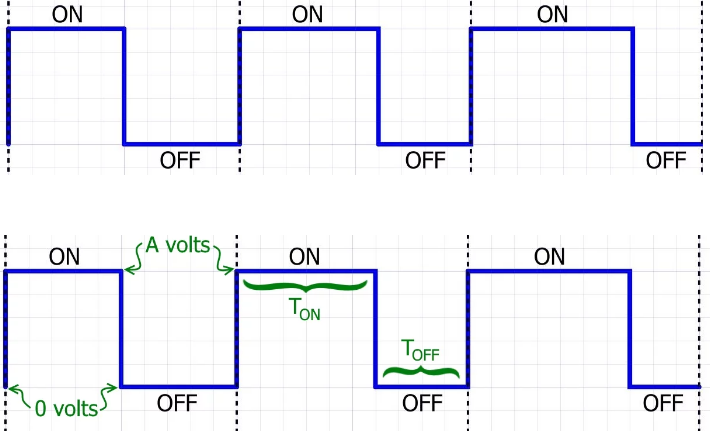
\includegraphics[width=0.7\textwidth]{PMW.png}
\end{figure}

Period of PWM has to be small enough so the effect of on/off switching be unnoticeable on load. Pulse Width (PW) determines amount of power that is fed to load.
In this experiment, period of PWM is fixed to 256~clocks and its pulse width is the value on 8-bit input of module.
\Fref{fig:PMW} shows sample PWM waves. In each cycle, first \textit{PW} clock output value is 1 and it is 0 for rest of cycle.

\begin{enumerate}
    \item Write a Verilog code for DAC module. The output of the PWM module will go to an external board with an RC low pass filter.
    \item You can use a random data input from the switches to test the accuracy of your design.
\end{enumerate}

\designverification{}

\section{Frequency Selector}

In order to set the frequency of the output signal a frequency selector (or regulated frequency) is required. The frequency selector consists of a counter that divides a high source input signal to the desired value.
You can take advantage of your previous design of the frequency regulator.
The Block diagram of this component is shown in \fref{fig:FSblockdia}.

\begin{figure}
    \centering
    \caption{Block diagram of frequency selector\label{fig:FSblockdia}}
    \resizebox{0.9\textwidth}{!}{%LaTeX with PSTricks extensions
%%Creator: inkscape 0.91
%%Please note this file requires PSTricks extensions
\psset{xunit=.5pt,yunit=.5pt,runit=.5pt}
\begin{pspicture}(617.7047309,223.22834646)
{
\newrgbcolor{curcolor}{0 0 0}
\pscustom[linewidth=0.59963652,linecolor=curcolor]
{
\newpath
\moveto(305.2149998,142.87704982)
\lineto(334.89699962,142.87704982)
}
}
{
\newrgbcolor{curcolor}{0 0 0}
\pscustom[linestyle=none,fillstyle=solid,fillcolor=curcolor]
{
\newpath
\moveto(342.39199761,142.87704982)
\lineto(335.19699726,146.47484916)
\lineto(335.19699726,139.27925048)
\lineto(342.39199761,142.87704982)
\closepath
}
}
{
\newrgbcolor{curcolor}{0 0 0}
\pscustom[linewidth=0.59963652,linecolor=curcolor]
{
\newpath
\moveto(342.39199761,142.87704982)
\lineto(335.19699726,146.47484916)
\lineto(335.19699726,139.27925048)
\lineto(342.39199761,142.87704982)
\closepath
}
}
{
\newrgbcolor{curcolor}{0 0 0}
\pscustom[linewidth=0.59963652,linecolor=curcolor]
{
\newpath
\moveto(505.7929813,142.87704982)
\lineto(542.37100078,142.87704982)
}
}
{
\newrgbcolor{curcolor}{0 0 0}
\pscustom[linestyle=none,fillstyle=solid,fillcolor=curcolor]
{
\newpath
\moveto(550.46600467,142.87704982)
\lineto(539.67298504,145.27554964)
\lineto(542.37100078,142.87704982)
\lineto(539.67298504,140.17865159)
\lineto(550.46600467,142.87704982)
\closepath
}
}
{
\newrgbcolor{curcolor}{0 0 0}
\pscustom[linewidth=0.59963652,linecolor=curcolor]
{
\newpath
\moveto(550.46600467,142.87704982)
\lineto(539.67298504,145.27554964)
\lineto(542.37100078,142.87704982)
\lineto(539.67298504,140.17865159)
\lineto(550.46600467,142.87704982)
\closepath
}
}
{
\newrgbcolor{curcolor}{1 1 1}
\pscustom[linestyle=none,fillstyle=solid,fillcolor=curcolor]
{
\newpath
\moveto(96.84129983,90.70835521)
\lineto(96.84129983,120.69035066)
\lineto(126.82299965,105.69935293)
\lineto(96.84129983,90.70835521)
\closepath
}
}
{
\newrgbcolor{curcolor}{0 0 0}
\pscustom[linewidth=0.59963652,linecolor=curcolor]
{
\newpath
\moveto(96.84129983,90.70835521)
\lineto(96.84129983,120.69035066)
\lineto(126.82299965,105.69935293)
\lineto(96.84129983,90.70835521)
\closepath
}
}
{
\newrgbcolor{curcolor}{0 0 0}
\pscustom[linewidth=0.59963652,linecolor=curcolor]
{
\newpath
\moveto(0.59963701,105.69935293)
\lineto(97.14109904,105.69935293)
}
}
{
\newrgbcolor{curcolor}{0 0 0}
\pscustom[linestyle=none,fillstyle=solid,fillcolor=curcolor]
{
\newpath
\moveto(20.57738103,119.64593256)
\lineto(21.76738344,119.34536497)
\curveto(21.51793276,118.3680091)(21.06810367,117.6217018)(20.41789617,117.10644306)
\curveto(19.77177802,116.59527367)(18.98048776,116.33968898)(18.04402538,116.33968898)
\curveto(17.07484816,116.33968898)(16.28560258,116.53597802)(15.67628863,116.92855611)
\curveto(15.07106404,117.32522355)(14.60896688,117.89773327)(14.28999716,118.64608525)
\curveto(13.9751168,119.39443723)(13.81767662,120.1979955)(13.81767662,121.05676007)
\curveto(13.81767662,121.99322238)(13.99556358,122.80904872)(14.35133749,123.50423909)
\curveto(14.71120077,124.20351881)(15.22032551,124.73309029)(15.87871172,125.09295354)
\curveto(16.54118729,125.45690614)(17.26909254,125.63888244)(18.06242748,125.63888244)
\curveto(18.96208566,125.63888244)(19.71861641,125.40987856)(20.33201971,124.95187079)
\curveto(20.94542301,124.49386302)(21.37276065,123.84978959)(21.61403261,123.01965051)
\lineto(20.4424323,122.74361904)
\curveto(20.23387518,123.39791586)(19.93126288,123.87432572)(19.53459541,124.17284864)
\curveto(19.13792794,124.47137157)(18.63902659,124.62063303)(18.03789135,124.62063303)
\curveto(17.3467903,124.62063303)(16.76814651,124.45501415)(16.30196,124.12377638)
\curveto(15.83986285,123.79253862)(15.51475909,123.34679892)(15.32664875,122.78655727)
\curveto(15.1385384,122.23040498)(15.04448323,121.65585059)(15.04448323,121.0628941)
\curveto(15.04448323,120.2981847)(15.15489582,119.62957514)(15.37572101,119.05706543)
\curveto(15.60063556,118.48864508)(15.94823076,118.06335215)(16.41850663,117.78118665)
\curveto(16.8887825,117.49902114)(17.39790724,117.35793839)(17.94588086,117.35793839)
\curveto(18.61244578,117.35793839)(19.17677682,117.55013808)(19.63887398,117.93453746)
\curveto(20.10097113,118.31893684)(20.41380682,118.88940187)(20.57738103,119.64593256)
\closepath
}
}
{
\newrgbcolor{curcolor}{0 0 0}
\pscustom[linestyle=none,fillstyle=solid,fillcolor=curcolor]
{
\newpath
\moveto(22.66295188,119.75021112)
\curveto(22.66295188,120.95657087)(22.99827902,121.85009496)(23.6689333,122.43078338)
\curveto(24.22917498,122.91332728)(24.91209733,123.15459923)(25.71770033,123.15459923)
\curveto(26.61326916,123.15459923)(27.34526376,122.86016566)(27.91368416,122.27129853)
\curveto(28.48210456,121.68652075)(28.76631475,120.87682845)(28.76631475,119.84222161)
\curveto(28.76631475,119.00390382)(28.63954474,118.34347297)(28.3860047,117.86092907)
\curveto(28.13655403,117.38247452)(27.77055672,117.01034321)(27.28801279,116.74453513)
\curveto(26.80955821,116.47872705)(26.28612073,116.34582301)(25.71770033,116.34582301)
\curveto(24.80577409,116.34582301)(24.06764544,116.6382119)(23.5033144,117.22298968)
\curveto(22.94307272,117.80776745)(22.66295188,118.6501746)(22.66295188,119.75021112)
\closepath
\moveto(23.79774799,119.75021112)
\curveto(23.79774799,118.91598268)(23.9797243,118.29031135)(24.34367693,117.87319714)
\curveto(24.70762956,117.46017227)(25.16563736,117.25365984)(25.71770033,117.25365984)
\curveto(26.26567395,117.25365984)(26.72163707,117.46221695)(27.0855897,117.87933117)
\curveto(27.44954233,118.29644539)(27.63151864,118.9323401)(27.63151864,119.78701532)
\curveto(27.63151864,120.59261827)(27.44749765,121.20193217)(27.07945567,121.61495704)
\curveto(26.71550304,122.03207126)(26.26158459,122.24062837)(25.71770033,122.24062837)
\curveto(25.16563736,122.24062837)(24.70762956,122.03411593)(24.34367693,121.62109107)
\curveto(23.9797243,121.20806621)(23.79774799,120.58443956)(23.79774799,119.75021112)
\closepath
}
}
{
\newrgbcolor{curcolor}{0 0 0}
\pscustom[linestyle=none,fillstyle=solid,fillcolor=curcolor]
{
\newpath
\moveto(34.31761463,118.87917849)
\lineto(35.40333848,118.73809574)
\curveto(35.28474717,117.98974376)(34.9800902,117.4029213)(34.48936755,116.97762837)
\curveto(34.00273427,116.5564248)(33.40364371,116.34582301)(32.69209587,116.34582301)
\curveto(31.80061641,116.34582301)(31.08293454,116.63616722)(30.53905028,117.21685564)
\curveto(29.99925537,117.80163342)(29.72935792,118.63790654)(29.72935792,119.72567499)
\curveto(29.72935792,120.42904406)(29.84590454,121.044492)(30.0789978,121.57201881)
\curveto(30.31209105,122.09954562)(30.66582029,122.49416838)(31.14018551,122.75588711)
\curveto(31.61864009,123.02169519)(32.13798822,123.15459923)(32.69822991,123.15459923)
\curveto(33.40568838,123.15459923)(33.98433217,122.9746676)(34.43416126,122.61480436)
\curveto(34.88399035,122.25903046)(35.1722899,121.75195043)(35.29905992,121.09356426)
\lineto(34.22560413,120.92794538)
\curveto(34.12337025,121.36550638)(33.94139394,121.69469946)(33.67967519,121.91552464)
\curveto(33.42204581,122.13634981)(33.10921012,122.2467624)(32.74116814,122.2467624)
\curveto(32.18501581,122.2467624)(31.73314204,122.046384)(31.38554684,121.6456272)
\curveto(31.03795163,121.24895976)(30.86415403,120.61919908)(30.86415403,119.75634515)
\curveto(30.86415403,118.88122316)(31.0318176,118.24532845)(31.36714474,117.848661)
\curveto(31.70247188,117.45199356)(32.1400329,117.25365984)(32.67982781,117.25365984)
\curveto(33.11329948,117.25365984)(33.47520743,117.38656388)(33.76555166,117.65237196)
\curveto(34.05589589,117.91818004)(34.23991688,118.32711555)(34.31761463,118.87917849)
\closepath
}
}
{
\newrgbcolor{curcolor}{0 0 0}
\pscustom[linestyle=none,fillstyle=solid,fillcolor=curcolor]
{
\newpath
\moveto(36.35411402,116.49303979)
\lineto(36.35411402,125.48553163)
\lineto(37.45823997,125.48553163)
\lineto(37.45823997,120.35748035)
\lineto(40.07133804,123.00738244)
\lineto(41.50056774,123.00738244)
\lineto(39.01015033,120.59057359)
\lineto(41.7520631,116.49303979)
\lineto(40.39030776,116.49303979)
\lineto(38.23726217,119.82381951)
\lineto(37.45823997,119.07546753)
\lineto(37.45823997,116.49303979)
\lineto(36.35411402,116.49303979)
\closepath
}
}
{
\newrgbcolor{curcolor}{0 0 0}
\pscustom[linestyle=none,fillstyle=solid,fillcolor=curcolor]
{
\newpath
\moveto(41.61097907,113.99648851)
\lineto(41.61097907,114.79391276)
\lineto(48.92888049,114.79391276)
\lineto(48.92888049,113.99648851)
\lineto(41.61097907,113.99648851)
\closepath
}
}
{
\newrgbcolor{curcolor}{0 0 0}
\pscustom[linestyle=none,fillstyle=solid,fillcolor=curcolor]
{
\newpath
\moveto(49.2907893,118.84850832)
\lineto(50.45012155,118.94665285)
\curveto(50.53599801,118.38232184)(50.73433174,117.95702891)(51.04512275,117.67077406)
\curveto(51.36000311,117.38860856)(51.73826849,117.24752581)(52.17991886,117.24752581)
\curveto(52.71153506,117.24752581)(53.16136415,117.44790421)(53.52940613,117.848661)
\curveto(53.89744812,118.2494178)(54.08146911,118.78103396)(54.08146911,119.44350949)
\curveto(54.08146911,120.07327017)(53.90358215,120.57012681)(53.54780823,120.93407942)
\curveto(53.19612367,121.29803202)(52.73402652,121.48000832)(52.16151677,121.48000832)
\curveto(51.80574285,121.48000832)(51.48472845,121.39822122)(51.19847358,121.23464702)
\curveto(50.9122187,121.07516217)(50.68730416,120.86660506)(50.52372994,120.60897569)
\lineto(49.48707836,120.74392441)
\lineto(50.35811105,125.36285097)
\lineto(54.82982114,125.36285097)
\lineto(54.82982114,124.30779736)
\lineto(51.24141181,124.30779736)
\lineto(50.7568232,121.89098851)
\curveto(51.29661811,122.26720917)(51.86299382,122.45531951)(52.45595035,122.45531951)
\curveto(53.24110658,122.45531951)(53.90358215,122.1833774)(54.44337706,121.63949317)
\curveto(54.98317196,121.09560894)(55.25306942,120.39632922)(55.25306942,119.54165401)
\curveto(55.25306942,118.72787235)(55.01588681,118.02450327)(54.54152159,117.43154679)
\curveto(53.96492248,116.70364158)(53.17772157,116.33968898)(52.17991886,116.33968898)
\curveto(51.36204779,116.33968898)(50.69343819,116.56869286)(50.17409006,117.02670063)
\curveto(49.65883128,117.4847084)(49.3643977,118.09197763)(49.2907893,118.84850832)
\closepath
}
}
{
\newrgbcolor{curcolor}{0 0 0}
\pscustom[linestyle=none,fillstyle=solid,fillcolor=curcolor]
{
\newpath
\moveto(56.28358779,120.92794538)
\curveto(56.28358779,121.99117771)(56.39195571,122.84585292)(56.60869154,123.49197102)
\curveto(56.82951673,124.14217848)(57.15462048,124.64312448)(57.58400279,124.99480902)
\curveto(58.01747446,125.34649355)(58.56135872,125.52233582)(59.21565558,125.52233582)
\curveto(59.69819952,125.52233582)(60.12144779,125.4241913)(60.48540042,125.22790226)
\curveto(60.84935305,125.03570257)(61.14992067,124.75558174)(61.38710328,124.38753979)
\curveto(61.62428589,124.02358718)(61.81035156,123.57784748)(61.94530029,123.05032067)
\curveto(62.08024901,122.52688322)(62.14772338,121.81942479)(62.14772338,120.92794538)
\curveto(62.14772338,119.87289177)(62.03935546,119.02026124)(61.82261962,118.37005378)
\curveto(61.60588379,117.72393567)(61.28078004,117.22298968)(60.84730837,116.86721578)
\curveto(60.41792606,116.51553125)(59.8740418,116.33968898)(59.21565558,116.33968898)
\curveto(58.34871225,116.33968898)(57.66783458,116.65047996)(57.17302258,117.27206194)
\curveto(56.58006605,118.02041392)(56.28358779,119.23904173)(56.28358779,120.92794538)
\closepath
\moveto(57.4183839,120.92794538)
\curveto(57.4183839,119.4516882)(57.59013683,118.4681983)(57.93364268,117.97747569)
\curveto(58.28123788,117.49084243)(58.70857552,117.24752581)(59.21565558,117.24752581)
\curveto(59.72273565,117.24752581)(60.1480286,117.49288711)(60.49153446,117.98360972)
\curveto(60.83912966,118.47433233)(61.01292726,119.45577755)(61.01292726,120.92794538)
\curveto(61.01292726,122.40829192)(60.83912966,123.39178182)(60.49153446,123.87841508)
\curveto(60.1480286,124.36504833)(59.71864629,124.60836496)(59.20338752,124.60836496)
\curveto(58.69630745,124.60836496)(58.29146127,124.39367382)(57.98884897,123.96429153)
\curveto(57.60853893,123.41631795)(57.4183839,122.40420257)(57.4183839,120.92794538)
\closepath
}
}
{
\newrgbcolor{curcolor}{1 1 1}
\pscustom[linestyle=none,fillstyle=solid,fillcolor=curcolor]
{
\newpath
\moveto(141.51400075,172.55904765)
\lineto(141.51400075,113.19535317)
\lineto(305.2149998,113.19535317)
\lineto(305.2149998,172.55904765)
\lineto(141.51400075,172.55904765)
\closepath
}
}
{
\newrgbcolor{curcolor}{0 0 0}
\pscustom[linewidth=0.59963652,linecolor=curcolor]
{
\newpath
\moveto(141.51400075,172.55904765)
\lineto(305.2149998,172.55904765)
\lineto(305.2149998,113.19535317)
\lineto(141.51400075,113.19535317)
\closepath
}
}
{
\newrgbcolor{curcolor}{1 1 1}
\pscustom[linestyle=none,fillstyle=solid,fillcolor=curcolor]
{
\newpath
\moveto(211.22199798,157.73675031)
\lineto(211.22199798,143.77655015)
\lineto(235.52599823,143.77655015)
\lineto(235.52599823,157.73675031)
\lineto(211.22199798,157.73675031)
\closepath
}
}
{
\newrgbcolor{curcolor}{0 0 0}
\pscustom[linestyle=none,fillstyle=solid,fillcolor=curcolor]
{
\newpath
\moveto(212.5918143,146.47486628)
\lineto(212.5918143,155.46735811)
\lineto(213.78181671,155.46735811)
\lineto(213.78181671,147.53605392)
\lineto(218.21058857,147.53605392)
\lineto(218.21058857,146.47486628)
\lineto(212.5918143,146.47486628)
\closepath
}
}
{
\newrgbcolor{curcolor}{0 0 0}
\pscustom[linestyle=none,fillstyle=solid,fillcolor=curcolor]
{
\newpath
\moveto(219.20430194,149.36399564)
\lineto(220.32682998,149.46214017)
\curveto(220.3799916,149.01231111)(220.50267226,148.64222447)(220.69487197,148.35188026)
\curveto(220.89116102,148.0656254)(221.19377332,147.83253216)(221.60270886,147.65260054)
\curveto(222.01164439,147.47675827)(222.47169687,147.38883714)(222.98286629,147.38883714)
\curveto(223.43678474,147.38883714)(223.83754156,147.4563115)(224.18513677,147.59126021)
\curveto(224.53273197,147.72620893)(224.79036136,147.91022991)(224.95802493,148.14332315)
\curveto(225.12977786,148.38050575)(225.21565432,148.63813512)(225.21565432,148.91621126)
\curveto(225.21565432,149.19837676)(225.13386721,149.44373807)(224.970293,149.65229518)
\curveto(224.80671878,149.86494164)(224.53682133,150.04282859)(224.16060063,150.18595602)
\curveto(223.91932867,150.28001118)(223.38566779,150.42518329)(222.55961801,150.62147233)
\curveto(221.73356823,150.82185073)(221.15492444,151.00996107)(220.82368666,151.18580333)
\curveto(220.39430435,151.41071786)(220.07328995,151.68879401)(219.86064347,152.02003177)
\curveto(219.65208635,152.35535889)(219.54780779,152.72953488)(219.54780779,153.14255974)
\curveto(219.54780779,153.59647816)(219.67662248,154.01972641)(219.93425187,154.4123045)
\curveto(220.19188126,154.80897194)(220.56810195,155.10953954)(221.06291395,155.31400729)
\curveto(221.55772595,155.51847505)(222.10774424,155.62070892)(222.71296884,155.62070892)
\curveto(223.37953376,155.62070892)(223.96635626,155.51234102)(224.47343632,155.2956052)
\curveto(224.98460574,155.08295873)(225.37718385,154.76807839)(225.65117066,154.35096417)
\curveto(225.92515747,153.93384995)(226.07237427,153.46152944)(226.09282104,152.93400263)
\lineto(224.9518909,152.84812618)
\curveto(224.89055057,153.41654653)(224.68199344,153.84592882)(224.32621953,154.13627303)
\curveto(223.97453497,154.42661724)(223.45314216,154.57178935)(222.7620411,154.57178935)
\curveto(222.04231456,154.57178935)(221.51683239,154.43888531)(221.18559461,154.17307722)
\curveto(220.85844618,153.9113585)(220.69487197,153.59443348)(220.69487197,153.22230217)
\curveto(220.69487197,152.89924312)(220.81141859,152.63343503)(221.04451185,152.42487793)
\curveto(221.27351575,152.21632082)(221.87056163,152.00162967)(222.8356495,151.7808045)
\curveto(223.80482672,151.56406868)(224.46934696,151.37391367)(224.82921024,151.21033947)
\curveto(225.35264772,150.96906752)(225.7390918,150.66236588)(225.98854248,150.29023457)
\curveto(226.23799316,149.92219261)(226.3627185,149.49689968)(226.3627185,149.01435578)
\curveto(226.3627185,148.53590124)(226.22572509,148.0840275)(225.95173828,147.65873457)
\curveto(225.67775147,147.237531)(225.28312868,146.90833792)(224.76786991,146.67115532)
\curveto(224.25670049,146.43806208)(223.68010138,146.32151546)(223.03807259,146.32151546)
\curveto(222.22429087,146.32151546)(221.54136853,146.44010676)(220.98930555,146.67728935)
\curveto(220.44133193,146.91447195)(220.00990494,147.27024584)(219.69502458,147.74461103)
\curveto(219.38423357,148.22306558)(219.22065936,148.76286045)(219.20430194,149.36399564)
\closepath
}
}
{
\newrgbcolor{curcolor}{0 0 0}
\pscustom[linestyle=none,fillstyle=solid,fillcolor=curcolor]
{
\newpath
\moveto(227.92689609,146.47486628)
\lineto(227.92689609,155.46735811)
\lineto(231.30061426,155.46735811)
\curveto(231.98762597,155.46735811)(232.53764426,155.37534762)(232.95066915,155.19132664)
\curveto(233.3677834,155.01139502)(233.69288715,154.73127419)(233.92598041,154.35096417)
\curveto(234.16316302,153.9747435)(234.28175432,153.58012074)(234.28175432,153.16709587)
\curveto(234.28175432,152.7826965)(234.17747576,152.42078857)(233.96891864,152.0813721)
\curveto(233.76036151,151.74195563)(233.44548115,151.46796884)(233.02427755,151.25941173)
\curveto(233.56816181,151.09992688)(233.98527606,150.82798476)(234.27562029,150.44358539)
\curveto(234.57005388,150.05918601)(234.71727067,149.60526759)(234.71727067,149.08183014)
\curveto(234.71727067,148.66062657)(234.62730485,148.26804848)(234.44737321,147.90409588)
\curveto(234.27153093,147.54423263)(234.05275042,147.26615649)(233.79103168,147.06986744)
\curveto(233.52931294,146.8735784)(233.20011983,146.72431694)(232.80345236,146.62208306)
\curveto(232.41087424,146.52393854)(231.92833031,146.47486628)(231.35582056,146.47486628)
\lineto(227.92689609,146.47486628)
\closepath
\moveto(229.1168985,151.68879401)
\lineto(231.06138698,151.68879401)
\curveto(231.58891382,151.68879401)(231.96717919,151.72355353)(232.19618309,151.79307256)
\curveto(232.49879539,151.88303838)(232.72575461,152.03229984)(232.87706076,152.24085695)
\curveto(233.03245626,152.44941406)(233.11015401,152.71113278)(233.11015401,153.02601312)
\curveto(233.11015401,153.32453604)(233.03859029,153.58625477)(232.89546286,153.8111693)
\curveto(232.75233542,154.04017318)(232.54786765,154.19556868)(232.28205955,154.27735578)
\curveto(232.01625145,154.36323224)(231.56028833,154.40617046)(230.91417018,154.40617046)
\lineto(229.1168985,154.40617046)
\lineto(229.1168985,151.68879401)
\closepath
\moveto(229.1168985,147.53605392)
\lineto(231.35582056,147.53605392)
\curveto(231.74021997,147.53605392)(232.01011742,147.55036666)(232.16551292,147.57899215)
\curveto(232.43949973,147.62806441)(232.66850363,147.70985151)(232.85252462,147.82435345)
\curveto(233.03654562,147.9388554)(233.18785176,148.10447428)(233.30644307,148.3212101)
\curveto(233.42503437,148.54203527)(233.48433003,148.79557529)(233.48433003,149.08183014)
\curveto(233.48433003,149.41715726)(233.39845356,149.70750147)(233.22670064,149.95286278)
\curveto(233.05494771,150.20231344)(232.81572043,150.37611103)(232.50901877,150.47425555)
\curveto(232.20640648,150.57648943)(231.76884545,150.62760637)(231.1963357,150.62760637)
\lineto(229.1168985,150.62760637)
\lineto(229.1168985,147.53605392)
\closepath
}
}
{
\newrgbcolor{curcolor}{1 1 1}
\pscustom[linestyle=none,fillstyle=solid,fillcolor=curcolor]
{
\newpath
\moveto(200.50299804,142.87704982)
\lineto(200.50299804,128.91675045)
\lineto(246.24499817,128.91675045)
\lineto(246.24499817,142.87704982)
\lineto(200.50299804,142.87704982)
\closepath
}
}
{
\newrgbcolor{curcolor}{0 0 0}
\pscustom[linestyle=none,fillstyle=solid,fillcolor=curcolor]
{
\newpath
\moveto(208.56343873,134.63684919)
\lineto(209.75344114,134.33628159)
\curveto(209.50399046,133.35892572)(209.05416137,132.61261842)(208.40395387,132.09735968)
\curveto(207.75783572,131.58619029)(206.96654546,131.3306056)(206.03008308,131.3306056)
\curveto(205.06090586,131.3306056)(204.27166028,131.52689464)(203.66234633,131.91947273)
\curveto(203.05712174,132.31614017)(202.59502458,132.88864989)(202.27605486,133.63700187)
\curveto(201.9611745,134.38535385)(201.80373432,135.18891212)(201.80373432,136.04767669)
\curveto(201.80373432,136.984139)(201.98162128,137.79996534)(202.33739519,138.49515571)
\curveto(202.69725847,139.19443543)(203.20638321,139.72400691)(203.86476942,140.08387016)
\curveto(204.52724499,140.44782276)(205.25515024,140.62979906)(206.04848518,140.62979906)
\curveto(206.94814336,140.62979906)(207.7046741,140.40079518)(208.31807741,139.94278741)
\curveto(208.93148071,139.48477964)(209.35881835,138.84070621)(209.60009031,138.01056713)
\lineto(208.42849,137.73453566)
\curveto(208.21993288,138.38883248)(207.91732058,138.86524234)(207.52065311,139.16376526)
\curveto(207.12398564,139.46228819)(206.62508429,139.61154965)(206.02394905,139.61154965)
\curveto(205.33284799,139.61154965)(204.75420421,139.44593077)(204.2880177,139.114693)
\curveto(203.82592054,138.78345524)(203.50081679,138.33771554)(203.31270645,137.77747389)
\curveto(203.1245961,137.2213216)(203.03054093,136.64676721)(203.03054093,136.05381072)
\curveto(203.03054093,135.28910132)(203.14095352,134.62049176)(203.36177871,134.04798205)
\curveto(203.58669326,133.4795617)(203.93428846,133.05426877)(204.40456433,132.77210327)
\curveto(204.87484019,132.48993777)(205.38396494,132.34885501)(205.93193856,132.34885501)
\curveto(206.59850348,132.34885501)(207.16283452,132.5410547)(207.62493167,132.92545408)
\curveto(208.08702883,133.30985346)(208.39986452,133.88031849)(208.56343873,134.63684919)
\closepath
}
}
{
\newrgbcolor{curcolor}{0 0 0}
\pscustom[linestyle=none,fillstyle=solid,fillcolor=curcolor]
{
\newpath
\moveto(210.64900958,134.74112774)
\curveto(210.64900958,135.94748749)(210.98433672,136.84101158)(211.65499099,137.4217)
\curveto(212.21523268,137.9042439)(212.89815502,138.14551585)(213.70375803,138.14551585)
\curveto(214.59932685,138.14551585)(215.33132146,137.85108228)(215.89974186,137.26221515)
\curveto(216.46816225,136.67743737)(216.75237245,135.86774507)(216.75237245,134.83313823)
\curveto(216.75237245,133.99482044)(216.62560244,133.33438959)(216.3720624,132.85184569)
\curveto(216.12261173,132.37339115)(215.75661442,132.00125983)(215.27407049,131.73545175)
\curveto(214.79561591,131.46964367)(214.27217843,131.33673963)(213.70375803,131.33673963)
\curveto(212.79183178,131.33673963)(212.05370314,131.62912852)(211.4893721,132.2139063)
\curveto(210.92913042,132.79868407)(210.64900958,133.64109122)(210.64900958,134.74112774)
\closepath
\moveto(211.78380569,134.74112774)
\curveto(211.78380569,133.9068993)(211.965782,133.28122797)(212.32973463,132.86411376)
\curveto(212.69368726,132.45108889)(213.15169506,132.24457646)(213.70375803,132.24457646)
\curveto(214.25173165,132.24457646)(214.70769477,132.45313357)(215.0716474,132.87024779)
\curveto(215.43560003,133.28736201)(215.61757634,133.92325672)(215.61757634,134.77793194)
\curveto(215.61757634,135.58353489)(215.43355535,136.1928488)(215.06551337,136.60587366)
\curveto(214.70156074,137.02298788)(214.24764229,137.23154499)(213.70375803,137.23154499)
\curveto(213.15169506,137.23154499)(212.69368726,137.02503255)(212.32973463,136.61200769)
\curveto(211.965782,136.19898283)(211.78380569,135.57535618)(211.78380569,134.74112774)
\closepath
}
}
{
\newrgbcolor{curcolor}{0 0 0}
\pscustom[linestyle=none,fillstyle=solid,fillcolor=curcolor]
{
\newpath
\moveto(222.32207443,131.48395641)
\lineto(222.32207443,132.4408655)
\curveto(221.81499436,131.70478159)(221.12593799,131.33673963)(220.25490529,131.33673963)
\curveto(219.87050589,131.33673963)(219.51064262,131.41034802)(219.17531548,131.55756481)
\curveto(218.84407769,131.70478159)(218.59667169,131.88880257)(218.43309748,132.10962774)
\curveto(218.27361262,132.33454227)(218.16115535,132.60852906)(218.09572566,132.93158811)
\curveto(218.05074275,133.14832393)(218.0282513,133.49182976)(218.0282513,133.9621056)
\lineto(218.0282513,137.99829907)
\lineto(219.13237725,137.99829907)
\lineto(219.13237725,134.38535385)
\curveto(219.13237725,133.80875478)(219.1548687,133.42026605)(219.19985161,133.21988765)
\curveto(219.26937065,132.92954344)(219.41658744,132.70053955)(219.64150199,132.53287599)
\curveto(219.86641653,132.36930179)(220.1444927,132.28751469)(220.47573048,132.28751469)
\curveto(220.80696827,132.28751469)(221.11775927,132.37134647)(221.4081035,132.53901003)
\curveto(221.69844774,132.71076294)(221.9029155,132.9418115)(222.02150681,133.23215571)
\curveto(222.14418747,133.52658928)(222.2055278,133.95188221)(222.2055278,134.5080345)
\lineto(222.2055278,137.99829907)
\lineto(223.30965375,137.99829907)
\lineto(223.30965375,131.48395641)
\lineto(222.32207443,131.48395641)
\closepath
}
}
{
\newrgbcolor{curcolor}{0 0 0}
\pscustom[linestyle=none,fillstyle=solid,fillcolor=curcolor]
{
\newpath
\moveto(225.04558423,131.48395641)
\lineto(225.04558423,137.99829907)
\lineto(226.03929758,137.99829907)
\lineto(226.03929758,137.07206014)
\curveto(226.51775216,137.78769728)(227.20885321,138.14551585)(228.11260075,138.14551585)
\curveto(228.50517886,138.14551585)(228.86504214,138.07395213)(229.19219056,137.93082471)
\curveto(229.52342835,137.79178663)(229.77083435,137.60776565)(229.93440856,137.37876177)
\curveto(230.09798278,137.14975789)(230.21248473,136.87781577)(230.27791441,136.56293543)
\curveto(230.31880797,136.35846768)(230.33925474,136.00064911)(230.33925474,135.48947972)
\lineto(230.33925474,131.48395641)
\lineto(229.2351288,131.48395641)
\lineto(229.2351288,135.44654149)
\curveto(229.2351288,135.89637055)(229.19219056,136.23169767)(229.1063141,136.45252284)
\curveto(229.02043764,136.67743737)(228.86708681,136.85532432)(228.64626162,136.98618368)
\curveto(228.42952579,137.1211324)(228.17394108,137.18860676)(227.87950749,137.18860676)
\curveto(227.40923163,137.18860676)(227.00234077,137.0393453)(226.65883492,136.74082238)
\curveto(226.31941842,136.44229946)(226.14971018,135.87592378)(226.14971018,135.04169534)
\lineto(226.14971018,131.48395641)
\lineto(225.04558423,131.48395641)
\closepath
}
}
{
\newrgbcolor{curcolor}{0 0 0}
\pscustom[linestyle=none,fillstyle=solid,fillcolor=curcolor]
{
\newpath
\moveto(234.4490577,132.47153567)
\lineto(234.60854256,131.49622448)
\curveto(234.29775155,131.4307948)(234.01967539,131.39807996)(233.77431407,131.39807996)
\curveto(233.37355724,131.39807996)(233.06276623,131.46146496)(232.84194104,131.58823497)
\curveto(232.62111585,131.71500498)(232.46572035,131.88062386)(232.37575453,132.08509161)
\curveto(232.28578871,132.29364872)(232.24080581,132.72916504)(232.24080581,133.39164056)
\lineto(232.24080581,137.1395345)
\lineto(231.43111344,137.1395345)
\lineto(231.43111344,137.99829907)
\lineto(232.24080581,137.99829907)
\lineto(232.24080581,139.61154965)
\lineto(233.33879772,140.27402517)
\lineto(233.33879772,137.99829907)
\lineto(234.4490577,137.99829907)
\lineto(234.4490577,137.1395345)
\lineto(233.33879772,137.1395345)
\lineto(233.33879772,133.33030024)
\curveto(233.33879772,133.01541989)(233.35719982,132.81299682)(233.39400402,132.72303101)
\curveto(233.43489757,132.63306519)(233.49828258,132.56150148)(233.58415904,132.50833986)
\curveto(233.67412486,132.45517825)(233.80089488,132.42859744)(233.96446909,132.42859744)
\curveto(234.08714975,132.42859744)(234.24867929,132.44291018)(234.4490577,132.47153567)
\closepath
}
}
{
\newrgbcolor{curcolor}{0 0 0}
\pscustom[linestyle=none,fillstyle=solid,fillcolor=curcolor]
{
\newpath
\moveto(239.98195594,133.58179557)
\lineto(241.12288608,133.44071282)
\curveto(240.94295445,132.77414794)(240.60967198,132.25684453)(240.1230387,131.88880257)
\curveto(239.63640541,131.52076061)(239.01482339,131.33673963)(238.25829265,131.33673963)
\curveto(237.30547285,131.33673963)(236.54894211,131.62912852)(235.98870043,132.2139063)
\curveto(235.4325481,132.80277343)(235.15447193,133.62677848)(235.15447193,134.68592145)
\curveto(235.15447193,135.78186861)(235.43663745,136.63245447)(236.00096849,137.23767902)
\curveto(236.56529953,137.84290357)(237.29729414,138.14551585)(238.19695232,138.14551585)
\curveto(239.06798501,138.14551585)(239.77953285,137.8490376)(240.33159582,137.25608112)
\curveto(240.88365879,136.66312463)(241.15969028,135.82889619)(241.15969028,134.75339581)
\curveto(241.15969028,134.68796612)(241.1576456,134.5898216)(241.15355625,134.45896224)
\lineto(236.29540208,134.45896224)
\curveto(236.33629563,133.7433251)(236.53871872,133.19535152)(236.90267135,132.81504149)
\curveto(237.26662398,132.43473147)(237.72054242,132.24457646)(238.26442668,132.24457646)
\curveto(238.66927286,132.24457646)(239.01482339,132.35089969)(239.30107827,132.56354616)
\curveto(239.58733314,132.77619262)(239.81429237,133.11560909)(239.98195594,133.58179557)
\closepath
\moveto(236.35674241,135.36679907)
\lineto(239.994224,135.36679907)
\curveto(239.94515174,135.91477265)(239.80611365,136.32575284)(239.57710975,136.59973963)
\curveto(239.22542519,137.02503255)(238.76946207,137.23767902)(238.20922039,137.23767902)
\curveto(237.70214032,137.23767902)(237.27480269,137.06797078)(236.92720748,136.72855431)
\curveto(236.58370163,136.38913784)(236.39354661,135.93521942)(236.35674241,135.36679907)
\closepath
}
}
{
\newrgbcolor{curcolor}{0 0 0}
\pscustom[linestyle=none,fillstyle=solid,fillcolor=curcolor]
{
\newpath
\moveto(242.50304434,131.48395641)
\lineto(242.50304434,137.99829907)
\lineto(243.49675769,137.99829907)
\lineto(243.49675769,137.01071981)
\curveto(243.75029772,137.47281694)(243.98339098,137.77747389)(244.19603745,137.92469067)
\curveto(244.41277329,138.07190746)(244.6499559,138.14551585)(244.90758529,138.14551585)
\curveto(245.27971663,138.14551585)(245.657982,138.02692455)(246.0423814,137.78974196)
\lineto(245.66207135,136.76535851)
\curveto(245.3921739,136.92484336)(245.12227644,137.00458578)(244.85237899,137.00458578)
\curveto(244.61110702,137.00458578)(244.39437119,136.93097739)(244.20217149,136.7837606)
\curveto(244.00997179,136.64063318)(243.87297838,136.44025478)(243.79119127,136.18262541)
\curveto(243.66851061,135.79004732)(243.60717028,135.36066504)(243.60717028,134.89447856)
\lineto(243.60717028,131.48395641)
\lineto(242.50304434,131.48395641)
\closepath
}
}
{
\newrgbcolor{curcolor}{1 1 1}
\pscustom[linestyle=none,fillstyle=solid,fillcolor=curcolor]
{
\newpath
\moveto(342.39199761,172.55904765)
\lineto(342.39199761,113.19535317)
\lineto(506.09299311,113.19535317)
\lineto(506.09299311,172.55904765)
\lineto(342.39199761,172.55904765)
\closepath
}
}
{
\newrgbcolor{curcolor}{0 0 0}
\pscustom[linewidth=0.59963652,linecolor=curcolor]
{
\newpath
\moveto(342.39199761,172.55904765)
\lineto(506.09299311,172.55904765)
\lineto(506.09299311,113.19535317)
\lineto(342.39199761,113.19535317)
\closepath
}
}
{
\newrgbcolor{curcolor}{1 1 1}
\pscustom[linestyle=none,fillstyle=solid,fillcolor=curcolor]
{
\newpath
\moveto(410.31998973,157.73675031)
\lineto(410.31998973,143.77655015)
\lineto(438.18398957,143.77655015)
\lineto(438.18398957,157.73675031)
\lineto(410.31998973,157.73675031)
\closepath
}
}
{
\newrgbcolor{curcolor}{0 0 0}
\pscustom[linestyle=none,fillstyle=solid,fillcolor=curcolor]
{
\newpath
\moveto(411.68344307,146.47486628)
\lineto(411.68344307,155.46735811)
\lineto(413.47458072,155.46735811)
\lineto(415.60309018,149.10023224)
\curveto(415.79937924,148.50727575)(415.94250668,148.06358073)(416.03247249,147.76914716)
\curveto(416.13470638,148.09629557)(416.29419124,148.57679479)(416.51092707,149.21064483)
\lineto(418.66397267,155.46735811)
\lineto(420.26495529,155.46735811)
\lineto(420.26495529,146.47486628)
\lineto(419.11789111,146.47486628)
\lineto(419.11789111,154.00132431)
\lineto(416.50479304,146.47486628)
\lineto(415.43133726,146.47486628)
\lineto(412.83050725,154.130139)
\lineto(412.83050725,146.47486628)
\lineto(411.68344307,146.47486628)
\closepath
}
}
{
\newrgbcolor{curcolor}{0 0 0}
\pscustom[linestyle=none,fillstyle=solid,fillcolor=curcolor]
{
\newpath
\moveto(421.767793,149.36399564)
\lineto(422.89032104,149.46214017)
\curveto(422.94348266,149.01231111)(423.06616332,148.64222447)(423.25836302,148.35188026)
\curveto(423.45465208,148.0656254)(423.75726438,147.83253216)(424.16619991,147.65260054)
\curveto(424.57513545,147.47675827)(425.03518793,147.38883714)(425.54635735,147.38883714)
\curveto(426.00027579,147.38883714)(426.40103262,147.4563115)(426.74862782,147.59126021)
\curveto(427.09622303,147.72620893)(427.35385242,147.91022991)(427.52151599,148.14332315)
\curveto(427.69326891,148.38050575)(427.77914538,148.63813512)(427.77914538,148.91621126)
\curveto(427.77914538,149.19837676)(427.69735827,149.44373807)(427.53378405,149.65229518)
\curveto(427.37020984,149.86494164)(427.10031239,150.04282859)(426.72409169,150.18595602)
\curveto(426.48281973,150.28001118)(425.94915885,150.42518329)(425.12310907,150.62147233)
\curveto(424.29705929,150.82185073)(423.7184155,151.00996107)(423.38717772,151.18580333)
\curveto(422.95779541,151.41071786)(422.63678101,151.68879401)(422.42413453,152.02003177)
\curveto(422.21557741,152.35535889)(422.11129885,152.72953488)(422.11129885,153.14255974)
\curveto(422.11129885,153.59647816)(422.24011354,154.01972641)(422.49774293,154.4123045)
\curveto(422.75537232,154.80897194)(423.13159301,155.10953954)(423.62640501,155.31400729)
\curveto(424.12121701,155.51847505)(424.6712353,155.62070892)(425.27645989,155.62070892)
\curveto(425.94302482,155.62070892)(426.52984731,155.51234102)(427.03692738,155.2956052)
\curveto(427.5480968,155.08295873)(427.94067491,154.76807839)(428.21466172,154.35096417)
\curveto(428.48864853,153.93384995)(428.63586532,153.46152944)(428.6563121,152.93400263)
\lineto(427.51538195,152.84812618)
\curveto(427.45404162,153.41654653)(427.2454845,153.84592882)(426.88971058,154.13627303)
\curveto(426.53802602,154.42661724)(426.01663322,154.57178935)(425.32553216,154.57178935)
\curveto(424.60580562,154.57178935)(424.08032345,154.43888531)(423.74908567,154.17307722)
\curveto(423.42193724,153.9113585)(423.25836302,153.59443348)(423.25836302,153.22230217)
\curveto(423.25836302,152.89924312)(423.37490965,152.63343503)(423.60800291,152.42487793)
\curveto(423.83700681,152.21632082)(424.43405269,152.00162967)(425.39914056,151.7808045)
\curveto(426.36831778,151.56406868)(427.03283802,151.37391367)(427.39270129,151.21033947)
\curveto(427.91613878,150.96906752)(428.30258286,150.66236588)(428.55203354,150.29023457)
\curveto(428.80148422,149.92219261)(428.92620955,149.49689968)(428.92620955,149.01435578)
\curveto(428.92620955,148.53590124)(428.78921615,148.0840275)(428.51522934,147.65873457)
\curveto(428.24124253,147.237531)(427.84661974,146.90833792)(427.33136096,146.67115532)
\curveto(426.82019154,146.43806208)(426.24359244,146.32151546)(425.60156365,146.32151546)
\curveto(424.78778193,146.32151546)(424.10485958,146.44010676)(423.55279661,146.67728935)
\curveto(423.00482299,146.91447195)(422.573396,147.27024584)(422.25851564,147.74461103)
\curveto(421.94772463,148.22306558)(421.78415042,148.76286045)(421.767793,149.36399564)
\closepath
}
}
{
\newrgbcolor{curcolor}{0 0 0}
\pscustom[linestyle=none,fillstyle=solid,fillcolor=curcolor]
{
\newpath
\moveto(430.49038799,146.47486628)
\lineto(430.49038799,155.46735811)
\lineto(433.86410617,155.46735811)
\curveto(434.55111787,155.46735811)(435.10113616,155.37534762)(435.51416105,155.19132664)
\curveto(435.9312753,155.01139502)(436.25637905,154.73127419)(436.48947231,154.35096417)
\curveto(436.72665492,153.9747435)(436.84524622,153.58012074)(436.84524622,153.16709587)
\curveto(436.84524622,152.7826965)(436.74096766,152.42078857)(436.53241054,152.0813721)
\curveto(436.32385342,151.74195563)(436.00897305,151.46796884)(435.58776945,151.25941173)
\curveto(436.13165371,151.09992688)(436.54876796,150.82798476)(436.83911219,150.44358539)
\curveto(437.13354578,150.05918601)(437.28076257,149.60526759)(437.28076257,149.08183014)
\curveto(437.28076257,148.66062657)(437.19079675,148.26804848)(437.01086512,147.90409588)
\curveto(436.83502284,147.54423263)(436.61624232,147.26615649)(436.35452358,147.06986744)
\curveto(436.09280484,146.8735784)(435.76361173,146.72431694)(435.36694426,146.62208306)
\curveto(434.97436615,146.52393854)(434.49182221,146.47486628)(433.91931246,146.47486628)
\lineto(430.49038799,146.47486628)
\closepath
\moveto(431.6803904,151.68879401)
\lineto(433.62487888,151.68879401)
\curveto(434.15240572,151.68879401)(434.53067109,151.72355353)(434.75967499,151.79307256)
\curveto(435.06228729,151.88303838)(435.28924651,152.03229984)(435.44055266,152.24085695)
\curveto(435.59594816,152.44941406)(435.67364591,152.71113278)(435.67364591,153.02601312)
\curveto(435.67364591,153.32453604)(435.6020822,153.58625477)(435.45895476,153.8111693)
\curveto(435.31582732,154.04017318)(435.11135955,154.19556868)(434.84555145,154.27735578)
\curveto(434.57974335,154.36323224)(434.12378023,154.40617046)(433.47766209,154.40617046)
\lineto(431.6803904,154.40617046)
\lineto(431.6803904,151.68879401)
\closepath
\moveto(431.6803904,147.53605392)
\lineto(433.91931246,147.53605392)
\curveto(434.30371187,147.53605392)(434.57360932,147.55036666)(434.72900483,147.57899215)
\curveto(435.00299163,147.62806441)(435.23199553,147.70985151)(435.41601653,147.82435345)
\curveto(435.60003752,147.9388554)(435.75134367,148.10447428)(435.86993497,148.3212101)
\curveto(435.98852628,148.54203527)(436.04782193,148.79557529)(436.04782193,149.08183014)
\curveto(436.04782193,149.41715726)(435.96194547,149.70750147)(435.79019254,149.95286278)
\curveto(435.61843962,150.20231344)(435.37921233,150.37611103)(435.07251068,150.47425555)
\curveto(434.76989838,150.57648943)(434.33233736,150.62760637)(433.75982761,150.62760637)
\lineto(431.6803904,150.62760637)
\lineto(431.6803904,147.53605392)
\closepath
}
}
{
\newrgbcolor{curcolor}{1 1 1}
\pscustom[linestyle=none,fillstyle=solid,fillcolor=curcolor]
{
\newpath
\moveto(401.38199766,142.87704982)
\lineto(401.38199766,128.91675045)
\lineto(447.12300921,128.91675045)
\lineto(447.12300921,142.87704982)
\lineto(401.38199766,142.87704982)
\closepath
}
}
{
\newrgbcolor{curcolor}{0 0 0}
\pscustom[linestyle=none,fillstyle=solid,fillcolor=curcolor]
{
\newpath
\moveto(409.44170252,134.63684919)
\lineto(410.63170493,134.33628159)
\curveto(410.38225425,133.35892572)(409.93242516,132.61261842)(409.28221766,132.09735968)
\curveto(408.63609951,131.58619029)(407.84480925,131.3306056)(406.90834687,131.3306056)
\curveto(405.93916965,131.3306056)(405.14992407,131.52689464)(404.54061012,131.91947273)
\curveto(403.93538553,132.31614017)(403.47328837,132.88864989)(403.15431865,133.63700187)
\curveto(402.83943829,134.38535385)(402.68199811,135.18891212)(402.68199811,136.04767669)
\curveto(402.68199811,136.984139)(402.85988507,137.79996534)(403.21565898,138.49515571)
\curveto(403.57552225,139.19443543)(404.084647,139.72400691)(404.74303321,140.08387016)
\curveto(405.40550878,140.44782276)(406.13341403,140.62979906)(406.92674897,140.62979906)
\curveto(407.82640715,140.62979906)(408.58293789,140.40079518)(409.1963412,139.94278741)
\curveto(409.8097445,139.48477964)(410.23708214,138.84070621)(410.4783541,138.01056713)
\lineto(409.30675379,137.73453566)
\curveto(409.09819667,138.38883248)(408.79558437,138.86524234)(408.3989169,139.16376526)
\curveto(408.00224943,139.46228819)(407.50334808,139.61154965)(406.90221284,139.61154965)
\curveto(406.21111178,139.61154965)(405.632468,139.44593077)(405.16628149,139.114693)
\curveto(404.70418433,138.78345524)(404.37908058,138.33771554)(404.19097024,137.77747389)
\curveto(404.00285989,137.2213216)(403.90880472,136.64676721)(403.90880472,136.05381072)
\curveto(403.90880472,135.28910132)(404.01921731,134.62049176)(404.2400425,134.04798205)
\curveto(404.46495705,133.4795617)(404.81255225,133.05426877)(405.28282812,132.77210327)
\curveto(405.75310398,132.48993777)(406.26222873,132.34885501)(406.81020234,132.34885501)
\curveto(407.47676727,132.34885501)(408.04109831,132.5410547)(408.50319546,132.92545408)
\curveto(408.96529262,133.30985346)(409.2781283,133.88031849)(409.44170252,134.63684919)
\closepath
}
}
{
\newrgbcolor{curcolor}{0 0 0}
\pscustom[linestyle=none,fillstyle=solid,fillcolor=curcolor]
{
\newpath
\moveto(411.52727337,134.74112774)
\curveto(411.52727337,135.94748749)(411.86260051,136.84101158)(412.53325478,137.4217)
\curveto(413.09349647,137.9042439)(413.77641881,138.14551585)(414.58202182,138.14551585)
\curveto(415.47759064,138.14551585)(416.20958525,137.85108228)(416.77800565,137.26221515)
\curveto(417.34642604,136.67743737)(417.63063624,135.86774507)(417.63063624,134.83313823)
\curveto(417.63063624,133.99482044)(417.50386623,133.33438959)(417.25032619,132.85184569)
\curveto(417.00087552,132.37339115)(416.63487821,132.00125983)(416.15233428,131.73545175)
\curveto(415.6738797,131.46964367)(415.15044222,131.33673963)(414.58202182,131.33673963)
\curveto(413.67009557,131.33673963)(412.93196693,131.62912852)(412.36763589,132.2139063)
\curveto(411.80739421,132.79868407)(411.52727337,133.64109122)(411.52727337,134.74112774)
\closepath
\moveto(412.66206948,134.74112774)
\curveto(412.66206948,133.9068993)(412.84404579,133.28122797)(413.20799842,132.86411376)
\curveto(413.57195105,132.45108889)(414.02995885,132.24457646)(414.58202182,132.24457646)
\curveto(415.12999544,132.24457646)(415.58595856,132.45313357)(415.94991119,132.87024779)
\curveto(416.31386382,133.28736201)(416.49584013,133.92325672)(416.49584013,134.77793194)
\curveto(416.49584013,135.58353489)(416.31181914,136.1928488)(415.94377715,136.60587366)
\curveto(415.57982453,137.02298788)(415.12590608,137.23154499)(414.58202182,137.23154499)
\curveto(414.02995885,137.23154499)(413.57195105,137.02503255)(413.20799842,136.61200769)
\curveto(412.84404579,136.19898283)(412.66206948,135.57535618)(412.66206948,134.74112774)
\closepath
}
}
{
\newrgbcolor{curcolor}{0 0 0}
\pscustom[linestyle=none,fillstyle=solid,fillcolor=curcolor]
{
\newpath
\moveto(423.20033822,131.48395641)
\lineto(423.20033822,132.4408655)
\curveto(422.69325815,131.70478159)(422.00420177,131.33673963)(421.13316908,131.33673963)
\curveto(420.74876968,131.33673963)(420.38890641,131.41034802)(420.05357927,131.55756481)
\curveto(419.72234148,131.70478159)(419.47493548,131.88880257)(419.31136127,132.10962774)
\curveto(419.15187641,132.33454227)(419.03941914,132.60852906)(418.97398945,132.93158811)
\curveto(418.92900654,133.14832393)(418.90651509,133.49182976)(418.90651509,133.9621056)
\lineto(418.90651509,137.99829907)
\lineto(420.01064104,137.99829907)
\lineto(420.01064104,134.38535385)
\curveto(420.01064104,133.80875478)(420.03313249,133.42026605)(420.0781154,133.21988765)
\curveto(420.14763444,132.92954344)(420.29485123,132.70053955)(420.51976578,132.53287599)
\curveto(420.74468032,132.36930179)(421.02275649,132.28751469)(421.35399427,132.28751469)
\curveto(421.68523206,132.28751469)(421.99602306,132.37134647)(422.28636729,132.53901003)
\curveto(422.57671153,132.71076294)(422.78117929,132.9418115)(422.8997706,133.23215571)
\curveto(423.02245126,133.52658928)(423.08379159,133.95188221)(423.08379159,134.5080345)
\lineto(423.08379159,137.99829907)
\lineto(424.18791754,137.99829907)
\lineto(424.18791754,131.48395641)
\lineto(423.20033822,131.48395641)
\closepath
}
}
{
\newrgbcolor{curcolor}{0 0 0}
\pscustom[linestyle=none,fillstyle=solid,fillcolor=curcolor]
{
\newpath
\moveto(425.92384802,131.48395641)
\lineto(425.92384802,137.99829907)
\lineto(426.91756137,137.99829907)
\lineto(426.91756137,137.07206014)
\curveto(427.39601595,137.78769728)(428.087117,138.14551585)(428.99086454,138.14551585)
\curveto(429.38344265,138.14551585)(429.74330592,138.07395213)(430.07045435,137.93082471)
\curveto(430.40169214,137.79178663)(430.64909814,137.60776565)(430.81267235,137.37876177)
\curveto(430.97624657,137.14975789)(431.09074852,136.87781577)(431.1561782,136.56293543)
\curveto(431.19707176,136.35846768)(431.21751853,136.00064911)(431.21751853,135.48947972)
\lineto(431.21751853,131.48395641)
\lineto(430.11339259,131.48395641)
\lineto(430.11339259,135.44654149)
\curveto(430.11339259,135.89637055)(430.07045435,136.23169767)(429.98457789,136.45252284)
\curveto(429.89870143,136.67743737)(429.7453506,136.85532432)(429.52452541,136.98618368)
\curveto(429.30778958,137.1211324)(429.05220487,137.18860676)(428.75777128,137.18860676)
\curveto(428.28749542,137.18860676)(427.88060456,137.0393453)(427.53709871,136.74082238)
\curveto(427.19768221,136.44229946)(427.02797397,135.87592378)(427.02797397,135.04169534)
\lineto(427.02797397,131.48395641)
\lineto(425.92384802,131.48395641)
\closepath
}
}
{
\newrgbcolor{curcolor}{0 0 0}
\pscustom[linestyle=none,fillstyle=solid,fillcolor=curcolor]
{
\newpath
\moveto(435.32732149,132.47153567)
\lineto(435.48680635,131.49622448)
\curveto(435.17601534,131.4307948)(434.89793918,131.39807996)(434.65257786,131.39807996)
\curveto(434.25182103,131.39807996)(433.94103002,131.46146496)(433.72020483,131.58823497)
\curveto(433.49937964,131.71500498)(433.34398414,131.88062386)(433.25401832,132.08509161)
\curveto(433.1640525,132.29364872)(433.1190696,132.72916504)(433.1190696,133.39164056)
\lineto(433.1190696,137.1395345)
\lineto(432.30937723,137.1395345)
\lineto(432.30937723,137.99829907)
\lineto(433.1190696,137.99829907)
\lineto(433.1190696,139.61154965)
\lineto(434.21706151,140.27402517)
\lineto(434.21706151,137.99829907)
\lineto(435.32732149,137.99829907)
\lineto(435.32732149,137.1395345)
\lineto(434.21706151,137.1395345)
\lineto(434.21706151,133.33030024)
\curveto(434.21706151,133.01541989)(434.23546361,132.81299682)(434.27226781,132.72303101)
\curveto(434.31316136,132.63306519)(434.37654637,132.56150148)(434.46242283,132.50833986)
\curveto(434.55238865,132.45517825)(434.67915867,132.42859744)(434.84273288,132.42859744)
\curveto(434.96541354,132.42859744)(435.12694308,132.44291018)(435.32732149,132.47153567)
\closepath
}
}
{
\newrgbcolor{curcolor}{0 0 0}
\pscustom[linestyle=none,fillstyle=solid,fillcolor=curcolor]
{
\newpath
\moveto(440.86021973,133.58179557)
\lineto(442.00114987,133.44071282)
\curveto(441.82121823,132.77414794)(441.48793577,132.25684453)(441.00130249,131.88880257)
\curveto(440.5146692,131.52076061)(439.89308718,131.33673963)(439.13655644,131.33673963)
\curveto(438.18373664,131.33673963)(437.4272059,131.62912852)(436.86696422,132.2139063)
\curveto(436.31081189,132.80277343)(436.03273572,133.62677848)(436.03273572,134.68592145)
\curveto(436.03273572,135.78186861)(436.31490124,136.63245447)(436.87923228,137.23767902)
\curveto(437.44356332,137.84290357)(438.17555793,138.14551585)(439.07521611,138.14551585)
\curveto(439.9462488,138.14551585)(440.65779663,137.8490376)(441.20985961,137.25608112)
\curveto(441.76192258,136.66312463)(442.03795407,135.82889619)(442.03795407,134.75339581)
\curveto(442.03795407,134.68796612)(442.03590939,134.5898216)(442.03182004,134.45896224)
\lineto(437.17366587,134.45896224)
\curveto(437.21455942,133.7433251)(437.41698251,133.19535152)(437.78093514,132.81504149)
\curveto(438.14488777,132.43473147)(438.59880621,132.24457646)(439.14269047,132.24457646)
\curveto(439.54753665,132.24457646)(439.89308718,132.35089969)(440.17934206,132.56354616)
\curveto(440.46559693,132.77619262)(440.69255616,133.11560909)(440.86021973,133.58179557)
\closepath
\moveto(437.2350062,135.36679907)
\lineto(440.87248779,135.36679907)
\curveto(440.82341553,135.91477265)(440.68437744,136.32575284)(440.45537354,136.59973963)
\curveto(440.10368898,137.02503255)(439.64772586,137.23767902)(439.08748418,137.23767902)
\curveto(438.58040411,137.23767902)(438.15306648,137.06797078)(437.80547127,136.72855431)
\curveto(437.46196542,136.38913784)(437.2718104,135.93521942)(437.2350062,135.36679907)
\closepath
}
}
{
\newrgbcolor{curcolor}{0 0 0}
\pscustom[linestyle=none,fillstyle=solid,fillcolor=curcolor]
{
\newpath
\moveto(443.38130812,131.48395641)
\lineto(443.38130812,137.99829907)
\lineto(444.37502148,137.99829907)
\lineto(444.37502148,137.01071981)
\curveto(444.62856151,137.47281694)(444.86165477,137.77747389)(445.07430124,137.92469067)
\curveto(445.29103708,138.07190746)(445.52821969,138.14551585)(445.78584908,138.14551585)
\curveto(446.15798041,138.14551585)(446.53624579,138.02692455)(446.92064519,137.78974196)
\lineto(446.54033514,136.76535851)
\curveto(446.27043769,136.92484336)(446.00054023,137.00458578)(445.73064278,137.00458578)
\curveto(445.48937081,137.00458578)(445.27263498,136.93097739)(445.08043528,136.7837606)
\curveto(444.88823558,136.64063318)(444.75124217,136.44025478)(444.66945506,136.18262541)
\curveto(444.5467744,135.79004732)(444.48543407,135.36066504)(444.48543407,134.89447856)
\lineto(444.48543407,131.48395641)
\lineto(443.38130812,131.48395641)
\closepath
}
}
{
\newrgbcolor{curcolor}{0 0 0}
\pscustom[linewidth=0.59963652,linecolor=curcolor]
{
\newpath
\moveto(156.50499948,112.89535201)
\lineto(156.50499948,38.54035863)
}
}
{
\newrgbcolor{curcolor}{0 0 0}
\pscustom[linewidth=0.59963652,linecolor=curcolor]
{
\newpath
\moveto(193.68300005,112.89535201)
\lineto(193.68300005,38.54035863)
}
}
{
\newrgbcolor{curcolor}{0 0 0}
\pscustom[linewidth=0.59963652,linecolor=curcolor]
{
\newpath
\moveto(230.85999787,112.89535201)
\lineto(230.85999787,38.54035863)
}
}
{
\newrgbcolor{curcolor}{0 0 0}
\pscustom[linestyle=none,fillstyle=solid,fillcolor=curcolor]
{
\newpath
\moveto(584.0460135,102.35911454)
\lineto(583.22405307,102.35911454)
\curveto(583.87017122,101.94608968)(584.19323029,101.33882045)(584.19323029,100.53730685)
\curveto(584.19323029,100.01795876)(584.05010285,99.53950421)(583.76384798,99.10194322)
\curveto(583.4775931,98.66847158)(583.07888096,98.33109978)(582.56771154,98.08982783)
\curveto(582.05245276,97.85264524)(581.46154091,97.73405394)(580.79497599,97.73405394)
\curveto(580.14476849,97.73405394)(579.55590131,97.84242185)(579.02837447,98.05915767)
\curveto(578.49675828,98.27589349)(578.08986742,98.60099722)(577.8077019,99.03446886)
\curveto(577.52553638,99.4679405)(577.38445362,99.95252907)(577.38445362,100.48823459)
\curveto(577.38445362,100.88081268)(577.4682854,101.23045254)(577.63594897,101.53715417)
\curveto(577.79952319,101.8438558)(578.01421434,102.09330646)(578.28002244,102.28550615)
\lineto(575.05352106,102.28550615)
\lineto(575.05352106,103.38349799)
\lineto(584.0460135,103.38349799)
\lineto(584.0460135,102.35911454)
\closepath
\moveto(580.79497599,98.86884998)
\curveto(581.62920448,98.86884998)(582.25283117,99.04469224)(582.66585607,99.39637678)
\curveto(583.07888096,99.74806132)(583.2853934,100.16313086)(583.2853934,100.64158541)
\curveto(583.2853934,101.12412931)(583.08910435,101.53306481)(582.69652623,101.86839193)
\curveto(582.29985876,102.2078084)(581.69667884,102.37751664)(580.88698648,102.37751664)
\curveto(579.99550701,102.37751664)(579.34121016,102.20576373)(578.92409591,101.8622579)
\curveto(578.50698166,101.51875207)(578.29842454,101.09550382)(578.29842454,100.59251314)
\curveto(578.29842454,100.10179053)(578.49880295,99.69081035)(578.89955978,99.35957259)
\curveto(579.3003166,99.03242418)(579.93212201,98.86884998)(580.79497599,98.86884998)
\closepath
}
}
{
\newrgbcolor{curcolor}{0 0 0}
\pscustom[linestyle=none,fillstyle=solid,fillcolor=curcolor]
{
\newpath
\moveto(576.3232659,105.10716118)
\lineto(575.05352106,105.10716118)
\lineto(575.05352106,106.21128705)
\lineto(576.3232659,106.21128705)
\lineto(576.3232659,105.10716118)
\closepath
\moveto(584.0460135,105.10716118)
\lineto(577.53167041,105.10716118)
\lineto(577.53167041,106.21128705)
\lineto(584.0460135,106.21128705)
\lineto(584.0460135,105.10716118)
\closepath
}
}
{
\newrgbcolor{curcolor}{0 0 0}
\pscustom[linestyle=none,fillstyle=solid,fillcolor=curcolor]
{
\newpath
\moveto(584.0460135,109.70768564)
\lineto(577.53167041,107.22953646)
\lineto(577.53167041,108.39500266)
\lineto(581.43291542,109.7935621)
\curveto(581.85411903,109.94486824)(582.29168005,110.08390631)(582.74559849,110.21067632)
\curveto(582.40209264,110.30882084)(581.98906775,110.44581423)(581.50652382,110.6216565)
\lineto(577.53167041,112.0692882)
\lineto(577.53167041,113.20408424)
\lineto(584.0460135,110.73820312)
\lineto(584.0460135,109.70768564)
\closepath
}
}
{
\newrgbcolor{curcolor}{0 0 0}
\pscustom[linestyle=none,fillstyle=solid,fillcolor=curcolor]
{
\newpath
\moveto(576.3232659,114.18552904)
\lineto(575.05352106,114.18552904)
\lineto(575.05352106,115.28965491)
\lineto(576.3232659,115.28965491)
\lineto(576.3232659,114.18552904)
\closepath
\moveto(584.0460135,114.18552904)
\lineto(577.53167041,114.18552904)
\lineto(577.53167041,115.28965491)
\lineto(584.0460135,115.28965491)
\lineto(584.0460135,114.18552904)
\closepath
}
}
{
\newrgbcolor{curcolor}{0 0 0}
\pscustom[linestyle=none,fillstyle=solid,fillcolor=curcolor]
{
\newpath
\moveto(584.0460135,121.20286235)
\lineto(583.22405307,121.20286235)
\curveto(583.87017122,120.78983749)(584.19323029,120.18256826)(584.19323029,119.38105466)
\curveto(584.19323029,118.86170657)(584.05010285,118.38325202)(583.76384798,117.94569103)
\curveto(583.4775931,117.51221939)(583.07888096,117.17484759)(582.56771154,116.93357564)
\curveto(582.05245276,116.69639305)(581.46154091,116.57780175)(580.79497599,116.57780175)
\curveto(580.14476849,116.57780175)(579.55590131,116.68616966)(579.02837447,116.90290548)
\curveto(578.49675828,117.1196413)(578.08986742,117.44474503)(577.8077019,117.87821667)
\curveto(577.52553638,118.31168831)(577.38445362,118.79627689)(577.38445362,119.3319824)
\curveto(577.38445362,119.72456049)(577.4682854,120.07420035)(577.63594897,120.38090198)
\curveto(577.79952319,120.68760361)(578.01421434,120.93705427)(578.28002244,121.12925396)
\lineto(575.05352106,121.12925396)
\lineto(575.05352106,122.2272458)
\lineto(584.0460135,122.2272458)
\lineto(584.0460135,121.20286235)
\closepath
\moveto(580.79497599,117.71259779)
\curveto(581.62920448,117.71259779)(582.25283117,117.88844006)(582.66585607,118.24012459)
\curveto(583.07888096,118.59180913)(583.2853934,119.00687867)(583.2853934,119.48533322)
\curveto(583.2853934,119.96787712)(583.08910435,120.37681263)(582.69652623,120.71213974)
\curveto(582.29985876,121.05155621)(581.69667884,121.22126445)(580.88698648,121.22126445)
\curveto(579.99550701,121.22126445)(579.34121016,121.04951154)(578.92409591,120.70600571)
\curveto(578.50698166,120.36249988)(578.29842454,119.93925163)(578.29842454,119.43626096)
\curveto(578.29842454,118.94553835)(578.49880295,118.53455816)(578.89955978,118.2033204)
\curveto(579.3003166,117.87617199)(579.93212201,117.71259779)(580.79497599,117.71259779)
\closepath
}
}
{
\newrgbcolor{curcolor}{0 0 0}
\pscustom[linestyle=none,fillstyle=solid,fillcolor=curcolor]
{
\newpath
\moveto(581.9481742,128.40421752)
\lineto(582.08925696,129.54514759)
\curveto(582.75582188,129.36521597)(583.27312534,129.03193353)(583.64116732,128.54530027)
\curveto(584.0092093,128.05866702)(584.19323029,127.43708505)(584.19323029,126.68055435)
\curveto(584.19323029,125.72773462)(583.90084138,124.97120393)(583.31606357,124.41096228)
\curveto(582.7271964,123.85480999)(581.90319129,123.57673384)(580.84404825,123.57673384)
\curveto(579.74810102,123.57673384)(578.8975151,123.85889935)(578.29229051,124.42323035)
\curveto(577.68706591,124.98756135)(577.38445362,125.71955591)(577.38445362,126.61921403)
\curveto(577.38445362,127.49024666)(577.68093188,128.20179445)(578.27388841,128.75385738)
\curveto(578.86684494,129.30592032)(579.70107343,129.58195179)(580.77657389,129.58195179)
\curveto(580.84200357,129.58195179)(580.9401481,129.57990711)(581.07100747,129.57581775)
\lineto(581.07100747,124.71766391)
\curveto(581.78664466,124.75855746)(582.33461828,124.96098054)(582.71492833,125.32493314)
\curveto(583.09523838,125.68888575)(583.2853934,126.14280416)(583.2853934,126.68668839)
\curveto(583.2853934,127.09153454)(583.17907016,127.43708505)(582.96642368,127.7233399)
\curveto(582.75377721,128.00959476)(582.41436071,128.23655396)(581.9481742,128.40421752)
\closepath
\moveto(580.16317058,124.77900424)
\lineto(580.16317058,128.41648559)
\curveto(579.61519697,128.36741333)(579.20421675,128.22837525)(578.93022994,127.99937137)
\curveto(578.50493699,127.64768683)(578.29229051,127.19172374)(578.29229051,126.63148209)
\curveto(578.29229051,126.12440206)(578.46199875,125.69706446)(578.80141525,125.34946927)
\curveto(579.14083174,125.00596345)(579.59475019,124.81580844)(580.16317058,124.77900424)
\closepath
}
}
{
\newrgbcolor{curcolor}{0 0 0}
\pscustom[linestyle=none,fillstyle=solid,fillcolor=curcolor]
{
\newpath
\moveto(584.0460135,135.1639223)
\lineto(583.22405307,135.1639223)
\curveto(583.87017122,134.75089744)(584.19323029,134.14362821)(584.19323029,133.34211461)
\curveto(584.19323029,132.82276651)(584.05010285,132.34431197)(583.76384798,131.90675097)
\curveto(583.4775931,131.47327933)(583.07888096,131.13590754)(582.56771154,130.89463559)
\curveto(582.05245276,130.657453)(581.46154091,130.5388617)(580.79497599,130.5388617)
\curveto(580.14476849,130.5388617)(579.55590131,130.64722961)(579.02837447,130.86396543)
\curveto(578.49675828,131.08070125)(578.08986742,131.40580498)(577.8077019,131.83927661)
\curveto(577.52553638,132.27274825)(577.38445362,132.75733683)(577.38445362,133.29304235)
\curveto(577.38445362,133.68562044)(577.4682854,134.0352603)(577.63594897,134.34196193)
\curveto(577.79952319,134.64866356)(578.01421434,134.89811422)(578.28002244,135.09031391)
\lineto(575.05352106,135.09031391)
\lineto(575.05352106,136.18830575)
\lineto(584.0460135,136.18830575)
\lineto(584.0460135,135.1639223)
\closepath
\moveto(580.79497599,131.67365773)
\curveto(581.62920448,131.67365773)(582.25283117,131.8495)(582.66585607,132.20118454)
\curveto(583.07888096,132.55286908)(583.2853934,132.96793862)(583.2853934,133.44639316)
\curveto(583.2853934,133.92893706)(583.08910435,134.33787257)(582.69652623,134.67319969)
\curveto(582.29985876,135.01261616)(581.69667884,135.1823244)(580.88698648,135.1823244)
\curveto(579.99550701,135.1823244)(579.34121016,135.01057148)(578.92409591,134.66706566)
\curveto(578.50698166,134.32355983)(578.29842454,133.90031158)(578.29842454,133.3973209)
\curveto(578.29842454,132.90659829)(578.49880295,132.49561811)(578.89955978,132.16438034)
\curveto(579.3003166,131.83723194)(579.93212201,131.67365773)(580.79497599,131.67365773)
\closepath
}
}
{
\newrgbcolor{curcolor}{0 0 0}
\pscustom[linestyle=none,fillstyle=solid,fillcolor=curcolor]
{
\newpath
\moveto(586.54256495,137.58998206)
\lineto(585.74514065,137.58998206)
\lineto(585.74514065,144.90788298)
\lineto(586.54256495,144.90788298)
\lineto(586.54256495,137.58998206)
\closepath
}
}
{
\newrgbcolor{curcolor}{0 0 0}
\pscustom[linestyle=none,fillstyle=solid,fillcolor=curcolor]
{
\newpath
\moveto(581.65987465,149.75493557)
\lineto(581.80095741,150.84065934)
\curveto(582.54930944,150.72206805)(583.13613193,150.41741109)(583.56142489,149.92668848)
\curveto(583.98262849,149.44005523)(584.19323029,148.84096471)(584.19323029,148.12941692)
\curveto(584.19323029,147.23793751)(583.90288606,146.5202557)(583.3221976,145.97637147)
\curveto(582.73741978,145.4365766)(581.90114661,145.16667916)(580.81337809,145.16667916)
\curveto(580.11000896,145.16667916)(579.49456098,145.28322578)(578.96703414,145.51631902)
\curveto(578.4395073,145.74941226)(578.04488451,146.10314148)(577.78316576,146.57750667)
\curveto(577.51735767,147.05596121)(577.38445362,147.57530931)(577.38445362,148.13555095)
\curveto(577.38445362,148.84300938)(577.56438525,149.42165313)(577.92424852,149.87148219)
\curveto(578.28002244,150.32131125)(578.78710251,150.60961078)(579.44548872,150.73638079)
\lineto(579.61110761,149.66292508)
\curveto(579.17354659,149.5606912)(578.84435348,149.3787149)(578.62352829,149.11699617)
\curveto(578.4027031,148.8593668)(578.29229051,148.54653114)(578.29229051,148.17848918)
\curveto(578.29229051,147.62233689)(578.49266892,147.17046315)(578.89342575,146.82286797)
\curveto(579.29009322,146.47527279)(579.91985394,146.3014752)(580.78270792,146.3014752)
\curveto(581.65782997,146.3014752)(582.29372473,146.46913876)(582.6903922,146.80446587)
\curveto(583.08705967,147.13979299)(583.2853934,147.57735399)(583.2853934,148.11714886)
\curveto(583.2853934,148.5506205)(583.15248935,148.91252842)(582.88668125,149.20287263)
\curveto(582.62087316,149.49321684)(582.21193762,149.67723782)(581.65987465,149.75493557)
\closepath
}
}
{
\newrgbcolor{curcolor}{0 0 0}
\pscustom[linestyle=none,fillstyle=solid,fillcolor=curcolor]
{
\newpath
\moveto(584.0460135,151.76076424)
\lineto(575.05352106,151.76076424)
\lineto(575.05352106,152.86489011)
\lineto(584.0460135,152.86489011)
\lineto(584.0460135,151.76076424)
\closepath
}
}
{
\newrgbcolor{curcolor}{0 0 0}
\pscustom[linestyle=none,fillstyle=solid,fillcolor=curcolor]
{
\newpath
\moveto(580.78884195,154.17143947)
\curveto(579.58248212,154.17143947)(578.68895798,154.50676659)(578.10826952,155.17742082)
\curveto(577.62572558,155.73766247)(577.38445362,156.42058477)(577.38445362,157.22618772)
\curveto(577.38445362,158.12175649)(577.6788872,158.85375105)(578.26775438,159.4221714)
\curveto(578.85253219,159.99059176)(579.66222455,160.27480194)(580.69683146,160.27480194)
\curveto(581.53514931,160.27480194)(582.1955802,160.14803193)(582.67812413,159.89449192)
\curveto(583.15657871,159.64504125)(583.52871005,159.27904397)(583.79451814,158.79650007)
\curveto(584.06032624,158.31804553)(584.19323029,157.79460808)(584.19323029,157.22618772)
\curveto(584.19323029,156.31426154)(583.90084138,155.57613294)(583.31606357,155.01180194)
\curveto(582.73128575,154.4515603)(581.88887855,154.17143947)(580.78884195,154.17143947)
\closepath
\moveto(580.78884195,155.30623551)
\curveto(581.62307045,155.30623551)(582.24874182,155.48821181)(582.66585607,155.85216441)
\curveto(583.07888096,156.21611702)(583.2853934,156.67412479)(583.2853934,157.22618772)
\curveto(583.2853934,157.7741613)(583.07683628,158.2301244)(582.65972203,158.594077)
\curveto(582.24260779,158.9580296)(581.60671303,159.1400059)(580.75203776,159.1400059)
\curveto(579.94643475,159.1400059)(579.3371208,158.95598492)(578.92409591,158.58794297)
\curveto(578.50698166,158.22399036)(578.29842454,157.77007195)(578.29842454,157.22618772)
\curveto(578.29842454,156.67412479)(578.50493699,156.21611702)(578.91796188,155.85216441)
\curveto(579.33098677,155.48821181)(579.95461346,155.30623551)(580.78884195,155.30623551)
\closepath
}
}
{
\newrgbcolor{curcolor}{0 0 0}
\pscustom[linestyle=none,fillstyle=solid,fillcolor=curcolor]
{
\newpath
\moveto(581.65987465,165.8261006)
\lineto(581.80095741,166.91182437)
\curveto(582.54930944,166.79323307)(583.13613193,166.48857612)(583.56142489,165.99785351)
\curveto(583.98262849,165.51122026)(584.19323029,164.91212974)(584.19323029,164.20058195)
\curveto(584.19323029,163.30910254)(583.90288606,162.59142072)(583.3221976,162.0475365)
\curveto(582.73741978,161.50774163)(581.90114661,161.23784419)(580.81337809,161.23784419)
\curveto(580.11000896,161.23784419)(579.49456098,161.35439081)(578.96703414,161.58748405)
\curveto(578.4395073,161.82057729)(578.04488451,162.17430651)(577.78316576,162.6486717)
\curveto(577.51735767,163.12712624)(577.38445362,163.64647434)(577.38445362,164.20671598)
\curveto(577.38445362,164.91417441)(577.56438525,165.49281816)(577.92424852,165.94264722)
\curveto(578.28002244,166.39247628)(578.78710251,166.68077581)(579.44548872,166.80754582)
\lineto(579.61110761,165.73409011)
\curveto(579.17354659,165.63185623)(578.84435348,165.44987993)(578.62352829,165.1881612)
\curveto(578.4027031,164.93053183)(578.29229051,164.61769617)(578.29229051,164.24965421)
\curveto(578.29229051,163.69350192)(578.49266892,163.24162818)(578.89342575,162.894033)
\curveto(579.29009322,162.54643782)(579.91985394,162.37264023)(580.78270792,162.37264023)
\curveto(581.65782997,162.37264023)(582.29372473,162.54030379)(582.6903922,162.8756309)
\curveto(583.08705967,163.21095802)(583.2853934,163.64851901)(583.2853934,164.18831389)
\curveto(583.2853934,164.62178552)(583.15248935,164.98369345)(582.88668125,165.27403766)
\curveto(582.62087316,165.56438187)(582.21193762,165.74840285)(581.65987465,165.8261006)
\closepath
}
}
{
\newrgbcolor{curcolor}{0 0 0}
\pscustom[linestyle=none,fillstyle=solid,fillcolor=curcolor]
{
\newpath
\moveto(584.0460135,167.86259985)
\lineto(575.05352106,167.86259985)
\lineto(575.05352106,168.96672572)
\lineto(580.18157268,168.96672572)
\lineto(577.53167041,171.57982362)
\lineto(577.53167041,173.00905323)
\lineto(579.94847943,170.51863598)
\lineto(584.0460135,173.26054856)
\lineto(584.0460135,171.89879332)
\lineto(580.71523356,169.74574787)
\lineto(581.46358559,168.96672572)
\lineto(584.0460135,168.96672572)
\lineto(584.0460135,167.86259985)
\closepath
}
}
{
\newrgbcolor{curcolor}{0 0 0}
\pscustom[linewidth=0.59963652,linecolor=curcolor]
{
\newpath
\moveto(268.03799844,112.89535201)
\lineto(268.03799844,38.54035863)
}
}
{
\newrgbcolor{curcolor}{0 0 0}
\pscustom[linewidth=0.59963652,linecolor=curcolor]
{
\newpath
\moveto(364.57901362,112.89535201)
\lineto(364.57901362,38.54035863)
}
}
{
\newrgbcolor{curcolor}{0 0 0}
\pscustom[linewidth=0.59963652,linecolor=curcolor]
{
\newpath
\moveto(401.75698585,112.89535201)
\lineto(401.75698585,38.54035863)
}
}
{
\newrgbcolor{curcolor}{0 0 0}
\pscustom[linewidth=0.59963652,linecolor=curcolor]
{
\newpath
\moveto(438.93400138,112.89535201)
\lineto(438.93400138,38.54035863)
}
}
{
\newrgbcolor{curcolor}{0 0 0}
\pscustom[linewidth=0.59963652,linecolor=curcolor]
{
\newpath
\moveto(476.11098148,112.89535201)
\lineto(476.11098148,38.54035863)
}
}
{
\newrgbcolor{curcolor}{1 1 1}
\pscustom[linestyle=none,fillstyle=solid,fillcolor=curcolor]
{
\newpath
\moveto(149.30999913,38.54035863)
\lineto(149.30999913,8.55835964)
\lineto(491.10200501,8.55835964)
\lineto(491.10200501,38.54035863)
\lineto(149.30999913,38.54035863)
\closepath
}
}
{
\newrgbcolor{curcolor}{0 0 0}
\pscustom[linewidth=0.59963652,linecolor=curcolor]
{
\newpath
\moveto(149.30999913,38.54035863)
\lineto(491.10200501,38.54035863)
\lineto(491.10200501,8.55835964)
\lineto(149.30999913,8.55835964)
\closepath
}
}
{
\newrgbcolor{curcolor}{1 1 1}
\pscustom[linestyle=none,fillstyle=solid,fillcolor=curcolor]
{
\newpath
\moveto(297.34499945,30.97035997)
\lineto(297.34499945,17.02835823)
\lineto(343.08599682,17.02835823)
\lineto(343.08599682,30.97035997)
\lineto(297.34499945,30.97035997)
\closepath
}
}
{
\newrgbcolor{curcolor}{0 0 0}
\pscustom[linestyle=none,fillstyle=solid,fillcolor=curcolor]
{
\newpath
\moveto(298.28390028,22.54086347)
\lineto(299.40642832,22.639008)
\curveto(299.45958994,22.18917894)(299.5822706,21.8190923)(299.7744703,21.52874809)
\curveto(299.97075936,21.24249323)(300.27337166,21.00939999)(300.68230719,20.82946837)
\curveto(301.09124273,20.6536261)(301.55129521,20.56570497)(302.06246463,20.56570497)
\curveto(302.51638307,20.56570497)(302.9171399,20.63317933)(303.2647351,20.76812804)
\curveto(303.61233031,20.90307676)(303.8699597,21.08709774)(304.03762327,21.32019098)
\curveto(304.20937619,21.55737358)(304.29525266,21.81500295)(304.29525266,22.09307909)
\curveto(304.29525266,22.37524459)(304.21346555,22.6206059)(304.04989133,22.82916301)
\curveto(303.88631712,23.04180947)(303.61641967,23.21969642)(303.24019897,23.36282385)
\curveto(302.99892701,23.45687901)(302.46526613,23.60205112)(301.63921635,23.79834016)
\curveto(300.81316657,23.99871856)(300.23452278,24.1868289)(299.903285,24.36267116)
\curveto(299.47390269,24.58758569)(299.15288829,24.86566184)(298.94024181,25.1968996)
\curveto(298.73168469,25.53222672)(298.62740613,25.90640271)(298.62740613,26.31942757)
\curveto(298.62740613,26.77334599)(298.75622082,27.19659424)(299.01385021,27.58917233)
\curveto(299.2714796,27.98583977)(299.64770029,28.28640737)(300.14251229,28.49087512)
\curveto(300.63732429,28.69534288)(301.18734258,28.79757675)(301.79256717,28.79757675)
\curveto(302.4591321,28.79757675)(303.04595459,28.68920884)(303.55303466,28.47247302)
\curveto(304.06420408,28.25982656)(304.45678219,27.94494622)(304.730769,27.527832)
\curveto(305.00475581,27.11071778)(305.1519726,26.63839727)(305.17241938,26.11087046)
\lineto(304.03148923,26.02499401)
\curveto(303.9701489,26.59341436)(303.76159178,27.02279665)(303.40581786,27.31314086)
\curveto(303.0541333,27.60348507)(302.5327405,27.74865717)(301.84163944,27.74865717)
\curveto(301.1219129,27.74865717)(300.59643073,27.61575313)(300.26519295,27.34994505)
\curveto(299.93804452,27.08822633)(299.7744703,26.77130131)(299.7744703,26.39917)
\curveto(299.7744703,26.07611094)(299.89101693,25.81030286)(300.12411019,25.60174575)
\curveto(300.35311409,25.39318865)(300.95015997,25.1784975)(301.91524784,24.95767233)
\curveto(302.88442506,24.74093651)(303.5489453,24.5507815)(303.90880857,24.38720729)
\curveto(304.43224606,24.14593534)(304.81869014,23.83923371)(305.06814082,23.4671024)
\curveto(305.3175915,23.09906044)(305.44231683,22.67376751)(305.44231683,22.19122361)
\curveto(305.44231683,21.71276907)(305.30532343,21.26089533)(305.03133662,20.8356024)
\curveto(304.75734981,20.41439883)(304.36272702,20.08520574)(303.84746824,19.84802315)
\curveto(303.33629882,19.61492991)(302.75969972,19.49838329)(302.11767093,19.49838329)
\curveto(301.30388921,19.49838329)(300.62096686,19.61697459)(300.06890389,19.85415718)
\curveto(299.52093027,20.09133978)(299.08950328,20.44711367)(298.77462292,20.92147886)
\curveto(298.46383191,21.3999334)(298.3002577,21.93972828)(298.28390028,22.54086347)
\closepath
}
}
{
\newrgbcolor{curcolor}{0 0 0}
\pscustom[linestyle=none,fillstyle=solid,fillcolor=curcolor]
{
\newpath
\moveto(308.62588,19.65173411)
\lineto(306.23974114,28.64422594)
\lineto(307.46041372,28.64422594)
\lineto(308.82830309,22.74942058)
\curveto(308.97551988,22.13192796)(309.1022899,21.5185247)(309.20861314,20.90921079)
\curveto(309.43761704,21.87020924)(309.57256576,22.42431685)(309.61345932,22.57153364)
\lineto(311.32485454,28.64422594)
\lineto(312.76021827,28.64422594)
\lineto(314.04836521,24.09277373)
\curveto(314.37142428,22.96411172)(314.60451753,21.90292408)(314.74764497,20.90921079)
\curveto(314.86214692,21.47763115)(315.01140839,22.12988329)(315.19542938,22.8659672)
\lineto(316.60625698,28.64422594)
\lineto(317.80239343,28.64422594)
\lineto(315.33651214,19.65173411)
\lineto(314.18944797,19.65173411)
\lineto(312.29403176,26.50344855)
\curveto(312.1345469,27.07595826)(312.04049172,27.4276428)(312.01186624,27.55850216)
\curveto(311.91781106,27.1454773)(311.82988992,26.79379276)(311.74810282,26.50344855)
\lineto(309.84041854,19.65173411)
\lineto(308.62588,19.65173411)
\closepath
}
}
{
\newrgbcolor{curcolor}{0 0 0}
\pscustom[linestyle=none,fillstyle=solid,fillcolor=curcolor]
{
\newpath
\moveto(318.78997319,17.15518283)
\lineto(318.78997319,28.64422594)
\lineto(321.22518431,28.64422594)
\lineto(321.22518431,27.73025508)
\lineto(319.89409914,27.73025508)
\lineto(319.89409914,18.06915369)
\lineto(321.22518431,18.06915369)
\lineto(321.22518431,17.15518283)
\lineto(318.78997319,17.15518283)
\closepath
}
}
{
\newrgbcolor{curcolor}{0 0 0}
\pscustom[linestyle=none,fillstyle=solid,fillcolor=curcolor]
{
\newpath
\moveto(322.0410094,27.46649167)
\lineto(322.0410094,28.52767932)
\lineto(327.86220676,28.52767932)
\lineto(327.86220676,27.66891475)
\curveto(327.28969701,27.05960084)(326.72127661,26.24990854)(326.15694557,25.23983783)
\curveto(325.59670389,24.22976712)(325.16323222,23.19107093)(324.85653057,22.12374925)
\curveto(324.63570538,21.37130792)(324.49462262,20.54730287)(324.43328229,19.65173411)
\lineto(323.29848618,19.65173411)
\curveto(323.31075424,20.35919254)(323.44979232,21.21386775)(323.71560042,22.21575974)
\curveto(323.98140852,23.21765174)(324.36171857,24.18273954)(324.85653057,25.11102314)
\curveto(325.35543192,26.0433961)(325.88500344,26.82855228)(326.44524513,27.46649167)
\lineto(322.0410094,27.46649167)
\closepath
}
}
{
\newrgbcolor{curcolor}{0 0 0}
\pscustom[linestyle=none,fillstyle=solid,fillcolor=curcolor]
{
\newpath
\moveto(329.57360111,24.90860007)
\lineto(329.57360111,26.16607676)
\lineto(330.83107788,26.16607676)
\lineto(330.83107788,24.90860007)
\lineto(329.57360111,24.90860007)
\closepath
\moveto(329.57360111,19.65173411)
\lineto(329.57360111,20.90921079)
\lineto(330.83107788,20.90921079)
\lineto(330.83107788,19.65173411)
\lineto(329.57360111,19.65173411)
\closepath
}
}
{
\newrgbcolor{curcolor}{0 0 0}
\pscustom[linestyle=none,fillstyle=solid,fillcolor=curcolor]
{
\newpath
\moveto(332.444329,24.0866397)
\curveto(332.444329,25.14987202)(332.55269692,26.00454723)(332.76943275,26.65066533)
\curveto(332.99025794,27.30087279)(333.31536169,27.80181879)(333.74474401,28.15350333)
\curveto(334.17821568,28.50518787)(334.72209994,28.68103013)(335.3763968,28.68103013)
\curveto(335.85894073,28.68103013)(336.28218901,28.58288561)(336.64614164,28.38659657)
\curveto(337.01009426,28.19439688)(337.31066188,27.91427606)(337.54784449,27.5462341)
\curveto(337.7850271,27.1822815)(337.97109277,26.73654179)(338.1060415,26.20901498)
\curveto(338.24099023,25.68557753)(338.30846459,24.9781191)(338.30846459,24.0866397)
\curveto(338.30846459,23.03158608)(338.20009667,22.17895555)(337.98336084,21.52874809)
\curveto(337.766625,20.88262999)(337.44152125,20.38168399)(337.00804959,20.0259101)
\curveto(336.57866727,19.67422556)(336.03478301,19.49838329)(335.3763968,19.49838329)
\curveto(334.50945346,19.49838329)(333.82857579,19.80917428)(333.33376379,20.43075625)
\curveto(332.74080727,21.17910823)(332.444329,22.39773605)(332.444329,24.0866397)
\closepath
\moveto(333.57912512,24.0866397)
\curveto(333.57912512,22.61038251)(333.75087804,21.62689261)(334.09438389,21.13617)
\curveto(334.4419791,20.64953675)(334.86931673,20.40622012)(335.3763968,20.40622012)
\curveto(335.88347686,20.40622012)(336.30876982,20.65158142)(336.65227567,21.14230403)
\curveto(336.99987087,21.63302664)(337.17366848,22.61447186)(337.17366848,24.0866397)
\curveto(337.17366848,25.56698624)(336.99987087,26.55047613)(336.65227567,27.03710939)
\curveto(336.30876982,27.52374264)(335.87938751,27.76705927)(335.36412873,27.76705927)
\curveto(334.85704867,27.76705927)(334.45220249,27.55236813)(334.14959019,27.12298585)
\curveto(333.76928014,26.57501227)(333.57912512,25.56289688)(333.57912512,24.0866397)
\closepath
}
}
{
\newrgbcolor{curcolor}{0 0 0}
\pscustom[linestyle=none,fillstyle=solid,fillcolor=curcolor]
{
\newpath
\moveto(341.59017309,17.15518283)
\lineto(339.15496197,17.15518283)
\lineto(339.15496197,18.06915369)
\lineto(340.48604714,18.06915369)
\lineto(340.48604714,27.73025508)
\lineto(339.15496197,27.73025508)
\lineto(339.15496197,28.64422594)
\lineto(341.59017309,28.64422594)
\lineto(341.59017309,17.15518283)
\closepath
}
}
{
\newrgbcolor{curcolor}{0 0 0}
\pscustom[linestyle=none,fillstyle=solid,fillcolor=curcolor]
{
\newpath
\moveto(287.75419111,84.31447469)
\lineto(287.75419111,93.32536862)
\lineto(288.76017253,93.32536862)
\lineto(288.76017253,92.47887212)
\curveto(288.99735514,92.81010988)(289.26520791,93.05751586)(289.56373086,93.22109006)
\curveto(289.8622538,93.38875362)(290.22416175,93.4725854)(290.6494547,93.4725854)
\curveto(291.20560703,93.4725854)(291.69632968,93.32945797)(292.12162263,93.04320312)
\curveto(292.54691559,92.75694826)(292.86792999,92.35210211)(293.08466582,91.82866466)
\curveto(293.30140166,91.30931656)(293.40976957,90.73885153)(293.40976957,90.11726955)
\curveto(293.40976957,89.45070467)(293.28913359,88.84956948)(293.04786162,88.31386396)
\curveto(292.81067901,87.7822478)(292.46308381,87.37331229)(292.00507601,87.08705744)
\curveto(291.55115756,86.80489193)(291.07270298,86.66380918)(290.56971227,86.66380918)
\curveto(290.20167029,86.66380918)(289.87043251,86.74150693)(289.57599892,86.89690242)
\curveto(289.28565469,87.05229792)(289.0464274,87.24858696)(288.85831706,87.48576956)
\lineto(288.85831706,84.31447469)
\lineto(287.75419111,84.31447469)
\closepath
\moveto(288.75403849,90.0313931)
\curveto(288.75403849,89.1930753)(288.92374674,88.57353801)(289.26316324,88.17278121)
\curveto(289.60257973,87.77202441)(290.01355995,87.57164601)(290.49610388,87.57164601)
\curveto(290.98682652,87.57164601)(291.40598545,87.77815844)(291.75358065,88.19118331)
\curveto(292.10526521,88.60829753)(292.28110749,89.25237095)(292.28110749,90.12340359)
\curveto(292.28110749,90.95354267)(292.10935457,91.57512464)(291.76584872,91.9881495)
\curveto(291.42643222,92.40117437)(291.01954136,92.6076868)(290.54517614,92.6076868)
\curveto(290.07490028,92.6076868)(289.65778603,92.38686163)(289.2938334,91.94521128)
\curveto(288.93397013,91.50765028)(288.75403849,90.86971089)(288.75403849,90.0313931)
\closepath
}
}
{
\newrgbcolor{curcolor}{0 0 0}
\pscustom[linestyle=none,fillstyle=solid,fillcolor=curcolor]
{
\newpath
\moveto(299.02240974,87.61458424)
\curveto(298.6134742,87.26698906)(298.21885141,87.02162775)(297.83854136,86.87850033)
\curveto(297.46232067,86.7353729)(297.05747448,86.66380918)(296.62400282,86.66380918)
\curveto(295.90836563,86.66380918)(295.35834733,86.83760677)(294.97394793,87.18520196)
\curveto(294.58954852,87.53688649)(294.39734882,87.98467088)(294.39734882,88.5285551)
\curveto(294.39734882,88.8475248)(294.46891254,89.13786901)(294.61203998,89.39958774)
\curveto(294.75925677,89.66539582)(294.9494118,89.87804228)(295.18250505,90.03752713)
\curveto(295.41968766,90.19701198)(295.68549576,90.31764795)(295.97992935,90.39943505)
\curveto(296.19666518,90.45668603)(296.52381361,90.51189232)(296.96137463,90.56505394)
\curveto(297.8528541,90.67137717)(298.50919564,90.79814718)(298.93039924,90.94536396)
\curveto(298.9344886,91.0966701)(298.93653327,91.19276994)(298.93653327,91.23366349)
\curveto(298.93653327,91.68349255)(298.83225471,92.00041757)(298.62369759,92.18443855)
\curveto(298.34153207,92.43388921)(297.92237314,92.55861454)(297.36622081,92.55861454)
\curveto(296.84687268,92.55861454)(296.46247328,92.46660405)(296.2130226,92.28258307)
\curveto(295.96766128,92.10265145)(295.78568497,91.78163707)(295.66709366,91.31953995)
\lineto(294.58750385,91.46675673)
\curveto(294.68564838,91.92885386)(294.84717791,92.30098517)(295.07209246,92.58315067)
\curveto(295.297007,92.86940553)(295.62211075,93.08818602)(296.04740371,93.23949216)
\curveto(296.47269667,93.39488765)(296.96546399,93.4725854)(297.52570567,93.4725854)
\curveto(298.081858,93.4725854)(298.53373177,93.40715572)(298.88132698,93.27629636)
\curveto(299.22892218,93.14543699)(299.48450689,92.97981811)(299.64808111,92.77943971)
\curveto(299.81165532,92.58315067)(299.92615727,92.33370001)(299.99158696,92.03108773)
\curveto(300.02839115,91.8429774)(300.04679325,91.50356093)(300.04679325,91.01283832)
\lineto(300.04679325,89.54067049)
\curveto(300.04679325,88.51424236)(300.06928471,87.8640349)(300.11426762,87.59004811)
\curveto(300.16333988,87.32015067)(300.25739505,87.06047663)(300.39643314,86.81102597)
\lineto(299.24323493,86.81102597)
\curveto(299.12873297,87.04002985)(299.05512458,87.30788261)(299.02240974,87.61458424)
\closepath
\moveto(298.93039924,90.08046536)
\curveto(298.52964241,89.91689115)(297.92850718,89.77785308)(297.12699353,89.66335114)
\curveto(296.67307508,89.59792146)(296.35206069,89.52431307)(296.16395034,89.44252596)
\curveto(295.97583999,89.36073886)(295.83066788,89.24010289)(295.72843399,89.08061804)
\curveto(295.62620011,88.92522255)(295.57508317,88.75142495)(295.57508317,88.55922527)
\curveto(295.57508317,88.2647917)(295.68549576,88.01943039)(295.90632095,87.82314135)
\curveto(296.1312355,87.62685231)(296.45838392,87.52870778)(296.88776624,87.52870778)
\curveto(297.31305919,87.52870778)(297.69132457,87.62071827)(298.02256235,87.80473925)
\curveto(298.35380013,87.99284959)(298.59711678,88.24843428)(298.75251228,88.57149333)
\curveto(298.87110359,88.82094399)(298.93039924,89.18898595)(298.93039924,89.6756192)
\lineto(298.93039924,90.08046536)
\closepath
}
}
{
\newrgbcolor{curcolor}{0 0 0}
\pscustom[linestyle=none,fillstyle=solid,fillcolor=curcolor]
{
\newpath
\moveto(301.72751833,86.81102597)
\lineto(301.72751833,93.32536862)
\lineto(302.72123168,93.32536862)
\lineto(302.72123168,92.33778936)
\curveto(302.97477171,92.79988649)(303.20786497,93.10454344)(303.42051145,93.25176023)
\curveto(303.63724728,93.39897701)(303.87442989,93.4725854)(304.13205928,93.4725854)
\curveto(304.50419062,93.4725854)(304.88245599,93.3539941)(305.26685539,93.11681151)
\lineto(304.88654534,92.09242806)
\curveto(304.61664789,92.25191291)(304.34675043,92.33165533)(304.07685298,92.33165533)
\curveto(303.83558101,92.33165533)(303.61884518,92.25804694)(303.42664548,92.11083016)
\curveto(303.23444578,91.96770273)(303.09745237,91.76732433)(303.01566526,91.50969496)
\curveto(302.8929846,91.11711687)(302.83164427,90.68773459)(302.83164427,90.22154811)
\lineto(302.83164427,86.81102597)
\lineto(301.72751833,86.81102597)
\closepath
}
}
{
\newrgbcolor{curcolor}{0 0 0}
\pscustom[linestyle=none,fillstyle=solid,fillcolor=curcolor]
{
\newpath
\moveto(310.16181463,87.61458424)
\curveto(309.7528791,87.26698906)(309.3582563,87.02162775)(308.97794626,86.87850033)
\curveto(308.60172556,86.7353729)(308.19687938,86.66380918)(307.76340771,86.66380918)
\curveto(307.04777052,86.66380918)(306.49775223,86.83760677)(306.11335283,87.18520196)
\curveto(305.72895342,87.53688649)(305.53675372,87.98467088)(305.53675372,88.5285551)
\curveto(305.53675372,88.8475248)(305.60831744,89.13786901)(305.75144488,89.39958774)
\curveto(305.89866167,89.66539582)(306.08881669,89.87804228)(306.32190995,90.03752713)
\curveto(306.55909256,90.19701198)(306.82490066,90.31764795)(307.11933424,90.39943505)
\curveto(307.33607008,90.45668603)(307.66321851,90.51189232)(308.10077953,90.56505394)
\curveto(308.992259,90.67137717)(309.64860053,90.79814718)(310.06980414,90.94536396)
\curveto(310.07389349,91.0966701)(310.07593817,91.19276994)(310.07593817,91.23366349)
\curveto(310.07593817,91.68349255)(309.97165961,92.00041757)(309.76310248,92.18443855)
\curveto(309.48093696,92.43388921)(309.06177804,92.55861454)(308.50562571,92.55861454)
\curveto(307.98627758,92.55861454)(307.60187818,92.46660405)(307.3524275,92.28258307)
\curveto(307.10706618,92.10265145)(306.92508986,91.78163707)(306.80649856,91.31953995)
\lineto(305.72690874,91.46675673)
\curveto(305.82505327,91.92885386)(305.98658281,92.30098517)(306.21149735,92.58315067)
\curveto(306.4364119,92.86940553)(306.76151565,93.08818602)(307.18680861,93.23949216)
\curveto(307.61210156,93.39488765)(308.10486889,93.4725854)(308.66511057,93.4725854)
\curveto(309.2212629,93.4725854)(309.67313667,93.40715572)(310.02073187,93.27629636)
\curveto(310.36832708,93.14543699)(310.62391179,92.97981811)(310.787486,92.77943971)
\curveto(310.95106022,92.58315067)(311.06556217,92.33370001)(311.13099185,92.03108773)
\curveto(311.16779605,91.8429774)(311.18619815,91.50356093)(311.18619815,91.01283832)
\lineto(311.18619815,89.54067049)
\curveto(311.18619815,88.51424236)(311.2086896,87.8640349)(311.25367251,87.59004811)
\curveto(311.30274478,87.32015067)(311.39679995,87.06047663)(311.53583803,86.81102597)
\lineto(310.38263982,86.81102597)
\curveto(310.26813787,87.04002985)(310.19452947,87.30788261)(310.16181463,87.61458424)
\closepath
\moveto(310.06980414,90.08046536)
\curveto(309.66904731,89.91689115)(309.06791207,89.77785308)(308.26639842,89.66335114)
\curveto(307.81247998,89.59792146)(307.49146558,89.52431307)(307.30335524,89.44252596)
\curveto(307.11524489,89.36073886)(306.97007277,89.24010289)(306.86783889,89.08061804)
\curveto(306.76560501,88.92522255)(306.71448806,88.75142495)(306.71448806,88.55922527)
\curveto(306.71448806,88.2647917)(306.82490066,88.01943039)(307.04572585,87.82314135)
\curveto(307.27064039,87.62685231)(307.59778882,87.52870778)(308.02717113,87.52870778)
\curveto(308.45246409,87.52870778)(308.83072946,87.62071827)(309.16196725,87.80473925)
\curveto(309.49320503,87.99284959)(309.73652167,88.24843428)(309.89191718,88.57149333)
\curveto(310.01050848,88.82094399)(310.06980414,89.18898595)(310.06980414,89.6756192)
\lineto(310.06980414,90.08046536)
\closepath
}
}
{
\newrgbcolor{curcolor}{0 0 0}
\pscustom[linestyle=none,fillstyle=solid,fillcolor=curcolor]
{
\newpath
\moveto(312.85465431,86.81102597)
\lineto(312.85465431,95.8035178)
\lineto(313.95878026,95.8035178)
\lineto(313.95878026,86.81102597)
\lineto(312.85465431,86.81102597)
\closepath
}
}
{
\newrgbcolor{curcolor}{0 0 0}
\pscustom[linestyle=none,fillstyle=solid,fillcolor=curcolor]
{
\newpath
\moveto(315.65177337,86.81102597)
\lineto(315.65177337,95.8035178)
\lineto(316.75589932,95.8035178)
\lineto(316.75589932,86.81102597)
\lineto(315.65177337,86.81102597)
\closepath
}
}
{
\newrgbcolor{curcolor}{0 0 0}
\pscustom[linestyle=none,fillstyle=solid,fillcolor=curcolor]
{
\newpath
\moveto(322.93286889,88.90886513)
\lineto(324.07379903,88.76778238)
\curveto(323.8938674,88.1012175)(323.56058494,87.58391408)(323.07395165,87.21587212)
\curveto(322.58731836,86.84783016)(321.96573635,86.66380918)(321.2092056,86.66380918)
\curveto(320.25638581,86.66380918)(319.49985506,86.95619807)(318.93961338,87.54097585)
\curveto(318.38346105,88.12984298)(318.10538489,88.95384803)(318.10538489,90.012991)
\curveto(318.10538489,91.10893816)(318.38755041,91.95952402)(318.95188145,92.56474857)
\curveto(319.51621249,93.16997312)(320.24820709,93.4725854)(321.14786527,93.4725854)
\curveto(322.01889797,93.4725854)(322.7304458,93.17610716)(323.28250877,92.58315067)
\curveto(323.83457175,91.99019418)(324.11060323,91.15596575)(324.11060323,90.08046536)
\curveto(324.11060323,90.01503568)(324.10855855,89.91689115)(324.1044692,89.78603179)
\lineto(319.24631503,89.78603179)
\curveto(319.28720858,89.07039465)(319.48963168,88.52242107)(319.8535843,88.14211105)
\curveto(320.21753693,87.76180102)(320.67145537,87.57164601)(321.21533964,87.57164601)
\curveto(321.62018582,87.57164601)(321.96573635,87.67796924)(322.25199122,87.89061571)
\curveto(322.5382461,88.10326217)(322.76520532,88.44267865)(322.93286889,88.90886513)
\closepath
\moveto(319.30765536,90.69386862)
\lineto(322.94513695,90.69386862)
\curveto(322.89606469,91.2418422)(322.75702661,91.65282239)(322.52802271,91.92680918)
\curveto(322.17633815,92.35210211)(321.72037502,92.56474857)(321.16013334,92.56474857)
\curveto(320.65305328,92.56474857)(320.22571564,92.39504034)(319.87812043,92.05562386)
\curveto(319.53461458,91.71620739)(319.34445956,91.26228898)(319.30765536,90.69386862)
\closepath
}
}
{
\newrgbcolor{curcolor}{0 0 0}
\pscustom[linestyle=none,fillstyle=solid,fillcolor=curcolor]
{
\newpath
\moveto(325.44168922,86.81102597)
\lineto(325.44168922,95.8035178)
\lineto(326.54581517,95.8035178)
\lineto(326.54581517,86.81102597)
\lineto(325.44168922,86.81102597)
\closepath
}
}
{
\newrgbcolor{curcolor}{0 0 0}
\pscustom[linestyle=none,fillstyle=solid,fillcolor=curcolor]
{
\newpath
\moveto(331.72294117,86.81102597)
\lineto(331.72294117,95.8035178)
\lineto(332.82706712,95.8035178)
\lineto(332.82706712,86.81102597)
\lineto(331.72294117,86.81102597)
\closepath
}
}
{
\newrgbcolor{curcolor}{0 0 0}
\pscustom[linestyle=none,fillstyle=solid,fillcolor=curcolor]
{
\newpath
\moveto(334.13361445,90.06819729)
\curveto(334.13361445,91.27455704)(334.46894159,92.16808113)(335.13959587,92.74876955)
\curveto(335.69983756,93.23131345)(336.3827599,93.4725854)(337.18836291,93.4725854)
\curveto(338.08393173,93.4725854)(338.81592634,93.17815183)(339.38434674,92.5892847)
\curveto(339.95276713,92.00450693)(340.23697733,91.19481462)(340.23697733,90.16020778)
\curveto(340.23697733,89.32188999)(340.11020731,88.66145914)(339.85666728,88.17891524)
\curveto(339.6072166,87.7004607)(339.2412193,87.32832939)(338.75867537,87.0625213)
\curveto(338.28022079,86.79671322)(337.7567833,86.66380918)(337.18836291,86.66380918)
\curveto(336.27643666,86.66380918)(335.53830802,86.95619807)(334.97397698,87.54097585)
\curveto(334.4137353,88.12575363)(334.13361445,88.96816077)(334.13361445,90.06819729)
\closepath
\moveto(335.26841057,90.06819729)
\curveto(335.26841057,89.23396885)(335.45038688,88.60829753)(335.81433951,88.19118331)
\curveto(336.17829213,87.77815844)(336.63629993,87.57164601)(337.18836291,87.57164601)
\curveto(337.73633653,87.57164601)(338.19229965,87.78020312)(338.55625228,88.19731734)
\curveto(338.9202049,88.61443156)(339.10218122,89.25032628)(339.10218122,90.10500149)
\curveto(339.10218122,90.91060444)(338.91816023,91.51991835)(338.55011824,91.93294321)
\curveto(338.18616562,92.35005743)(337.73224717,92.55861454)(337.18836291,92.55861454)
\curveto(336.63629993,92.55861454)(336.17829213,92.35210211)(335.81433951,91.93907724)
\curveto(335.45038688,91.52605238)(335.26841057,90.90242573)(335.26841057,90.06819729)
\closepath
}
}
{
\newrgbcolor{curcolor}{0 0 0}
\pscustom[linestyle=none,fillstyle=solid,fillcolor=curcolor]
{
\newpath
\moveto(345.78827805,87.61458424)
\curveto(345.37934252,87.26698906)(344.98471972,87.02162775)(344.60440967,86.87850033)
\curveto(344.22818898,86.7353729)(343.8233428,86.66380918)(343.38987113,86.66380918)
\curveto(342.67423394,86.66380918)(342.12421565,86.83760677)(341.73981624,87.18520196)
\curveto(341.35541684,87.53688649)(341.16321714,87.98467088)(341.16321714,88.5285551)
\curveto(341.16321714,88.8475248)(341.23478086,89.13786901)(341.3779083,89.39958774)
\curveto(341.52512509,89.66539582)(341.71528011,89.87804228)(341.94837337,90.03752713)
\curveto(342.18555598,90.19701198)(342.45136408,90.31764795)(342.74579766,90.39943505)
\curveto(342.9625335,90.45668603)(343.28968193,90.51189232)(343.72724295,90.56505394)
\curveto(344.61872242,90.67137717)(345.27506395,90.79814718)(345.69626756,90.94536396)
\curveto(345.70035691,91.0966701)(345.70240159,91.19276994)(345.70240159,91.23366349)
\curveto(345.70240159,91.68349255)(345.59812303,92.00041757)(345.3895659,92.18443855)
\curveto(345.10740038,92.43388921)(344.68824146,92.55861454)(344.13208913,92.55861454)
\curveto(343.612741,92.55861454)(343.2283416,92.46660405)(342.97889092,92.28258307)
\curveto(342.7335296,92.10265145)(342.55155328,91.78163707)(342.43296198,91.31953995)
\lineto(341.35337216,91.46675673)
\curveto(341.45151669,91.92885386)(341.61304623,92.30098517)(341.83796077,92.58315067)
\curveto(342.06287532,92.86940553)(342.38797907,93.08818602)(342.81327203,93.23949216)
\curveto(343.23856498,93.39488765)(343.73133231,93.4725854)(344.29157399,93.4725854)
\curveto(344.84772632,93.4725854)(345.29960009,93.40715572)(345.64719529,93.27629636)
\curveto(345.9947905,93.14543699)(346.25037521,92.97981811)(346.41394942,92.77943971)
\curveto(346.57752364,92.58315067)(346.69202559,92.33370001)(346.75745527,92.03108773)
\curveto(346.79425947,91.8429774)(346.81266157,91.50356093)(346.81266157,91.01283832)
\lineto(346.81266157,89.54067049)
\curveto(346.81266157,88.51424236)(346.83515302,87.8640349)(346.88013593,87.59004811)
\curveto(346.9292082,87.32015067)(347.02326337,87.06047663)(347.16230145,86.81102597)
\lineto(346.00910324,86.81102597)
\curveto(345.89460129,87.04002985)(345.82099289,87.30788261)(345.78827805,87.61458424)
\closepath
\moveto(345.69626756,90.08046536)
\curveto(345.29551073,89.91689115)(344.69437549,89.77785308)(343.89286184,89.66335114)
\curveto(343.4389434,89.59792146)(343.117929,89.52431307)(342.92981865,89.44252596)
\curveto(342.74170831,89.36073886)(342.59653619,89.24010289)(342.49430231,89.08061804)
\curveto(342.39206842,88.92522255)(342.34095148,88.75142495)(342.34095148,88.55922527)
\curveto(342.34095148,88.2647917)(342.45136408,88.01943039)(342.67218927,87.82314135)
\curveto(342.89710381,87.62685231)(343.22425224,87.52870778)(343.65363455,87.52870778)
\curveto(344.07892751,87.52870778)(344.45719288,87.62071827)(344.78843067,87.80473925)
\curveto(345.11966845,87.99284959)(345.36298509,88.24843428)(345.5183806,88.57149333)
\curveto(345.6369719,88.82094399)(345.69626756,89.18898595)(345.69626756,89.6756192)
\lineto(345.69626756,90.08046536)
\closepath
}
}
{
\newrgbcolor{curcolor}{0 0 0}
\pscustom[linestyle=none,fillstyle=solid,fillcolor=curcolor]
{
\newpath
\moveto(352.73200094,86.81102597)
\lineto(352.73200094,87.63298634)
\curveto(352.31897605,86.98686824)(351.71170678,86.66380918)(350.91019313,86.66380918)
\curveto(350.390845,86.66380918)(349.91239042,86.80693661)(349.47482939,87.09319147)
\curveto(349.04135773,87.37944632)(348.70398591,87.77815844)(348.46271394,88.28932783)
\curveto(348.22553133,88.80458657)(348.10694003,89.39549838)(348.10694003,90.06206326)
\curveto(348.10694003,90.71227072)(348.21530794,91.30113785)(348.43204378,91.82866466)
\curveto(348.64877961,92.36028082)(348.97388336,92.76717165)(349.40735503,93.04933715)
\curveto(349.8408267,93.33150265)(350.32541531,93.4725854)(350.86112086,93.4725854)
\curveto(351.25369898,93.4725854)(351.60333886,93.38875362)(351.91004051,93.22109006)
\curveto(352.21674216,93.05751586)(352.46619284,92.84282472)(352.65839254,92.57701664)
\lineto(352.65839254,95.8035178)
\lineto(353.75638446,95.8035178)
\lineto(353.75638446,86.81102597)
\lineto(352.73200094,86.81102597)
\closepath
\moveto(349.24173614,90.06206326)
\curveto(349.24173614,89.22783482)(349.41757842,88.60420817)(349.76926298,88.19118331)
\curveto(350.12094754,87.77815844)(350.53601711,87.57164601)(351.01447169,87.57164601)
\curveto(351.49701562,87.57164601)(351.90595116,87.76793506)(352.2412783,88.16051314)
\curveto(352.58069479,88.55718059)(352.75040304,89.16036046)(352.75040304,89.97005277)
\curveto(352.75040304,90.86153218)(352.57865011,91.51582899)(352.23514426,91.93294321)
\curveto(351.89163841,92.35005743)(351.46839013,92.55861454)(350.96539942,92.55861454)
\curveto(350.47467678,92.55861454)(350.06369657,92.35823614)(349.73245878,91.95747934)
\curveto(349.40531035,91.55672254)(349.24173614,90.92491718)(349.24173614,90.06206326)
\closepath
}
}
{
\newrgbcolor{curcolor}{0 0 0}
\pscustom[linewidth=0.59963652,linecolor=curcolor]
{
\newpath
\moveto(97.14109904,217.23197482)
\lineto(587.64401232,217.23197482)
\lineto(587.64401232,68.52235408)
\lineto(97.14109904,68.52235408)
\closepath
}
}
{
\newrgbcolor{curcolor}{0 0 0}
\pscustom[linestyle=none,fillstyle=solid,fillcolor=curcolor]
{
\newpath
\moveto(117.45638157,200.8175144)
\lineto(119.89125708,200.04548075)
\curveto(119.51796606,198.68805896)(118.89581436,197.6784765)(118.02480199,197.01673337)
\curveto(117.15944553,196.36064617)(116.05936821,196.03260257)(114.72457002,196.03260257)
\curveto(113.07304006,196.03260257)(111.71561817,196.59536702)(110.65230436,197.72089593)
\curveto(109.58899055,198.85208076)(109.05733365,200.39614805)(109.05733365,202.3530978)
\curveto(109.05733365,204.42316604)(109.59181851,206.0294485)(110.66078825,207.17194518)
\curveto(111.72975799,208.32009778)(113.13525523,208.89417408)(114.87727999,208.89417408)
\curveto(116.39872368,208.89417408)(117.63454319,208.44452811)(118.58473852,207.54523617)
\curveto(119.15033097,207.0135793)(119.57452531,206.25002954)(119.85732153,205.25458689)
\lineto(117.3715427,204.66071486)
\curveto(117.22448867,205.30549021)(116.91624078,205.81452338)(116.44679904,206.18781438)
\curveto(115.98301323,206.56110537)(115.41742078,206.74775087)(114.75002168,206.74775087)
\curveto(113.82810599,206.74775087)(113.07869599,206.41687931)(112.50179168,205.75513618)
\curveto(111.93054331,205.09339305)(111.64491912,204.02159543)(111.64491912,202.5397433)
\curveto(111.64491912,200.96739639)(111.92771534,199.84752341)(112.4933078,199.18012436)
\curveto(113.05890025,198.51272531)(113.79417044,198.17902578)(114.69911836,198.17902578)
\curveto(115.36651746,198.17902578)(115.9405938,198.39112294)(116.42134738,198.81531725)
\curveto(116.90210097,199.23951156)(117.24711236,199.90691061)(117.45638157,200.8175144)
\closepath
}
}
{
\newrgbcolor{curcolor}{0 0 0}
\pscustom[linestyle=none,fillstyle=solid,fillcolor=curcolor]
{
\newpath
\moveto(120.87538773,205.25458689)
\lineto(123.41206988,205.25458689)
\lineto(125.56697713,198.85773668)
\lineto(127.67098105,205.25458689)
\lineto(130.13979211,205.25458689)
\lineto(126.95833456,196.58405517)
\lineto(126.38991415,195.01453622)
\curveto(126.18064494,194.48853528)(125.97985962,194.08696466)(125.78755819,193.80982438)
\curveto(125.60091268,193.53268409)(125.38315958,193.30927509)(125.1342989,193.13959737)
\curveto(124.89109415,192.96426372)(124.58850219,192.82852154)(124.22652302,192.73237083)
\curveto(123.87019977,192.63622012)(123.46580117,192.58814476)(123.0133272,192.58814476)
\curveto(122.55519732,192.58814476)(122.10555132,192.63622012)(121.6643892,192.73237083)
\lineto(121.45229203,194.5988258)
\curveto(121.82558305,194.52529878)(122.16211056,194.48853528)(122.46187456,194.48853528)
\curveto(123.01615517,194.48853528)(123.42620969,194.65255708)(123.69203815,194.98060068)
\curveto(123.9578666,195.30298835)(124.16147988,195.71587082)(124.302878,196.21924807)
\lineto(120.87538773,205.25458689)
\closepath
}
}
{
\newrgbcolor{curcolor}{0 0 0}
\pscustom[linestyle=none,fillstyle=solid,fillcolor=curcolor]
{
\newpath
\moveto(139.53145471,202.59064662)
\lineto(137.18141806,202.16645231)
\curveto(137.10223512,202.63589401)(136.92124554,202.98938927)(136.63844931,203.22693809)
\curveto(136.36130901,203.4644869)(135.99932984,203.58326131)(135.5525118,203.58326131)
\curveto(134.95863972,203.58326131)(134.48354206,203.37682008)(134.12721882,202.96393761)
\curveto(133.7765515,202.55671107)(133.60121784,201.87234425)(133.60121784,200.91083715)
\curveto(133.60121784,199.84186748)(133.77937946,199.08680161)(134.13570271,198.64563953)
\curveto(134.49768187,198.20447744)(134.98126342,197.9838964)(135.58644735,197.9838964)
\curveto(136.03892131,197.9838964)(136.40938437,198.11115469)(136.69783652,198.36567128)
\curveto(136.98628867,198.62584379)(137.18990195,199.06983384)(137.30867637,199.69764142)
\lineto(139.65022912,199.29889876)
\curveto(139.40702437,198.22427318)(138.94041059,197.41264806)(138.2503878,196.86402342)
\curveto(137.56036501,196.31539878)(136.63562135,196.04108645)(135.47615682,196.04108645)
\curveto(134.1583264,196.04108645)(133.10632444,196.45679688)(132.32015093,197.28821773)
\curveto(131.53963335,198.11963858)(131.14937455,199.27061914)(131.14937455,200.74115942)
\curveto(131.14937455,202.22866747)(131.54246131,203.38530396)(132.32863482,204.21106889)
\curveto(133.11480833,205.04248974)(134.17812214,205.45820016)(135.51857625,205.45820016)
\curveto(136.61582561,205.45820016)(137.48683799,205.22065135)(138.13161338,204.74555372)
\curveto(138.78204471,204.27611202)(139.24865848,203.55780965)(139.53145471,202.59064662)
\closepath
}
}
{
\newrgbcolor{curcolor}{0 0 0}
\pscustom[linestyle=none,fillstyle=solid,fillcolor=curcolor]
{
\newpath
\moveto(141.31307202,196.24469972)
\lineto(141.31307202,208.68207693)
\lineto(143.6970442,208.68207693)
\lineto(143.6970442,196.24469972)
\lineto(141.31307202,196.24469972)
\closepath
}
}
{
\newrgbcolor{curcolor}{0 0 0}
\pscustom[linestyle=none,fillstyle=solid,fillcolor=curcolor]
{
\newpath
\moveto(145.58046508,200.8769016)
\curveto(145.58046508,201.66873098)(145.77559448,202.4351087)(146.16585327,203.17603477)
\curveto(146.55611206,203.91696083)(147.1075647,204.48255325)(147.82021119,204.87281201)
\curveto(148.53851361,205.26307078)(149.33882693,205.45820016)(150.22115116,205.45820016)
\curveto(151.58422897,205.45820016)(152.70127406,205.01421012)(153.57228644,204.12623003)
\curveto(154.44329882,203.24390586)(154.87880501,202.12686084)(154.87880501,200.77509497)
\curveto(154.87880501,199.41201725)(154.43764289,198.28083242)(153.55531867,197.38154048)
\curveto(152.67865036,196.48790446)(151.57291712,196.04108645)(150.23811893,196.04108645)
\curveto(149.41235395,196.04108645)(148.62335248,196.22773195)(147.87111451,196.60102295)
\curveto(147.12453248,196.97431394)(146.55611206,197.52011062)(146.16585327,198.23841299)
\curveto(145.77559448,198.96237128)(145.58046508,199.84186748)(145.58046508,200.8769016)
\closepath
\moveto(148.02382448,200.74964331)
\curveto(148.02382448,199.85600729)(148.23592165,199.17164047)(148.66011599,198.69654284)
\curveto(149.08431033,198.22144521)(149.60748334,197.9838964)(150.22963504,197.9838964)
\curveto(150.85178674,197.9838964)(151.3721318,198.22144521)(151.79067021,198.69654284)
\curveto(152.21486455,199.17164047)(152.42696172,199.86166322)(152.42696172,200.76661108)
\curveto(152.42696172,201.64893525)(152.21486455,202.32764615)(151.79067021,202.80274377)
\curveto(151.3721318,203.2778414)(150.85178674,203.51539022)(150.22963504,203.51539022)
\curveto(149.60748334,203.51539022)(149.08431033,203.2778414)(148.66011599,202.80274377)
\curveto(148.23592165,202.32764615)(148.02382448,201.64327932)(148.02382448,200.74964331)
\closepath
}
}
{
\newrgbcolor{curcolor}{0 0 0}
\pscustom[linestyle=none,fillstyle=solid,fillcolor=curcolor]
{
\newpath
\moveto(164.91524356,196.24469972)
\lineto(162.53127137,196.24469972)
\lineto(162.53127137,200.84296606)
\curveto(162.53127137,201.81578501)(162.48036805,202.44359259)(162.37856141,202.7263888)
\curveto(162.27675477,203.01484093)(162.10990499,203.23824993)(161.87801209,203.39661581)
\curveto(161.6517751,203.55498169)(161.37746276,203.63416462)(161.05507507,203.63416462)
\curveto(160.64219258,203.63416462)(160.27172952,203.52104614)(159.9436859,203.29480918)
\curveto(159.61564227,203.06857221)(159.38940529,202.76880823)(159.26497495,202.39551724)
\curveto(159.14620054,202.02222624)(159.08681333,201.3322035)(159.08681333,200.325449)
\lineto(159.08681333,196.24469972)
\lineto(156.70284114,196.24469972)
\lineto(156.70284114,205.25458689)
\lineto(158.91713559,205.25458689)
\lineto(158.91713559,203.93110064)
\curveto(159.7033091,204.94916699)(160.6930959,205.45820016)(161.88649597,205.45820016)
\curveto(162.41249695,205.45820016)(162.89325054,205.36204945)(163.32875673,205.16974803)
\curveto(163.76426292,204.98310253)(164.09230654,204.74272576)(164.3128876,204.4486177)
\curveto(164.53912458,204.15450965)(164.6946625,203.82081012)(164.77950137,203.44751913)
\curveto(164.86999616,203.07422813)(164.91524356,202.5397433)(164.91524356,201.84406463)
\lineto(164.91524356,196.24469972)
\closepath
}
}
{
\newrgbcolor{curcolor}{0 0 0}
\pscustom[linestyle=none,fillstyle=solid,fillcolor=curcolor]
{
\newpath
\moveto(172.5592274,199.11225327)
\lineto(174.9347157,198.71351061)
\curveto(174.62929578,197.8424983)(174.14571423,197.17792721)(173.48397106,196.71979735)
\curveto(172.82788382,196.26732342)(172.0049468,196.04108645)(171.01516,196.04108645)
\curveto(169.44846891,196.04108645)(168.28900438,196.55294759)(167.53676642,197.57666986)
\curveto(166.94289434,198.39677886)(166.64595831,199.43181298)(166.64595831,200.68177222)
\curveto(166.64595831,202.17493619)(167.0362171,203.34288453)(167.81673468,204.18561723)
\curveto(168.59725227,205.03400585)(169.5842111,205.45820016)(170.77761117,205.45820016)
\curveto(172.11806529,205.45820016)(173.17572317,205.01421012)(173.95058483,204.12623003)
\curveto(174.7254465,203.24390586)(175.09590955,201.88931202)(175.061974,200.06244852)
\lineto(169.0893177,200.06244852)
\curveto(169.10628548,199.35545801)(169.29858691,198.8040054)(169.666222,198.40809071)
\curveto(170.0338571,198.01783194)(170.49198699,197.82270256)(171.04061166,197.82270256)
\curveto(171.41390268,197.82270256)(171.72780649,197.9245092)(171.9823231,198.12812247)
\curveto(172.2368397,198.33173573)(172.42914114,198.65977934)(172.5592274,199.11225327)
\closepath
\moveto(172.69496959,201.52167695)
\curveto(172.67800182,202.2116997)(172.49984019,202.73487268)(172.16048472,203.09119591)
\curveto(171.82112925,203.45317505)(171.40824676,203.63416462)(170.92183725,203.63416462)
\curveto(170.40149219,203.63416462)(169.97164193,203.44469117)(169.63228646,203.06574425)
\curveto(169.29293099,202.68679733)(169.12608121,202.17210823)(169.13173714,201.52167695)
\lineto(172.69496959,201.52167695)
\closepath
}
}
{
\newrgbcolor{curcolor}{0 0 0}
\pscustom[linestyle=none,fillstyle=solid,fillcolor=curcolor]
{
\newpath
\moveto(181.77272722,196.24469972)
\lineto(181.77272722,208.68207693)
\lineto(184.28395772,208.68207693)
\lineto(184.28395772,196.24469972)
\lineto(181.77272722,196.24469972)
\closepath
}
}
{
\newrgbcolor{curcolor}{0 0 0}
\pscustom[linestyle=none,fillstyle=solid,fillcolor=curcolor]
{
\newpath
\moveto(186.59157293,196.24469972)
\lineto(186.59157293,208.68207693)
\lineto(189.10280342,208.68207693)
\lineto(189.10280342,196.24469972)
\lineto(186.59157293,196.24469972)
\closepath
}
}
\end{pspicture}
}
\end{figure}

Use the frequency divider of the Experiment~1 that implements a ring oscillator as the source signal. In this case, the frequency selector of your function generator will be an external circuit. If you take this option, use dip switches to turn the parallel load inputs on and off.

\designverification{}

\section{Waveform Generator}

This module is the heart of this project. It produces desired functions. Functions generated by this module have the fixed period of 256~clocks. Output of this module is an 8-bit digital representing the amplitude of signal. It should be noted that due to characteristics of implemented DAC, the valid range on output is between $V_\mathit{CC}$ and $\mathit{GND}$. The supported functions, shown in \fref{fig:waveforms}, are rhomboid, sine, square, triangle and saw-tooth.

\begin{figure}
    \centering
    \caption{Different waveforms of function generator\label{fig:waveforms}}
    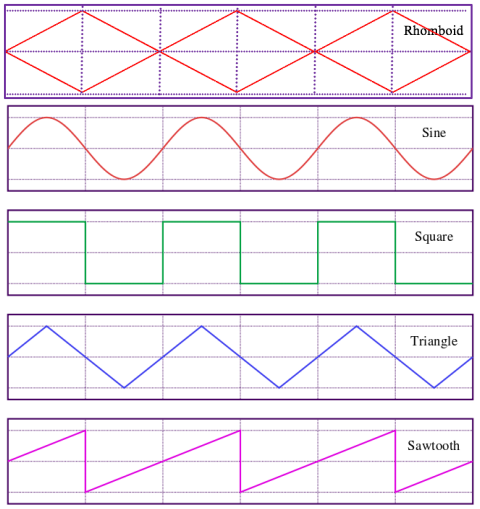
\includegraphics[width=0.7\textwidth]{waveforms}
\end{figure}

\begin{enumerate}
    \item As shown, waveforms rhomboid, square and triangle are based on a counter that counts up or down with each clock for the period of the waveform. The output of the frequency selector is the input for this module that determines the discrete incremental values of this signal (resolution).
    
    \item Generation of sine function can be somewhat different. The following second order differential equation can be used to generate the sine function:
    \begin{gather*}
    \sin(n) = \sin(n-1) + a.\cos(n-1)\\
    \cos(n) = \cos(n-1) - a.\sin(n)
    \end{gather*}
    
    In order to do the mathematical operations with reasonable accuracy, operations are done in 16-bit fixed point. Also, considering the period of about 256 clock cycles from frequency selector, the equations turn to:
    \begin{gather*}
    \sin(n) = \sin(n-1) + \frac{1}{64}.\cos(n-1)\\
    \cos(n) = \cos(n-1) - \frac{1}{64}.\sin(n)
    \end{gather*}
    Assuming values are between -32768 to 32767 for $\sin$ and $\cos$.

    Initialization of first values in differential equations is necessary. Use $0$ for $\sin(0)$ and $30000$ for $\cos(0)$.
    The results of sine and cosine operations are signed and between -127 to +128. However, for simplification and compatibility with other parts of this experiment, we add an offset of 127, making the range of our signal between 0 and 256. 

    \item To generate the arbitrary, you should use a 1-port ROM memory to store the value of the desired signal at each increment inside the memory addresses. You will receive a file named \path{arbitray.mif} that is used for ROM initialization. 

    \Fref{fig:WGblockdia} shows the block diagram of the waveform generator module.
\end{enumerate}

\begin{figure}
    \centering
    \caption{Block diagram of waveform generator\label{fig:WGblockdia}}
    \resizebox{0.9\textwidth}{!}{%LaTeX with PSTricks extensions
%%Creator: inkscape 0.91
%%Please note this file requires PSTricks extensions
\psset{xunit=.5pt,yunit=.5pt,runit=.5pt}
\begin{pspicture}(654.94486891,252.8858365)
{
\newrgbcolor{curcolor}{0 0 0}
\pscustom[linewidth=0.59963654,linecolor=curcolor]
{
\newpath
\moveto(468.61600121,71.19583599)
\lineto(468.61600121,26.52283743)
}
}
{
\newrgbcolor{curcolor}{0 0 0}
\pscustom[linewidth=0.59963654,linecolor=curcolor]
{
\newpath
\moveto(513.28898913,71.19583599)
\lineto(513.28898913,26.52283743)
}
}
{
\newrgbcolor{curcolor}{1 1 1}
\pscustom[linestyle=none,fillstyle=solid,fillcolor=curcolor]
{
\newpath
\moveto(424.24298965,26.52283743)
\lineto(424.24298965,-3.45916358)
\lineto(572.9530006,-3.45916358)
\lineto(572.9530006,26.52283743)
\lineto(424.24298965,26.52283743)
\closepath
}
}
{
\newrgbcolor{curcolor}{0 0 0}
\pscustom[linewidth=0.59963654,linecolor=curcolor]
{
\newpath
\moveto(424.24298965,26.52283743)
\lineto(572.9530006,26.52283743)
\lineto(572.9530006,-3.45916358)
\lineto(424.24298965,-3.45916358)
\closepath
}
}
{
\newrgbcolor{curcolor}{1 1 1}
\pscustom[linestyle=none,fillstyle=solid,fillcolor=curcolor]
{
\newpath
\moveto(472.15799725,18.95283826)
\lineto(472.15799725,5.01083913)
\lineto(525.05698513,5.01083913)
\lineto(525.05698513,18.95283826)
\lineto(472.15799725,18.95283826)
\closepath
}
}
{
\newrgbcolor{curcolor}{0 0 0}
\pscustom[linestyle=none,fillstyle=solid,fillcolor=curcolor]
{
\newpath
\moveto(473.37777385,10.52360177)
\lineto(474.5003019,10.6217463)
\curveto(474.55346351,10.17191721)(474.67614418,9.80183055)(474.86834388,9.51148632)
\curveto(475.06463293,9.22523145)(475.36724523,8.99213819)(475.77618077,8.81220656)
\curveto(476.1851163,8.63636427)(476.64516878,8.54844313)(477.1563382,8.54844313)
\curveto(477.61025665,8.54844313)(478.01101347,8.6159175)(478.35860868,8.75086622)
\curveto(478.70620388,8.88581495)(478.96383327,9.06983594)(479.13149684,9.3029292)
\curveto(479.30324977,9.54011181)(479.38912623,9.7977412)(479.38912623,10.07581736)
\curveto(479.38912623,10.35798288)(479.30733912,10.6033442)(479.14376491,10.81190133)
\curveto(478.98019069,11.02454781)(478.71029324,11.20243476)(478.33407255,11.3455622)
\curveto(478.09280058,11.43961737)(477.5591397,11.58478949)(476.73308992,11.78107855)
\curveto(475.90704014,11.98145696)(475.32839636,12.16956731)(474.99715857,12.34540959)
\curveto(474.56777626,12.57032413)(474.24676186,12.8484003)(474.03411538,13.17963808)
\curveto(473.82555826,13.51496522)(473.7212797,13.88914124)(473.7212797,14.30216613)
\curveto(473.7212797,14.75608457)(473.85009439,15.17933285)(474.10772378,15.57191097)
\curveto(474.36535317,15.96857844)(474.74157386,16.26914606)(475.23638586,16.47361382)
\curveto(475.73119786,16.67808159)(476.28121615,16.78031548)(476.88644075,16.78031548)
\curveto(477.55300567,16.78031548)(478.13982817,16.67194756)(478.64690823,16.45521172)
\curveto(479.15807765,16.24256525)(479.55065577,15.92768488)(479.82464257,15.51057064)
\curveto(480.09862938,15.09345639)(480.24584618,14.62113584)(480.26629295,14.093609)
\lineto(479.12536281,14.00773254)
\curveto(479.06402248,14.57615294)(478.85546535,15.00553525)(478.49969144,15.29587948)
\curveto(478.14800688,15.58622371)(477.62661407,15.73139583)(476.93551301,15.73139583)
\curveto(476.21578647,15.73139583)(475.6903043,15.59849178)(475.35906652,15.33268368)
\curveto(475.03191809,15.07096493)(474.86834388,14.75403989)(474.86834388,14.38190856)
\curveto(474.86834388,14.05884948)(474.98489051,13.79304138)(475.21798376,13.58448426)
\curveto(475.44698766,13.37592714)(476.04403354,13.16123598)(477.00912141,12.94041079)
\curveto(477.97829863,12.72367496)(478.64281888,12.53351993)(479.00268215,12.36994572)
\curveto(479.52611963,12.12867375)(479.91256371,11.8219721)(480.16201439,11.44984076)
\curveto(480.41146507,11.08179878)(480.53619041,10.65650582)(480.53619041,10.17396189)
\curveto(480.53619041,9.69550731)(480.399197,9.24363355)(480.12521019,8.81834059)
\curveto(479.85122338,8.39713699)(479.45660059,8.06794388)(478.94134182,7.83076127)
\curveto(478.4301724,7.59766801)(477.85357329,7.48112139)(477.2115445,7.48112139)
\curveto(476.39776278,7.48112139)(475.71484044,7.59971269)(475.16277746,7.8368953)
\curveto(474.61480385,8.07407791)(474.18337685,8.42985183)(473.86849649,8.90421705)
\curveto(473.55770548,9.38267163)(473.39413127,9.92246654)(473.37777385,10.52360177)
\closepath
}
}
{
\newrgbcolor{curcolor}{0 0 0}
\pscustom[linestyle=none,fillstyle=solid,fillcolor=curcolor]
{
\newpath
\moveto(483.71975357,7.63447221)
\lineto(481.33361472,16.62696465)
\lineto(482.55428729,16.62696465)
\lineto(483.92217666,10.7321589)
\curveto(484.06939345,10.11466624)(484.19616347,9.50126293)(484.30248671,8.89194898)
\curveto(484.53149061,9.85294749)(484.66643934,10.40705515)(484.70733289,10.55427194)
\lineto(486.41872811,16.62696465)
\lineto(487.85409184,16.62696465)
\lineto(489.14223878,12.07551213)
\curveto(489.46529785,10.94685005)(489.69839111,9.88566234)(489.84151855,8.89194898)
\curveto(489.9560205,9.46036938)(490.10528197,10.11262156)(490.28930296,10.84870552)
\lineto(491.70013056,16.62696465)
\lineto(492.896267,16.62696465)
\lineto(490.43038572,7.63447221)
\lineto(489.28332154,7.63447221)
\lineto(487.38790533,14.48618712)
\curveto(487.22842047,15.05869687)(487.1343653,15.41038143)(487.10573981,15.5412408)
\curveto(487.01168464,15.12821591)(486.9237635,14.77653135)(486.84197639,14.48618712)
\lineto(484.93429211,7.63447221)
\lineto(483.71975357,7.63447221)
\closepath
}
}
{
\newrgbcolor{curcolor}{0 0 0}
\pscustom[linestyle=none,fillstyle=solid,fillcolor=curcolor]
{
\newpath
\moveto(493.88384677,5.13792076)
\lineto(493.88384677,16.62696465)
\lineto(496.31905788,16.62696465)
\lineto(496.31905788,15.71299373)
\lineto(494.98797271,15.71299373)
\lineto(494.98797271,6.05189169)
\lineto(496.31905788,6.05189169)
\lineto(496.31905788,5.13792076)
\lineto(493.88384677,5.13792076)
\closepath
}
}
{
\newrgbcolor{curcolor}{0 0 0}
\pscustom[linestyle=none,fillstyle=solid,fillcolor=curcolor]
{
\newpath
\moveto(501.22014898,7.63447221)
\lineto(500.11602303,7.63447221)
\lineto(500.11602303,14.67020811)
\curveto(499.85021494,14.41666808)(499.50057505,14.16312804)(499.06710338,13.90958801)
\curveto(498.63772107,13.65604798)(498.25127699,13.46589296)(497.90777114,13.33912294)
\lineto(497.90777114,14.40644469)
\curveto(498.5252638,14.69678892)(499.06505871,15.04847348)(499.52715586,15.46149837)
\curveto(499.98925302,15.87452326)(500.31640145,16.27528009)(500.50860115,16.66376885)
\lineto(501.22014898,16.66376885)
\lineto(501.22014898,7.63447221)
\closepath
}
}
{
\newrgbcolor{curcolor}{0 0 0}
\pscustom[linestyle=none,fillstyle=solid,fillcolor=curcolor]
{
\newpath
\moveto(504.05407138,12.0693781)
\curveto(504.05407138,13.13261049)(504.16243929,13.98728576)(504.37917513,14.63340391)
\curveto(504.60000032,15.28361141)(504.92510407,15.78455744)(505.35448638,16.13624201)
\curveto(505.78795805,16.48792657)(506.33184231,16.66376885)(506.98613917,16.66376885)
\curveto(507.4686831,16.66376885)(507.89193138,16.56562432)(508.25588401,16.36933526)
\curveto(508.61983664,16.17713556)(508.92040426,15.89701472)(509.15758687,15.52897273)
\curveto(509.39476948,15.16502011)(509.58083515,14.71928037)(509.71578387,14.19175353)
\curveto(509.8507326,13.66831605)(509.91820696,12.96085757)(509.91820696,12.0693781)
\curveto(509.91820696,11.01432442)(509.80983905,10.16169382)(509.59310321,9.51148632)
\curveto(509.37636738,8.86536817)(509.05126363,8.36442214)(508.61779196,8.00864823)
\curveto(508.18840965,7.65696367)(507.64452538,7.48112139)(506.98613917,7.48112139)
\curveto(506.11919583,7.48112139)(505.43831817,7.79191239)(504.94350617,8.41349441)
\curveto(504.35054964,9.16184644)(504.05407138,10.38047434)(504.05407138,12.0693781)
\closepath
\moveto(505.18886749,12.0693781)
\curveto(505.18886749,10.59312081)(505.36062041,9.60963085)(505.70412626,9.11890821)
\curveto(506.05172147,8.63227492)(506.47905911,8.38895828)(506.98613917,8.38895828)
\curveto(507.49321923,8.38895828)(507.91851219,8.6343196)(508.26201804,9.12504224)
\curveto(508.60961325,9.61576488)(508.78341085,10.59721017)(508.78341085,12.0693781)
\curveto(508.78341085,13.54972474)(508.60961325,14.5332147)(508.26201804,15.01984799)
\curveto(507.91851219,15.50648128)(507.48912988,15.74979792)(506.9738711,15.74979792)
\curveto(506.46679104,15.74979792)(506.06194486,15.53510677)(505.75933256,15.10572446)
\curveto(505.37902251,14.55775084)(505.18886749,13.54563538)(505.18886749,12.0693781)
\closepath
}
}
{
\newrgbcolor{curcolor}{0 0 0}
\pscustom[linestyle=none,fillstyle=solid,fillcolor=curcolor]
{
\newpath
\moveto(511.66027317,12.89133853)
\lineto(511.66027317,14.1488153)
\lineto(512.91774994,14.1488153)
\lineto(512.91774994,12.89133853)
\lineto(511.66027317,12.89133853)
\closepath
\moveto(511.66027317,7.63447221)
\lineto(511.66027317,8.89194898)
\lineto(512.91774994,8.89194898)
\lineto(512.91774994,7.63447221)
\lineto(511.66027317,7.63447221)
\closepath
}
}
{
\newrgbcolor{curcolor}{0 0 0}
\pscustom[linestyle=none,fillstyle=solid,fillcolor=curcolor]
{
\newpath
\moveto(514.60460946,15.44923031)
\lineto(514.60460946,16.51041802)
\lineto(520.42580682,16.51041802)
\lineto(520.42580682,15.6516534)
\curveto(519.85329706,15.04233945)(519.28487667,14.23264709)(518.72054563,13.22257631)
\curveto(518.16030395,12.21250554)(517.72683228,11.17380928)(517.42013062,10.10648753)
\curveto(517.19930544,9.35404614)(517.05822268,8.53004104)(516.99688235,7.63447221)
\lineto(515.86208623,7.63447221)
\curveto(515.8743543,8.34193069)(516.01339238,9.19660596)(516.27920048,10.19849802)
\curveto(516.54500858,11.20039009)(516.92531863,12.16547795)(517.42013062,13.09376162)
\curveto(517.91903198,14.02613464)(518.4486035,14.81129087)(519.00884518,15.44923031)
\lineto(514.60460946,15.44923031)
\closepath
}
}
{
\newrgbcolor{curcolor}{0 0 0}
\pscustom[linestyle=none,fillstyle=solid,fillcolor=curcolor]
{
\newpath
\moveto(523.67684515,5.13792076)
\lineto(521.24163403,5.13792076)
\lineto(521.24163403,6.05189169)
\lineto(522.5727192,6.05189169)
\lineto(522.5727192,15.71299373)
\lineto(521.24163403,15.71299373)
\lineto(521.24163403,16.62696465)
\lineto(523.67684515,16.62696465)
\lineto(523.67684515,5.13792076)
\closepath
}
}
{
\newrgbcolor{curcolor}{0 0 0}
\pscustom[linewidth=0.59963654,linecolor=curcolor]
{
\newpath
\moveto(491.10200501,48.70983927)
\lineto(491.10200501,26.52283743)
}
}
{
\newrgbcolor{curcolor}{0 0 0}
\pscustom[linewidth=0.59963654,linecolor=curcolor]
{
\newpath
\moveto(513.28898913,71.19583599)
\lineto(483.60698931,71.19583599)
}
}
{
\newrgbcolor{curcolor}{0 0 0}
\pscustom[linewidth=0.59963654,linecolor=curcolor]
{
\newpath
\moveto(483.60698931,71.19583599)
\lineto(483.60698931,93.38283783)
}
}
{
\newrgbcolor{curcolor}{0 0 0}
\pscustom[linewidth=0.59963654,linecolor=curcolor]
{
\newpath
\moveto(483.60698931,93.38283783)
\lineto(498.59801284,93.38283783)
}
}
{
\newrgbcolor{curcolor}{0 0 0}
\pscustom[linewidth=0.59963654,linecolor=curcolor]
{
\newpath
\moveto(513.28898913,78.3918391)
\lineto(498.29800103,78.3918391)
\lineto(498.29800103,108.37383656)
\lineto(513.28898913,108.37383656)
\curveto(521.38399302,108.37383656)(528.28001267,101.47783817)(528.28001267,93.38283783)
\curveto(528.28001267,85.28783748)(521.38399302,78.3918391)(513.28898913,78.3918391)
}
}
{
\newrgbcolor{curcolor}{0 0 0}
\pscustom[linewidth=0.59963654,linecolor=curcolor]
{
\newpath
\moveto(468.61600121,100.87783581)
\lineto(498.59801284,100.87783581)
}
}
{
\newrgbcolor{curcolor}{0 0 0}
\pscustom[linewidth=0.59963654,linecolor=curcolor]
{
\newpath
\moveto(468.61600121,71.19583599)
\lineto(468.61600121,100.87783581)
}
}
{
\newrgbcolor{curcolor}{0 0 0}
\pscustom[linewidth=0.59963654,linecolor=curcolor]
{
\newpath
\moveto(528.28001267,93.38283783)
\lineto(550.46600467,93.38283783)
}
}
{
\newrgbcolor{curcolor}{0 0 0}
\pscustom[linewidth=0.59963654,linecolor=curcolor]
{
\newpath
\moveto(550.46600467,115.86883809)
\lineto(550.46600467,93.38283783)
}
}
{
\newrgbcolor{curcolor}{1 1 1}
\pscustom[linestyle=none,fillstyle=solid,fillcolor=curcolor]
{
\newpath
\moveto(527.98000086,108.37383656)
\lineto(527.98000086,152.74683748)
\lineto(557.9620125,138.05583639)
\lineto(557.9620125,123.06483765)
\lineto(527.98000086,108.37383656)
\closepath
}
}
{
\newrgbcolor{curcolor}{0 0 0}
\pscustom[linewidth=0.59963654,linecolor=curcolor]
{
\newpath
\moveto(527.98000086,108.37383656)
\lineto(527.98000086,152.74683748)
\lineto(557.9620125,138.05583639)
\lineto(557.9620125,123.06483765)
\lineto(527.98000086,108.37383656)
\closepath
}
}
{
\newrgbcolor{curcolor}{1 1 1}
\pscustom[linestyle=none,fillstyle=solid,fillcolor=curcolor]
{
\newpath
\moveto(312.70999778,197.7192384)
\lineto(312.70999778,138.35483835)
\lineto(446.42898165,138.35483835)
\lineto(446.42898165,197.7192384)
\lineto(312.70999778,197.7192384)
\closepath
}
}
{
\newrgbcolor{curcolor}{0 0 0}
\pscustom[linewidth=0.59963654,linecolor=curcolor]
{
\newpath
\moveto(312.70999778,197.7192384)
\lineto(446.42898165,197.7192384)
\lineto(446.42898165,138.35483835)
\lineto(312.70999778,138.35483835)
\closepath
}
}
{
\newrgbcolor{curcolor}{1 1 1}
\pscustom[linestyle=none,fillstyle=solid,fillcolor=curcolor]
{
\newpath
\moveto(350.63699678,175.45773853)
\lineto(350.63699678,161.51623546)
\lineto(408.52098187,161.51623546)
\lineto(408.52098187,175.45773853)
\lineto(350.63699678,175.45773853)
\closepath
}
}
{
\newrgbcolor{curcolor}{0 0 0}
\pscustom[linestyle=none,fillstyle=solid,fillcolor=curcolor]
{
\newpath
\moveto(352.3562021,164.13962198)
\lineto(352.3562021,173.13211442)
\lineto(355.74832237,173.13211442)
\curveto(356.34536826,173.13211442)(356.80133138,173.10348893)(357.11621174,173.04623796)
\curveto(357.55786212,172.97262956)(357.92794878,172.8315468)(358.22647172,172.62298968)
\curveto(358.52499466,172.41852191)(358.76422195,172.13022236)(358.94415359,171.75809102)
\curveto(359.12817458,171.38595968)(359.22018507,170.97702414)(359.22018507,170.53128441)
\curveto(359.22018507,169.76657496)(358.97686843,169.11841213)(358.49023514,168.58679594)
\curveto(358.00360186,168.05926909)(357.12439045,167.79550567)(355.85260094,167.79550567)
\lineto(353.54620451,167.79550567)
\lineto(353.54620451,164.13962198)
\lineto(352.3562021,164.13962198)
\closepath
\moveto(353.54620451,168.85669339)
\lineto(355.87100303,168.85669339)
\curveto(356.63980184,168.85669339)(357.18573078,168.99982083)(357.50878986,169.2860757)
\curveto(357.83184893,169.57233058)(357.99337847,169.97513208)(357.99337847,170.49448021)
\curveto(357.99337847,170.87070091)(357.89727862,171.1917153)(357.70507891,171.4575234)
\curveto(357.51696857,171.72742085)(357.26751789,171.90530781)(356.95672688,171.99118427)
\curveto(356.75634847,172.04434589)(356.38626181,172.0709267)(355.8464669,172.0709267)
\lineto(353.54620451,172.0709267)
\lineto(353.54620451,168.85669339)
\closepath
}
}
{
\newrgbcolor{curcolor}{0 0 0}
\pscustom[linestyle=none,fillstyle=solid,fillcolor=curcolor]
{
\newpath
\moveto(360.56967236,164.13962198)
\lineto(360.56967236,170.65396507)
\lineto(361.56338571,170.65396507)
\lineto(361.56338571,169.66638575)
\curveto(361.81692574,170.12848291)(362.050019,170.43313988)(362.26266548,170.58035667)
\curveto(362.47940131,170.72757347)(362.71658392,170.80118186)(362.97421331,170.80118186)
\curveto(363.34634465,170.80118186)(363.72461002,170.68259056)(364.10900942,170.44540795)
\lineto(363.72869937,169.42102443)
\curveto(363.45880192,169.58050929)(363.18890447,169.66025172)(362.91900701,169.66025172)
\curveto(362.67773505,169.66025172)(362.46099921,169.58664332)(362.26879951,169.43942653)
\curveto(362.07659981,169.29629909)(361.9396064,169.09592068)(361.8578193,168.83829129)
\curveto(361.73513864,168.44571318)(361.67379831,168.01633086)(361.67379831,167.55014435)
\lineto(361.67379831,164.13962198)
\lineto(360.56967236,164.13962198)
\closepath
}
}
{
\newrgbcolor{curcolor}{0 0 0}
\pscustom[linestyle=none,fillstyle=solid,fillcolor=curcolor]
{
\newpath
\moveto(364.34210271,167.39679353)
\curveto(364.34210271,168.60315336)(364.67742985,169.4966775)(365.34808413,170.07736597)
\curveto(365.90832581,170.5599099)(366.59124816,170.80118186)(367.39685116,170.80118186)
\curveto(368.29241999,170.80118186)(369.0244146,170.50674828)(369.59283499,169.91788111)
\curveto(370.16125539,169.33310329)(370.44546558,168.52341093)(370.44546558,167.48880402)
\curveto(370.44546558,166.65048617)(370.31869557,165.99005528)(370.06515554,165.50751135)
\curveto(369.81570486,165.02905677)(369.44970755,164.65692543)(368.96716362,164.39111734)
\curveto(368.48870904,164.12530924)(367.96527156,163.99240519)(367.39685116,163.99240519)
\curveto(366.48492492,163.99240519)(365.74679627,164.2847941)(365.18246524,164.86957191)
\curveto(364.62222355,165.45434973)(364.34210271,166.29675693)(364.34210271,167.39679353)
\closepath
\moveto(365.47689882,167.39679353)
\curveto(365.47689882,166.56256503)(365.65887513,165.93689366)(366.02282776,165.51977942)
\curveto(366.38678039,165.10675452)(366.84478819,164.90024208)(367.39685116,164.90024208)
\curveto(367.94482478,164.90024208)(368.4007879,165.1087992)(368.76474053,165.52591345)
\curveto(369.12869316,165.9430277)(369.31066947,166.57892245)(369.31066947,167.43359772)
\curveto(369.31066947,168.23920073)(369.12664848,168.84851468)(368.7586065,169.26153957)
\curveto(368.39465387,169.67865382)(367.94073543,169.88721094)(367.39685116,169.88721094)
\curveto(366.84478819,169.88721094)(366.38678039,169.6806985)(366.02282776,169.2676736)
\curveto(365.65887513,168.85464871)(365.47689882,168.23102202)(365.47689882,167.39679353)
\closepath
}
}
{
\newrgbcolor{curcolor}{0 0 0}
\pscustom[linestyle=none,fillstyle=solid,fillcolor=curcolor]
{
\newpath
\moveto(375.99676546,166.52576083)
\lineto(377.08248931,166.38467807)
\curveto(376.963898,165.63632604)(376.65924103,165.04950355)(376.16851839,164.62421059)
\curveto(375.6818851,164.20300699)(375.08279454,163.99240519)(374.37124671,163.99240519)
\curveto(373.47976724,163.99240519)(372.76208537,164.28274942)(372.21820111,164.86343788)
\curveto(371.6784062,165.4482157)(371.40850875,166.28448887)(371.40850875,167.37225739)
\curveto(371.40850875,168.07562652)(371.52505537,168.6910745)(371.75814863,169.21860134)
\curveto(371.99124189,169.74612818)(372.34497112,170.14075097)(372.81933635,170.40246972)
\curveto(373.29779092,170.66827781)(373.81713905,170.80118186)(374.37738074,170.80118186)
\curveto(375.08483922,170.80118186)(375.663483,170.62125023)(376.11331209,170.26138696)
\curveto(376.56314118,169.90561304)(376.85144073,169.39853298)(376.97821075,168.74014676)
\lineto(375.90475497,168.57452787)
\curveto(375.80252108,169.01208889)(375.62054477,169.341282)(375.35882603,169.56210719)
\curveto(375.10119664,169.78293238)(374.78836095,169.89334497)(374.42031897,169.89334497)
\curveto(373.86416664,169.89334497)(373.41229287,169.69296656)(373.06469767,169.29220974)
\curveto(372.71710246,168.89554227)(372.54330486,168.26578154)(372.54330486,167.40292756)
\curveto(372.54330486,166.52780551)(372.71096843,165.89191075)(373.04629557,165.49524328)
\curveto(373.38162271,165.09857581)(373.81918373,164.90024208)(374.35897864,164.90024208)
\curveto(374.79245031,164.90024208)(375.15435826,165.03314613)(375.44470249,165.29895423)
\curveto(375.73504672,165.56476232)(375.91906771,165.97369786)(375.99676546,166.52576083)
\closepath
}
}
{
\newrgbcolor{curcolor}{0 0 0}
\pscustom[linestyle=none,fillstyle=solid,fillcolor=curcolor]
{
\newpath
\moveto(382.48657284,166.23746128)
\lineto(383.62750299,166.09637852)
\curveto(383.44757135,165.4298136)(383.11428889,164.91251014)(382.6276556,164.54446816)
\curveto(382.14102231,164.17642618)(381.5194403,163.99240519)(380.76290956,163.99240519)
\curveto(379.81008976,163.99240519)(379.05355902,164.2847941)(378.49331733,164.86957191)
\curveto(377.937165,165.45843909)(377.65908884,166.28244419)(377.65908884,167.34158723)
\curveto(377.65908884,168.43753447)(377.94125436,169.28812038)(378.5055854,169.89334497)
\curveto(379.06991644,170.49856957)(379.80191105,170.80118186)(380.70156923,170.80118186)
\curveto(381.57260192,170.80118186)(382.28414975,170.5047036)(382.83621272,169.91174707)
\curveto(383.3882757,169.31879055)(383.66430718,168.48456205)(383.66430718,167.40906159)
\curveto(383.66430718,167.34363191)(383.66226251,167.24548738)(383.65817315,167.11462801)
\lineto(378.80001898,167.11462801)
\curveto(378.84091254,166.39899082)(379.04333563,165.8510172)(379.40728825,165.47070715)
\curveto(379.77124088,165.0903971)(380.22515933,164.90024208)(380.76904359,164.90024208)
\curveto(381.17388977,164.90024208)(381.5194403,165.00656532)(381.80569517,165.2192118)
\curveto(382.09195005,165.43185828)(382.31890927,165.77127477)(382.48657284,166.23746128)
\closepath
\moveto(378.86135931,168.0224649)
\lineto(382.49884091,168.0224649)
\curveto(382.44976864,168.57043851)(382.31073056,168.98141873)(382.08172666,169.25540554)
\curveto(381.7300421,169.6806985)(381.27407898,169.89334497)(380.71383729,169.89334497)
\curveto(380.20675723,169.89334497)(379.77941959,169.72363673)(379.43182439,169.38422023)
\curveto(379.08831854,169.04480374)(378.89816351,168.59088529)(378.86135931,168.0224649)
\closepath
}
}
{
\newrgbcolor{curcolor}{0 0 0}
\pscustom[linestyle=none,fillstyle=solid,fillcolor=curcolor]
{
\newpath
\moveto(384.57827893,166.08411046)
\lineto(385.67013681,166.25586338)
\curveto(385.73147714,165.81830236)(385.90118539,165.48297522)(386.17926155,165.24988196)
\curveto(386.46142707,165.01678871)(386.85400519,164.90024208)(387.3569959,164.90024208)
\curveto(387.86407596,164.90024208)(388.24029665,165.00247596)(388.48565798,165.20694373)
\curveto(388.7310193,165.41550085)(388.85369996,165.6588175)(388.85369996,165.93689366)
\curveto(388.85369996,166.18634434)(388.74533204,166.3826334)(388.52859621,166.52576083)
\curveto(388.37729006,166.62390536)(388.00106936,166.7486307)(387.39993413,166.89993685)
\curveto(386.59024177,167.10440462)(386.0279554,167.2802469)(385.71307504,167.42746369)
\curveto(385.40228403,167.57876984)(385.16510142,167.78528229)(385.00152721,168.04700103)
\curveto(384.84204235,168.31280913)(384.76229992,168.60519804)(384.76229992,168.92416775)
\curveto(384.76229992,169.21451198)(384.82772961,169.48236476)(384.95858898,169.72772608)
\curveto(385.0935377,169.97717676)(385.27551402,170.1836892)(385.50451792,170.34726342)
\curveto(385.67627084,170.47403344)(385.9093641,170.58035667)(386.20379768,170.66623314)
\curveto(386.50232063,170.75619895)(386.82129034,170.80118186)(387.16070684,170.80118186)
\curveto(387.67187626,170.80118186)(388.11966067,170.72757347)(388.50406007,170.58035667)
\curveto(388.89254883,170.43313988)(389.17880371,170.23276147)(389.3628247,169.97922144)
\curveto(389.54684569,169.72977076)(389.67361571,169.39444362)(389.74313475,168.97324002)
\lineto(388.66354493,168.82602322)
\curveto(388.61447267,169.16135036)(388.47134523,169.42306911)(388.23416262,169.61117945)
\curveto(388.00106936,169.7992898)(387.66983158,169.89334497)(387.24044927,169.89334497)
\curveto(386.7333692,169.89334497)(386.37146125,169.80951319)(386.15472542,169.64184962)
\curveto(385.93798959,169.47418605)(385.82962167,169.27789699)(385.82962167,169.05298245)
\curveto(385.82962167,168.90985501)(385.87460458,168.78104032)(385.9645704,168.66653837)
\curveto(386.05453621,168.54794706)(386.19561897,168.44980253)(386.38781868,168.37210478)
\curveto(386.49823127,168.33121123)(386.82333502,168.23715605)(387.36312993,168.08993926)
\curveto(388.1441968,167.88138214)(388.68808107,167.70962921)(388.99478272,167.57468048)
\curveto(389.30557372,167.44382111)(389.54889037,167.25162141)(389.72473265,166.99808138)
\curveto(389.90057493,166.74454135)(389.98849607,166.42966098)(389.98849607,166.05344029)
\curveto(389.98849607,165.68539831)(389.88012815,165.3378031)(389.66339232,165.01065467)
\curveto(389.45074584,164.6875956)(389.14199951,164.43610025)(388.73715333,164.25616861)
\curveto(388.33230715,164.08032633)(387.87429935,163.99240519)(387.36312993,163.99240519)
\curveto(386.51663337,163.99240519)(385.87051522,164.16824747)(385.42477549,164.51993203)
\curveto(384.98312511,164.87161659)(384.70095959,165.3930094)(384.57827893,166.08411046)
\closepath
}
}
{
\newrgbcolor{curcolor}{0 0 0}
\pscustom[linestyle=none,fillstyle=solid,fillcolor=curcolor]
{
\newpath
\moveto(390.85952749,166.08411046)
\lineto(391.95138538,166.25586338)
\curveto(392.01272571,165.81830236)(392.18243395,165.48297522)(392.46051012,165.24988196)
\curveto(392.74267564,165.01678871)(393.13525375,164.90024208)(393.63824446,164.90024208)
\curveto(394.14532453,164.90024208)(394.52154522,165.00247596)(394.76690654,165.20694373)
\curveto(395.01226786,165.41550085)(395.13494852,165.6588175)(395.13494852,165.93689366)
\curveto(395.13494852,166.18634434)(395.02658061,166.3826334)(394.80984477,166.52576083)
\curveto(394.65853862,166.62390536)(394.28231793,166.7486307)(393.68118269,166.89993685)
\curveto(392.87149033,167.10440462)(392.30920397,167.2802469)(391.99432361,167.42746369)
\curveto(391.6835326,167.57876984)(391.44634999,167.78528229)(391.28277577,168.04700103)
\curveto(391.12329092,168.31280913)(391.04354849,168.60519804)(391.04354849,168.92416775)
\curveto(391.04354849,169.21451198)(391.10897817,169.48236476)(391.23983754,169.72772608)
\curveto(391.37478627,169.97717676)(391.55676258,170.1836892)(391.78576648,170.34726342)
\curveto(391.95751941,170.47403344)(392.19061266,170.58035667)(392.48504625,170.66623314)
\curveto(392.78356919,170.75619895)(393.10253891,170.80118186)(393.4419554,170.80118186)
\curveto(393.95312482,170.80118186)(394.40090924,170.72757347)(394.78530864,170.58035667)
\curveto(395.1737974,170.43313988)(395.46005228,170.23276147)(395.64407327,169.97922144)
\curveto(395.82809426,169.72977076)(395.95486427,169.39444362)(396.02438332,168.97324002)
\lineto(394.9447935,168.82602322)
\curveto(394.89572124,169.16135036)(394.7525938,169.42306911)(394.51541119,169.61117945)
\curveto(394.28231793,169.7992898)(393.95108015,169.89334497)(393.52169783,169.89334497)
\curveto(393.01461777,169.89334497)(392.65270982,169.80951319)(392.43597399,169.64184962)
\curveto(392.21923815,169.47418605)(392.11087024,169.27789699)(392.11087024,169.05298245)
\curveto(392.11087024,168.90985501)(392.15585314,168.78104032)(392.24581896,168.66653837)
\curveto(392.33578478,168.54794706)(392.47686754,168.44980253)(392.66906724,168.37210478)
\curveto(392.77947984,168.33121123)(393.10458359,168.23715605)(393.6443785,168.08993926)
\curveto(394.42544537,167.88138214)(394.96932963,167.70962921)(395.27603128,167.57468048)
\curveto(395.58682229,167.44382111)(395.83013894,167.25162141)(396.00598122,166.99808138)
\curveto(396.1818235,166.74454135)(396.26974464,166.42966098)(396.26974464,166.05344029)
\curveto(396.26974464,165.68539831)(396.16137672,165.3378031)(395.94464089,165.01065467)
\curveto(395.73199441,164.6875956)(395.42324808,164.43610025)(395.0184019,164.25616861)
\curveto(394.61355572,164.08032633)(394.15554792,163.99240519)(393.6443785,163.99240519)
\curveto(392.79788194,163.99240519)(392.15176379,164.16824747)(391.70602405,164.51993203)
\curveto(391.26437368,164.87161659)(390.98220816,165.3930094)(390.85952749,166.08411046)
\closepath
}
}
{
\newrgbcolor{curcolor}{0 0 0}
\pscustom[linestyle=none,fillstyle=solid,fillcolor=curcolor]
{
\newpath
\moveto(397.17144623,167.39679353)
\curveto(397.17144623,168.60315336)(397.50677337,169.4966775)(398.17742765,170.07736597)
\curveto(398.73766933,170.5599099)(399.42059167,170.80118186)(400.22619468,170.80118186)
\curveto(401.1217635,170.80118186)(401.85375811,170.50674828)(402.42217851,169.91788111)
\curveto(402.9905989,169.33310329)(403.2748091,168.52341093)(403.2748091,167.48880402)
\curveto(403.2748091,166.65048617)(403.14803909,165.99005528)(402.89449905,165.50751135)
\curveto(402.64504838,165.02905677)(402.27905107,164.65692543)(401.79650714,164.39111734)
\curveto(401.31805256,164.12530924)(400.79461508,163.99240519)(400.22619468,163.99240519)
\curveto(399.31426844,163.99240519)(398.57613979,164.2847941)(398.01180875,164.86957191)
\curveto(397.45156707,165.45434973)(397.17144623,166.29675693)(397.17144623,167.39679353)
\closepath
\moveto(398.30624234,167.39679353)
\curveto(398.30624234,166.56256503)(398.48821865,165.93689366)(398.85217128,165.51977942)
\curveto(399.21612391,165.10675452)(399.67413171,164.90024208)(400.22619468,164.90024208)
\curveto(400.7741683,164.90024208)(401.23013142,165.1087992)(401.59408405,165.52591345)
\curveto(401.95803668,165.9430277)(402.14001299,166.57892245)(402.14001299,167.43359772)
\curveto(402.14001299,168.23920073)(401.955992,168.84851468)(401.58795002,169.26153957)
\curveto(401.22399739,169.67865382)(400.77007894,169.88721094)(400.22619468,169.88721094)
\curveto(399.67413171,169.88721094)(399.21612391,169.6806985)(398.85217128,169.2676736)
\curveto(398.48821865,168.85464871)(398.30624234,168.23102202)(398.30624234,167.39679353)
\closepath
}
}
{
\newrgbcolor{curcolor}{0 0 0}
\pscustom[linestyle=none,fillstyle=solid,fillcolor=curcolor]
{
\newpath
\moveto(404.56295686,164.13962198)
\lineto(404.56295686,170.65396507)
\lineto(405.55667021,170.65396507)
\lineto(405.55667021,169.66638575)
\curveto(405.81021025,170.12848291)(406.0433035,170.43313988)(406.25594998,170.58035667)
\curveto(406.47268581,170.72757347)(406.70986843,170.80118186)(406.96749781,170.80118186)
\curveto(407.33962915,170.80118186)(407.71789452,170.68259056)(408.10229393,170.44540795)
\lineto(407.72198388,169.42102443)
\curveto(407.45208642,169.58050929)(407.18218897,169.66025172)(406.91229152,169.66025172)
\curveto(406.67101955,169.66025172)(406.45428372,169.58664332)(406.26208401,169.43942653)
\curveto(406.06988431,169.29629909)(405.93289091,169.09592068)(405.8511038,168.83829129)
\curveto(405.72842314,168.44571318)(405.66708281,168.01633086)(405.66708281,167.55014435)
\lineto(405.66708281,164.13962198)
\lineto(404.56295686,164.13962198)
\closepath
}
}
{
\newrgbcolor{curcolor}{0 0 0}
\pscustom[linewidth=0.59963654,linecolor=curcolor]
{
\newpath
\moveto(238.35599861,168.03723857)
\lineto(305.2149998,168.03723857)
}
}
{
\newrgbcolor{curcolor}{0 0 0}
\pscustom[linestyle=none,fillstyle=solid,fillcolor=curcolor]
{
\newpath
\moveto(312.70999778,168.03723857)
\lineto(305.51499743,171.3352354)
\lineto(305.51499743,164.43943544)
\lineto(312.70999778,168.03723857)
\closepath
}
}
{
\newrgbcolor{curcolor}{0 0 0}
\pscustom[linewidth=0.59963654,linecolor=curcolor]
{
\newpath
\moveto(312.70999778,168.03723857)
\lineto(305.51499743,171.3352354)
\lineto(305.51499743,164.43943544)
\lineto(312.70999778,168.03723857)
\closepath
}
}
{
\newrgbcolor{curcolor}{0 0 0}
\pscustom[linewidth=0.59963654,linecolor=curcolor]
{
\newpath
\moveto(119.32799812,168.03723857)
\lineto(97.14109904,168.03723857)
}
}
{
\newrgbcolor{curcolor}{1 1 1}
\pscustom[linestyle=none,fillstyle=solid,fillcolor=curcolor]
{
\newpath
\moveto(67.1593,153.04633551)
\lineto(67.1593,183.02813809)
\lineto(97.14109904,168.03723857)
\lineto(67.1593,153.04633551)
\closepath
}
}
{
\newrgbcolor{curcolor}{0 0 0}
\pscustom[linewidth=0.59963654,linecolor=curcolor]
{
\newpath
\moveto(67.1593,153.04633551)
\lineto(67.1593,183.02813809)
\lineto(97.14109904,168.03723857)
\lineto(67.1593,153.04633551)
\closepath
}
}
{
\newrgbcolor{curcolor}{0 0 0}
\pscustom[linestyle=none,fillstyle=solid,fillcolor=curcolor]
{
\newpath
\moveto(87.77437926,218.48227376)
\lineto(90.20925477,217.71024006)
\curveto(89.83596376,216.35281817)(89.21381206,215.34323565)(88.34279968,214.68149248)
\curveto(87.47744323,214.02540523)(86.37736591,213.69736161)(85.04256772,213.69736161)
\curveto(83.39103775,213.69736161)(82.03361587,214.2601261)(80.97030206,215.38565508)
\curveto(79.90698824,216.51683999)(79.37533134,218.06090738)(79.37533134,220.01785727)
\curveto(79.37533134,222.08792565)(79.90981621,223.69420821)(80.97878594,224.83670497)
\curveto(82.04775568,225.98485765)(83.45325292,226.55893399)(85.19527768,226.55893399)
\curveto(86.71672138,226.55893399)(87.95254089,226.10928799)(88.90273621,225.20999599)
\curveto(89.46832866,224.67833908)(89.892523,223.91478927)(90.17531923,222.91934655)
\lineto(87.6895404,222.32547448)
\curveto(87.54248636,222.97024987)(87.23423847,223.47928308)(86.76479674,223.8525741)
\curveto(86.30101092,224.22586512)(85.73541847,224.41251063)(85.06801938,224.41251063)
\curveto(84.14610368,224.41251063)(83.39669368,224.08163904)(82.81978938,223.41989587)
\curveto(82.248541,222.7581527)(81.96291681,221.68635501)(81.96291681,220.20450278)
\curveto(81.96291681,218.63215576)(82.24571304,217.5122827)(82.81130549,216.84488361)
\curveto(83.37689794,216.17748451)(84.11216813,215.84378497)(85.01711606,215.84378497)
\curveto(85.68451515,215.84378497)(86.25859149,216.05588214)(86.73934508,216.48007648)
\curveto(87.22009866,216.90427082)(87.56511006,217.57166991)(87.77437926,218.48227376)
\closepath
}
}
{
\newrgbcolor{curcolor}{0 0 0}
\pscustom[linestyle=none,fillstyle=solid,fillcolor=curcolor]
{
\newpath
\moveto(91.19338542,222.91934655)
\lineto(93.73006758,222.91934655)
\lineto(95.88497482,216.52249591)
\lineto(97.98897875,222.91934655)
\lineto(100.4577898,222.91934655)
\lineto(97.27633226,214.24881425)
\lineto(96.70791184,212.67929519)
\curveto(96.49864263,212.15329421)(96.29785731,211.75172357)(96.10555588,211.47458327)
\curveto(95.91891037,211.19744297)(95.70115727,210.97403395)(95.45229659,210.80435621)
\curveto(95.20909184,210.62902255)(94.90649988,210.49328036)(94.54452071,210.39712965)
\curveto(94.18819746,210.30097893)(93.78379886,210.25290357)(93.3313249,210.25290357)
\curveto(92.87319501,210.25290357)(92.42354901,210.30097893)(91.9823869,210.39712965)
\lineto(91.77028973,212.26358474)
\curveto(92.14358075,212.19005772)(92.48010825,212.15329421)(92.77987225,212.15329421)
\curveto(93.33415286,212.15329421)(93.74420739,212.31731602)(94.01003584,212.64535965)
\curveto(94.27586429,212.96774734)(94.47947758,213.38062983)(94.62087569,213.88400712)
\lineto(91.19338542,222.91934655)
\closepath
}
}
{
\newrgbcolor{curcolor}{0 0 0}
\pscustom[linestyle=none,fillstyle=solid,fillcolor=curcolor]
{
\newpath
\moveto(109.8494524,220.2554061)
\lineto(107.49941576,219.83121176)
\curveto(107.42023281,220.3006535)(107.23924323,220.65414878)(106.956447,220.89169761)
\curveto(106.6793067,221.12924644)(106.31732753,221.24802085)(105.87050949,221.24802085)
\curveto(105.27663742,221.24802085)(104.80153976,221.04157961)(104.44521651,220.62869712)
\curveto(104.09454919,220.22147055)(103.91921553,219.53710368)(103.91921553,218.57559651)
\curveto(103.91921553,217.50662678)(104.09737715,216.75156085)(104.4537004,216.31039874)
\curveto(104.81567957,215.86923663)(105.29926111,215.64865557)(105.90444504,215.64865557)
\curveto(106.356919,215.64865557)(106.72738206,215.77591387)(107.01583421,216.03043048)
\curveto(107.30428636,216.290603)(107.50789964,216.73459308)(107.62667406,217.3624007)
\lineto(109.96822681,216.96365802)
\curveto(109.72502206,215.88903236)(109.25840829,215.07740719)(108.56838549,214.52878251)
\curveto(107.8783627,213.98015783)(106.95361904,213.70584549)(105.79415451,213.70584549)
\curveto(104.4763241,213.70584549)(103.42432213,214.12155595)(102.63814862,214.95297685)
\curveto(101.85763104,215.78439776)(101.46737225,216.9353784)(101.46737225,218.40591878)
\curveto(101.46737225,219.89342693)(101.860459,221.0500635)(102.64663251,221.87582848)
\curveto(103.43280602,222.70724938)(104.49611983,223.12295984)(105.83657394,223.12295984)
\curveto(106.9338233,223.12295984)(107.80483568,222.88541101)(108.44961108,222.41031335)
\curveto(109.1000424,221.94087161)(109.56665617,221.22256919)(109.8494524,220.2554061)
\closepath
}
}
{
\newrgbcolor{curcolor}{0 0 0}
\pscustom[linestyle=none,fillstyle=solid,fillcolor=curcolor]
{
\newpath
\moveto(111.63106971,213.90945878)
\lineto(111.63106971,226.34683682)
\lineto(114.0150419,226.34683682)
\lineto(114.0150419,213.90945878)
\lineto(111.63106971,213.90945878)
\closepath
}
}
{
\newrgbcolor{curcolor}{0 0 0}
\pscustom[linestyle=none,fillstyle=solid,fillcolor=curcolor]
{
\newpath
\moveto(115.89846277,218.54166097)
\curveto(115.89846277,219.3334904)(116.09359217,220.09986818)(116.48385096,220.84079429)
\curveto(116.87410975,221.5817204)(117.42556239,222.14731285)(118.13820889,222.53757165)
\curveto(118.8565113,222.92783044)(119.65682462,223.12295984)(120.53914885,223.12295984)
\curveto(121.90222666,223.12295984)(123.01927175,222.67896976)(123.89028413,221.79098961)
\curveto(124.76129651,220.90866538)(125.1968027,219.79162029)(125.1968027,218.43985433)
\curveto(125.1968027,217.07677651)(124.75564058,215.94559161)(123.87331636,215.04629961)
\curveto(122.99664806,214.15266353)(121.89091481,213.70584549)(120.55611662,213.70584549)
\curveto(119.73035164,213.70584549)(118.94135017,213.892491)(118.18911221,214.26578202)
\curveto(117.44253017,214.63907304)(116.87410975,215.18486976)(116.48385096,215.90317217)
\curveto(116.09359217,216.62713051)(115.89846277,217.50662678)(115.89846277,218.54166097)
\closepath
\moveto(118.34182217,218.41440267)
\curveto(118.34182217,217.52076659)(118.55391934,216.83639972)(118.97811368,216.36130206)
\curveto(119.40230802,215.8862044)(119.92548104,215.64865557)(120.54763273,215.64865557)
\curveto(121.16978443,215.64865557)(121.69012949,215.8862044)(122.1086679,216.36130206)
\curveto(122.53286224,216.83639972)(122.74495941,217.52642251)(122.74495941,218.43137044)
\curveto(122.74495941,219.31369467)(122.53286224,219.99240561)(122.1086679,220.46750327)
\curveto(121.69012949,220.94260093)(121.16978443,221.18014976)(120.54763273,221.18014976)
\curveto(119.92548104,221.18014976)(119.40230802,220.94260093)(118.97811368,220.46750327)
\curveto(118.55391934,219.99240561)(118.34182217,219.30803874)(118.34182217,218.41440267)
\closepath
}
}
{
\newrgbcolor{curcolor}{0 0 0}
\pscustom[linestyle=none,fillstyle=solid,fillcolor=curcolor]
{
\newpath
\moveto(135.23324125,213.90945878)
\lineto(132.84926906,213.90945878)
\lineto(132.84926906,218.50772542)
\curveto(132.84926906,219.48054444)(132.79836574,220.10835206)(132.6965591,220.39114829)
\curveto(132.59475246,220.67960044)(132.42790268,220.90300946)(132.19600978,221.06137535)
\curveto(131.9697728,221.21974123)(131.69546046,221.29892418)(131.37307276,221.29892418)
\curveto(130.96019027,221.29892418)(130.58972721,221.18580568)(130.26168359,220.9595687)
\curveto(129.93363997,220.73333172)(129.70740299,220.43356772)(129.58297265,220.0602767)
\curveto(129.46419823,219.68698568)(129.40481102,218.99696289)(129.40481102,217.99020833)
\lineto(129.40481102,213.90945878)
\lineto(127.02083883,213.90945878)
\lineto(127.02083883,222.91934655)
\lineto(129.23513329,222.91934655)
\lineto(129.23513329,221.59586021)
\curveto(130.0213068,222.61392663)(131.01109359,223.12295984)(132.20449366,223.12295984)
\curveto(132.73049465,223.12295984)(133.21124823,223.02680912)(133.64675442,222.83450769)
\curveto(134.08226061,222.64786218)(134.41030423,222.40748538)(134.63088529,222.11337731)
\curveto(134.85712227,221.81926923)(135.01266019,221.48556969)(135.09749906,221.11227867)
\curveto(135.18799385,220.73898765)(135.23324125,220.20450278)(135.23324125,219.50882406)
\lineto(135.23324125,213.90945878)
\closepath
}
}
{
\newrgbcolor{curcolor}{0 0 0}
\pscustom[linestyle=none,fillstyle=solid,fillcolor=curcolor]
{
\newpath
\moveto(142.87722509,216.77701251)
\lineto(145.2527134,216.37826984)
\curveto(144.94729347,215.50725746)(144.46371192,214.84268633)(143.80196875,214.38455644)
\curveto(143.14588151,213.93208248)(142.32294449,213.70584549)(141.3331577,213.70584549)
\curveto(139.7664666,213.70584549)(138.60700207,214.21770666)(137.85476411,215.241429)
\curveto(137.26089204,216.06153806)(136.963956,217.09657225)(136.963956,218.34653157)
\curveto(136.963956,219.83969565)(137.35421479,221.00764406)(138.13473238,221.85037682)
\curveto(138.91524996,222.6987655)(139.90220879,223.12295984)(141.09560887,223.12295984)
\curveto(142.43606298,223.12295984)(143.49372087,222.67896976)(144.26858253,221.79098961)
\curveto(145.04344419,220.90866538)(145.41390724,219.55407146)(145.3799717,217.72720784)
\lineto(139.40731539,217.72720784)
\curveto(139.42428317,217.02021727)(139.6165846,216.46876463)(139.9842197,216.07284991)
\curveto(140.35185479,215.68259112)(140.80998468,215.48746172)(141.35860936,215.48746172)
\curveto(141.73190038,215.48746172)(142.04580419,215.58926836)(142.30032079,215.79288165)
\curveto(142.55483739,215.99649493)(142.74713883,216.32453855)(142.87722509,216.77701251)
\closepath
\moveto(143.01296728,219.18643636)
\curveto(142.99599951,219.87645916)(142.81783789,220.39963218)(142.47848241,220.75595542)
\curveto(142.13912694,221.11793459)(141.72624445,221.29892418)(141.23983494,221.29892418)
\curveto(140.71948989,221.29892418)(140.28963962,221.1094507)(139.95028415,220.73050376)
\curveto(139.61092868,220.35155682)(139.4440789,219.83686768)(139.44973483,219.18643636)
\lineto(143.01296728,219.18643636)
\closepath
}
}
{
\newrgbcolor{curcolor}{0 0 0}
\pscustom[linestyle=none,fillstyle=solid,fillcolor=curcolor]
{
\newpath
\moveto(152.09072492,213.90945878)
\lineto(152.09072492,226.34683682)
\lineto(154.60195541,226.34683682)
\lineto(154.60195541,213.90945878)
\lineto(152.09072492,213.90945878)
\closepath
}
}
{
\newrgbcolor{curcolor}{0 0 0}
\pscustom[linestyle=none,fillstyle=solid,fillcolor=curcolor]
{
\newpath
\moveto(156.90957062,213.90945878)
\lineto(156.90957062,226.34683682)
\lineto(159.42080111,226.34683682)
\lineto(159.42080111,213.90945878)
\lineto(156.90957062,213.90945878)
\closepath
}
}
{
\newrgbcolor{curcolor}{0 0 0}
\pscustom[linewidth=0.59963654,linecolor=curcolor]
{
\newpath
\moveto(468.61600121,175.23293696)
\lineto(498.59801284,175.23293696)
}
}
{
\newrgbcolor{curcolor}{0 0 0}
\pscustom[linewidth=0.59963654,linecolor=curcolor]
{
\newpath
\moveto(498.59801284,175.23293696)
\lineto(498.59801284,145.55083792)
}
}
{
\newrgbcolor{curcolor}{0 0 0}
\pscustom[linewidth=0.59963654,linecolor=curcolor]
{
\newpath
\moveto(498.59801284,145.55083792)
\lineto(517.18698124,145.55083792)
}
}
{
\newrgbcolor{curcolor}{0 0 0}
\pscustom[linestyle=none,fillstyle=solid,fillcolor=curcolor]
{
\newpath
\moveto(517.18698124,150.9478367)
\lineto(528.28001267,145.55083792)
\lineto(517.18698124,140.15383559)
\closepath
}
}
{
\newrgbcolor{curcolor}{0 0 0}
\pscustom[linewidth=0.59963654,linecolor=curcolor]
{
\newpath
\moveto(517.18698124,150.9478367)
\lineto(528.28001267,145.55083792)
\lineto(517.18698124,140.15383559)
\closepath
}
}
{
\newrgbcolor{curcolor}{1 1 1}
\pscustom[linestyle=none,fillstyle=solid,fillcolor=curcolor]
{
\newpath
\moveto(223.36499988,108.37383656)
\curveto(223.36499988,112.27083654)(226.96199868,115.56883691)(230.85999787,115.56883691)
\lineto(320.20599853,115.56883691)
\curveto(324.10399772,115.56883691)(327.70099652,112.27083654)(327.70099652,108.37383656)
\lineto(327.70099652,63.40083682)
\curveto(327.70099652,59.50283763)(324.10399772,56.20483726)(320.20599853,56.20483726)
\lineto(230.85999787,56.20483726)
\curveto(226.96199868,56.20483726)(223.36499988,59.50283763)(223.36499988,63.40083682)
\lineto(223.36499988,108.37383656)
\closepath
}
}
{
\newrgbcolor{curcolor}{0 0 0}
\pscustom[linewidth=0.59963654,linecolor=curcolor]
{
\newpath
\moveto(223.36499988,108.37383656)
\curveto(223.36499988,112.27083654)(226.96199868,115.56883691)(230.85999787,115.56883691)
\lineto(320.20599853,115.56883691)
\curveto(324.10399772,115.56883691)(327.70099652,112.27083654)(327.70099652,108.37383656)
\lineto(327.70099652,63.40083682)
\curveto(327.70099652,59.50283763)(324.10399772,56.20483726)(320.20599853,56.20483726)
\lineto(230.85999787,56.20483726)
\curveto(226.96199868,56.20483726)(223.36499988,59.50283763)(223.36499988,63.40083682)
\lineto(223.36499988,108.37383656)
}
}
{
\newrgbcolor{curcolor}{1 1 1}
\pscustom[linestyle=none,fillstyle=solid,fillcolor=curcolor]
{
\newpath
\moveto(258.74299692,100.74683621)
\lineto(258.74299692,86.78683708)
\lineto(292.34199869,86.78683708)
\lineto(292.34199869,100.74683621)
\lineto(258.74299692,100.74683621)
\closepath
}
}
{
\newrgbcolor{curcolor}{0 0 0}
\pscustom[linestyle=none,fillstyle=solid,fillcolor=curcolor]
{
\newpath
\moveto(264.02308407,89.48487355)
\lineto(262.91895812,89.48487355)
\lineto(262.91895812,96.52060944)
\curveto(262.65315003,96.26706941)(262.30351014,96.01352938)(261.87003847,95.75998935)
\curveto(261.44065616,95.50644931)(261.05421208,95.31629429)(260.71070623,95.18952427)
\lineto(260.71070623,96.25684602)
\curveto(261.32819889,96.54719025)(261.8679938,96.89887481)(262.33009095,97.31189971)
\curveto(262.79218811,97.7249246)(263.11933654,98.12568142)(263.31153624,98.51417018)
\lineto(264.02308407,98.51417018)
\lineto(264.02308407,89.48487355)
\closepath
}
}
{
\newrgbcolor{curcolor}{0 0 0}
\pscustom[linestyle=none,fillstyle=solid,fillcolor=curcolor]
{
\newpath
\moveto(266.73432665,92.18384808)
\lineto(266.73432665,93.29410806)
\lineto(270.12644692,93.29410806)
\lineto(270.12644692,92.18384808)
\lineto(266.73432665,92.18384808)
\closepath
}
}
{
\newrgbcolor{curcolor}{0 0 0}
\pscustom[linestyle=none,fillstyle=solid,fillcolor=curcolor]
{
\newpath
\moveto(271.33485146,86.9883221)
\lineto(271.33485146,95.99921663)
\lineto(272.34083288,95.99921663)
\lineto(272.34083288,95.15272007)
\curveto(272.57801549,95.48395786)(272.84586827,95.73136386)(273.14439121,95.89493807)
\curveto(273.44291415,96.06260164)(273.8048221,96.14643343)(274.23011506,96.14643343)
\curveto(274.78626739,96.14643343)(275.27699003,96.00330599)(275.70228299,95.71705111)
\curveto(276.12757594,95.43079624)(276.44859034,95.02595006)(276.66532617,94.50251257)
\curveto(276.88206201,93.98316444)(276.99042992,93.41269937)(276.99042992,92.79111735)
\curveto(276.99042992,92.12455243)(276.86979394,91.52341719)(276.62852198,90.98771164)
\curveto(276.39133936,90.45609544)(276.04374416,90.04715991)(275.58573636,89.76090503)
\curveto(275.13181791,89.47873951)(274.65336334,89.33765675)(274.15037263,89.33765675)
\curveto(273.78233064,89.33765675)(273.45109286,89.4153545)(273.15665927,89.57075001)
\curveto(272.86631504,89.72614551)(272.62708776,89.92243457)(272.43897741,90.15961718)
\lineto(272.43897741,86.9883221)
\lineto(271.33485146,86.9883221)
\closepath
\moveto(272.33469885,92.70524089)
\curveto(272.33469885,91.86692304)(272.50440709,91.24738571)(272.84382359,90.84662888)
\curveto(273.18324008,90.44587205)(273.5942203,90.24549364)(274.07676423,90.24549364)
\curveto(274.56748687,90.24549364)(274.9866458,90.45200609)(275.334241,90.86503098)
\curveto(275.68592556,91.28214523)(275.86176785,91.9262187)(275.86176785,92.79725139)
\curveto(275.86176785,93.62739053)(275.69001492,94.24897254)(275.34650907,94.66199743)
\curveto(275.00709258,95.07502232)(274.60020172,95.28153477)(274.12583649,95.28153477)
\curveto(273.65556063,95.28153477)(273.23844638,95.06070958)(272.87449375,94.6190592)
\curveto(272.51463048,94.18149818)(272.33469885,93.54355874)(272.33469885,92.70524089)
\closepath
}
}
{
\newrgbcolor{curcolor}{0 0 0}
\pscustom[linestyle=none,fillstyle=solid,fillcolor=curcolor]
{
\newpath
\moveto(277.94120582,92.74204509)
\curveto(277.94120582,93.94840492)(278.27653296,94.84192907)(278.94718724,95.42261753)
\curveto(279.50742892,95.90516146)(280.19035127,96.14643343)(280.99595428,96.14643343)
\curveto(281.8915231,96.14643343)(282.62351771,95.85199984)(283.1919381,95.26313267)
\curveto(283.7603585,94.67835485)(284.0445687,93.86866249)(284.0445687,92.83405559)
\curveto(284.0445687,91.99573774)(283.91779868,91.33530685)(283.66425865,90.85276291)
\curveto(283.41480797,90.37430834)(283.04881067,90.002177)(282.56626673,89.7363689)
\curveto(282.08781216,89.4705608)(281.56437467,89.33765675)(280.99595428,89.33765675)
\curveto(280.08402803,89.33765675)(279.34589939,89.63004566)(278.78156835,90.21482348)
\curveto(278.22132666,90.79960129)(277.94120582,91.6420085)(277.94120582,92.74204509)
\closepath
\moveto(279.07600193,92.74204509)
\curveto(279.07600193,91.9078166)(279.25797825,91.28214523)(279.62193087,90.86503098)
\curveto(279.9858835,90.45200609)(280.4438913,90.24549364)(280.99595428,90.24549364)
\curveto(281.54392789,90.24549364)(281.99989102,90.45405077)(282.36384364,90.87116501)
\curveto(282.72779627,91.28827926)(282.90977258,91.92417402)(282.90977258,92.77884929)
\curveto(282.90977258,93.58445229)(282.72575159,94.19376624)(282.35770961,94.60679113)
\curveto(281.99375698,95.02390538)(281.53983854,95.2324625)(280.99595428,95.2324625)
\curveto(280.4438913,95.2324625)(279.9858835,95.02595006)(279.62193087,94.61292517)
\curveto(279.25797825,94.19990028)(279.07600193,93.57627358)(279.07600193,92.74204509)
\closepath
}
}
{
\newrgbcolor{curcolor}{0 0 0}
\pscustom[linestyle=none,fillstyle=solid,fillcolor=curcolor]
{
\newpath
\moveto(285.33271477,89.48487355)
\lineto(285.33271477,95.99921663)
\lineto(286.32642812,95.99921663)
\lineto(286.32642812,95.01163731)
\curveto(286.57996815,95.47373447)(286.81306141,95.77839144)(287.02570789,95.92560824)
\curveto(287.24244372,96.07282503)(287.47962633,96.14643343)(287.73725572,96.14643343)
\curveto(288.10938706,96.14643343)(288.48765243,96.02784212)(288.87205183,95.79065951)
\lineto(288.49174178,94.76627599)
\curveto(288.22184433,94.92576085)(287.95194687,95.00550328)(287.68204942,95.00550328)
\curveto(287.44077745,95.00550328)(287.22404162,94.93189489)(287.03184192,94.78467809)
\curveto(286.83964222,94.64155065)(286.70264881,94.44117224)(286.62086171,94.18354285)
\curveto(286.49818104,93.79096474)(286.43684071,93.36158243)(286.43684071,92.89539592)
\lineto(286.43684071,89.48487355)
\lineto(285.33271477,89.48487355)
\closepath
}
}
{
\newrgbcolor{curcolor}{0 0 0}
\pscustom[linestyle=none,fillstyle=solid,fillcolor=curcolor]
{
\newpath
\moveto(291.92680116,90.47245286)
\lineto(292.08628602,89.49714161)
\curveto(291.77549501,89.43171193)(291.49741885,89.39899708)(291.25205753,89.39899708)
\curveto(290.8513007,89.39899708)(290.54050969,89.46238209)(290.3196845,89.58915211)
\curveto(290.09885931,89.71592212)(289.94346381,89.88154101)(289.85349799,90.08600878)
\curveto(289.76353217,90.29456591)(289.71854927,90.73008225)(289.71854927,91.39255782)
\lineto(289.71854927,95.14045201)
\lineto(288.9088569,95.14045201)
\lineto(288.9088569,95.99921663)
\lineto(289.71854927,95.99921663)
\lineto(289.71854927,97.61246732)
\lineto(290.81654118,98.27494289)
\lineto(290.81654118,95.99921663)
\lineto(291.92680116,95.99921663)
\lineto(291.92680116,95.14045201)
\lineto(290.81654118,95.14045201)
\lineto(290.81654118,91.33121749)
\curveto(290.81654118,91.01633713)(290.83494328,90.81391404)(290.87174748,90.72394822)
\curveto(290.91264103,90.6339824)(290.97602604,90.56241868)(291.0619025,90.50925706)
\curveto(291.15186832,90.45609544)(291.27863834,90.42951463)(291.44221255,90.42951463)
\curveto(291.56489321,90.42951463)(291.72642275,90.44382738)(291.92680116,90.47245286)
\closepath
}
}
{
\newrgbcolor{curcolor}{1 1 1}
\pscustom[linestyle=none,fillstyle=solid,fillcolor=curcolor]
{
\newpath
\moveto(260.54199769,85.88683708)
\lineto(260.54199769,71.92683795)
\lineto(290.54299791,71.92683795)
\lineto(290.54299791,85.88683708)
\lineto(260.54199769,85.88683708)
\closepath
}
}
{
\newrgbcolor{curcolor}{0 0 0}
\pscustom[linestyle=none,fillstyle=solid,fillcolor=curcolor]
{
\newpath
\moveto(261.82950011,74.49395592)
\lineto(261.82950011,83.48644835)
\lineto(265.81662159,83.48644835)
\curveto(266.61813524,83.48644835)(267.22744918,83.40466125)(267.64456343,83.24108703)
\curveto(268.06167768,83.08160217)(268.39496014,82.79739198)(268.64441082,82.38845644)
\curveto(268.89386149,81.9795209)(269.01858683,81.52764714)(269.01858683,81.03283514)
\curveto(269.01858683,80.3948957)(268.81207439,79.85714547)(268.3990495,79.41958445)
\curveto(267.9860246,78.98202342)(267.34808517,78.70394726)(266.48523119,78.58535595)
\curveto(266.80011155,78.43404981)(267.03933884,78.28478834)(267.20291305,78.13757154)
\curveto(267.55050826,77.81860182)(267.87970136,77.41988968)(268.19049237,76.9414351)
\lineto(269.7546708,74.49395592)
\lineto(268.25796674,74.49395592)
\lineto(267.06796433,76.36483599)
\curveto(266.72036912,76.9046309)(266.43411424,77.31765579)(266.2091997,77.60391067)
\curveto(265.98428516,77.89016554)(265.78186206,78.09054396)(265.60193043,78.20504591)
\curveto(265.42608815,78.31954786)(265.24615651,78.39929029)(265.06213552,78.44427319)
\curveto(264.92718679,78.47289868)(264.70636161,78.48721143)(264.39965995,78.48721143)
\lineto(263.01950252,78.48721143)
\lineto(263.01950252,74.49395592)
\lineto(261.82950011,74.49395592)
\closepath
\moveto(263.01950252,79.51772898)
\lineto(265.5773943,79.51772898)
\curveto(266.12127856,79.51772898)(266.54657152,79.57293527)(266.85327317,79.68334787)
\curveto(267.15997482,79.79784982)(267.39306808,79.97778145)(267.55255294,80.22314278)
\curveto(267.7120378,80.47259345)(267.79178022,80.74249091)(267.79178022,81.03283514)
\curveto(267.79178022,81.4581281)(267.63638472,81.80776798)(267.32559371,82.08175479)
\curveto(267.01889206,82.3557416)(266.53225877,82.492735)(265.86569385,82.492735)
\lineto(263.01950252,82.492735)
\lineto(263.01950252,79.51772898)
\closepath
}
}
{
\newrgbcolor{curcolor}{0 0 0}
\pscustom[linestyle=none,fillstyle=solid,fillcolor=curcolor]
{
\newpath
\moveto(270.52755937,78.87365551)
\curveto(270.52755937,80.36627021)(270.9283162,81.53378117)(271.72982985,82.37618837)
\curveto(272.5313435,83.22268493)(273.56595041,83.64593321)(274.83365057,83.64593321)
\curveto(275.66378971,83.64593321)(276.41214174,83.44759948)(277.07870666,83.05093201)
\curveto(277.74527158,82.65426454)(278.25235165,82.10015689)(278.59994686,81.38860905)
\curveto(278.95163142,80.68115058)(279.1274737,79.87759225)(279.1274737,78.97793407)
\curveto(279.1274737,78.06600782)(278.94345271,77.25018143)(278.57541072,76.53045489)
\curveto(278.20736874,75.81072834)(277.68597593,75.2647994)(277.0112323,74.89266806)
\curveto(276.33648866,74.52462608)(275.60858341,74.34060509)(274.82751653,74.34060509)
\curveto(273.98101998,74.34060509)(273.22448923,74.54507286)(272.55792431,74.95400839)
\curveto(271.89135939,75.36294393)(271.386324,75.92114094)(271.04281815,76.62859941)
\curveto(270.6993123,77.33605789)(270.52755937,78.08440992)(270.52755937,78.87365551)
\closepath
\moveto(271.75436598,78.85525341)
\curveto(271.75436598,77.77157424)(272.04471021,76.91689897)(272.62539867,76.2912276)
\curveto(273.21017649,75.66964558)(273.9421711,75.35885457)(274.8213825,75.35885457)
\curveto(275.71695133,75.35885457)(276.45303529,75.67373494)(277.0296344,76.30349566)
\curveto(277.61032286,76.93325639)(277.90066709,77.82678053)(277.90066709,78.9840681)
\curveto(277.90066709,79.71606271)(277.77594175,80.35400215)(277.52649107,80.89788641)
\curveto(277.28112975,81.44586003)(276.9192218,81.86910831)(276.44076722,82.16763125)
\curveto(275.966402,82.47024355)(275.43274113,82.6215497)(274.8397846,82.6215497)
\curveto(273.9973774,82.6215497)(273.27151682,82.33120546)(272.66220287,81.750517)
\curveto(272.05697828,81.1739179)(271.75436598,80.20883003)(271.75436598,78.85525341)
\closepath
}
}
{
\newrgbcolor{curcolor}{0 0 0}
\pscustom[linestyle=none,fillstyle=solid,fillcolor=curcolor]
{
\newpath
\moveto(280.64257898,74.49395592)
\lineto(280.64257898,83.48644835)
\lineto(282.43371663,83.48644835)
\lineto(284.56222609,77.11932206)
\curveto(284.75851515,76.52636553)(284.90164259,76.08267047)(284.9916084,75.78823689)
\curveto(285.09384229,76.11538532)(285.25332715,76.59588457)(285.47006298,77.22973465)
\lineto(287.62310858,83.48644835)
\lineto(289.2240912,83.48644835)
\lineto(289.2240912,74.49395592)
\lineto(288.07702702,74.49395592)
\lineto(288.07702702,82.02041446)
\lineto(285.46392895,74.49395592)
\lineto(284.39047317,74.49395592)
\lineto(281.78964316,82.14922915)
\lineto(281.78964316,74.49395592)
\lineto(280.64257898,74.49395592)
\closepath
}
}
{
\newrgbcolor{curcolor}{0 0 0}
\pscustom[linewidth=0.59963654,linecolor=curcolor]
{
\newpath
\moveto(327.40199809,71.19583599)
\lineto(424.24298965,71.19583599)
}
}
{
\newrgbcolor{curcolor}{0 0 0}
\pscustom[linewidth=0.59963654,linecolor=curcolor]
{
\newpath
\moveto(424.24298965,71.19583599)
\lineto(424.24298965,123.36383608)
}
}
{
\newrgbcolor{curcolor}{0 0 0}
\pscustom[linewidth=0.59963654,linecolor=curcolor]
{
\newpath
\moveto(424.24298965,123.36383608)
\lineto(517.18698124,123.36383608)
}
}
{
\newrgbcolor{curcolor}{0 0 0}
\pscustom[linestyle=none,fillstyle=solid,fillcolor=curcolor]
{
\newpath
\moveto(517.18698124,128.46083723)
\lineto(528.28001267,123.36383608)
\lineto(517.18698124,117.9678365)
\closepath
}
}
{
\newrgbcolor{curcolor}{0 0 0}
\pscustom[linewidth=0.59963654,linecolor=curcolor]
{
\newpath
\moveto(517.18698124,128.46083723)
\lineto(528.28001267,123.36383608)
\lineto(517.18698124,117.9678365)
\closepath
}
}
{
\newrgbcolor{curcolor}{0 0 0}
\pscustom[linewidth=0.59963654,linecolor=curcolor]
{
\newpath
\moveto(557.9620125,130.55983564)
\lineto(606.5320004,130.55983564)
}
}
{
\newrgbcolor{curcolor}{0 0 0}
\pscustom[linestyle=none,fillstyle=solid,fillcolor=curcolor]
{
\newpath
\moveto(606.5320004,135.95683797)
\lineto(617.32601215,130.55983564)
\lineto(606.5320004,125.46283803)
\closepath
}
}
{
\newrgbcolor{curcolor}{0 0 0}
\pscustom[linewidth=0.59963654,linecolor=curcolor]
{
\newpath
\moveto(606.5320004,135.95683797)
\lineto(617.32601215,130.55983564)
\lineto(606.5320004,125.46283803)
\closepath
}
}
{
\newrgbcolor{curcolor}{0 0 0}
\pscustom[linestyle=none,fillstyle=solid,fillcolor=curcolor]
{
\newpath
\moveto(22.07647229,189.47907197)
\lineto(23.2664747,189.17850436)
\curveto(23.01702402,188.20114842)(22.56719493,187.45484107)(21.91698743,186.9395823)
\curveto(21.27086928,186.42841288)(20.47957902,186.17282817)(19.54311664,186.17282817)
\curveto(18.57393942,186.17282817)(17.78469384,186.36911722)(17.17537989,186.76169534)
\curveto(16.57015529,187.15836281)(16.10805814,187.73087256)(15.78908842,188.47922459)
\curveto(15.47420806,189.22757662)(15.31676788,190.03113495)(15.31676788,190.88989957)
\curveto(15.31676788,191.82636195)(15.49465483,192.64218835)(15.85042875,193.33737876)
\curveto(16.21029202,194.03665852)(16.71941676,194.56623004)(17.37780298,194.92609331)
\curveto(18.04027855,195.29004594)(18.7681838,195.47202226)(19.56151874,195.47202226)
\curveto(20.46117692,195.47202226)(21.21770766,195.24301835)(21.83111097,194.78501055)
\curveto(22.44451427,194.32700275)(22.8718519,193.68292928)(23.11312387,192.85279015)
\lineto(21.94152356,192.57675866)
\curveto(21.73296644,193.23105552)(21.43035414,193.70746542)(21.03368667,194.00598836)
\curveto(20.6370192,194.3045113)(20.13811785,194.45377277)(19.53698261,194.45377277)
\curveto(18.84588155,194.45377277)(18.26723777,194.28815388)(17.80105126,193.95691609)
\curveto(17.3389541,193.62567831)(17.01385035,193.17993858)(16.82574,192.61969689)
\curveto(16.63762966,192.06354456)(16.54357448,191.48899013)(16.54357448,190.89603361)
\curveto(16.54357448,190.13132415)(16.65398708,189.46271455)(16.87481227,188.8902048)
\curveto(17.09972681,188.32178441)(17.44732202,187.89649145)(17.91759789,187.61432593)
\curveto(18.38787375,187.33216041)(18.89699849,187.19107765)(19.44497211,187.19107765)
\curveto(20.11153704,187.19107765)(20.67586808,187.38327735)(21.13796523,187.76767676)
\curveto(21.60006239,188.15207616)(21.91289807,188.72254123)(22.07647229,189.47907197)
\closepath
}
}
{
\newrgbcolor{curcolor}{0 0 0}
\pscustom[linestyle=none,fillstyle=solid,fillcolor=curcolor]
{
\newpath
\moveto(24.54848721,186.32617899)
\lineto(24.54848721,195.31867143)
\lineto(25.65261316,195.31867143)
\lineto(25.65261316,186.32617899)
\lineto(24.54848721,186.32617899)
\closepath
}
}
{
\newrgbcolor{curcolor}{0 0 0}
\pscustom[linestyle=none,fillstyle=solid,fillcolor=curcolor]
{
\newpath
\moveto(26.95916219,189.58335054)
\curveto(26.95916219,190.78971037)(27.29448933,191.68323451)(27.96514361,192.26392297)
\curveto(28.52538529,192.74646691)(29.20830764,192.98773887)(30.01391064,192.98773887)
\curveto(30.90947947,192.98773887)(31.64147408,192.69330529)(32.20989447,192.10443812)
\curveto(32.77831487,191.5196603)(33.06252507,190.70996794)(33.06252507,189.67536103)
\curveto(33.06252507,188.83704318)(32.93575505,188.17661229)(32.68221502,187.69406836)
\curveto(32.43276434,187.21561378)(32.06676704,186.84348244)(31.5842231,186.57767435)
\curveto(31.10576853,186.31186625)(30.58233104,186.1789622)(30.01391064,186.1789622)
\curveto(29.1019844,186.1789622)(28.36385576,186.47135111)(27.79952472,187.05612892)
\curveto(27.23928303,187.64090674)(26.95916219,188.48331394)(26.95916219,189.58335054)
\closepath
\moveto(28.0939583,189.58335054)
\curveto(28.0939583,188.74912204)(28.27593462,188.12345067)(28.63988724,187.70633643)
\curveto(29.00383987,187.29331153)(29.46184767,187.08679909)(30.01391064,187.08679909)
\curveto(30.56188426,187.08679909)(31.01784739,187.29535621)(31.38180001,187.71247046)
\curveto(31.74575264,188.12958471)(31.92772895,188.76547946)(31.92772895,189.62015473)
\curveto(31.92772895,190.42575774)(31.74370796,191.03507169)(31.37566598,191.44809658)
\curveto(31.01171335,191.86521083)(30.55779491,192.07376795)(30.01391064,192.07376795)
\curveto(29.46184767,192.07376795)(29.00383987,191.8672555)(28.63988724,191.45423061)
\curveto(28.27593462,191.04120572)(28.0939583,190.41757903)(28.0939583,189.58335054)
\closepath
}
}
{
\newrgbcolor{curcolor}{0 0 0}
\pscustom[linestyle=none,fillstyle=solid,fillcolor=curcolor]
{
\newpath
\moveto(38.61382494,188.71231784)
\lineto(39.69954879,188.57123508)
\curveto(39.58095749,187.82288305)(39.27630051,187.23606056)(38.78557787,186.8107676)
\curveto(38.29894458,186.389564)(37.69985402,186.1789622)(36.98830619,186.1789622)
\curveto(36.09682672,186.1789622)(35.37914485,186.46930643)(34.83526059,187.04999489)
\curveto(34.29546568,187.63477271)(34.02556823,188.47104588)(34.02556823,189.5588144)
\curveto(34.02556823,190.26218353)(34.14211486,190.87763151)(34.37520811,191.40515835)
\curveto(34.60830137,191.93268519)(34.96203061,192.32730798)(35.43639583,192.58902673)
\curveto(35.9148504,192.85483482)(36.43419854,192.98773887)(36.99444022,192.98773887)
\curveto(37.7018987,192.98773887)(38.28054248,192.80780724)(38.73037157,192.44794397)
\curveto(39.18020066,192.09217005)(39.46850021,191.58508998)(39.59527023,190.92670377)
\lineto(38.52181445,190.76108488)
\curveto(38.41958056,191.1986459)(38.23760425,191.52783901)(37.97588551,191.7486642)
\curveto(37.71825612,191.96948939)(37.40542043,192.07990198)(37.03737845,192.07990198)
\curveto(36.48122612,192.07990198)(36.02935235,191.87952357)(35.68175715,191.47876675)
\curveto(35.33416194,191.08209928)(35.16036434,190.45233855)(35.16036434,189.58948457)
\curveto(35.16036434,188.71436252)(35.32802791,188.07846776)(35.66335505,187.68180029)
\curveto(35.99868219,187.28513282)(36.43624321,187.08679909)(36.97603812,187.08679909)
\curveto(37.40950979,187.08679909)(37.77141774,187.21970314)(38.06176197,187.48551124)
\curveto(38.3521062,187.75131933)(38.53612719,188.16025487)(38.61382494,188.71231784)
\closepath
}
}
{
\newrgbcolor{curcolor}{0 0 0}
\pscustom[linestyle=none,fillstyle=solid,fillcolor=curcolor]
{
\newpath
\moveto(40.65032433,186.32617899)
\lineto(40.65032433,195.31867143)
\lineto(41.75445028,195.31867143)
\lineto(41.75445028,190.19061981)
\lineto(44.36754836,192.84052208)
\lineto(45.79677806,192.84052208)
\lineto(43.30636064,190.42371306)
\lineto(46.04827341,186.32617899)
\lineto(44.68651808,186.32617899)
\lineto(42.53347248,189.65695893)
\lineto(41.75445028,188.9086069)
\lineto(41.75445028,186.32617899)
\lineto(40.65032433,186.32617899)
\closepath
}
}
{
\newrgbcolor{curcolor}{0 0 0}
\pscustom[linewidth=0.59963654,linecolor=curcolor]
{
\newpath
\moveto(0.59963701,168.03723857)
\lineto(67.45909921,168.03723857)
}
}
{
\newrgbcolor{curcolor}{0 0 0}
\pscustom[linestyle=none,fillstyle=solid,fillcolor=curcolor]
{
\newpath
\moveto(524.68199537,33.01161638)
\lineto(519.0264169,33.01161638)
\lineto(519.0264169,32.03630513)
\lineto(518.16765228,32.03630513)
\lineto(518.16765228,33.01161638)
\lineto(517.47450654,33.01161638)
\curveto(517.03694552,33.01161638)(516.71184177,33.05046526)(516.49919529,33.12816301)
\curveto(516.21294042,33.23448625)(515.98189184,33.42055192)(515.80604956,33.68636002)
\curveto(515.62611792,33.95625747)(515.5361521,34.33247816)(515.5361521,34.8150221)
\curveto(515.5361521,35.1258131)(515.5729563,35.46931895)(515.6465647,35.84553965)
\lineto(516.60960789,35.67992075)
\curveto(516.56871433,35.45091685)(516.54826756,35.23418102)(516.54826756,35.02971325)
\curveto(516.54826756,34.69438611)(516.61983127,34.4572035)(516.76295871,34.31816542)
\curveto(516.90608615,34.17912734)(517.17393893,34.1096083)(517.56651704,34.1096083)
\lineto(518.16765228,34.1096083)
\lineto(518.16765228,35.37935314)
\lineto(519.0264169,35.37935314)
\lineto(519.0264169,34.1096083)
\lineto(524.68199537,34.1096083)
\lineto(524.68199537,33.01161638)
\closepath
}
}
{
\newrgbcolor{curcolor}{0 0 0}
\pscustom[linestyle=none,fillstyle=solid,fillcolor=curcolor]
{
\newpath
\moveto(527.17854682,35.62723584)
\lineto(526.38112252,35.62723584)
\lineto(526.38112252,42.94513726)
\lineto(527.17854682,42.94513726)
\lineto(527.17854682,35.62723584)
\closepath
}
}
{
\newrgbcolor{curcolor}{0 0 0}
\pscustom[linestyle=none,fillstyle=solid,fillcolor=curcolor]
{
\newpath
\moveto(522.73750689,43.09966165)
\lineto(522.56575397,44.19151953)
\curveto(523.00331499,44.25285986)(523.33864213,44.42256811)(523.57173539,44.70064428)
\curveto(523.80482864,44.9828098)(523.92137527,45.37538791)(523.92137527,45.87837862)
\curveto(523.92137527,46.38545868)(523.81914139,46.76167938)(523.61467362,47.0070407)
\curveto(523.4061165,47.25240202)(523.16279985,47.37508268)(522.88472369,47.37508268)
\curveto(522.63527301,47.37508268)(522.43898395,47.26671476)(522.29585651,47.04997893)
\curveto(522.19771199,46.89867278)(522.07298665,46.52245209)(521.9216805,45.92131685)
\curveto(521.71721273,45.11162449)(521.54137045,44.54933813)(521.39415366,44.23445777)
\curveto(521.24284751,43.92366676)(521.03633506,43.68648415)(520.77461632,43.52290993)
\curveto(520.50880822,43.36342507)(520.21641931,43.28368264)(519.8974496,43.28368264)
\curveto(519.60710537,43.28368264)(519.33925259,43.34911233)(519.09389127,43.4799717)
\curveto(518.84444059,43.61492043)(518.63792814,43.79689674)(518.47435393,44.02590064)
\curveto(518.34758391,44.19765357)(518.24126067,44.43074682)(518.15538421,44.72518041)
\curveto(518.06541839,45.02370335)(518.02043549,45.34267307)(518.02043549,45.68208956)
\curveto(518.02043549,46.19325898)(518.09404388,46.64104339)(518.24126067,47.0254428)
\curveto(518.38847747,47.41393156)(518.58885588,47.70018643)(518.84239591,47.88420742)
\curveto(519.09184659,48.06822842)(519.42717373,48.19499843)(519.84837733,48.26451747)
\lineto(519.99559412,47.18492766)
\curveto(519.66026698,47.13585539)(519.39854824,46.99272796)(519.2104379,46.75554534)
\curveto(519.02232755,46.52245209)(518.92827238,46.19121431)(518.92827238,45.76183199)
\curveto(518.92827238,45.25475193)(519.01210416,44.89284398)(519.17976773,44.67610814)
\curveto(519.3474313,44.45937231)(519.54372036,44.35100439)(519.7686349,44.35100439)
\curveto(519.91176234,44.35100439)(520.04057703,44.3959873)(520.15507898,44.48595312)
\curveto(520.27367029,44.57591894)(520.37181482,44.7170017)(520.44951257,44.9092014)
\curveto(520.49040612,45.01961399)(520.5844613,45.34471775)(520.73167809,45.88451265)
\curveto(520.94023521,46.66557953)(521.11198814,47.20946379)(521.24693686,47.51616544)
\curveto(521.37779624,47.82695645)(521.56999594,48.07027309)(521.82353597,48.24611537)
\curveto(522.077076,48.42195765)(522.39195637,48.50987879)(522.76817706,48.50987879)
\curveto(523.13621904,48.50987879)(523.48381425,48.40151088)(523.81096268,48.18477504)
\curveto(524.13402175,47.97212856)(524.3855171,47.66338223)(524.56544874,47.25853605)
\curveto(524.74129102,46.85368987)(524.82921216,46.39568207)(524.82921216,45.88451265)
\curveto(524.82921216,45.03801609)(524.65336988,44.39189795)(524.30168532,43.94615821)
\curveto(523.95000076,43.50450783)(523.42860795,43.22234231)(522.73750689,43.09966165)
\closepath
}
}
{
\newrgbcolor{curcolor}{0 0 0}
\pscustom[linestyle=none,fillstyle=solid,fillcolor=curcolor]
{
\newpath
\moveto(522.58415607,54.28200389)
\lineto(522.72523883,55.42293403)
\curveto(523.39180375,55.2430024)(523.9091072,54.90971993)(524.27714919,54.42308665)
\curveto(524.64519117,53.93645336)(524.82921216,53.31487134)(524.82921216,52.5583406)
\curveto(524.82921216,51.6055208)(524.53682325,50.84899006)(523.95204544,50.28874838)
\curveto(523.36317826,49.73259605)(522.53917316,49.45451988)(521.48003012,49.45451988)
\curveto(520.38408288,49.45451988)(519.53349697,49.7366854)(518.92827238,50.30101644)
\curveto(518.32304778,50.86534748)(518.02043549,51.59734209)(518.02043549,52.49700027)
\curveto(518.02043549,53.36803296)(518.31691375,54.0795808)(518.90987028,54.63164377)
\curveto(519.5028268,55.18370674)(520.3370553,55.45973823)(521.41255576,55.45973823)
\curveto(521.47798544,55.45973823)(521.57612997,55.45769355)(521.70698934,55.4536042)
\lineto(521.70698934,50.59545003)
\curveto(522.42262653,50.63634358)(522.97060015,50.83876667)(523.3509102,51.2027193)
\curveto(523.73122025,51.56667193)(523.92137527,52.02059037)(523.92137527,52.56447463)
\curveto(523.92137527,52.96932082)(523.81505203,53.31487134)(523.60240555,53.60112622)
\curveto(523.38975907,53.88738109)(523.05034258,54.11434032)(522.58415607,54.28200389)
\closepath
\moveto(520.79915245,50.65679036)
\lineto(520.79915245,54.29427195)
\curveto(520.25117883,54.24519969)(519.84019862,54.10616161)(519.56621181,53.87715771)
\curveto(519.14091885,53.52547314)(518.92827238,53.06951002)(518.92827238,52.50926834)
\curveto(518.92827238,52.00218827)(519.09798062,51.57485064)(519.43739712,51.22725543)
\curveto(519.77681361,50.88374958)(520.23073206,50.69359456)(520.79915245,50.65679036)
\closepath
}
}
{
\newrgbcolor{curcolor}{0 0 0}
\pscustom[linestyle=none,fillstyle=solid,fillcolor=curcolor]
{
\newpath
\moveto(524.68199537,56.79082295)
\lineto(515.68950293,56.79082295)
\lineto(515.68950293,57.8949489)
\lineto(524.68199537,57.8949489)
\lineto(524.68199537,56.79082295)
\closepath
}
}
{
\newrgbcolor{curcolor}{0 0 0}
\pscustom[linestyle=none,fillstyle=solid,fillcolor=curcolor]
{
\newpath
\moveto(523.62080765,65.10857175)
\lineto(524.68199537,65.10857175)
\lineto(524.68199537,59.16469373)
\curveto(524.41618727,59.15651502)(524.16060256,59.19945325)(523.91524124,59.29350842)
\curveto(523.51039506,59.44481457)(523.11168291,59.68608654)(522.71910479,60.01732432)
\curveto(522.32652668,60.35265146)(521.87260824,60.83519539)(521.35734946,61.46495612)
\curveto(520.55583581,62.44231205)(519.92198573,63.10274294)(519.45579922,63.44624879)
\curveto(518.98552335,63.78975464)(518.54182829,63.96150757)(518.12471405,63.96150757)
\curveto(517.68715302,63.96150757)(517.31911104,63.80406739)(517.0205881,63.48918702)
\curveto(516.7179758,63.17839602)(516.56666965,62.77150516)(516.56666965,62.26851445)
\curveto(516.56666965,61.73689825)(516.72615451,61.31160529)(517.04512423,60.99263558)
\curveto(517.36409395,60.67366586)(517.80574433,60.51213632)(518.37007537,60.50804697)
\lineto(518.25352874,59.37325085)
\curveto(517.40703218,59.4509486)(516.76295871,59.74333751)(516.32130833,60.25041758)
\curveto(515.8755686,60.75749764)(515.65269873,61.43837531)(515.65269873,62.29305058)
\curveto(515.65269873,63.15590456)(515.89192602,63.83882691)(516.3703806,64.34181762)
\curveto(516.84883517,64.84480833)(517.4417917,65.09630368)(518.14925018,65.09630368)
\curveto(518.50911345,65.09630368)(518.86284269,65.02269528)(519.2104379,64.87547849)
\curveto(519.5580331,64.7282617)(519.92403041,64.48290038)(520.30842981,64.13939453)
\curveto(520.69282921,63.79997803)(521.22035605,63.23360231)(521.89101033,62.44026737)
\curveto(522.44716266,61.7777918)(522.82542803,61.35249885)(523.02580645,61.1643885)
\curveto(523.2220955,60.97627815)(523.42042924,60.82088265)(523.62080765,60.69820199)
\lineto(523.62080765,65.10857175)
\closepath
}
}
{
\newrgbcolor{curcolor}{0 0 0}
\pscustom[linestyle=none,fillstyle=solid,fillcolor=curcolor]
{
\newpath
\moveto(502.49545187,33.01161638)
\lineto(496.83987341,33.01161638)
\lineto(496.83987341,32.03630513)
\lineto(495.98110879,32.03630513)
\lineto(495.98110879,33.01161638)
\lineto(495.28796305,33.01161638)
\curveto(494.85040203,33.01161638)(494.52529828,33.05046526)(494.3126518,33.12816301)
\curveto(494.02639692,33.23448625)(493.79534835,33.42055192)(493.61950606,33.68636002)
\curveto(493.43957443,33.95625747)(493.34960861,34.33247816)(493.34960861,34.8150221)
\curveto(493.34960861,35.1258131)(493.38641281,35.46931895)(493.46002121,35.84553965)
\lineto(494.42306439,35.67992075)
\curveto(494.38217084,35.45091685)(494.36172406,35.23418102)(494.36172406,35.02971325)
\curveto(494.36172406,34.69438611)(494.43328778,34.4572035)(494.57641522,34.31816542)
\curveto(494.71954266,34.17912734)(494.98739543,34.1096083)(495.37997355,34.1096083)
\lineto(495.98110879,34.1096083)
\lineto(495.98110879,35.37935314)
\lineto(496.83987341,35.37935314)
\lineto(496.83987341,34.1096083)
\lineto(502.49545187,34.1096083)
\lineto(502.49545187,33.01161638)
\closepath
}
}
{
\newrgbcolor{curcolor}{0 0 0}
\pscustom[linestyle=none,fillstyle=solid,fillcolor=curcolor]
{
\newpath
\moveto(504.99200332,35.62723584)
\lineto(504.19457903,35.62723584)
\lineto(504.19457903,42.94513726)
\lineto(504.99200332,42.94513726)
\lineto(504.99200332,35.62723584)
\closepath
}
}
{
\newrgbcolor{curcolor}{0 0 0}
\pscustom[linestyle=none,fillstyle=solid,fillcolor=curcolor]
{
\newpath
\moveto(500.5509634,43.09966165)
\lineto(500.37921048,44.19151953)
\curveto(500.8167715,44.25285986)(501.15209864,44.42256811)(501.38519189,44.70064428)
\curveto(501.61828515,44.9828098)(501.73483178,45.37538791)(501.73483178,45.87837862)
\curveto(501.73483178,46.38545868)(501.63259789,46.76167938)(501.42813013,47.0070407)
\curveto(501.219573,47.25240202)(500.97625636,47.37508268)(500.69818019,47.37508268)
\curveto(500.44872952,47.37508268)(500.25244046,47.26671476)(500.10931302,47.04997893)
\curveto(500.01116849,46.89867278)(499.88644315,46.52245209)(499.73513701,45.92131685)
\curveto(499.53066924,45.11162449)(499.35482696,44.54933813)(499.20761016,44.23445777)
\curveto(499.05630402,43.92366676)(498.84979157,43.68648415)(498.58807283,43.52290993)
\curveto(498.32226473,43.36342507)(498.02987582,43.28368264)(497.7109061,43.28368264)
\curveto(497.42056187,43.28368264)(497.1527091,43.34911233)(496.90734777,43.4799717)
\curveto(496.6578971,43.61492043)(496.45138465,43.79689674)(496.28781044,44.02590064)
\curveto(496.16104042,44.19765357)(496.05471718,44.43074682)(495.96884072,44.72518041)
\curveto(495.8788749,45.02370335)(495.83389199,45.34267307)(495.83389199,45.68208956)
\curveto(495.83389199,46.19325898)(495.90750039,46.64104339)(496.05471718,47.0254428)
\curveto(496.20193397,47.41393156)(496.40231239,47.70018643)(496.65585242,47.88420742)
\curveto(496.9053031,48.06822842)(497.24063024,48.19499843)(497.66183384,48.26451747)
\lineto(497.80905063,47.18492766)
\curveto(497.47372349,47.13585539)(497.21200475,46.99272796)(497.0238944,46.75554534)
\curveto(496.83578406,46.52245209)(496.74172888,46.19121431)(496.74172888,45.76183199)
\curveto(496.74172888,45.25475193)(496.82556067,44.89284398)(496.99322424,44.67610814)
\curveto(497.16088781,44.45937231)(497.35717686,44.35100439)(497.58209141,44.35100439)
\curveto(497.72521885,44.35100439)(497.85403354,44.3959873)(497.96853549,44.48595312)
\curveto(498.0871268,44.57591894)(498.18527132,44.7170017)(498.26296908,44.9092014)
\curveto(498.30386263,45.01961399)(498.3979178,45.34471775)(498.5451346,45.88451265)
\curveto(498.75369172,46.66557953)(498.92544464,47.20946379)(499.06039337,47.51616544)
\curveto(499.19125274,47.82695645)(499.38345245,48.07027309)(499.63699248,48.24611537)
\curveto(499.89053251,48.42195765)(500.20541287,48.50987879)(500.58163357,48.50987879)
\curveto(500.94967555,48.50987879)(501.29727075,48.40151088)(501.62441918,48.18477504)
\curveto(501.94747826,47.97212856)(502.19897361,47.66338223)(502.37890525,47.25853605)
\curveto(502.55474753,46.85368987)(502.64266867,46.39568207)(502.64266867,45.88451265)
\curveto(502.64266867,45.03801609)(502.46682639,44.39189795)(502.11514183,43.94615821)
\curveto(501.76345727,43.50450783)(501.24206446,43.22234231)(500.5509634,43.09966165)
\closepath
}
}
{
\newrgbcolor{curcolor}{0 0 0}
\pscustom[linestyle=none,fillstyle=solid,fillcolor=curcolor]
{
\newpath
\moveto(500.39761257,54.28200389)
\lineto(500.53869533,55.42293403)
\curveto(501.20526026,55.2430024)(501.72256371,54.90971993)(502.09060569,54.42308665)
\curveto(502.45864768,53.93645336)(502.64266867,53.31487134)(502.64266867,52.5583406)
\curveto(502.64266867,51.6055208)(502.35027976,50.84899006)(501.76550194,50.28874838)
\curveto(501.17663477,49.73259605)(500.35262967,49.45451988)(499.29348663,49.45451988)
\curveto(498.19753939,49.45451988)(497.34695348,49.7366854)(496.74172888,50.30101644)
\curveto(496.13650429,50.86534748)(495.83389199,51.59734209)(495.83389199,52.49700027)
\curveto(495.83389199,53.36803296)(496.13037026,54.0795808)(496.72332678,54.63164377)
\curveto(497.31628331,55.18370674)(498.1505118,55.45973823)(499.22601226,55.45973823)
\curveto(499.29144195,55.45973823)(499.38958648,55.45769355)(499.52044585,55.4536042)
\lineto(499.52044585,50.59545003)
\curveto(500.23608304,50.63634358)(500.78405666,50.83876667)(501.1643667,51.2027193)
\curveto(501.54467675,51.56667193)(501.73483178,52.02059037)(501.73483178,52.56447463)
\curveto(501.73483178,52.96932082)(501.62850854,53.31487134)(501.41586206,53.60112622)
\curveto(501.20321558,53.88738109)(500.86379909,54.11434032)(500.39761257,54.28200389)
\closepath
\moveto(498.61260896,50.65679036)
\lineto(498.61260896,54.29427195)
\curveto(498.06463534,54.24519969)(497.65365513,54.10616161)(497.37966832,53.87715771)
\curveto(496.95437536,53.52547314)(496.74172888,53.06951002)(496.74172888,52.50926834)
\curveto(496.74172888,52.00218827)(496.91143713,51.57485064)(497.25085362,51.22725543)
\curveto(497.59027012,50.88374958)(498.04418856,50.69359456)(498.61260896,50.65679036)
\closepath
}
}
{
\newrgbcolor{curcolor}{0 0 0}
\pscustom[linestyle=none,fillstyle=solid,fillcolor=curcolor]
{
\newpath
\moveto(502.49545187,56.79082295)
\lineto(493.50295944,56.79082295)
\lineto(493.50295944,57.8949489)
\lineto(502.49545187,57.8949489)
\lineto(502.49545187,56.79082295)
\closepath
}
}
{
\newrgbcolor{curcolor}{0 0 0}
\pscustom[linestyle=none,fillstyle=solid,fillcolor=curcolor]
{
\newpath
\moveto(502.49545187,63.46465089)
\lineto(502.49545187,62.36052494)
\lineto(495.45971598,62.36052494)
\curveto(495.71325601,62.09471685)(495.96679604,61.74507696)(496.22033607,61.31160529)
\curveto(496.47387611,60.88222298)(496.66403113,60.4957789)(496.79080115,60.15227305)
\lineto(495.7234794,60.15227305)
\curveto(495.43313517,60.76976571)(495.08145061,61.30956062)(494.66842571,61.77165777)
\curveto(494.25540082,62.23375493)(493.854644,62.56090336)(493.46615524,62.75310306)
\lineto(493.46615524,63.46465089)
\lineto(502.49545187,63.46465089)
\closepath
}
}
{
\newrgbcolor{curcolor}{0 0 0}
\pscustom[linestyle=none,fillstyle=solid,fillcolor=curcolor]
{
\newpath
\moveto(457.82251166,33.01161638)
\lineto(452.1669332,33.01161638)
\lineto(452.1669332,32.03630513)
\lineto(451.30816857,32.03630513)
\lineto(451.30816857,33.01161638)
\lineto(450.61502284,33.01161638)
\curveto(450.17746182,33.01161638)(449.85235807,33.05046526)(449.63971159,33.12816301)
\curveto(449.35345671,33.23448625)(449.12240813,33.42055192)(448.94656585,33.68636002)
\curveto(448.76663422,33.95625747)(448.6766684,34.33247816)(448.6766684,34.8150221)
\curveto(448.6766684,35.1258131)(448.7134726,35.46931895)(448.78708099,35.84553965)
\lineto(449.75012418,35.67992075)
\curveto(449.70923063,35.45091685)(449.68878385,35.23418102)(449.68878385,35.02971325)
\curveto(449.68878385,34.69438611)(449.76034757,34.4572035)(449.90347501,34.31816542)
\curveto(450.04660244,34.17912734)(450.31445522,34.1096083)(450.70703334,34.1096083)
\lineto(451.30816857,34.1096083)
\lineto(451.30816857,35.37935314)
\lineto(452.1669332,35.37935314)
\lineto(452.1669332,34.1096083)
\lineto(457.82251166,34.1096083)
\lineto(457.82251166,33.01161638)
\closepath
}
}
{
\newrgbcolor{curcolor}{0 0 0}
\pscustom[linestyle=none,fillstyle=solid,fillcolor=curcolor]
{
\newpath
\moveto(460.31906311,35.62723584)
\lineto(459.52163882,35.62723584)
\lineto(459.52163882,42.94513726)
\lineto(460.31906311,42.94513726)
\lineto(460.31906311,35.62723584)
\closepath
}
}
{
\newrgbcolor{curcolor}{0 0 0}
\pscustom[linestyle=none,fillstyle=solid,fillcolor=curcolor]
{
\newpath
\moveto(455.87802319,43.09966165)
\lineto(455.70627026,44.19151953)
\curveto(456.14383129,44.25285986)(456.47915843,44.42256811)(456.71225168,44.70064428)
\curveto(456.94534494,44.9828098)(457.06189157,45.37538791)(457.06189157,45.87837862)
\curveto(457.06189157,46.38545868)(456.95965768,46.76167938)(456.75518991,47.0070407)
\curveto(456.54663279,47.25240202)(456.30331615,47.37508268)(456.02523998,47.37508268)
\curveto(455.77578931,47.37508268)(455.57950025,47.26671476)(455.43637281,47.04997893)
\curveto(455.33822828,46.89867278)(455.21350294,46.52245209)(455.06219679,45.92131685)
\curveto(454.85772903,45.11162449)(454.68188675,44.54933813)(454.53466995,44.23445777)
\curveto(454.3833638,43.92366676)(454.17685136,43.68648415)(453.91513262,43.52290993)
\curveto(453.64932452,43.36342507)(453.35693561,43.28368264)(453.03796589,43.28368264)
\curveto(452.74762166,43.28368264)(452.47976888,43.34911233)(452.23440756,43.4799717)
\curveto(451.98495689,43.61492043)(451.77844444,43.79689674)(451.61487023,44.02590064)
\curveto(451.48810021,44.19765357)(451.38177697,44.43074682)(451.29590051,44.72518041)
\curveto(451.20593469,45.02370335)(451.16095178,45.34267307)(451.16095178,45.68208956)
\curveto(451.16095178,46.19325898)(451.23456018,46.64104339)(451.38177697,47.0254428)
\curveto(451.52899376,47.41393156)(451.72937218,47.70018643)(451.98291221,47.88420742)
\curveto(452.23236289,48.06822842)(452.56769002,48.19499843)(452.98889363,48.26451747)
\lineto(453.13611042,47.18492766)
\curveto(452.80078328,47.13585539)(452.53906454,46.99272796)(452.35095419,46.75554534)
\curveto(452.16284384,46.52245209)(452.06878867,46.19121431)(452.06878867,45.76183199)
\curveto(452.06878867,45.25475193)(452.15262046,44.89284398)(452.32028403,44.67610814)
\curveto(452.4879476,44.45937231)(452.68423665,44.35100439)(452.9091512,44.35100439)
\curveto(453.05227863,44.35100439)(453.18109333,44.3959873)(453.29559528,44.48595312)
\curveto(453.41418658,44.57591894)(453.51233111,44.7170017)(453.59002886,44.9092014)
\curveto(453.63092242,45.01961399)(453.72497759,45.34471775)(453.87219438,45.88451265)
\curveto(454.08075151,46.66557953)(454.25250443,47.20946379)(454.38745316,47.51616544)
\curveto(454.51831253,47.82695645)(454.71051223,48.07027309)(454.96405227,48.24611537)
\curveto(455.2175923,48.42195765)(455.53247266,48.50987879)(455.90869335,48.50987879)
\curveto(456.27673534,48.50987879)(456.62433054,48.40151088)(456.95147897,48.18477504)
\curveto(457.27453804,47.97212856)(457.5260334,47.66338223)(457.70596504,47.25853605)
\curveto(457.88180732,46.85368987)(457.96972846,46.39568207)(457.96972846,45.88451265)
\curveto(457.96972846,45.03801609)(457.79388618,44.39189795)(457.44220161,43.94615821)
\curveto(457.09051705,43.50450783)(456.56912425,43.22234231)(455.87802319,43.09966165)
\closepath
}
}
{
\newrgbcolor{curcolor}{0 0 0}
\pscustom[linestyle=none,fillstyle=solid,fillcolor=curcolor]
{
\newpath
\moveto(455.72467236,54.28200389)
\lineto(455.86575512,55.42293403)
\curveto(456.53232005,55.2430024)(457.0496235,54.90971993)(457.41766548,54.42308665)
\curveto(457.78570746,53.93645336)(457.96972846,53.31487134)(457.96972846,52.5583406)
\curveto(457.96972846,51.6055208)(457.67733955,50.84899006)(457.09256173,50.28874838)
\curveto(456.50369456,49.73259605)(455.67968945,49.45451988)(454.62054642,49.45451988)
\curveto(453.52459918,49.45451988)(452.67401326,49.7366854)(452.06878867,50.30101644)
\curveto(451.46356408,50.86534748)(451.16095178,51.59734209)(451.16095178,52.49700027)
\curveto(451.16095178,53.36803296)(451.45743004,54.0795808)(452.05038657,54.63164377)
\curveto(452.6433431,55.18370674)(453.47757159,55.45973823)(454.55307205,55.45973823)
\curveto(454.61850174,55.45973823)(454.71664627,55.45769355)(454.84750564,55.4536042)
\lineto(454.84750564,50.59545003)
\curveto(455.56314283,50.63634358)(456.11111644,50.83876667)(456.49142649,51.2027193)
\curveto(456.87173654,51.56667193)(457.06189157,52.02059037)(457.06189157,52.56447463)
\curveto(457.06189157,52.96932082)(456.95556833,53.31487134)(456.74292185,53.60112622)
\curveto(456.53027537,53.88738109)(456.19085887,54.11434032)(455.72467236,54.28200389)
\closepath
\moveto(453.93966875,50.65679036)
\lineto(453.93966875,54.29427195)
\curveto(453.39169513,54.24519969)(452.98071492,54.10616161)(452.70672811,53.87715771)
\curveto(452.28143515,53.52547314)(452.06878867,53.06951002)(452.06878867,52.50926834)
\curveto(452.06878867,52.00218827)(452.23849692,51.57485064)(452.57791341,51.22725543)
\curveto(452.91732991,50.88374958)(453.37124835,50.69359456)(453.93966875,50.65679036)
\closepath
}
}
{
\newrgbcolor{curcolor}{0 0 0}
\pscustom[linestyle=none,fillstyle=solid,fillcolor=curcolor]
{
\newpath
\moveto(457.82251166,56.79082295)
\lineto(448.83001923,56.79082295)
\lineto(448.83001923,57.8949489)
\lineto(457.82251166,57.8949489)
\lineto(457.82251166,56.79082295)
\closepath
}
}
{
\newrgbcolor{curcolor}{0 0 0}
\pscustom[linestyle=none,fillstyle=solid,fillcolor=curcolor]
{
\newpath
\moveto(453.38760577,59.30577649)
\curveto(452.32437338,59.30577649)(451.46969811,59.41414441)(450.82357996,59.63088024)
\curveto(450.17337246,59.85170543)(449.67242643,60.17680918)(449.32074187,60.60619149)
\curveto(448.96905731,61.03966316)(448.79321503,61.58354743)(448.79321503,62.23784428)
\curveto(448.79321503,62.72038822)(448.89135956,63.1436365)(449.08764861,63.50758912)
\curveto(449.27984831,63.87154175)(449.55996916,64.17210937)(449.92801114,64.40929198)
\curveto(450.29196377,64.64647459)(450.7377035,64.83254026)(451.26523034,64.96748899)
\curveto(451.78866783,65.10243771)(452.49612631,65.16991208)(453.38760577,65.16991208)
\curveto(454.44265946,65.16991208)(455.29529005,65.06154416)(455.94549755,64.84480833)
\curveto(456.5916157,64.62807249)(457.09256173,64.30296874)(457.44833565,63.86949707)
\curveto(457.80002021,63.44011476)(457.97586249,62.8962305)(457.97586249,62.23784428)
\curveto(457.97586249,61.37090095)(457.66507148,60.69002328)(457.04348947,60.19521128)
\curveto(456.29513744,59.60225475)(455.07650954,59.30577649)(453.38760577,59.30577649)
\closepath
\moveto(453.38760577,60.4405726)
\curveto(454.86386306,60.4405726)(455.84735302,60.61232553)(456.33807567,60.95583138)
\curveto(456.82470896,61.30342658)(457.0680256,61.73076422)(457.0680256,62.23784428)
\curveto(457.0680256,62.74492435)(456.82266428,63.17021731)(456.33194163,63.51372316)
\curveto(455.84121899,63.86131836)(454.8597737,64.03511596)(453.38760577,64.03511596)
\curveto(451.90725913,64.03511596)(450.92376917,63.86131836)(450.43713588,63.51372316)
\curveto(449.95050259,63.17021731)(449.70718595,62.74083499)(449.70718595,62.22557622)
\curveto(449.70718595,61.71849615)(449.92187711,61.31364997)(450.35125942,61.01103767)
\curveto(450.89923304,60.63072763)(451.91134849,60.4405726)(453.38760577,60.4405726)
\closepath
}
}
{
\newrgbcolor{curcolor}{1 1 1}
\pscustom[linestyle=none,fillstyle=solid,fillcolor=curcolor]
{
\newpath
\moveto(119.62700009,197.7192384)
\lineto(119.62700009,138.35483835)
\lineto(238.35599861,138.35483835)
\lineto(238.35599861,197.7192384)
\lineto(119.62700009,197.7192384)
\closepath
}
}
{
\newrgbcolor{curcolor}{0 0 0}
\pscustom[linewidth=0.59963654,linecolor=curcolor]
{
\newpath
\moveto(119.62700009,197.7192384)
\lineto(238.35599861,197.7192384)
\lineto(238.35599861,138.35483835)
\lineto(119.62700009,138.35483835)
\closepath
}
}
{
\newrgbcolor{curcolor}{1 1 1}
\pscustom[linestyle=none,fillstyle=solid,fillcolor=curcolor]
{
\newpath
\moveto(156.13000066,175.45773853)
\lineto(156.13000066,161.51623546)
\lineto(201.87099804,161.51623546)
\lineto(201.87099804,175.45773853)
\lineto(156.13000066,175.45773853)
\closepath
}
}
{
\newrgbcolor{curcolor}{0 0 0}
\pscustom[linestyle=none,fillstyle=solid,fillcolor=curcolor]
{
\newpath
\moveto(164.19033823,167.29251496)
\lineto(165.38034064,166.99194735)
\curveto(165.13088996,166.01459141)(164.68106087,165.26828406)(164.03085337,164.75302529)
\curveto(163.38473522,164.24185587)(162.59344496,163.98627116)(161.65698258,163.98627116)
\curveto(160.68780536,163.98627116)(159.89855978,164.18256021)(159.28924583,164.57513833)
\curveto(158.68402123,164.9718058)(158.22192408,165.54431555)(157.90295436,166.29266758)
\curveto(157.588074,167.04101961)(157.43063382,167.84457794)(157.43063382,168.70334256)
\curveto(157.43063382,169.63980494)(157.60852077,170.45563134)(157.96429469,171.15082175)
\curveto(158.32415796,171.85010151)(158.8332827,172.37967303)(159.49166892,172.7395363)
\curveto(160.15414449,173.10348893)(160.88204974,173.28546525)(161.67538468,173.28546525)
\curveto(162.57504286,173.28546525)(163.3315736,173.05646135)(163.94497691,172.59845354)
\curveto(164.55838021,172.14044574)(164.98571784,171.49637228)(165.22698981,170.66623314)
\lineto(164.0553895,170.39020165)
\curveto(163.84683238,171.04449851)(163.54422008,171.52090841)(163.14755261,171.81943135)
\curveto(162.75088514,172.11795429)(162.25198379,172.26721576)(161.65084855,172.26721576)
\curveto(160.95974749,172.26721576)(160.38110371,172.10159687)(159.9149172,171.77035908)
\curveto(159.45282004,171.4391213)(159.12771629,170.99338157)(158.93960594,170.43313988)
\curveto(158.7514956,169.87698755)(158.65744042,169.30243312)(158.65744042,168.7094766)
\curveto(158.65744042,167.94476714)(158.76785302,167.27615754)(158.98867821,166.70364779)
\curveto(159.21359275,166.1352274)(159.56118796,165.70993444)(160.03146383,165.42776892)
\curveto(160.50173969,165.1456034)(161.01086443,165.00452064)(161.55883805,165.00452064)
\curveto(162.22540298,165.00452064)(162.78973402,165.19672034)(163.25183117,165.58111975)
\curveto(163.71392833,165.96551915)(164.02676401,166.53598422)(164.19033823,167.29251496)
\closepath
}
}
{
\newrgbcolor{curcolor}{0 0 0}
\pscustom[linestyle=none,fillstyle=solid,fillcolor=curcolor]
{
\newpath
\moveto(166.27590907,167.39679353)
\curveto(166.27590907,168.60315336)(166.61123621,169.4966775)(167.28189049,170.07736597)
\curveto(167.84213218,170.5599099)(168.52505452,170.80118186)(169.33065753,170.80118186)
\curveto(170.22622635,170.80118186)(170.95822096,170.50674828)(171.52664136,169.91788111)
\curveto(172.09506175,169.33310329)(172.37927195,168.52341093)(172.37927195,167.48880402)
\curveto(172.37927195,166.65048617)(172.25250193,165.99005528)(171.9989619,165.50751135)
\curveto(171.74951122,165.02905677)(171.38351392,164.65692543)(170.90096999,164.39111734)
\curveto(170.42251541,164.12530924)(169.89907792,163.99240519)(169.33065753,163.99240519)
\curveto(168.41873128,163.99240519)(167.68060264,164.2847941)(167.1162716,164.86957191)
\curveto(166.55602992,165.45434973)(166.27590907,166.29675693)(166.27590907,167.39679353)
\closepath
\moveto(167.41070519,167.39679353)
\curveto(167.41070519,166.56256503)(167.5926815,165.93689366)(167.95663413,165.51977942)
\curveto(168.32058675,165.10675452)(168.77859455,164.90024208)(169.33065753,164.90024208)
\curveto(169.87863115,164.90024208)(170.33459427,165.1087992)(170.6985469,165.52591345)
\curveto(171.06249952,165.9430277)(171.24447584,166.57892245)(171.24447584,167.43359772)
\curveto(171.24447584,168.23920073)(171.06045485,168.84851468)(170.69241286,169.26153957)
\curveto(170.32846024,169.67865382)(169.87454179,169.88721094)(169.33065753,169.88721094)
\curveto(168.77859455,169.88721094)(168.32058675,169.6806985)(167.95663413,169.2676736)
\curveto(167.5926815,168.85464871)(167.41070519,168.23102202)(167.41070519,167.39679353)
\closepath
}
}
{
\newrgbcolor{curcolor}{0 0 0}
\pscustom[linestyle=none,fillstyle=solid,fillcolor=curcolor]
{
\newpath
\moveto(177.94897393,164.13962198)
\lineto(177.94897393,165.09653114)
\curveto(177.44189386,164.36044717)(176.75283748,163.99240519)(175.88180479,163.99240519)
\curveto(175.49740539,163.99240519)(175.13754211,164.06601359)(174.80221498,164.21323038)
\curveto(174.47097719,164.36044717)(174.22357119,164.54446816)(174.05999698,164.76529335)
\curveto(173.90051212,164.9902079)(173.78805485,165.26419471)(173.72262516,165.58725378)
\curveto(173.67764225,165.80398961)(173.6551508,166.14749546)(173.6551508,166.61777133)
\lineto(173.6551508,170.65396507)
\lineto(174.75927674,170.65396507)
\lineto(174.75927674,167.04101961)
\curveto(174.75927674,166.4644205)(174.7817682,166.07593174)(174.82675111,165.87555333)
\curveto(174.89627015,165.5852091)(175.04348694,165.3562052)(175.26840149,165.18854163)
\curveto(175.49331603,165.02496742)(175.7713922,164.94318031)(176.10262998,164.94318031)
\curveto(176.43386776,164.94318031)(176.74465877,165.02701209)(177.035003,165.19467566)
\curveto(177.32534723,165.36642859)(177.529815,165.59747717)(177.64840631,165.8878214)
\curveto(177.77108697,166.18225498)(177.8324273,166.60754794)(177.8324273,167.16370027)
\lineto(177.8324273,170.65396507)
\lineto(178.93655324,170.65396507)
\lineto(178.93655324,164.13962198)
\lineto(177.94897393,164.13962198)
\closepath
}
}
{
\newrgbcolor{curcolor}{0 0 0}
\pscustom[linestyle=none,fillstyle=solid,fillcolor=curcolor]
{
\newpath
\moveto(180.67248373,164.13962198)
\lineto(180.67248373,170.65396507)
\lineto(181.66619708,170.65396507)
\lineto(181.66619708,169.72772608)
\curveto(182.14465166,170.44336327)(182.83575271,170.80118186)(183.73950025,170.80118186)
\curveto(184.13207836,170.80118186)(184.49194163,170.72961815)(184.81909006,170.58649071)
\curveto(185.15032785,170.44745263)(185.39773384,170.26343163)(185.56130806,170.03442773)
\curveto(185.72488227,169.80542383)(185.83938422,169.5334817)(185.90481391,169.21860134)
\curveto(185.94570746,169.01413357)(185.96615424,168.65631498)(185.96615424,168.14514556)
\lineto(185.96615424,164.13962198)
\lineto(184.86202829,164.13962198)
\lineto(184.86202829,168.10220733)
\curveto(184.86202829,168.55203642)(184.81909006,168.88736356)(184.7332136,169.10818874)
\curveto(184.64733714,169.33310329)(184.49398631,169.51099025)(184.27316112,169.64184962)
\curveto(184.05642529,169.77679835)(183.80084058,169.84427271)(183.50640699,169.84427271)
\curveto(183.03613112,169.84427271)(182.62924027,169.69501124)(182.28573442,169.3964883)
\curveto(181.94631792,169.09796536)(181.77660967,168.53158964)(181.77660967,167.69736115)
\lineto(181.77660967,164.13962198)
\lineto(180.67248373,164.13962198)
\closepath
}
}
{
\newrgbcolor{curcolor}{0 0 0}
\pscustom[linestyle=none,fillstyle=solid,fillcolor=curcolor]
{
\newpath
\moveto(190.0759572,165.1272013)
\lineto(190.23544206,164.15189005)
\curveto(189.92465105,164.08646036)(189.64657488,164.05374552)(189.40121356,164.05374552)
\curveto(189.00045674,164.05374552)(188.68966573,164.11713053)(188.46884054,164.24390054)
\curveto(188.24801535,164.37067056)(188.09261985,164.53628945)(188.00265403,164.74075722)
\curveto(187.91268821,164.94931434)(187.8677053,165.38483069)(187.8677053,166.04730626)
\lineto(187.8677053,169.79520045)
\lineto(187.05801294,169.79520045)
\lineto(187.05801294,170.65396507)
\lineto(187.8677053,170.65396507)
\lineto(187.8677053,172.26721576)
\lineto(188.96569722,172.92969133)
\lineto(188.96569722,170.65396507)
\lineto(190.0759572,170.65396507)
\lineto(190.0759572,169.79520045)
\lineto(188.96569722,169.79520045)
\lineto(188.96569722,165.98596593)
\curveto(188.96569722,165.67108556)(188.98409932,165.46866247)(189.02090351,165.37869666)
\curveto(189.06179707,165.28873084)(189.12518208,165.21716712)(189.21105854,165.1640055)
\curveto(189.30102436,165.11084388)(189.42779437,165.08426307)(189.59136859,165.08426307)
\curveto(189.71404925,165.08426307)(189.87557878,165.09857581)(190.0759572,165.1272013)
\closepath
}
}
{
\newrgbcolor{curcolor}{0 0 0}
\pscustom[linestyle=none,fillstyle=solid,fillcolor=curcolor]
{
\newpath
\moveto(195.60885543,166.23746128)
\lineto(196.74978558,166.09637852)
\curveto(196.56985394,165.4298136)(196.23657148,164.91251014)(195.74993819,164.54446816)
\curveto(195.2633049,164.17642618)(194.64172289,163.99240519)(193.88519215,163.99240519)
\curveto(192.93237235,163.99240519)(192.17584161,164.2847941)(191.61559992,164.86957191)
\curveto(191.05944759,165.45843909)(190.78137143,166.28244419)(190.78137143,167.34158723)
\curveto(190.78137143,168.43753447)(191.06353695,169.28812038)(191.62786799,169.89334497)
\curveto(192.19219903,170.49856957)(192.92419364,170.80118186)(193.82385182,170.80118186)
\curveto(194.69488451,170.80118186)(195.40643234,170.5047036)(195.95849532,169.91174707)
\curveto(196.51055829,169.31879055)(196.78658978,168.48456205)(196.78658978,167.40906159)
\curveto(196.78658978,167.34363191)(196.7845451,167.24548738)(196.78045574,167.11462801)
\lineto(191.92230158,167.11462801)
\curveto(191.96319513,166.39899082)(192.16561822,165.8510172)(192.52957085,165.47070715)
\curveto(192.89352347,165.0903971)(193.34744192,164.90024208)(193.89132618,164.90024208)
\curveto(194.29617236,164.90024208)(194.64172289,165.00656532)(194.92797777,165.2192118)
\curveto(195.21423264,165.43185828)(195.44119186,165.77127477)(195.60885543,166.23746128)
\closepath
\moveto(191.98364191,168.0224649)
\lineto(195.6211235,168.0224649)
\curveto(195.57205123,168.57043851)(195.43301315,168.98141873)(195.20400925,169.25540554)
\curveto(194.85232469,169.6806985)(194.39636157,169.89334497)(193.83611988,169.89334497)
\curveto(193.32903982,169.89334497)(192.90170218,169.72363673)(192.55410698,169.38422023)
\curveto(192.21060113,169.04480374)(192.0204461,168.59088529)(191.98364191,168.0224649)
\closepath
}
}
{
\newrgbcolor{curcolor}{0 0 0}
\pscustom[linestyle=none,fillstyle=solid,fillcolor=curcolor]
{
\newpath
\moveto(198.12994383,164.13962198)
\lineto(198.12994383,170.65396507)
\lineto(199.12365719,170.65396507)
\lineto(199.12365719,169.66638575)
\curveto(199.37719722,170.12848291)(199.61029047,170.43313988)(199.82293695,170.58035667)
\curveto(200.03967279,170.72757347)(200.2768554,170.80118186)(200.53448478,170.80118186)
\curveto(200.90661612,170.80118186)(201.28488149,170.68259056)(201.6692809,170.44540795)
\lineto(201.28897085,169.42102443)
\curveto(201.01907339,169.58050929)(200.74917594,169.66025172)(200.47927849,169.66025172)
\curveto(200.23800652,169.66025172)(200.02127069,169.58664332)(199.82907098,169.43942653)
\curveto(199.63687128,169.29629909)(199.49987788,169.09592068)(199.41809077,168.83829129)
\curveto(199.29541011,168.44571318)(199.23406978,168.01633086)(199.23406978,167.55014435)
\lineto(199.23406978,164.13962198)
\lineto(198.12994383,164.13962198)
\closepath
}
}
{
\newrgbcolor{curcolor}{1 0 0}
\pscustom[linestyle=none,fillstyle=solid,fillcolor=curcolor]
{
\newpath
\moveto(95.79189984,168.05603582)
\lineto(95.84820298,170.15473659)
\lineto(96.07299038,172.3846354)
\lineto(96.2603959,173.60263657)
\curveto(96.3727896,174.33343657)(97.06619707,174.83943853)(97.79699707,174.72693853)
\curveto(98.52779706,174.61454483)(99.03369627,173.93993814)(98.92129549,173.19043657)
\lineto(98.75259864,172.12223579)
\lineto(98.54648447,170.0985362)
\lineto(98.49028761,167.99973621)
\curveto(98.47150809,167.25023818)(97.85319037,166.65063622)(97.12239038,166.68803582)
\curveto(96.3727896,166.70681535)(95.77318763,167.32523582)(95.79188921,168.05603582)
\closepath
\moveto(97.49719786,179.07433536)
\lineto(97.49719786,179.09311489)
\curveto(97.72198526,179.78651528)(98.49029824,180.1800137)(99.18359942,179.95511646)
\curveto(99.89569784,179.7115141)(100.28899784,178.94321528)(100.04599784,178.2499141)
\lineto(100.04599784,178.2499141)
\curveto(99.82078525,177.53781568)(99.0525006,177.14431372)(98.34039864,177.38791608)
\curveto(97.64710101,177.61280978)(97.25359904,178.38111568)(97.49719786,179.07441331)
\closepath
\moveto(99.44599903,184.20873612)
\lineto(99.7645069,185.01443808)
\lineto(101.84500571,188.98703806)
\lineto(101.99400177,189.24941995)
\curveto(102.40700255,189.86771994)(103.25000137,190.05511837)(103.86800373,189.64291837)
\curveto(104.48700175,189.23061916)(104.67400333,188.40611995)(104.26200175,187.76901917)
\lineto(104.2240175,187.73153098)
\lineto(102.25701791,183.98382824)
\lineto(101.93801397,183.1968314)
\curveto(101.65699429,182.50353022)(100.87001516,182.18493022)(100.17701516,182.4660314)
\curveto(99.48351202,182.74712195)(99.14621399,183.53412943)(99.4460132,184.20872903)
\closepath
\moveto(105.08599781,193.80293803)
\lineto(105.08599781,193.80293803)
\curveto(105.55500057,194.40253645)(106.39799938,194.49623566)(106.97899898,194.04654039)
\curveto(107.5789978,193.59673882)(107.67199898,192.75354158)(107.22299111,192.15393961)
\lineto(107.22299111,192.15393961)
\curveto(106.77299111,191.57303922)(105.91099308,191.46053922)(105.32999348,191.91033725)
\curveto(104.74899388,192.36003607)(104.63699348,193.22203764)(105.08600136,193.80293803)
\closepath
\moveto(108.62800094,198.0378384)
\lineto(110.18299896,199.70553839)
\lineto(112.54400013,201.89803759)
\curveto(113.10600052,202.4039368)(113.94999855,202.3477364)(114.45600051,201.80435255)
\curveto(114.96199894,201.26085177)(114.92400051,200.39894941)(114.3809887,199.89295099)
\lineto(112.15098714,197.88794942)
\lineto(110.59498991,196.20145219)
\curveto(110.08998715,195.65805062)(109.24598913,195.6205518)(108.70298795,196.12644038)
\curveto(108.15898756,196.6324388)(108.12198835,197.49444037)(108.62797614,198.03784194)
\closepath
\moveto(116.83499814,205.34593757)
\lineto(116.83499814,205.34593757)
\curveto(117.41599774,205.81433796)(118.25999931,205.70193717)(118.72799931,205.12104387)
\curveto(119.17799931,204.52144545)(119.08399891,203.67814545)(118.48400718,203.22844309)
\lineto(118.48400718,203.22844309)
\curveto(117.90400679,202.75994349)(117.06000522,202.87244349)(116.59200523,203.45333679)
\curveto(116.14200523,204.03423718)(116.23600562,204.896136)(116.83500522,205.34593757)
\closepath
\moveto(121.5949989,208.38153834)
\lineto(124.85600006,210.06803557)
\lineto(126.56100044,210.78013754)
\curveto(127.23499768,211.06112179)(128.02199807,210.72394069)(128.32199925,210.04933754)
\curveto(128.6029835,209.35593715)(128.266015,208.56893676)(127.57300083,208.28783558)
\lineto(126.11100045,207.68823716)
\lineto(122.83199928,205.98303835)
\curveto(122.1759985,205.64575095)(121.35099969,205.88931788)(121.01399929,206.5639352)
\curveto(120.67699536,207.21973756)(120.91999536,208.02553519)(121.5949989,208.38153834)
\closepath
\moveto(131.78899766,212.63523595)
\lineto(131.80813152,212.63523595)
\curveto(132.52013072,212.84135012)(133.25012993,212.41034225)(133.45712993,211.67953517)
\curveto(133.64414568,210.96753596)(133.21313781,210.21793518)(132.48212876,210.03053675)
\lineto(132.48212876,210.03053675)
\curveto(131.77012955,209.84313124)(131.02113113,210.27413911)(130.83313034,210.98623754)
\curveto(130.64611459,211.71703753)(131.07712246,212.44783753)(131.78912876,212.63523595)
\closepath
\moveto(137.24199841,213.74083634)
\lineto(137.46699841,213.77832453)
\lineto(139.60299958,213.9844387)
\lineto(141.79499917,214.05934421)
\lineto(142.80699956,214.05934421)
\curveto(143.55700074,214.05934421)(144.15600034,213.44104421)(144.15600034,212.71014501)
\curveto(144.15600034,211.96064344)(143.55700074,211.36104501)(142.80699956,211.36104501)
\lineto(141.85200035,211.36104501)
\lineto(139.883998,211.30484816)
\lineto(137.86000077,211.09866313)
\lineto(137.61700077,211.06117494)
\curveto(136.88599881,210.96756076)(136.21099881,211.47347415)(136.09899842,212.20427414)
\curveto(135.98600236,212.95387493)(136.49200078,213.62837532)(137.24199841,213.74087531)
\closepath
\moveto(148.20399835,214.05934421)
\lineto(148.20399835,214.05934421)
\curveto(148.95300031,214.05934421)(149.55299913,213.44104421)(149.55299913,212.71014501)
\curveto(149.55299913,211.96064344)(148.95300031,211.36104501)(148.20399835,211.36104501)
\lineto(148.20399835,211.36104501)
\curveto(147.47299993,211.36104501)(146.85499757,211.96064344)(146.85499757,212.71014501)
\curveto(146.85499757,213.44104421)(147.47299993,214.05934421)(148.20399835,214.05934421)
\closepath
\moveto(153.60100068,214.05934421)
\lineto(158.99700025,214.05934421)
\curveto(159.74699789,214.05934421)(160.34700025,213.44104421)(160.34700025,212.71014501)
\curveto(160.34700025,211.96064344)(159.74699789,211.36104501)(158.99700025,211.36104501)
\lineto(153.60100068,211.36104501)
\curveto(152.86999872,211.36104501)(152.25100069,211.96064344)(152.25100069,212.71014501)
\curveto(152.25100069,213.44104421)(152.86999872,214.05934421)(153.60100068,214.05934421)
\closepath
\moveto(164.39399904,214.05934421)
\lineto(164.4131329,214.05934421)
\curveto(165.14413486,214.05934421)(165.76213368,213.44104421)(165.76213368,212.71014501)
\curveto(165.76213368,211.96064344)(165.14413486,211.36104501)(164.4131329,211.36104501)
\lineto(164.39399904,211.36104501)
\curveto(163.66300062,211.36104501)(163.04499826,211.96064344)(163.04499826,212.71014501)
\curveto(163.04499826,213.44104421)(163.66300062,214.05934421)(164.39399904,214.05934421)
\closepath
\moveto(169.81000059,214.05934421)
\lineto(175.20600016,214.05934421)
\curveto(175.93699858,214.05934421)(176.5549974,213.44104421)(176.5549974,212.71014501)
\curveto(176.5549974,211.96064344)(175.93699858,211.36104501)(175.20600016,211.36104501)
\lineto(169.81000059,211.36104501)
\curveto(169.05999941,211.36104501)(168.46000059,211.96064344)(168.46000059,212.71014501)
\curveto(168.46000059,213.44104421)(169.05999941,214.05934421)(169.81000059,214.05934421)
\closepath
\moveto(180.60299895,214.05934421)
\lineto(180.60299895,214.05934421)
\curveto(181.35300012,214.05934421)(181.95199973,213.44104421)(181.95199973,212.71014501)
\curveto(181.95199973,211.96064344)(181.35300012,211.36104501)(180.60299895,211.36104501)
\lineto(180.60299895,211.36104501)
\curveto(179.85299777,211.36104501)(179.25399817,211.96064344)(179.25399817,212.71014501)
\curveto(179.25399817,213.44104421)(179.85299777,214.05934421)(180.60299895,214.05934421)
\closepath
\moveto(185.99999773,214.05934421)
\lineto(191.39700007,214.05934421)
\curveto(192.14599849,214.05934421)(192.7459973,213.44104421)(192.7459973,212.71014501)
\curveto(192.7459973,211.96064344)(192.14599849,211.36104501)(191.39700007,211.36104501)
\lineto(185.99999773,211.36104501)
\curveto(185.2500001,211.36104501)(184.6510005,211.96064344)(184.6510005,212.71014501)
\curveto(184.6510005,213.44104421)(185.2500001,214.05934421)(185.99999773,214.05934421)
\closepath
\moveto(196.79299964,214.05934421)
\lineto(196.79299964,214.05934421)
\curveto(197.54299727,214.05934421)(198.14200042,213.44104421)(198.14200042,212.71014501)
\curveto(198.14200042,211.96064344)(197.54299727,211.36104501)(196.79299964,211.36104501)
\lineto(196.79299964,211.36104501)
\curveto(196.04399768,211.36104501)(195.44399886,211.96064344)(195.44399886,212.71014501)
\curveto(195.44399886,213.44104421)(196.04399768,214.05934421)(196.79299964,214.05934421)
\closepath
\moveto(202.18999843,214.05934421)
\lineto(207.58699722,214.05934421)
\curveto(208.33599918,214.05934421)(208.93599799,213.44104421)(208.93599799,212.71014501)
\curveto(208.93599799,211.96064344)(208.33599918,211.36104501)(207.58699722,211.36104501)
\lineto(202.18999843,211.36104501)
\curveto(201.43999725,211.36104501)(200.84099765,211.96064344)(200.84099765,212.71014501)
\curveto(200.84099765,213.44104421)(201.43999725,214.05934421)(202.18999843,214.05934421)
\closepath
\moveto(212.98300033,214.05934421)
\lineto(212.98300033,214.05934421)
\curveto(213.73299797,214.05934421)(214.33300033,213.44104421)(214.33300033,212.71014501)
\curveto(214.33300033,211.96064344)(213.73299797,211.36104501)(212.98300033,211.36104501)
\lineto(212.98300033,211.36104501)
\curveto(212.23399837,211.36104501)(211.63399955,211.96064344)(211.63399955,212.71014501)
\curveto(211.63399955,213.44104421)(212.23399837,214.05934421)(212.98300033,214.05934421)
\closepath
\moveto(218.37999912,214.05934421)
\lineto(223.77699791,214.05934421)
\curveto(224.52599987,214.05934421)(225.12599869,213.44104421)(225.12599869,212.71014501)
\curveto(225.12599869,211.96064344)(224.52599987,211.36104501)(223.77699791,211.36104501)
\lineto(218.37999912,211.36104501)
\curveto(217.63099716,211.36104501)(217.03099834,211.96064344)(217.03099834,212.71014501)
\curveto(217.03099834,213.44104421)(217.63099716,214.05934421)(218.37999912,214.05934421)
\closepath
\moveto(229.17400024,214.05934421)
\lineto(229.17400024,214.05934421)
\curveto(229.92299866,214.05934421)(230.52299748,213.44104421)(230.52299748,212.71014501)
\curveto(230.52299748,211.96064344)(229.92299866,211.36104501)(229.17400024,211.36104501)
\lineto(229.17400024,211.36104501)
\curveto(228.42399906,211.36104501)(227.82400025,211.96064344)(227.82400025,212.71014501)
\curveto(227.82400025,213.44104421)(228.42399906,214.05934421)(229.17400024,214.05934421)
\closepath
\moveto(234.56999981,214.05934421)
\lineto(239.9669986,214.05934421)
\curveto(240.71699978,214.05934421)(241.31599938,213.44104421)(241.31599938,212.71014501)
\curveto(241.31599938,211.96064344)(240.71699978,211.36104501)(239.9669986,211.36104501)
\lineto(234.56999981,211.36104501)
\curveto(233.82099785,211.36104501)(233.22099903,211.96064344)(233.22099903,212.71014501)
\curveto(233.22099903,213.44104421)(233.82099785,214.05934421)(234.56999981,214.05934421)
\closepath
\moveto(245.36399739,214.05934421)
\lineto(245.36399739,214.05934421)
\curveto(246.11299935,214.05934421)(246.71299817,213.44104421)(246.71299817,212.71014501)
\curveto(246.71299817,211.96064344)(246.11299935,211.36104501)(245.36399739,211.36104501)
\lineto(245.36399739,211.36104501)
\curveto(244.61399976,211.36104501)(244.01500015,211.96064344)(244.01500015,212.71014501)
\curveto(244.01500015,213.44104421)(244.61399976,214.05934421)(245.36399739,214.05934421)
\closepath
\moveto(250.76099972,214.05934421)
\lineto(256.15699929,214.05934421)
\curveto(256.90699693,214.05934421)(257.50600007,213.44104421)(257.50600007,212.71014501)
\curveto(257.50600007,211.96064344)(256.90699693,211.36104501)(256.15699929,211.36104501)
\lineto(250.76099972,211.36104501)
\curveto(250.02999776,211.36104501)(249.41099973,211.96064344)(249.41099973,212.71014501)
\curveto(249.41099973,213.44104421)(250.02999776,214.05934421)(250.76099972,214.05934421)
\closepath
\moveto(261.55399808,214.05934421)
\lineto(261.55399808,214.05934421)
\curveto(262.30399926,214.05934421)(262.90299886,213.44104421)(262.90299886,212.71014501)
\curveto(262.90299886,211.96064344)(262.30399926,211.36104501)(261.55399808,211.36104501)
\lineto(261.55399808,211.36104501)
\curveto(260.82299966,211.36104501)(260.2049973,211.96064344)(260.2049973,212.71014501)
\curveto(260.2049973,213.44104421)(260.82299966,214.05934421)(261.55399808,214.05934421)
\closepath
\moveto(266.95099687,214.05934421)
\lineto(272.34699999,214.05934421)
\curveto(273.09699762,214.05934421)(273.69699998,213.44104421)(273.69699998,212.71014501)
\curveto(273.69699998,211.96064344)(273.09699762,211.36104501)(272.34699999,211.36104501)
\lineto(266.95099687,211.36104501)
\curveto(266.21999845,211.36104501)(265.60199963,211.96064344)(265.60199963,212.71014501)
\curveto(265.60199963,213.44104421)(266.21999845,214.05934421)(266.95099687,214.05934421)
\closepath
\moveto(277.74399878,214.05934421)
\lineto(277.76313263,214.05934421)
\curveto(278.4941346,214.05934421)(279.11213341,213.44104421)(279.11213341,212.71014501)
\curveto(279.11213341,211.96064344)(278.4941346,211.36104501)(277.76313263,211.36104501)
\lineto(277.74399878,211.36104501)
\curveto(277.01299681,211.36104501)(276.394998,211.96064344)(276.394998,212.71014501)
\curveto(276.394998,213.44104421)(277.01299681,214.05934421)(277.74399878,214.05934421)
\closepath
\moveto(283.15999677,214.05934421)
\lineto(288.55599989,214.05934421)
\curveto(289.28699831,214.05934421)(289.90599989,213.44104421)(289.90599989,212.71014501)
\curveto(289.90599989,211.96064344)(289.28699831,211.36104501)(288.55599989,211.36104501)
\lineto(283.15999677,211.36104501)
\curveto(282.40999914,211.36104501)(281.80999678,211.96064344)(281.80999678,212.71014501)
\curveto(281.80999678,213.44104421)(282.40999914,214.05934421)(283.15999677,214.05934421)
\closepath
\moveto(293.95299868,214.05934421)
\lineto(293.95299868,214.05934421)
\curveto(294.70299986,214.05934421)(295.30199946,213.44104421)(295.30199946,212.71014501)
\curveto(295.30199946,211.96064344)(294.70299986,211.36104501)(293.95299868,211.36104501)
\lineto(293.95299868,211.36104501)
\curveto(293.20399672,211.36104501)(292.6039979,211.96064344)(292.6039979,212.71014501)
\curveto(292.6039979,213.44104421)(293.20399672,214.05934421)(293.95299868,214.05934421)
\closepath
\moveto(299.34999747,214.05934421)
\lineto(304.7469998,214.05934421)
\curveto(305.49599822,214.05934421)(306.09599703,213.44104421)(306.09599703,212.71014501)
\curveto(306.09599703,211.96064344)(305.49599822,211.36104501)(304.7469998,211.36104501)
\lineto(299.34999747,211.36104501)
\curveto(298.59999983,211.36104501)(298.00099669,211.96064344)(298.00099669,212.71014501)
\curveto(298.00099669,213.44104421)(298.59999983,214.05934421)(299.34999747,214.05934421)
\closepath
\moveto(310.14299937,214.05934421)
\lineto(310.14299937,214.05934421)
\curveto(310.89299701,214.05934421)(311.49199661,213.44104421)(311.49199661,212.71014501)
\curveto(311.49199661,211.96064344)(310.89299701,211.36104501)(310.14299937,211.36104501)
\lineto(310.14299937,211.36104501)
\curveto(309.39399741,211.36104501)(308.79399859,211.96064344)(308.79399859,212.71014501)
\curveto(308.79399859,213.44104421)(309.39399741,214.05934421)(310.14299937,214.05934421)
\closepath
\moveto(315.53999816,214.05934421)
\lineto(320.93699695,214.05934421)
\curveto(321.68599891,214.05934421)(322.28599773,213.44104421)(322.28599773,212.71014501)
\curveto(322.28599773,211.96064344)(321.68599891,211.36104501)(320.93699695,211.36104501)
\lineto(315.53999816,211.36104501)
\curveto(314.78999698,211.36104501)(314.19099738,211.96064344)(314.19099738,212.71014501)
\curveto(314.19099738,213.44104421)(314.78999698,214.05934421)(315.53999816,214.05934421)
\closepath
\moveto(326.33299652,214.05934421)
\lineto(326.33299652,214.05934421)
\curveto(327.0829977,214.05934421)(327.68299652,213.44104421)(327.68299652,212.71014501)
\curveto(327.68299652,211.96064344)(327.0829977,211.36104501)(326.33299652,211.36104501)
\lineto(326.33299652,211.36104501)
\curveto(325.5839981,211.36104501)(324.98399929,211.96064344)(324.98399929,212.71014501)
\curveto(324.98399929,213.44104421)(325.5839981,214.05934421)(326.33299652,214.05934421)
\closepath
\moveto(331.72999885,214.05934421)
\lineto(337.12699764,214.05934421)
\curveto(337.87599961,214.05934421)(338.47599842,213.44104421)(338.47599842,212.71014501)
\curveto(338.47599842,211.96064344)(337.87599961,211.36104501)(337.12699764,211.36104501)
\lineto(331.72999885,211.36104501)
\curveto(330.98099689,211.36104501)(330.38099807,211.96064344)(330.38099807,212.71014501)
\curveto(330.38099807,213.44104421)(330.98099689,214.05934421)(331.72999885,214.05934421)
\closepath
\moveto(342.52399643,214.05934421)
\lineto(342.52399643,214.05934421)
\curveto(343.27299839,214.05934421)(343.87299721,213.44104421)(343.87299721,212.71014501)
\curveto(343.87299721,211.96064344)(343.27299839,211.36104501)(342.52399643,211.36104501)
\lineto(342.52399643,211.36104501)
\curveto(341.7739988,211.36104501)(341.17399644,211.96064344)(341.17399644,212.71014501)
\curveto(341.17399644,213.44104421)(341.7739988,214.05934421)(342.52399643,214.05934421)
\closepath
\moveto(347.91999955,214.05934421)
\lineto(353.31699833,214.05934421)
\curveto(354.06699951,214.05934421)(354.66600974,213.44104421)(354.66600974,212.71014501)
\curveto(354.66600974,211.96064344)(354.06699951,211.36104501)(353.31699833,211.36104501)
\lineto(347.91999955,211.36104501)
\curveto(347.17099758,211.36104501)(346.57099877,211.96064344)(346.57099877,212.71014501)
\curveto(346.57099877,213.44104421)(347.17099758,214.05934421)(347.91999955,214.05934421)
\closepath
\moveto(358.71399004,214.05934421)
\lineto(358.71399004,214.05934421)
\curveto(359.46300972,214.05934421)(360.0629979,213.44104421)(360.0629979,212.71014501)
\curveto(360.0629979,211.96064344)(359.46300972,211.36104501)(358.71399004,211.36104501)
\lineto(358.71399004,211.36104501)
\curveto(357.96401366,211.36104501)(357.36498217,211.96064344)(357.36498217,212.71014501)
\curveto(357.36498217,213.44104421)(357.96401366,214.05934421)(358.71399004,214.05934421)
\closepath
\moveto(364.11101363,214.05934421)
\lineto(369.50700966,214.05934421)
\curveto(370.25698603,214.05934421)(370.85598209,213.44104421)(370.85598209,212.71014501)
\curveto(370.85598209,211.96064344)(370.25698603,211.36104501)(369.50700966,211.36104501)
\lineto(364.11101363,211.36104501)
\curveto(363.37999395,211.36104501)(362.76101363,211.96064344)(362.76101363,212.71014501)
\curveto(362.76101363,213.44104421)(363.37999395,214.05934421)(364.11101363,214.05934421)
\closepath
\moveto(374.90399782,214.05934421)
\lineto(374.90399782,214.05934421)
\curveto(375.65400962,214.05934421)(376.25300568,213.44104421)(376.25300568,212.71014501)
\curveto(376.25300568,211.96064344)(375.65400962,211.36104501)(374.90399782,211.36104501)
\lineto(374.90399782,211.36104501)
\curveto(374.17301357,211.36104501)(373.55498995,211.96064344)(373.55498995,212.71014501)
\curveto(373.55498995,213.44104421)(374.17301357,214.05934421)(374.90399782,214.05934421)
\closepath
\moveto(380.30098597,214.05934421)
\lineto(385.696982,214.05934421)
\curveto(386.44699381,214.05934421)(387.046982,213.44104421)(387.046982,212.71014501)
\curveto(387.046982,211.96064344)(386.44699381,211.36104501)(385.696982,211.36104501)
\lineto(380.30098597,211.36104501)
\curveto(379.57000172,211.36104501)(378.95201354,211.96064344)(378.95201354,212.71014501)
\curveto(378.95201354,213.44104421)(379.57000172,214.05934421)(380.30098597,214.05934421)
\closepath
\moveto(391.09400559,214.05934421)
\lineto(391.11172213,214.05934421)
\curveto(391.84270638,214.05934421)(392.46073,213.44104421)(392.46073,212.71014501)
\curveto(392.46073,211.96064344)(391.84270638,211.36104501)(391.11172213,211.36104501)
\lineto(391.09400559,211.36104501)
\curveto(390.36298591,211.36104501)(389.74499773,211.96064344)(389.74499773,212.71014501)
\curveto(389.74499773,213.44104421)(390.36298591,214.05934421)(391.09400559,214.05934421)
\closepath
\moveto(396.50998588,214.05934421)
\lineto(401.90598191,214.05934421)
\curveto(402.63700159,214.05934421)(403.2559819,213.44104421)(403.2559819,212.71014501)
\curveto(403.2559819,211.96064344)(402.63700159,211.36104501)(401.90598191,211.36104501)
\lineto(396.50998588,211.36104501)
\curveto(395.7600095,211.36104501)(395.16101345,211.96064344)(395.16101345,212.71014501)
\curveto(395.16101345,213.44104421)(395.7600095,214.05934421)(396.50998588,214.05934421)
\closepath
\moveto(407.3030055,214.05934421)
\lineto(407.3030055,214.05934421)
\curveto(408.05298187,214.05934421)(408.65201337,213.44104421)(408.65201337,212.71014501)
\curveto(408.65201337,211.96064344)(408.05298187,211.36104501)(407.3030055,211.36104501)
\lineto(407.3030055,211.36104501)
\curveto(406.55398582,211.36104501)(405.95399763,211.96064344)(405.95399763,212.71014501)
\curveto(405.95399763,213.44104421)(406.55398582,214.05934421)(407.3030055,214.05934421)
\closepath
\moveto(412.69999366,214.05934421)
\lineto(418.09698182,214.05934421)
\curveto(418.8460015,214.05934421)(419.44598968,213.44104421)(419.44598968,212.71014501)
\curveto(419.44598968,211.96064344)(418.8460015,211.36104501)(418.09698182,211.36104501)
\lineto(412.69999366,211.36104501)
\curveto(411.94998185,211.36104501)(411.35098579,211.96064344)(411.35098579,212.71014501)
\curveto(411.35098579,213.44104421)(411.94998185,214.05934421)(412.69999366,214.05934421)
\closepath
\moveto(423.49301328,214.05934421)
\lineto(423.49301328,214.05934421)
\curveto(424.24298965,214.05934421)(424.84301327,213.44104421)(424.84301327,212.71014501)
\curveto(424.84301327,211.96064344)(424.24298965,211.36104501)(423.49301328,211.36104501)
\lineto(423.49301328,211.36104501)
\curveto(422.7439936,211.36104501)(422.14400541,211.96064344)(422.14400541,212.71014501)
\curveto(422.14400541,213.44104421)(422.7439936,214.05934421)(423.49301328,214.05934421)
\closepath
\moveto(429.05898175,213.70334461)
\lineto(430.66998174,213.47845091)
\lineto(432.80599354,213.02875209)
\lineto(434.49299747,212.57904973)
\curveto(435.22398172,212.39164422)(435.65498959,211.66085131)(435.44898171,210.93005132)
\curveto(435.26118644,210.21794935)(434.52998959,209.78695211)(433.79999747,209.97435053)
\lineto(432.26298173,210.38664974)
\lineto(430.27699356,210.79884974)
\lineto(428.68399356,211.0424521)
\curveto(427.93398176,211.13613714)(427.42799751,211.82945249)(427.54099357,212.56025249)
\curveto(427.65296207,213.30984973)(428.3279975,213.81575248)(429.05898175,213.70335169)
\closepath
\moveto(439.73999744,210.68644541)
\lineto(439.73999744,210.68644541)
\curveto(440.43299743,210.40535486)(440.75200137,209.61834384)(440.47098168,208.92494345)
\curveto(440.18893444,208.23164228)(439.40200138,207.91314503)(438.70900138,208.19414346)
\lineto(438.70900138,208.19414346)
\curveto(438.01600138,208.47523401)(437.69699745,209.26224503)(437.9779817,209.95564542)
\curveto(438.25896595,210.64894305)(439.04600532,210.96754305)(439.73999744,210.68644541)
\closepath
\moveto(444.6869856,208.26914464)
\lineto(445.08000922,208.06303047)
\lineto(448.86500526,205.62692891)
\lineto(449.42800132,205.21472891)
\curveto(450.00899738,204.7462293)(450.12100131,203.90302852)(449.67107218,203.32212813)
\curveto(449.20307219,202.72252971)(448.360084,202.6288305)(447.77905251,203.07852577)
\lineto(447.40406432,203.35961632)
\lineto(443.82507615,205.68321434)
\lineto(443.45005253,205.87051355)
\curveto(442.77505254,206.22661237)(442.53205254,207.03231079)(442.86905647,207.68821236)
\curveto(443.20602498,208.36281196)(444.03108403,208.60641078)(444.68705646,208.26911275)
\closepath
\moveto(453.69998948,201.72934428)
\lineto(453.69998948,201.72934428)
\curveto(454.24300129,201.22344507)(454.28098554,200.38014508)(453.77510759,199.81804547)
\curveto(453.26908791,199.27454469)(452.42609973,199.23714508)(451.86409579,199.74303366)
\lineto(451.86409579,199.74303366)
\curveto(451.32009186,200.24903209)(451.28309973,201.11093444)(451.78897768,201.65433247)
\curveto(452.29496193,202.19783326)(453.13795012,202.23523286)(453.69995405,201.72934428)
\closepath
\moveto(457.61598158,197.86914509)
\lineto(458.9090052,196.44504392)
\lineto(461.1209855,193.63424472)
\curveto(461.5889855,193.03464276)(461.47698156,192.19134276)(460.8959855,191.74164395)
\curveto(460.29599732,191.27314434)(459.45300913,191.38564434)(459.00300914,191.96653765)
\lineto(456.94200915,194.62743724)
\lineto(455.62999341,196.03283683)
\curveto(455.12400916,196.57623841)(455.16199341,197.43823643)(455.70511152,197.94413564)
\curveto(456.24808789,198.4500384)(457.11010364,198.41263525)(457.61608788,197.86912383)
\closepath
\moveto(464.25000911,188.94954278)
\lineto(464.26772564,188.93076325)
\curveto(464.60469414,188.2749609)(464.34284375,187.46916326)(463.68672958,187.11316366)
\curveto(463.03072171,186.77587626)(462.20573353,187.03815185)(461.86872959,187.69406405)
\lineto(461.86872959,187.69406405)
\curveto(461.51273353,188.34986286)(461.77483195,189.17436207)(462.43073353,189.51166364)
\curveto(463.10573352,189.86766325)(463.91172958,189.60534868)(464.24873351,188.94946129)
\closepath
\moveto(466.72298941,184.00254399)
\lineto(467.94100121,181.02314362)
\lineto(468.65299333,178.88694402)
\lineto(468.67070987,178.79325898)
\curveto(468.87657601,178.06245899)(468.44570987,177.33165899)(467.71571775,177.14425702)
\curveto(467.0027335,176.95685151)(466.25371382,177.38785938)(466.0667335,178.09995781)
\lineto(466.08445004,178.04376096)
\lineto(466.08445004,178.04376096)
\lineto(465.4474343,179.99256213)
\lineto(464.22942249,182.99076329)
\curveto(463.94843824,183.66536289)(464.26733588,184.45236328)(464.96044217,184.73346092)
\curveto(465.65344217,185.01444517)(466.4404461,184.69597273)(466.72143035,184.00256171)
\closepath
\moveto(469.85300514,173.37774287)
\lineto(469.85300514,173.37774287)
\curveto(469.96497364,172.62824485)(469.45898939,171.95364524)(468.72800514,171.84124446)
\curveto(467.97898546,171.72874446)(467.30398547,172.23474288)(467.19198153,172.96554287)
\lineto(467.19198153,172.96554287)
\curveto(467.07895003,173.71504445)(467.58500515,174.38964405)(468.3159894,174.50214405)
\curveto(469.04700908,174.61453775)(469.74000907,174.10854287)(469.85300514,173.37774287)
\closepath
\moveto(470.26498545,167.75614448)
\lineto(470.2090012,165.90104252)
\lineto(470.00313506,163.6899445)
\lineto(469.77813506,162.2282453)
\curveto(469.66510356,161.47874373)(468.99113112,160.97284452)(468.24115475,161.08524531)
\curveto(467.51013507,161.21645397)(467.00415082,161.89094373)(467.11714688,162.64054451)
\lineto(467.32301302,163.9522449)
\lineto(467.51009964,165.95724292)
\lineto(467.56714688,167.83114566)
\curveto(467.58486342,168.58064369)(468.20412719,169.16154408)(468.95314687,169.1428425)
\curveto(469.70312325,169.12406298)(470.28415474,168.50574526)(470.26512718,167.75614448)
\closepath
\moveto(468.50399727,156.73784494)
\lineto(468.50399727,156.73784494)
\curveto(468.27899727,156.04454376)(467.50999334,155.65104534)(466.79800122,155.89464416)
\curveto(466.08600909,156.13824652)(465.71201303,156.88774454)(465.95501303,157.59984296)
\lineto(465.95501303,157.59984296)
\curveto(466.19914689,158.31194493)(466.9479894,158.68664256)(467.65998153,158.46184453)
\curveto(468.37200908,158.21824217)(468.74699727,157.44994336)(468.50399727,156.73784494)
\closepath
\moveto(466.55500122,151.62184457)
\lineto(466.31086736,151.04084497)
\lineto(464.23083981,147.06884381)
\lineto(463.94985556,146.61884382)
\curveto(463.53783982,146.000845)(462.71285163,145.81284421)(462.07587132,146.225845)
\curveto(461.4578477,146.61884382)(461.26983983,147.46184263)(461.6828477,148.0808442)
\lineto(461.85080046,148.3238442)
\lineto(463.81878864,152.07184457)
\lineto(464.04378863,152.65284417)
\curveto(464.32477288,153.32744378)(465.13076894,153.66474535)(465.80477681,153.38364417)
\curveto(466.49876893,153.10255362)(466.83577287,152.31584378)(466.55478862,151.62184457)
\closepath
\moveto(460.83900913,142.06584306)
\lineto(460.83900913,142.06584306)
\curveto(460.37100913,141.48484345)(459.52798551,141.37184385)(458.94698945,141.84084306)
\curveto(458.36599339,142.29084305)(458.25398946,143.13384541)(458.72198945,143.73284501)
\lineto(458.72198945,143.73284501)
\curveto(459.17198945,144.31384462)(460.01501307,144.42684422)(460.61500125,143.95784501)
\curveto(461.19500519,143.50884423)(461.30800125,142.64684266)(460.83893826,142.06584306)
\closepath
\moveto(457.29800521,137.84884347)
\lineto(455.89198553,136.34984388)
\lineto(453.34399342,134.00784546)
\curveto(452.80098161,133.5018435)(451.9570013,133.53984547)(451.45098162,134.1018494)
\curveto(450.94499737,134.64484704)(450.98298162,135.50684861)(451.52609973,135.99384781)
\lineto(453.92509578,138.16784741)
\lineto(455.3120879,139.68584622)
\curveto(455.81711545,140.2288474)(456.67909576,140.26684936)(457.2230997,139.76085803)
\curveto(457.76611151,139.25485961)(457.80409576,138.39285804)(457.29821781,137.84885765)
\closepath
\moveto(449.05301313,130.55984273)
\lineto(449.05301313,130.55984273)
\curveto(448.47198164,130.10984273)(447.61000133,130.22283879)(447.16000133,130.80383485)
\curveto(446.71099346,131.40283446)(446.82303283,132.24683248)(447.40413519,132.69583327)
\lineto(447.40413519,132.69583327)
\curveto(448.00313125,133.16483248)(448.84714699,133.05183287)(449.29615486,132.45283327)
\curveto(449.76514699,131.87183367)(449.65215092,131.0098321)(449.053084,130.5598321)
\closepath
\moveto(444.27401316,127.58084275)
\lineto(441.22000137,125.98784276)
\lineto(439.30898957,125.20084591)
\curveto(438.61499744,124.9008341)(437.82799351,125.23783803)(437.54700926,125.93184433)
\curveto(437.26602501,126.62484433)(437.6040565,127.41184472)(438.27799351,127.69284314)
\lineto(439.96499744,128.36784313)
\lineto(443.03800135,129.96084313)
\curveto(443.69400923,130.31684273)(444.51800528,130.05385494)(444.85500922,129.39784352)
\curveto(445.19304071,128.72384274)(444.94890686,127.91784314)(444.27401316,127.58084275)
\closepath
\moveto(434.04299747,123.34584316)
\lineto(434.04299747,123.34584316)
\curveto(433.33100535,123.15783529)(432.58198567,123.58884316)(432.39401323,124.31984513)
\curveto(432.20692661,125.03184434)(432.63814708,125.78184551)(433.3689896,125.96884354)
\lineto(433.3689896,125.96884354)
\curveto(434.08098172,126.15685142)(434.8300014,125.72584354)(435.01800928,124.99484512)
\curveto(435.20509589,124.28284591)(434.77387542,123.55184395)(434.04299747,123.34584316)
\closepath
\moveto(428.60898175,122.27784435)
\lineto(428.60898175,122.27784435)
\lineto(426.47300539,122.07183648)
\lineto(424.27998178,122.01482467)
\lineto(423.02501328,122.01482467)
\curveto(422.2939936,122.01482467)(421.67600542,122.61482348)(421.67600542,123.3638219)
\curveto(421.67600542,124.09482387)(422.2939936,124.7138219)(423.02501328,124.7138219)
\lineto(424.22399753,124.7138219)
\lineto(426.19198571,124.75081402)
\lineto(428.21500144,124.95682189)
\lineto(428.21500144,124.95682189)
\curveto(428.96501325,125.06981796)(429.64001324,124.54482387)(429.75198175,123.8138219)
\curveto(429.86395025,123.08282348)(429.34000143,122.38982348)(428.60898175,122.27782309)
\closepath
\moveto(417.62798969,122.0148601)
\lineto(417.62798969,122.0148601)
\curveto(416.87900544,122.0148601)(416.27898183,122.61485892)(416.27898183,123.36385734)
\curveto(416.27898183,124.0948593)(416.87900544,124.71385733)(417.62798969,124.71385733)
\lineto(417.62798969,124.71385733)
\curveto(418.3780015,124.71385733)(418.97699756,124.0948593)(418.97699756,123.36385734)
\curveto(418.97699756,122.61485892)(418.3780015,122.0148601)(417.62798969,122.0148601)
\closepath
\moveto(412.23100153,122.0148601)
\lineto(406.8350055,122.0148601)
\curveto(406.0849937,122.0148601)(405.48599764,122.61485892)(405.48599764,123.36385734)
\curveto(405.48599764,124.0948593)(406.0849937,124.71385733)(406.8350055,124.71385733)
\lineto(412.23100153,124.71385733)
\curveto(412.98101334,124.71385733)(413.58100153,124.0948593)(413.58100153,123.36385734)
\curveto(413.58100153,122.61485892)(412.98101334,122.0148601)(412.23100153,122.0148601)
\closepath
\moveto(401.43798191,122.0148601)
\lineto(401.43798191,122.0148601)
\curveto(400.68800554,122.0148601)(400.08900948,122.61485892)(400.08900948,123.36385734)
\curveto(400.08900948,124.0948593)(400.68800554,124.71385733)(401.43798191,124.71385733)
\lineto(401.43798191,124.71385733)
\curveto(402.18799372,124.71385733)(402.78698978,124.0948593)(402.78698978,123.36385734)
\curveto(402.78698978,122.61485892)(402.18799372,122.0148601)(401.43798191,122.0148601)
\closepath
\moveto(396.04099375,122.0148601)
\lineto(390.6440056,122.0148601)
\curveto(389.89498592,122.0148601)(389.29499773,122.61485892)(389.29499773,123.36385734)
\curveto(389.29499773,124.0948593)(389.89498592,124.71385733)(390.6440056,124.71385733)
\lineto(396.04099375,124.71385733)
\curveto(396.79100556,124.71385733)(397.39000162,124.0948593)(397.39000162,123.36385734)
\curveto(397.39000162,122.61485892)(396.79100556,122.0148601)(396.04099375,122.0148601)
\closepath
\moveto(385.24800957,122.0148601)
\lineto(385.24800957,122.0148601)
\curveto(384.49799776,122.0148601)(383.8990017,122.61485892)(383.8990017,123.36385734)
\curveto(383.8990017,124.0948593)(384.49799776,124.71385733)(385.24800957,124.71385733)
\lineto(385.24800957,124.71385733)
\curveto(385.99699381,124.71385733)(386.596982,124.0948593)(386.596982,123.36385734)
\curveto(386.596982,122.61485892)(385.99699381,122.0148601)(385.24800957,122.0148601)
\closepath
\moveto(379.85098598,122.0148601)
\lineto(374.45399782,122.0148601)
\curveto(373.70501357,122.0148601)(373.10498995,122.61485892)(373.10498995,123.36385734)
\curveto(373.10498995,124.0948593)(373.70501357,124.71385733)(374.45399782,124.71385733)
\lineto(379.85098598,124.71385733)
\curveto(380.60099778,124.71385733)(381.19999384,124.0948593)(381.19999384,123.36385734)
\curveto(381.19999384,122.61485892)(380.60099778,122.0148601)(379.85098598,122.0148601)
\closepath
\moveto(369.05800179,122.0148601)
\lineto(369.05800179,122.0148601)
\curveto(368.30798998,122.0148601)(367.70800179,122.61485892)(367.70800179,123.36385734)
\curveto(367.70800179,124.0948593)(368.30798998,124.71385733)(369.05800179,124.71385733)
\lineto(369.05800179,124.71385733)
\curveto(369.80698603,124.71385733)(370.40700965,124.0948593)(370.40700965,123.36385734)
\curveto(370.40700965,122.61485892)(369.80698603,122.0148601)(369.05800179,122.0148601)
\closepath
\moveto(363.66101363,122.0148601)
\lineto(358.26399004,122.0148601)
\curveto(357.51500579,122.0148601)(356.91498217,122.61485892)(356.91498217,123.36385734)
\curveto(356.91498217,124.0948593)(357.51500579,124.71385733)(358.26399004,124.71385733)
\lineto(363.66101363,124.71385733)
\curveto(364.39199788,124.71385733)(365.00998606,124.0948593)(365.00998606,123.36385734)
\curveto(365.00998606,122.61485892)(364.39199788,122.0148601)(363.66101363,122.0148601)
\closepath
\moveto(352.86699834,122.0148601)
\lineto(352.86699834,122.0148601)
\curveto(352.11799637,122.0148601)(351.51799756,122.61485892)(351.51799756,123.36385734)
\curveto(351.51799756,124.0948593)(352.11799637,124.71385733)(352.86699834,124.71385733)
\lineto(352.86699834,124.71385733)
\curveto(353.59799676,124.71385733)(354.21699833,124.0948593)(354.21699833,123.36385734)
\curveto(354.21699833,122.61485892)(353.59799676,122.0148601)(352.86699834,122.0148601)
\closepath
\moveto(347.47099876,122.0148601)
\lineto(342.07399643,122.0148601)
\curveto(341.3239988,122.0148601)(340.7249992,122.61485892)(340.7249992,123.36385734)
\curveto(340.7249992,124.0948593)(341.3239988,124.71385733)(342.07399643,124.71385733)
\lineto(347.47099876,124.71385733)
\curveto(348.20099797,124.71385733)(348.81999954,124.0948593)(348.81999954,123.36385734)
\curveto(348.81999954,122.61485892)(348.20099797,122.0148601)(347.47099876,122.0148601)
\closepath
\moveto(336.67699764,122.0148601)
\lineto(336.65786379,122.0148601)
\curveto(335.92786458,122.0148601)(335.30886301,122.61485892)(335.30886301,123.36385734)
\curveto(335.30886301,124.0948593)(335.92786458,124.71385733)(336.65786379,124.71385733)
\lineto(336.67699764,124.71385733)
\curveto(337.40799961,124.71385733)(338.02599842,124.0948593)(338.02599842,123.36385734)
\curveto(338.02599842,122.61485892)(337.40799961,122.0148601)(336.67699764,122.0148601)
\closepath
\moveto(331.26199886,122.0148601)
\lineto(325.86499653,122.0148601)
\curveto(325.13399811,122.0148601)(324.51599929,122.61485892)(324.51599929,123.36385734)
\curveto(324.51599929,124.0948593)(325.13399811,124.71385733)(325.86499653,124.71385733)
\lineto(331.26199886,124.71385733)
\curveto(332.01099728,124.71385733)(332.61099964,124.0948593)(332.61099964,123.36385734)
\curveto(332.61099964,122.61485892)(332.01099728,122.0148601)(331.26199886,122.0148601)
\closepath
\moveto(320.46799774,122.0148601)
\lineto(320.46799774,122.0148601)
\curveto(319.73699932,122.0148601)(319.11899696,122.61485892)(319.11899696,123.36385734)
\curveto(319.11899696,124.0948593)(319.73699932,124.71385733)(320.46799774,124.71385733)
\lineto(320.46799774,124.71385733)
\curveto(321.21799892,124.71385733)(321.81699852,124.0948593)(321.81699852,123.36385734)
\curveto(321.81699852,122.61485892)(321.21799892,122.0148601)(320.46799774,122.0148601)
\closepath
\moveto(315.07199816,122.0148601)
\lineto(309.67499938,122.0148601)
\curveto(308.94399741,122.0148601)(308.3259986,122.61485892)(308.3259986,123.36385734)
\curveto(308.3259986,124.0948593)(308.94399741,124.71385733)(309.67499938,124.71385733)
\lineto(315.07199816,124.71385733)
\curveto(315.82099658,124.71385733)(316.42099894,124.0948593)(316.42099894,123.36385734)
\curveto(316.42099894,122.61485892)(315.82099658,122.0148601)(315.07199816,122.0148601)
\closepath
\moveto(304.27799705,122.0148601)
\lineto(304.27799705,122.0148601)
\curveto(303.52899862,122.0148601)(302.92899981,122.61485892)(302.92899981,123.36385734)
\curveto(302.92899981,124.0948593)(303.52899862,124.71385733)(304.27799705,124.71385733)
\lineto(304.27799705,124.71385733)
\curveto(305.02799822,124.71385733)(305.62699783,124.0948593)(305.62699783,123.36385734)
\curveto(305.62699783,122.61485892)(305.02799822,122.0148601)(304.27799705,122.0148601)
\closepath
\moveto(298.88099826,122.0148601)
\lineto(293.48499868,122.0148601)
\curveto(292.73499751,122.0148601)(292.13499869,122.61485892)(292.13499869,123.36385734)
\curveto(292.13499869,124.0948593)(292.73499751,124.71385733)(293.48499868,124.71385733)
\lineto(298.88099826,124.71385733)
\curveto(299.63099943,124.71385733)(300.23099825,124.0948593)(300.23099825,123.36385734)
\curveto(300.23099825,122.61485892)(299.63099943,122.0148601)(298.88099826,122.0148601)
\closepath
\moveto(288.0879999,122.0148601)
\lineto(288.0879999,122.0148601)
\curveto(287.33799872,122.0148601)(286.73899912,122.61485892)(286.73899912,123.36385734)
\curveto(286.73899912,124.0948593)(287.33799872,124.71385733)(288.0879999,124.71385733)
\lineto(288.0879999,124.71385733)
\curveto(288.83699832,124.71385733)(289.43699713,124.0948593)(289.43699713,123.36385734)
\curveto(289.43699713,122.61485892)(288.83699832,122.0148601)(288.0879999,122.0148601)
\closepath
\moveto(282.69099757,122.0148601)
\lineto(277.29399878,122.0148601)
\curveto(276.54499681,122.0148601)(275.944998,122.61485892)(275.944998,123.36385734)
\curveto(275.944998,124.0948593)(276.54499681,124.71385733)(277.29399878,124.71385733)
\lineto(282.69099757,124.71385733)
\curveto(283.44099874,124.71385733)(284.03999834,124.0948593)(284.03999834,123.36385734)
\curveto(284.03999834,122.61485892)(283.44099874,122.0148601)(282.69099757,122.0148601)
\closepath
\moveto(271.8979992,122.0148601)
\lineto(271.8979992,122.0148601)
\curveto(271.14799803,122.0148601)(270.54899842,122.61485892)(270.54899842,123.36385734)
\curveto(270.54899842,124.0948593)(271.14799803,124.71385733)(271.8979992,124.71385733)
\lineto(271.8979992,124.71385733)
\curveto(272.64699762,124.71385733)(273.24699998,124.0948593)(273.24699998,123.36385734)
\curveto(273.24699998,122.61485892)(272.64699762,122.0148601)(271.8979992,122.0148601)
\closepath
\moveto(266.50099687,122.0148601)
\lineto(261.10399808,122.0148601)
\curveto(260.35499966,122.0148601)(259.75499731,122.61485892)(259.75499731,123.36385734)
\curveto(259.75499731,124.0948593)(260.35499966,124.71385733)(261.10399808,124.71385733)
\lineto(266.50099687,124.71385733)
\curveto(267.25099805,124.71385733)(267.84999765,124.0948593)(267.84999765,123.36385734)
\curveto(267.84999765,122.61485892)(267.25099805,122.0148601)(266.50099687,122.0148601)
\closepath
\moveto(255.70799851,122.0148601)
\lineto(255.70799851,122.0148601)
\curveto(254.95799733,122.0148601)(254.35799852,122.61485892)(254.35799852,123.36385734)
\curveto(254.35799852,124.0948593)(254.95799733,124.71385733)(255.70799851,124.71385733)
\lineto(255.70799851,124.71385733)
\curveto(256.45699693,124.71385733)(257.05699929,124.0948593)(257.05699929,123.36385734)
\curveto(257.05699929,122.61485892)(256.45699693,122.0148601)(255.70799851,122.0148601)
\closepath
\moveto(250.31099972,122.0148601)
\lineto(244.91399739,122.0148601)
\curveto(244.16499897,122.0148601)(243.56500016,122.61485892)(243.56500016,123.36385734)
\curveto(243.56500016,124.0948593)(244.16499897,124.71385733)(244.91399739,124.71385733)
\lineto(250.31099972,124.71385733)
\curveto(251.04199814,124.71385733)(251.65999696,124.0948593)(251.65999696,123.36385734)
\curveto(251.65999696,122.61485892)(251.04199814,122.0148601)(250.31099972,122.0148601)
\closepath
\moveto(239.5169986,122.0148601)
\lineto(239.5169986,122.0148601)
\curveto(238.76800018,122.0148601)(238.16799782,122.61485892)(238.16799782,123.36385734)
\curveto(238.16799782,124.0948593)(238.76800018,124.71385733)(239.5169986,124.71385733)
\lineto(239.5169986,124.71385733)
\curveto(240.24799703,124.71385733)(240.8669986,124.0948593)(240.8669986,123.36385734)
\curveto(240.8669986,122.61485892)(240.24799703,122.0148601)(239.5169986,122.0148601)
\closepath
\moveto(234.12099903,122.0148601)
\lineto(228.72400024,122.0148601)
\curveto(227.97399907,122.0148601)(227.37499946,122.61485892)(227.37499946,123.36385734)
\curveto(227.37499946,124.0948593)(227.97399907,124.71385733)(228.72400024,124.71385733)
\lineto(234.12099903,124.71385733)
\curveto(234.85099824,124.71385733)(235.46999981,124.0948593)(235.46999981,123.36385734)
\curveto(235.46999981,122.61485892)(234.85099824,122.0148601)(234.12099903,122.0148601)
\closepath
\moveto(223.32699791,122.0148601)
\lineto(223.30786405,122.0148601)
\curveto(222.57786484,122.0148601)(221.95886327,122.61485892)(221.95886327,123.36385734)
\curveto(221.95886327,124.0948593)(222.57786484,124.71385733)(223.30786405,124.71385733)
\lineto(223.32699791,124.71385733)
\curveto(224.05799988,124.71385733)(224.67599869,124.0948593)(224.67599869,123.36385734)
\curveto(224.67599869,122.61485892)(224.05799988,122.0148601)(223.32699791,122.0148601)
\closepath
\moveto(217.91199912,122.0148601)
\lineto(212.51500034,122.0148601)
\curveto(211.78399837,122.0148601)(211.16599956,122.61485892)(211.16599956,123.36385734)
\curveto(211.16599956,124.0948593)(211.78399837,124.71385733)(212.51500034,124.71385733)
\lineto(217.91199912,124.71385733)
\curveto(218.66099754,124.71385733)(219.2609999,124.0948593)(219.2609999,123.36385734)
\curveto(219.2609999,122.61485892)(218.66099754,122.0148601)(217.91199912,122.0148601)
\closepath
\moveto(207.11799801,122.0148601)
\lineto(207.11799801,122.0148601)
\curveto(206.38699958,122.0148601)(205.76899723,122.61485892)(205.76899723,123.36385734)
\curveto(205.76899723,124.0948593)(206.38699958,124.71385733)(207.11799801,124.71385733)
\lineto(207.11799801,124.71385733)
\curveto(207.86799918,124.71385733)(208.46699879,124.0948593)(208.46699879,123.36385734)
\curveto(208.46699879,122.61485892)(207.86799918,122.0148601)(207.11799801,122.0148601)
\closepath
\moveto(201.72099922,122.0148601)
\lineto(196.32499964,122.0148601)
\curveto(195.59399768,122.0148601)(194.97599886,122.61485892)(194.97599886,123.36385734)
\curveto(194.97599886,124.0948593)(195.59399768,124.71385733)(196.32499964,124.71385733)
\lineto(201.72099922,124.71385733)
\curveto(202.47100039,124.71385733)(203.07099921,124.0948593)(203.07099921,123.36385734)
\curveto(203.07099921,122.61485892)(202.47100039,122.0148601)(201.72099922,122.0148601)
\closepath
\moveto(190.92799731,122.0148601)
\lineto(190.92799731,122.0148601)
\curveto(190.17799968,122.0148601)(189.57900008,122.61485892)(189.57900008,123.36385734)
\curveto(189.57900008,124.0948593)(190.17799968,124.71385733)(190.92799731,124.71385733)
\lineto(190.92799731,124.71385733)
\curveto(191.67799849,124.71385733)(192.27699809,124.0948593)(192.27699809,123.36385734)
\curveto(192.27699809,122.61485892)(191.67799849,122.0148601)(190.92799731,122.0148601)
\closepath
\moveto(185.53099853,122.0148601)
\lineto(180.13499895,122.0148601)
\curveto(179.38499777,122.0148601)(178.78499896,122.61485892)(178.78499896,123.36385734)
\curveto(178.78499896,124.0948593)(179.38499777,124.71385733)(180.13499895,124.71385733)
\lineto(185.53099853,124.71385733)
\curveto(186.2809997,124.71385733)(186.8799993,124.0948593)(186.8799993,123.36385734)
\curveto(186.8799993,122.61485892)(186.2809997,122.0148601)(185.53099853,122.0148601)
\closepath
\moveto(174.73800016,122.0148601)
\lineto(174.73800016,122.0148601)
\curveto(173.98799899,122.0148601)(173.38899938,122.61485892)(173.38899938,123.36385734)
\curveto(173.38899938,124.0948593)(173.98799899,124.71385733)(174.73800016,124.71385733)
\lineto(174.73800016,124.71385733)
\curveto(175.48699858,124.71385733)(176.0869974,124.0948593)(176.0869974,123.36385734)
\curveto(176.0869974,122.61485892)(175.48699858,122.0148601)(174.73800016,122.0148601)
\closepath
\moveto(169.34099783,122.0148601)
\lineto(163.94399904,122.0148601)
\curveto(163.19500062,122.0148601)(162.59499826,122.61485892)(162.59499826,123.36385734)
\curveto(162.59499826,124.0948593)(163.19500062,124.71385733)(163.94399904,124.71385733)
\lineto(169.34099783,124.71385733)
\curveto(170.09099901,124.71385733)(170.68999861,124.0948593)(170.68999861,123.36385734)
\curveto(170.68999861,122.61485892)(170.09099901,122.0148601)(169.34099783,122.0148601)
\closepath
\moveto(158.54799947,122.0148601)
\lineto(158.54799947,122.0148601)
\curveto(157.79799829,122.0148601)(157.19799948,122.61485892)(157.19799948,123.36385734)
\curveto(157.19799948,124.0948593)(157.79799829,124.71385733)(158.54799947,124.71385733)
\lineto(158.54799947,124.71385733)
\curveto(159.29699789,124.71385733)(159.89700025,124.0948593)(159.89700025,123.36385734)
\curveto(159.89700025,122.61485892)(159.29699789,122.0148601)(158.54799947,122.0148601)
\closepath
\moveto(153.15100068,122.0148601)
\lineto(147.75399835,122.0148601)
\curveto(147.00499993,122.0148601)(146.40499757,122.61485892)(146.40499757,123.36385734)
\curveto(146.40499757,124.0948593)(147.00499993,124.71385733)(147.75399835,124.71385733)
\lineto(153.15100068,124.71385733)
\curveto(153.8999991,124.71385733)(154.49999792,124.0948593)(154.49999792,123.36385734)
\curveto(154.49999792,122.61485892)(153.8999991,122.0148601)(153.15100068,122.0148601)
\closepath
\moveto(142.35699956,122.0148601)
\lineto(142.35699956,122.0148601)
\curveto(141.6079976,122.0148601)(141.00799878,122.61485892)(141.00799878,123.36385734)
\curveto(141.00799878,124.0948593)(141.6079976,124.71385733)(142.35699956,124.71385733)
\lineto(142.35699956,124.71385733)
\curveto(143.10700074,124.71385733)(143.70699956,124.0948593)(143.70699956,123.36385734)
\curveto(143.70699956,122.61485892)(143.10700074,122.0148601)(142.35699956,122.0148601)
\closepath
\moveto(136.7729992,122.38985892)
\lineto(135.40499921,122.57683923)
\lineto(133.26899804,123.02683923)
\lineto(131.35800042,123.53284119)
\curveto(130.62699845,123.72084907)(130.19599767,124.45084119)(130.40199845,125.18183961)
\curveto(130.59000633,125.89384236)(131.31999845,126.3248396)(132.05100041,126.13784157)
\lineto(133.81299843,125.66884236)
\lineto(135.79900078,125.25684079)
\lineto(137.16700078,125.05083292)
\curveto(137.8979992,124.93882898)(138.42199762,124.26383253)(138.31000077,123.53283411)
\curveto(138.19700471,122.78383214)(137.52300038,122.27783372)(136.7729992,122.38983411)
\closepath
\moveto(126.12999966,125.46285929)
\lineto(126.12999966,125.46285929)
\curveto(125.43600045,125.74384354)(125.09900006,126.53085811)(125.37999848,127.2058581)
\curveto(125.68001029,127.8988581)(126.46700005,128.2368577)(127.14200005,127.95486007)
\lineto(127.16007091,127.95486007)
\curveto(127.83507091,127.67387582)(128.1720713,126.88685771)(127.89106933,126.19385771)
\curveto(127.61008508,125.50085772)(126.82307052,125.16285811)(126.13007052,125.46285929)
\closepath
\moveto(121.18300087,127.8988581)
\lineto(120.994993,127.99286203)
\lineto(117.19099066,130.42886084)
\lineto(116.47899145,130.99086123)
\curveto(115.87999184,131.44086123)(115.76699224,132.28386358)(116.23599145,132.8838624)
\curveto(116.68599145,133.464862)(117.5289938,133.5768624)(118.12799341,133.1268624)
\lineto(118.65299104,132.69586161)
\lineto(122.25099259,130.37286241)
\lineto(122.41997291,130.27885848)
\curveto(123.09397369,129.94185454)(123.3379729,129.13585848)(122.9999733,128.46085849)
\curveto(122.66296936,127.80585692)(121.83897331,127.54285849)(121.18297607,127.8988581)
\closepath
\moveto(112.20699974,134.47685885)
\lineto(112.20699974,134.47685885)
\curveto(111.66399856,134.98185806)(111.62600014,135.82585963)(112.13198793,136.38786002)
\curveto(112.61898714,136.93085765)(113.48098871,136.96885962)(114.0249891,136.46287183)
\lineto(114.0249891,136.46287183)
\curveto(114.58698949,135.95687341)(114.6239887,135.11387105)(114.11800091,134.5698742)
\curveto(113.61199894,134.00787381)(112.76900013,133.97087105)(112.20699974,134.47686239)
\closepath
\moveto(108.30900055,138.35483835)
\lineto(107.16600056,139.61083795)
\lineto(104.80499939,142.60883715)
\curveto(104.3559986,143.18983675)(104.44899978,144.05183832)(105.04899151,144.50183832)
\curveto(105.62999112,144.96983831)(106.47299347,144.85783792)(106.94099347,144.27683832)
\lineto(109.13399228,141.42883794)
\lineto(110.29599148,140.19183755)
\curveto(110.80199345,139.64783716)(110.76399148,138.78583559)(110.22097967,138.27983717)
\curveto(109.67697928,137.77483796)(108.81497771,137.81183717)(108.30897929,138.35484898)
\closepath
\moveto(101.7129998,147.31183673)
\lineto(101.7129998,147.31183673)
\curveto(101.3570002,147.96783751)(101.61998799,148.79283632)(102.2759994,149.12983671)
\curveto(102.93100097,149.48583632)(103.75599979,149.24283278)(104.09300018,148.56783632)
\lineto(104.09300018,148.56783632)
\curveto(104.44899978,147.91183554)(104.18700412,147.10583594)(103.53099979,146.74983633)
\curveto(102.87499901,146.39383673)(102.06899941,146.65682452)(101.7129998,147.31183673)
\closepath
\moveto(99.2586006,152.25883552)
\lineto(98.13429864,155.0326355)
\lineto(97.42220022,157.16883864)
\lineto(97.32851518,157.48745281)
\curveto(97.14110967,158.2182528)(97.57211754,158.9490528)(98.30291399,159.13645122)
\curveto(99.01501242,159.32385673)(99.76451399,158.89284886)(99.95191241,158.18075044)
\lineto(99.9894006,158.01205359)
\lineto(100.62700099,156.06325597)
\lineto(101.77000098,153.28995559)
\curveto(102.05098523,152.59685638)(101.71298917,151.80985599)(101.0199998,151.52885402)
\curveto(100.32699981,151.24786977)(99.53969824,151.58487371)(99.2586006,152.25885323)
\closepath
\moveto(96.18550101,162.90283782)
\lineto(96.18550101,162.90283782)
\curveto(96.07300101,163.63363781)(96.57899944,164.3270382)(97.30979943,164.43943544)
\curveto(98.04059943,164.55182914)(98.73390061,164.0646386)(98.84629785,163.31513703)
\lineto(98.84629785,163.31513703)
\curveto(98.97750651,162.58433703)(98.47160021,161.89093664)(97.72199943,161.77853585)
\curveto(96.99119943,161.66614215)(96.29789826,162.17203782)(96.18550101,162.90283782)
\closepath
}
}
{
\newrgbcolor{curcolor}{1 0 0}
\pscustom[linewidth=0.29981827,linecolor=curcolor]
{
\newpath
\moveto(95.79189984,168.05603582)
\lineto(95.84820298,170.15473659)
\lineto(96.07299038,172.3846354)
\lineto(96.2603959,173.60263657)
\curveto(96.3727896,174.33343657)(97.06619707,174.83943853)(97.79699707,174.72693853)
\curveto(98.52779706,174.61454483)(99.03369627,173.93993814)(98.92129549,173.19043657)
\lineto(98.75259864,172.12223579)
\lineto(98.54648447,170.0985362)
\lineto(98.49028761,167.99973621)
\curveto(98.47150809,167.25023818)(97.85319037,166.65063622)(97.12239038,166.68803582)
\curveto(96.3727896,166.70681535)(95.77318763,167.32523582)(95.79188921,168.05603582)
\closepath
\moveto(97.49719786,179.07433536)
\lineto(97.49719786,179.09311489)
\curveto(97.72198526,179.78651528)(98.49029824,180.1800137)(99.18359942,179.95511646)
\curveto(99.89569784,179.7115141)(100.28899784,178.94321528)(100.04599784,178.2499141)
\lineto(100.04599784,178.2499141)
\curveto(99.82078525,177.53781568)(99.0525006,177.14431372)(98.34039864,177.38791608)
\curveto(97.64710101,177.61280978)(97.25359904,178.38111568)(97.49719786,179.07441331)
\closepath
\moveto(99.44599903,184.20873612)
\lineto(99.7645069,185.01443808)
\lineto(101.84500571,188.98703806)
\lineto(101.99400177,189.24941995)
\curveto(102.40700255,189.86771994)(103.25000137,190.05511837)(103.86800373,189.64291837)
\curveto(104.48700175,189.23061916)(104.67400333,188.40611995)(104.26200175,187.76901917)
\lineto(104.2240175,187.73153098)
\lineto(102.25701791,183.98382824)
\lineto(101.93801397,183.1968314)
\curveto(101.65699429,182.50353022)(100.87001516,182.18493022)(100.17701516,182.4660314)
\curveto(99.48351202,182.74712195)(99.14621399,183.53412943)(99.4460132,184.20872903)
\closepath
\moveto(105.08599781,193.80293803)
\lineto(105.08599781,193.80293803)
\curveto(105.55500057,194.40253645)(106.39799938,194.49623566)(106.97899898,194.04654039)
\curveto(107.5789978,193.59673882)(107.67199898,192.75354158)(107.22299111,192.15393961)
\lineto(107.22299111,192.15393961)
\curveto(106.77299111,191.57303922)(105.91099308,191.46053922)(105.32999348,191.91033725)
\curveto(104.74899388,192.36003607)(104.63699348,193.22203764)(105.08600136,193.80293803)
\closepath
\moveto(108.62800094,198.0378384)
\lineto(110.18299896,199.70553839)
\lineto(112.54400013,201.89803759)
\curveto(113.10600052,202.4039368)(113.94999855,202.3477364)(114.45600051,201.80435255)
\curveto(114.96199894,201.26085177)(114.92400051,200.39894941)(114.3809887,199.89295099)
\lineto(112.15098714,197.88794942)
\lineto(110.59498991,196.20145219)
\curveto(110.08998715,195.65805062)(109.24598913,195.6205518)(108.70298795,196.12644038)
\curveto(108.15898756,196.6324388)(108.12198835,197.49444037)(108.62797614,198.03784194)
\closepath
\moveto(116.83499814,205.34593757)
\lineto(116.83499814,205.34593757)
\curveto(117.41599774,205.81433796)(118.25999931,205.70193717)(118.72799931,205.12104387)
\curveto(119.17799931,204.52144545)(119.08399891,203.67814545)(118.48400718,203.22844309)
\lineto(118.48400718,203.22844309)
\curveto(117.90400679,202.75994349)(117.06000522,202.87244349)(116.59200523,203.45333679)
\curveto(116.14200523,204.03423718)(116.23600562,204.896136)(116.83500522,205.34593757)
\closepath
\moveto(121.5949989,208.38153834)
\lineto(124.85600006,210.06803557)
\lineto(126.56100044,210.78013754)
\curveto(127.23499768,211.06112179)(128.02199807,210.72394069)(128.32199925,210.04933754)
\curveto(128.6029835,209.35593715)(128.266015,208.56893676)(127.57300083,208.28783558)
\lineto(126.11100045,207.68823716)
\lineto(122.83199928,205.98303835)
\curveto(122.1759985,205.64575095)(121.35099969,205.88931788)(121.01399929,206.5639352)
\curveto(120.67699536,207.21973756)(120.91999536,208.02553519)(121.5949989,208.38153834)
\closepath
\moveto(131.78899766,212.63523595)
\lineto(131.80813152,212.63523595)
\curveto(132.52013072,212.84135012)(133.25012993,212.41034225)(133.45712993,211.67953517)
\curveto(133.64414568,210.96753596)(133.21313781,210.21793518)(132.48212876,210.03053675)
\lineto(132.48212876,210.03053675)
\curveto(131.77012955,209.84313124)(131.02113113,210.27413911)(130.83313034,210.98623754)
\curveto(130.64611459,211.71703753)(131.07712246,212.44783753)(131.78912876,212.63523595)
\closepath
\moveto(137.24199841,213.74083634)
\lineto(137.46699841,213.77832453)
\lineto(139.60299958,213.9844387)
\lineto(141.79499917,214.05934421)
\lineto(142.80699956,214.05934421)
\curveto(143.55700074,214.05934421)(144.15600034,213.44104421)(144.15600034,212.71014501)
\curveto(144.15600034,211.96064344)(143.55700074,211.36104501)(142.80699956,211.36104501)
\lineto(141.85200035,211.36104501)
\lineto(139.883998,211.30484816)
\lineto(137.86000077,211.09866313)
\lineto(137.61700077,211.06117494)
\curveto(136.88599881,210.96756076)(136.21099881,211.47347415)(136.09899842,212.20427414)
\curveto(135.98600236,212.95387493)(136.49200078,213.62837532)(137.24199841,213.74087531)
\closepath
\moveto(148.20399835,214.05934421)
\lineto(148.20399835,214.05934421)
\curveto(148.95300031,214.05934421)(149.55299913,213.44104421)(149.55299913,212.71014501)
\curveto(149.55299913,211.96064344)(148.95300031,211.36104501)(148.20399835,211.36104501)
\lineto(148.20399835,211.36104501)
\curveto(147.47299993,211.36104501)(146.85499757,211.96064344)(146.85499757,212.71014501)
\curveto(146.85499757,213.44104421)(147.47299993,214.05934421)(148.20399835,214.05934421)
\closepath
\moveto(153.60100068,214.05934421)
\lineto(158.99700025,214.05934421)
\curveto(159.74699789,214.05934421)(160.34700025,213.44104421)(160.34700025,212.71014501)
\curveto(160.34700025,211.96064344)(159.74699789,211.36104501)(158.99700025,211.36104501)
\lineto(153.60100068,211.36104501)
\curveto(152.86999872,211.36104501)(152.25100069,211.96064344)(152.25100069,212.71014501)
\curveto(152.25100069,213.44104421)(152.86999872,214.05934421)(153.60100068,214.05934421)
\closepath
\moveto(164.39399904,214.05934421)
\lineto(164.4131329,214.05934421)
\curveto(165.14413486,214.05934421)(165.76213368,213.44104421)(165.76213368,212.71014501)
\curveto(165.76213368,211.96064344)(165.14413486,211.36104501)(164.4131329,211.36104501)
\lineto(164.39399904,211.36104501)
\curveto(163.66300062,211.36104501)(163.04499826,211.96064344)(163.04499826,212.71014501)
\curveto(163.04499826,213.44104421)(163.66300062,214.05934421)(164.39399904,214.05934421)
\closepath
\moveto(169.81000059,214.05934421)
\lineto(175.20600016,214.05934421)
\curveto(175.93699858,214.05934421)(176.5549974,213.44104421)(176.5549974,212.71014501)
\curveto(176.5549974,211.96064344)(175.93699858,211.36104501)(175.20600016,211.36104501)
\lineto(169.81000059,211.36104501)
\curveto(169.05999941,211.36104501)(168.46000059,211.96064344)(168.46000059,212.71014501)
\curveto(168.46000059,213.44104421)(169.05999941,214.05934421)(169.81000059,214.05934421)
\closepath
\moveto(180.60299895,214.05934421)
\lineto(180.60299895,214.05934421)
\curveto(181.35300012,214.05934421)(181.95199973,213.44104421)(181.95199973,212.71014501)
\curveto(181.95199973,211.96064344)(181.35300012,211.36104501)(180.60299895,211.36104501)
\lineto(180.60299895,211.36104501)
\curveto(179.85299777,211.36104501)(179.25399817,211.96064344)(179.25399817,212.71014501)
\curveto(179.25399817,213.44104421)(179.85299777,214.05934421)(180.60299895,214.05934421)
\closepath
\moveto(185.99999773,214.05934421)
\lineto(191.39700007,214.05934421)
\curveto(192.14599849,214.05934421)(192.7459973,213.44104421)(192.7459973,212.71014501)
\curveto(192.7459973,211.96064344)(192.14599849,211.36104501)(191.39700007,211.36104501)
\lineto(185.99999773,211.36104501)
\curveto(185.2500001,211.36104501)(184.6510005,211.96064344)(184.6510005,212.71014501)
\curveto(184.6510005,213.44104421)(185.2500001,214.05934421)(185.99999773,214.05934421)
\closepath
\moveto(196.79299964,214.05934421)
\lineto(196.79299964,214.05934421)
\curveto(197.54299727,214.05934421)(198.14200042,213.44104421)(198.14200042,212.71014501)
\curveto(198.14200042,211.96064344)(197.54299727,211.36104501)(196.79299964,211.36104501)
\lineto(196.79299964,211.36104501)
\curveto(196.04399768,211.36104501)(195.44399886,211.96064344)(195.44399886,212.71014501)
\curveto(195.44399886,213.44104421)(196.04399768,214.05934421)(196.79299964,214.05934421)
\closepath
\moveto(202.18999843,214.05934421)
\lineto(207.58699722,214.05934421)
\curveto(208.33599918,214.05934421)(208.93599799,213.44104421)(208.93599799,212.71014501)
\curveto(208.93599799,211.96064344)(208.33599918,211.36104501)(207.58699722,211.36104501)
\lineto(202.18999843,211.36104501)
\curveto(201.43999725,211.36104501)(200.84099765,211.96064344)(200.84099765,212.71014501)
\curveto(200.84099765,213.44104421)(201.43999725,214.05934421)(202.18999843,214.05934421)
\closepath
\moveto(212.98300033,214.05934421)
\lineto(212.98300033,214.05934421)
\curveto(213.73299797,214.05934421)(214.33300033,213.44104421)(214.33300033,212.71014501)
\curveto(214.33300033,211.96064344)(213.73299797,211.36104501)(212.98300033,211.36104501)
\lineto(212.98300033,211.36104501)
\curveto(212.23399837,211.36104501)(211.63399955,211.96064344)(211.63399955,212.71014501)
\curveto(211.63399955,213.44104421)(212.23399837,214.05934421)(212.98300033,214.05934421)
\closepath
\moveto(218.37999912,214.05934421)
\lineto(223.77699791,214.05934421)
\curveto(224.52599987,214.05934421)(225.12599869,213.44104421)(225.12599869,212.71014501)
\curveto(225.12599869,211.96064344)(224.52599987,211.36104501)(223.77699791,211.36104501)
\lineto(218.37999912,211.36104501)
\curveto(217.63099716,211.36104501)(217.03099834,211.96064344)(217.03099834,212.71014501)
\curveto(217.03099834,213.44104421)(217.63099716,214.05934421)(218.37999912,214.05934421)
\closepath
\moveto(229.17400024,214.05934421)
\lineto(229.17400024,214.05934421)
\curveto(229.92299866,214.05934421)(230.52299748,213.44104421)(230.52299748,212.71014501)
\curveto(230.52299748,211.96064344)(229.92299866,211.36104501)(229.17400024,211.36104501)
\lineto(229.17400024,211.36104501)
\curveto(228.42399906,211.36104501)(227.82400025,211.96064344)(227.82400025,212.71014501)
\curveto(227.82400025,213.44104421)(228.42399906,214.05934421)(229.17400024,214.05934421)
\closepath
\moveto(234.56999981,214.05934421)
\lineto(239.9669986,214.05934421)
\curveto(240.71699978,214.05934421)(241.31599938,213.44104421)(241.31599938,212.71014501)
\curveto(241.31599938,211.96064344)(240.71699978,211.36104501)(239.9669986,211.36104501)
\lineto(234.56999981,211.36104501)
\curveto(233.82099785,211.36104501)(233.22099903,211.96064344)(233.22099903,212.71014501)
\curveto(233.22099903,213.44104421)(233.82099785,214.05934421)(234.56999981,214.05934421)
\closepath
\moveto(245.36399739,214.05934421)
\lineto(245.36399739,214.05934421)
\curveto(246.11299935,214.05934421)(246.71299817,213.44104421)(246.71299817,212.71014501)
\curveto(246.71299817,211.96064344)(246.11299935,211.36104501)(245.36399739,211.36104501)
\lineto(245.36399739,211.36104501)
\curveto(244.61399976,211.36104501)(244.01500015,211.96064344)(244.01500015,212.71014501)
\curveto(244.01500015,213.44104421)(244.61399976,214.05934421)(245.36399739,214.05934421)
\closepath
\moveto(250.76099972,214.05934421)
\lineto(256.15699929,214.05934421)
\curveto(256.90699693,214.05934421)(257.50600007,213.44104421)(257.50600007,212.71014501)
\curveto(257.50600007,211.96064344)(256.90699693,211.36104501)(256.15699929,211.36104501)
\lineto(250.76099972,211.36104501)
\curveto(250.02999776,211.36104501)(249.41099973,211.96064344)(249.41099973,212.71014501)
\curveto(249.41099973,213.44104421)(250.02999776,214.05934421)(250.76099972,214.05934421)
\closepath
\moveto(261.55399808,214.05934421)
\lineto(261.55399808,214.05934421)
\curveto(262.30399926,214.05934421)(262.90299886,213.44104421)(262.90299886,212.71014501)
\curveto(262.90299886,211.96064344)(262.30399926,211.36104501)(261.55399808,211.36104501)
\lineto(261.55399808,211.36104501)
\curveto(260.82299966,211.36104501)(260.2049973,211.96064344)(260.2049973,212.71014501)
\curveto(260.2049973,213.44104421)(260.82299966,214.05934421)(261.55399808,214.05934421)
\closepath
\moveto(266.95099687,214.05934421)
\lineto(272.34699999,214.05934421)
\curveto(273.09699762,214.05934421)(273.69699998,213.44104421)(273.69699998,212.71014501)
\curveto(273.69699998,211.96064344)(273.09699762,211.36104501)(272.34699999,211.36104501)
\lineto(266.95099687,211.36104501)
\curveto(266.21999845,211.36104501)(265.60199963,211.96064344)(265.60199963,212.71014501)
\curveto(265.60199963,213.44104421)(266.21999845,214.05934421)(266.95099687,214.05934421)
\closepath
\moveto(277.74399878,214.05934421)
\lineto(277.76313263,214.05934421)
\curveto(278.4941346,214.05934421)(279.11213341,213.44104421)(279.11213341,212.71014501)
\curveto(279.11213341,211.96064344)(278.4941346,211.36104501)(277.76313263,211.36104501)
\lineto(277.74399878,211.36104501)
\curveto(277.01299681,211.36104501)(276.394998,211.96064344)(276.394998,212.71014501)
\curveto(276.394998,213.44104421)(277.01299681,214.05934421)(277.74399878,214.05934421)
\closepath
\moveto(283.15999677,214.05934421)
\lineto(288.55599989,214.05934421)
\curveto(289.28699831,214.05934421)(289.90599989,213.44104421)(289.90599989,212.71014501)
\curveto(289.90599989,211.96064344)(289.28699831,211.36104501)(288.55599989,211.36104501)
\lineto(283.15999677,211.36104501)
\curveto(282.40999914,211.36104501)(281.80999678,211.96064344)(281.80999678,212.71014501)
\curveto(281.80999678,213.44104421)(282.40999914,214.05934421)(283.15999677,214.05934421)
\closepath
\moveto(293.95299868,214.05934421)
\lineto(293.95299868,214.05934421)
\curveto(294.70299986,214.05934421)(295.30199946,213.44104421)(295.30199946,212.71014501)
\curveto(295.30199946,211.96064344)(294.70299986,211.36104501)(293.95299868,211.36104501)
\lineto(293.95299868,211.36104501)
\curveto(293.20399672,211.36104501)(292.6039979,211.96064344)(292.6039979,212.71014501)
\curveto(292.6039979,213.44104421)(293.20399672,214.05934421)(293.95299868,214.05934421)
\closepath
\moveto(299.34999747,214.05934421)
\lineto(304.7469998,214.05934421)
\curveto(305.49599822,214.05934421)(306.09599703,213.44104421)(306.09599703,212.71014501)
\curveto(306.09599703,211.96064344)(305.49599822,211.36104501)(304.7469998,211.36104501)
\lineto(299.34999747,211.36104501)
\curveto(298.59999983,211.36104501)(298.00099669,211.96064344)(298.00099669,212.71014501)
\curveto(298.00099669,213.44104421)(298.59999983,214.05934421)(299.34999747,214.05934421)
\closepath
\moveto(310.14299937,214.05934421)
\lineto(310.14299937,214.05934421)
\curveto(310.89299701,214.05934421)(311.49199661,213.44104421)(311.49199661,212.71014501)
\curveto(311.49199661,211.96064344)(310.89299701,211.36104501)(310.14299937,211.36104501)
\lineto(310.14299937,211.36104501)
\curveto(309.39399741,211.36104501)(308.79399859,211.96064344)(308.79399859,212.71014501)
\curveto(308.79399859,213.44104421)(309.39399741,214.05934421)(310.14299937,214.05934421)
\closepath
\moveto(315.53999816,214.05934421)
\lineto(320.93699695,214.05934421)
\curveto(321.68599891,214.05934421)(322.28599773,213.44104421)(322.28599773,212.71014501)
\curveto(322.28599773,211.96064344)(321.68599891,211.36104501)(320.93699695,211.36104501)
\lineto(315.53999816,211.36104501)
\curveto(314.78999698,211.36104501)(314.19099738,211.96064344)(314.19099738,212.71014501)
\curveto(314.19099738,213.44104421)(314.78999698,214.05934421)(315.53999816,214.05934421)
\closepath
\moveto(326.33299652,214.05934421)
\lineto(326.33299652,214.05934421)
\curveto(327.0829977,214.05934421)(327.68299652,213.44104421)(327.68299652,212.71014501)
\curveto(327.68299652,211.96064344)(327.0829977,211.36104501)(326.33299652,211.36104501)
\lineto(326.33299652,211.36104501)
\curveto(325.5839981,211.36104501)(324.98399929,211.96064344)(324.98399929,212.71014501)
\curveto(324.98399929,213.44104421)(325.5839981,214.05934421)(326.33299652,214.05934421)
\closepath
\moveto(331.72999885,214.05934421)
\lineto(337.12699764,214.05934421)
\curveto(337.87599961,214.05934421)(338.47599842,213.44104421)(338.47599842,212.71014501)
\curveto(338.47599842,211.96064344)(337.87599961,211.36104501)(337.12699764,211.36104501)
\lineto(331.72999885,211.36104501)
\curveto(330.98099689,211.36104501)(330.38099807,211.96064344)(330.38099807,212.71014501)
\curveto(330.38099807,213.44104421)(330.98099689,214.05934421)(331.72999885,214.05934421)
\closepath
\moveto(342.52399643,214.05934421)
\lineto(342.52399643,214.05934421)
\curveto(343.27299839,214.05934421)(343.87299721,213.44104421)(343.87299721,212.71014501)
\curveto(343.87299721,211.96064344)(343.27299839,211.36104501)(342.52399643,211.36104501)
\lineto(342.52399643,211.36104501)
\curveto(341.7739988,211.36104501)(341.17399644,211.96064344)(341.17399644,212.71014501)
\curveto(341.17399644,213.44104421)(341.7739988,214.05934421)(342.52399643,214.05934421)
\closepath
\moveto(347.91999955,214.05934421)
\lineto(353.31699833,214.05934421)
\curveto(354.06699951,214.05934421)(354.66600974,213.44104421)(354.66600974,212.71014501)
\curveto(354.66600974,211.96064344)(354.06699951,211.36104501)(353.31699833,211.36104501)
\lineto(347.91999955,211.36104501)
\curveto(347.17099758,211.36104501)(346.57099877,211.96064344)(346.57099877,212.71014501)
\curveto(346.57099877,213.44104421)(347.17099758,214.05934421)(347.91999955,214.05934421)
\closepath
\moveto(358.71399004,214.05934421)
\lineto(358.71399004,214.05934421)
\curveto(359.46300972,214.05934421)(360.0629979,213.44104421)(360.0629979,212.71014501)
\curveto(360.0629979,211.96064344)(359.46300972,211.36104501)(358.71399004,211.36104501)
\lineto(358.71399004,211.36104501)
\curveto(357.96401366,211.36104501)(357.36498217,211.96064344)(357.36498217,212.71014501)
\curveto(357.36498217,213.44104421)(357.96401366,214.05934421)(358.71399004,214.05934421)
\closepath
\moveto(364.11101363,214.05934421)
\lineto(369.50700966,214.05934421)
\curveto(370.25698603,214.05934421)(370.85598209,213.44104421)(370.85598209,212.71014501)
\curveto(370.85598209,211.96064344)(370.25698603,211.36104501)(369.50700966,211.36104501)
\lineto(364.11101363,211.36104501)
\curveto(363.37999395,211.36104501)(362.76101363,211.96064344)(362.76101363,212.71014501)
\curveto(362.76101363,213.44104421)(363.37999395,214.05934421)(364.11101363,214.05934421)
\closepath
\moveto(374.90399782,214.05934421)
\lineto(374.90399782,214.05934421)
\curveto(375.65400962,214.05934421)(376.25300568,213.44104421)(376.25300568,212.71014501)
\curveto(376.25300568,211.96064344)(375.65400962,211.36104501)(374.90399782,211.36104501)
\lineto(374.90399782,211.36104501)
\curveto(374.17301357,211.36104501)(373.55498995,211.96064344)(373.55498995,212.71014501)
\curveto(373.55498995,213.44104421)(374.17301357,214.05934421)(374.90399782,214.05934421)
\closepath
\moveto(380.30098597,214.05934421)
\lineto(385.696982,214.05934421)
\curveto(386.44699381,214.05934421)(387.046982,213.44104421)(387.046982,212.71014501)
\curveto(387.046982,211.96064344)(386.44699381,211.36104501)(385.696982,211.36104501)
\lineto(380.30098597,211.36104501)
\curveto(379.57000172,211.36104501)(378.95201354,211.96064344)(378.95201354,212.71014501)
\curveto(378.95201354,213.44104421)(379.57000172,214.05934421)(380.30098597,214.05934421)
\closepath
\moveto(391.09400559,214.05934421)
\lineto(391.11172213,214.05934421)
\curveto(391.84270638,214.05934421)(392.46073,213.44104421)(392.46073,212.71014501)
\curveto(392.46073,211.96064344)(391.84270638,211.36104501)(391.11172213,211.36104501)
\lineto(391.09400559,211.36104501)
\curveto(390.36298591,211.36104501)(389.74499773,211.96064344)(389.74499773,212.71014501)
\curveto(389.74499773,213.44104421)(390.36298591,214.05934421)(391.09400559,214.05934421)
\closepath
\moveto(396.50998588,214.05934421)
\lineto(401.90598191,214.05934421)
\curveto(402.63700159,214.05934421)(403.2559819,213.44104421)(403.2559819,212.71014501)
\curveto(403.2559819,211.96064344)(402.63700159,211.36104501)(401.90598191,211.36104501)
\lineto(396.50998588,211.36104501)
\curveto(395.7600095,211.36104501)(395.16101345,211.96064344)(395.16101345,212.71014501)
\curveto(395.16101345,213.44104421)(395.7600095,214.05934421)(396.50998588,214.05934421)
\closepath
\moveto(407.3030055,214.05934421)
\lineto(407.3030055,214.05934421)
\curveto(408.05298187,214.05934421)(408.65201337,213.44104421)(408.65201337,212.71014501)
\curveto(408.65201337,211.96064344)(408.05298187,211.36104501)(407.3030055,211.36104501)
\lineto(407.3030055,211.36104501)
\curveto(406.55398582,211.36104501)(405.95399763,211.96064344)(405.95399763,212.71014501)
\curveto(405.95399763,213.44104421)(406.55398582,214.05934421)(407.3030055,214.05934421)
\closepath
\moveto(412.69999366,214.05934421)
\lineto(418.09698182,214.05934421)
\curveto(418.8460015,214.05934421)(419.44598968,213.44104421)(419.44598968,212.71014501)
\curveto(419.44598968,211.96064344)(418.8460015,211.36104501)(418.09698182,211.36104501)
\lineto(412.69999366,211.36104501)
\curveto(411.94998185,211.36104501)(411.35098579,211.96064344)(411.35098579,212.71014501)
\curveto(411.35098579,213.44104421)(411.94998185,214.05934421)(412.69999366,214.05934421)
\closepath
\moveto(423.49301328,214.05934421)
\lineto(423.49301328,214.05934421)
\curveto(424.24298965,214.05934421)(424.84301327,213.44104421)(424.84301327,212.71014501)
\curveto(424.84301327,211.96064344)(424.24298965,211.36104501)(423.49301328,211.36104501)
\lineto(423.49301328,211.36104501)
\curveto(422.7439936,211.36104501)(422.14400541,211.96064344)(422.14400541,212.71014501)
\curveto(422.14400541,213.44104421)(422.7439936,214.05934421)(423.49301328,214.05934421)
\closepath
\moveto(429.05898175,213.70334461)
\lineto(430.66998174,213.47845091)
\lineto(432.80599354,213.02875209)
\lineto(434.49299747,212.57904973)
\curveto(435.22398172,212.39164422)(435.65498959,211.66085131)(435.44898171,210.93005132)
\curveto(435.26118644,210.21794935)(434.52998959,209.78695211)(433.79999747,209.97435053)
\lineto(432.26298173,210.38664974)
\lineto(430.27699356,210.79884974)
\lineto(428.68399356,211.0424521)
\curveto(427.93398176,211.13613714)(427.42799751,211.82945249)(427.54099357,212.56025249)
\curveto(427.65296207,213.30984973)(428.3279975,213.81575248)(429.05898175,213.70335169)
\closepath
\moveto(439.73999744,210.68644541)
\lineto(439.73999744,210.68644541)
\curveto(440.43299743,210.40535486)(440.75200137,209.61834384)(440.47098168,208.92494345)
\curveto(440.18893444,208.23164228)(439.40200138,207.91314503)(438.70900138,208.19414346)
\lineto(438.70900138,208.19414346)
\curveto(438.01600138,208.47523401)(437.69699745,209.26224503)(437.9779817,209.95564542)
\curveto(438.25896595,210.64894305)(439.04600532,210.96754305)(439.73999744,210.68644541)
\closepath
\moveto(444.6869856,208.26914464)
\lineto(445.08000922,208.06303047)
\lineto(448.86500526,205.62692891)
\lineto(449.42800132,205.21472891)
\curveto(450.00899738,204.7462293)(450.12100131,203.90302852)(449.67107218,203.32212813)
\curveto(449.20307219,202.72252971)(448.360084,202.6288305)(447.77905251,203.07852577)
\lineto(447.40406432,203.35961632)
\lineto(443.82507615,205.68321434)
\lineto(443.45005253,205.87051355)
\curveto(442.77505254,206.22661237)(442.53205254,207.03231079)(442.86905647,207.68821236)
\curveto(443.20602498,208.36281196)(444.03108403,208.60641078)(444.68705646,208.26911275)
\closepath
\moveto(453.69998948,201.72934428)
\lineto(453.69998948,201.72934428)
\curveto(454.24300129,201.22344507)(454.28098554,200.38014508)(453.77510759,199.81804547)
\curveto(453.26908791,199.27454469)(452.42609973,199.23714508)(451.86409579,199.74303366)
\lineto(451.86409579,199.74303366)
\curveto(451.32009186,200.24903209)(451.28309973,201.11093444)(451.78897768,201.65433247)
\curveto(452.29496193,202.19783326)(453.13795012,202.23523286)(453.69995405,201.72934428)
\closepath
\moveto(457.61598158,197.86914509)
\lineto(458.9090052,196.44504392)
\lineto(461.1209855,193.63424472)
\curveto(461.5889855,193.03464276)(461.47698156,192.19134276)(460.8959855,191.74164395)
\curveto(460.29599732,191.27314434)(459.45300913,191.38564434)(459.00300914,191.96653765)
\lineto(456.94200915,194.62743724)
\lineto(455.62999341,196.03283683)
\curveto(455.12400916,196.57623841)(455.16199341,197.43823643)(455.70511152,197.94413564)
\curveto(456.24808789,198.4500384)(457.11010364,198.41263525)(457.61608788,197.86912383)
\closepath
\moveto(464.25000911,188.94954278)
\lineto(464.26772564,188.93076325)
\curveto(464.60469414,188.2749609)(464.34284375,187.46916326)(463.68672958,187.11316366)
\curveto(463.03072171,186.77587626)(462.20573353,187.03815185)(461.86872959,187.69406405)
\lineto(461.86872959,187.69406405)
\curveto(461.51273353,188.34986286)(461.77483195,189.17436207)(462.43073353,189.51166364)
\curveto(463.10573352,189.86766325)(463.91172958,189.60534868)(464.24873351,188.94946129)
\closepath
\moveto(466.72298941,184.00254399)
\lineto(467.94100121,181.02314362)
\lineto(468.65299333,178.88694402)
\lineto(468.67070987,178.79325898)
\curveto(468.87657601,178.06245899)(468.44570987,177.33165899)(467.71571775,177.14425702)
\curveto(467.0027335,176.95685151)(466.25371382,177.38785938)(466.0667335,178.09995781)
\lineto(466.08445004,178.04376096)
\lineto(466.08445004,178.04376096)
\lineto(465.4474343,179.99256213)
\lineto(464.22942249,182.99076329)
\curveto(463.94843824,183.66536289)(464.26733588,184.45236328)(464.96044217,184.73346092)
\curveto(465.65344217,185.01444517)(466.4404461,184.69597273)(466.72143035,184.00256171)
\closepath
\moveto(469.85300514,173.37774287)
\lineto(469.85300514,173.37774287)
\curveto(469.96497364,172.62824485)(469.45898939,171.95364524)(468.72800514,171.84124446)
\curveto(467.97898546,171.72874446)(467.30398547,172.23474288)(467.19198153,172.96554287)
\lineto(467.19198153,172.96554287)
\curveto(467.07895003,173.71504445)(467.58500515,174.38964405)(468.3159894,174.50214405)
\curveto(469.04700908,174.61453775)(469.74000907,174.10854287)(469.85300514,173.37774287)
\closepath
\moveto(470.26498545,167.75614448)
\lineto(470.2090012,165.90104252)
\lineto(470.00313506,163.6899445)
\lineto(469.77813506,162.2282453)
\curveto(469.66510356,161.47874373)(468.99113112,160.97284452)(468.24115475,161.08524531)
\curveto(467.51013507,161.21645397)(467.00415082,161.89094373)(467.11714688,162.64054451)
\lineto(467.32301302,163.9522449)
\lineto(467.51009964,165.95724292)
\lineto(467.56714688,167.83114566)
\curveto(467.58486342,168.58064369)(468.20412719,169.16154408)(468.95314687,169.1428425)
\curveto(469.70312325,169.12406298)(470.28415474,168.50574526)(470.26512718,167.75614448)
\closepath
\moveto(468.50399727,156.73784494)
\lineto(468.50399727,156.73784494)
\curveto(468.27899727,156.04454376)(467.50999334,155.65104534)(466.79800122,155.89464416)
\curveto(466.08600909,156.13824652)(465.71201303,156.88774454)(465.95501303,157.59984296)
\lineto(465.95501303,157.59984296)
\curveto(466.19914689,158.31194493)(466.9479894,158.68664256)(467.65998153,158.46184453)
\curveto(468.37200908,158.21824217)(468.74699727,157.44994336)(468.50399727,156.73784494)
\closepath
\moveto(466.55500122,151.62184457)
\lineto(466.31086736,151.04084497)
\lineto(464.23083981,147.06884381)
\lineto(463.94985556,146.61884382)
\curveto(463.53783982,146.000845)(462.71285163,145.81284421)(462.07587132,146.225845)
\curveto(461.4578477,146.61884382)(461.26983983,147.46184263)(461.6828477,148.0808442)
\lineto(461.85080046,148.3238442)
\lineto(463.81878864,152.07184457)
\lineto(464.04378863,152.65284417)
\curveto(464.32477288,153.32744378)(465.13076894,153.66474535)(465.80477681,153.38364417)
\curveto(466.49876893,153.10255362)(466.83577287,152.31584378)(466.55478862,151.62184457)
\closepath
\moveto(460.83900913,142.06584306)
\lineto(460.83900913,142.06584306)
\curveto(460.37100913,141.48484345)(459.52798551,141.37184385)(458.94698945,141.84084306)
\curveto(458.36599339,142.29084305)(458.25398946,143.13384541)(458.72198945,143.73284501)
\lineto(458.72198945,143.73284501)
\curveto(459.17198945,144.31384462)(460.01501307,144.42684422)(460.61500125,143.95784501)
\curveto(461.19500519,143.50884423)(461.30800125,142.64684266)(460.83893826,142.06584306)
\closepath
\moveto(457.29800521,137.84884347)
\lineto(455.89198553,136.34984388)
\lineto(453.34399342,134.00784546)
\curveto(452.80098161,133.5018435)(451.9570013,133.53984547)(451.45098162,134.1018494)
\curveto(450.94499737,134.64484704)(450.98298162,135.50684861)(451.52609973,135.99384781)
\lineto(453.92509578,138.16784741)
\lineto(455.3120879,139.68584622)
\curveto(455.81711545,140.2288474)(456.67909576,140.26684936)(457.2230997,139.76085803)
\curveto(457.76611151,139.25485961)(457.80409576,138.39285804)(457.29821781,137.84885765)
\closepath
\moveto(449.05301313,130.55984273)
\lineto(449.05301313,130.55984273)
\curveto(448.47198164,130.10984273)(447.61000133,130.22283879)(447.16000133,130.80383485)
\curveto(446.71099346,131.40283446)(446.82303283,132.24683248)(447.40413519,132.69583327)
\lineto(447.40413519,132.69583327)
\curveto(448.00313125,133.16483248)(448.84714699,133.05183287)(449.29615486,132.45283327)
\curveto(449.76514699,131.87183367)(449.65215092,131.0098321)(449.053084,130.5598321)
\closepath
\moveto(444.27401316,127.58084275)
\lineto(441.22000137,125.98784276)
\lineto(439.30898957,125.20084591)
\curveto(438.61499744,124.9008341)(437.82799351,125.23783803)(437.54700926,125.93184433)
\curveto(437.26602501,126.62484433)(437.6040565,127.41184472)(438.27799351,127.69284314)
\lineto(439.96499744,128.36784313)
\lineto(443.03800135,129.96084313)
\curveto(443.69400923,130.31684273)(444.51800528,130.05385494)(444.85500922,129.39784352)
\curveto(445.19304071,128.72384274)(444.94890686,127.91784314)(444.27401316,127.58084275)
\closepath
\moveto(434.04299747,123.34584316)
\lineto(434.04299747,123.34584316)
\curveto(433.33100535,123.15783529)(432.58198567,123.58884316)(432.39401323,124.31984513)
\curveto(432.20692661,125.03184434)(432.63814708,125.78184551)(433.3689896,125.96884354)
\lineto(433.3689896,125.96884354)
\curveto(434.08098172,126.15685142)(434.8300014,125.72584354)(435.01800928,124.99484512)
\curveto(435.20509589,124.28284591)(434.77387542,123.55184395)(434.04299747,123.34584316)
\closepath
\moveto(428.60898175,122.27784435)
\lineto(428.60898175,122.27784435)
\lineto(426.47300539,122.07183648)
\lineto(424.27998178,122.01482467)
\lineto(423.02501328,122.01482467)
\curveto(422.2939936,122.01482467)(421.67600542,122.61482348)(421.67600542,123.3638219)
\curveto(421.67600542,124.09482387)(422.2939936,124.7138219)(423.02501328,124.7138219)
\lineto(424.22399753,124.7138219)
\lineto(426.19198571,124.75081402)
\lineto(428.21500144,124.95682189)
\lineto(428.21500144,124.95682189)
\curveto(428.96501325,125.06981796)(429.64001324,124.54482387)(429.75198175,123.8138219)
\curveto(429.86395025,123.08282348)(429.34000143,122.38982348)(428.60898175,122.27782309)
\closepath
\moveto(417.62798969,122.0148601)
\lineto(417.62798969,122.0148601)
\curveto(416.87900544,122.0148601)(416.27898183,122.61485892)(416.27898183,123.36385734)
\curveto(416.27898183,124.0948593)(416.87900544,124.71385733)(417.62798969,124.71385733)
\lineto(417.62798969,124.71385733)
\curveto(418.3780015,124.71385733)(418.97699756,124.0948593)(418.97699756,123.36385734)
\curveto(418.97699756,122.61485892)(418.3780015,122.0148601)(417.62798969,122.0148601)
\closepath
\moveto(412.23100153,122.0148601)
\lineto(406.8350055,122.0148601)
\curveto(406.0849937,122.0148601)(405.48599764,122.61485892)(405.48599764,123.36385734)
\curveto(405.48599764,124.0948593)(406.0849937,124.71385733)(406.8350055,124.71385733)
\lineto(412.23100153,124.71385733)
\curveto(412.98101334,124.71385733)(413.58100153,124.0948593)(413.58100153,123.36385734)
\curveto(413.58100153,122.61485892)(412.98101334,122.0148601)(412.23100153,122.0148601)
\closepath
\moveto(401.43798191,122.0148601)
\lineto(401.43798191,122.0148601)
\curveto(400.68800554,122.0148601)(400.08900948,122.61485892)(400.08900948,123.36385734)
\curveto(400.08900948,124.0948593)(400.68800554,124.71385733)(401.43798191,124.71385733)
\lineto(401.43798191,124.71385733)
\curveto(402.18799372,124.71385733)(402.78698978,124.0948593)(402.78698978,123.36385734)
\curveto(402.78698978,122.61485892)(402.18799372,122.0148601)(401.43798191,122.0148601)
\closepath
\moveto(396.04099375,122.0148601)
\lineto(390.6440056,122.0148601)
\curveto(389.89498592,122.0148601)(389.29499773,122.61485892)(389.29499773,123.36385734)
\curveto(389.29499773,124.0948593)(389.89498592,124.71385733)(390.6440056,124.71385733)
\lineto(396.04099375,124.71385733)
\curveto(396.79100556,124.71385733)(397.39000162,124.0948593)(397.39000162,123.36385734)
\curveto(397.39000162,122.61485892)(396.79100556,122.0148601)(396.04099375,122.0148601)
\closepath
\moveto(385.24800957,122.0148601)
\lineto(385.24800957,122.0148601)
\curveto(384.49799776,122.0148601)(383.8990017,122.61485892)(383.8990017,123.36385734)
\curveto(383.8990017,124.0948593)(384.49799776,124.71385733)(385.24800957,124.71385733)
\lineto(385.24800957,124.71385733)
\curveto(385.99699381,124.71385733)(386.596982,124.0948593)(386.596982,123.36385734)
\curveto(386.596982,122.61485892)(385.99699381,122.0148601)(385.24800957,122.0148601)
\closepath
\moveto(379.85098598,122.0148601)
\lineto(374.45399782,122.0148601)
\curveto(373.70501357,122.0148601)(373.10498995,122.61485892)(373.10498995,123.36385734)
\curveto(373.10498995,124.0948593)(373.70501357,124.71385733)(374.45399782,124.71385733)
\lineto(379.85098598,124.71385733)
\curveto(380.60099778,124.71385733)(381.19999384,124.0948593)(381.19999384,123.36385734)
\curveto(381.19999384,122.61485892)(380.60099778,122.0148601)(379.85098598,122.0148601)
\closepath
\moveto(369.05800179,122.0148601)
\lineto(369.05800179,122.0148601)
\curveto(368.30798998,122.0148601)(367.70800179,122.61485892)(367.70800179,123.36385734)
\curveto(367.70800179,124.0948593)(368.30798998,124.71385733)(369.05800179,124.71385733)
\lineto(369.05800179,124.71385733)
\curveto(369.80698603,124.71385733)(370.40700965,124.0948593)(370.40700965,123.36385734)
\curveto(370.40700965,122.61485892)(369.80698603,122.0148601)(369.05800179,122.0148601)
\closepath
\moveto(363.66101363,122.0148601)
\lineto(358.26399004,122.0148601)
\curveto(357.51500579,122.0148601)(356.91498217,122.61485892)(356.91498217,123.36385734)
\curveto(356.91498217,124.0948593)(357.51500579,124.71385733)(358.26399004,124.71385733)
\lineto(363.66101363,124.71385733)
\curveto(364.39199788,124.71385733)(365.00998606,124.0948593)(365.00998606,123.36385734)
\curveto(365.00998606,122.61485892)(364.39199788,122.0148601)(363.66101363,122.0148601)
\closepath
\moveto(352.86699834,122.0148601)
\lineto(352.86699834,122.0148601)
\curveto(352.11799637,122.0148601)(351.51799756,122.61485892)(351.51799756,123.36385734)
\curveto(351.51799756,124.0948593)(352.11799637,124.71385733)(352.86699834,124.71385733)
\lineto(352.86699834,124.71385733)
\curveto(353.59799676,124.71385733)(354.21699833,124.0948593)(354.21699833,123.36385734)
\curveto(354.21699833,122.61485892)(353.59799676,122.0148601)(352.86699834,122.0148601)
\closepath
\moveto(347.47099876,122.0148601)
\lineto(342.07399643,122.0148601)
\curveto(341.3239988,122.0148601)(340.7249992,122.61485892)(340.7249992,123.36385734)
\curveto(340.7249992,124.0948593)(341.3239988,124.71385733)(342.07399643,124.71385733)
\lineto(347.47099876,124.71385733)
\curveto(348.20099797,124.71385733)(348.81999954,124.0948593)(348.81999954,123.36385734)
\curveto(348.81999954,122.61485892)(348.20099797,122.0148601)(347.47099876,122.0148601)
\closepath
\moveto(336.67699764,122.0148601)
\lineto(336.65786379,122.0148601)
\curveto(335.92786458,122.0148601)(335.30886301,122.61485892)(335.30886301,123.36385734)
\curveto(335.30886301,124.0948593)(335.92786458,124.71385733)(336.65786379,124.71385733)
\lineto(336.67699764,124.71385733)
\curveto(337.40799961,124.71385733)(338.02599842,124.0948593)(338.02599842,123.36385734)
\curveto(338.02599842,122.61485892)(337.40799961,122.0148601)(336.67699764,122.0148601)
\closepath
\moveto(331.26199886,122.0148601)
\lineto(325.86499653,122.0148601)
\curveto(325.13399811,122.0148601)(324.51599929,122.61485892)(324.51599929,123.36385734)
\curveto(324.51599929,124.0948593)(325.13399811,124.71385733)(325.86499653,124.71385733)
\lineto(331.26199886,124.71385733)
\curveto(332.01099728,124.71385733)(332.61099964,124.0948593)(332.61099964,123.36385734)
\curveto(332.61099964,122.61485892)(332.01099728,122.0148601)(331.26199886,122.0148601)
\closepath
\moveto(320.46799774,122.0148601)
\lineto(320.46799774,122.0148601)
\curveto(319.73699932,122.0148601)(319.11899696,122.61485892)(319.11899696,123.36385734)
\curveto(319.11899696,124.0948593)(319.73699932,124.71385733)(320.46799774,124.71385733)
\lineto(320.46799774,124.71385733)
\curveto(321.21799892,124.71385733)(321.81699852,124.0948593)(321.81699852,123.36385734)
\curveto(321.81699852,122.61485892)(321.21799892,122.0148601)(320.46799774,122.0148601)
\closepath
\moveto(315.07199816,122.0148601)
\lineto(309.67499938,122.0148601)
\curveto(308.94399741,122.0148601)(308.3259986,122.61485892)(308.3259986,123.36385734)
\curveto(308.3259986,124.0948593)(308.94399741,124.71385733)(309.67499938,124.71385733)
\lineto(315.07199816,124.71385733)
\curveto(315.82099658,124.71385733)(316.42099894,124.0948593)(316.42099894,123.36385734)
\curveto(316.42099894,122.61485892)(315.82099658,122.0148601)(315.07199816,122.0148601)
\closepath
\moveto(304.27799705,122.0148601)
\lineto(304.27799705,122.0148601)
\curveto(303.52899862,122.0148601)(302.92899981,122.61485892)(302.92899981,123.36385734)
\curveto(302.92899981,124.0948593)(303.52899862,124.71385733)(304.27799705,124.71385733)
\lineto(304.27799705,124.71385733)
\curveto(305.02799822,124.71385733)(305.62699783,124.0948593)(305.62699783,123.36385734)
\curveto(305.62699783,122.61485892)(305.02799822,122.0148601)(304.27799705,122.0148601)
\closepath
\moveto(298.88099826,122.0148601)
\lineto(293.48499868,122.0148601)
\curveto(292.73499751,122.0148601)(292.13499869,122.61485892)(292.13499869,123.36385734)
\curveto(292.13499869,124.0948593)(292.73499751,124.71385733)(293.48499868,124.71385733)
\lineto(298.88099826,124.71385733)
\curveto(299.63099943,124.71385733)(300.23099825,124.0948593)(300.23099825,123.36385734)
\curveto(300.23099825,122.61485892)(299.63099943,122.0148601)(298.88099826,122.0148601)
\closepath
\moveto(288.0879999,122.0148601)
\lineto(288.0879999,122.0148601)
\curveto(287.33799872,122.0148601)(286.73899912,122.61485892)(286.73899912,123.36385734)
\curveto(286.73899912,124.0948593)(287.33799872,124.71385733)(288.0879999,124.71385733)
\lineto(288.0879999,124.71385733)
\curveto(288.83699832,124.71385733)(289.43699713,124.0948593)(289.43699713,123.36385734)
\curveto(289.43699713,122.61485892)(288.83699832,122.0148601)(288.0879999,122.0148601)
\closepath
\moveto(282.69099757,122.0148601)
\lineto(277.29399878,122.0148601)
\curveto(276.54499681,122.0148601)(275.944998,122.61485892)(275.944998,123.36385734)
\curveto(275.944998,124.0948593)(276.54499681,124.71385733)(277.29399878,124.71385733)
\lineto(282.69099757,124.71385733)
\curveto(283.44099874,124.71385733)(284.03999834,124.0948593)(284.03999834,123.36385734)
\curveto(284.03999834,122.61485892)(283.44099874,122.0148601)(282.69099757,122.0148601)
\closepath
\moveto(271.8979992,122.0148601)
\lineto(271.8979992,122.0148601)
\curveto(271.14799803,122.0148601)(270.54899842,122.61485892)(270.54899842,123.36385734)
\curveto(270.54899842,124.0948593)(271.14799803,124.71385733)(271.8979992,124.71385733)
\lineto(271.8979992,124.71385733)
\curveto(272.64699762,124.71385733)(273.24699998,124.0948593)(273.24699998,123.36385734)
\curveto(273.24699998,122.61485892)(272.64699762,122.0148601)(271.8979992,122.0148601)
\closepath
\moveto(266.50099687,122.0148601)
\lineto(261.10399808,122.0148601)
\curveto(260.35499966,122.0148601)(259.75499731,122.61485892)(259.75499731,123.36385734)
\curveto(259.75499731,124.0948593)(260.35499966,124.71385733)(261.10399808,124.71385733)
\lineto(266.50099687,124.71385733)
\curveto(267.25099805,124.71385733)(267.84999765,124.0948593)(267.84999765,123.36385734)
\curveto(267.84999765,122.61485892)(267.25099805,122.0148601)(266.50099687,122.0148601)
\closepath
\moveto(255.70799851,122.0148601)
\lineto(255.70799851,122.0148601)
\curveto(254.95799733,122.0148601)(254.35799852,122.61485892)(254.35799852,123.36385734)
\curveto(254.35799852,124.0948593)(254.95799733,124.71385733)(255.70799851,124.71385733)
\lineto(255.70799851,124.71385733)
\curveto(256.45699693,124.71385733)(257.05699929,124.0948593)(257.05699929,123.36385734)
\curveto(257.05699929,122.61485892)(256.45699693,122.0148601)(255.70799851,122.0148601)
\closepath
\moveto(250.31099972,122.0148601)
\lineto(244.91399739,122.0148601)
\curveto(244.16499897,122.0148601)(243.56500016,122.61485892)(243.56500016,123.36385734)
\curveto(243.56500016,124.0948593)(244.16499897,124.71385733)(244.91399739,124.71385733)
\lineto(250.31099972,124.71385733)
\curveto(251.04199814,124.71385733)(251.65999696,124.0948593)(251.65999696,123.36385734)
\curveto(251.65999696,122.61485892)(251.04199814,122.0148601)(250.31099972,122.0148601)
\closepath
\moveto(239.5169986,122.0148601)
\lineto(239.5169986,122.0148601)
\curveto(238.76800018,122.0148601)(238.16799782,122.61485892)(238.16799782,123.36385734)
\curveto(238.16799782,124.0948593)(238.76800018,124.71385733)(239.5169986,124.71385733)
\lineto(239.5169986,124.71385733)
\curveto(240.24799703,124.71385733)(240.8669986,124.0948593)(240.8669986,123.36385734)
\curveto(240.8669986,122.61485892)(240.24799703,122.0148601)(239.5169986,122.0148601)
\closepath
\moveto(234.12099903,122.0148601)
\lineto(228.72400024,122.0148601)
\curveto(227.97399907,122.0148601)(227.37499946,122.61485892)(227.37499946,123.36385734)
\curveto(227.37499946,124.0948593)(227.97399907,124.71385733)(228.72400024,124.71385733)
\lineto(234.12099903,124.71385733)
\curveto(234.85099824,124.71385733)(235.46999981,124.0948593)(235.46999981,123.36385734)
\curveto(235.46999981,122.61485892)(234.85099824,122.0148601)(234.12099903,122.0148601)
\closepath
\moveto(223.32699791,122.0148601)
\lineto(223.30786405,122.0148601)
\curveto(222.57786484,122.0148601)(221.95886327,122.61485892)(221.95886327,123.36385734)
\curveto(221.95886327,124.0948593)(222.57786484,124.71385733)(223.30786405,124.71385733)
\lineto(223.32699791,124.71385733)
\curveto(224.05799988,124.71385733)(224.67599869,124.0948593)(224.67599869,123.36385734)
\curveto(224.67599869,122.61485892)(224.05799988,122.0148601)(223.32699791,122.0148601)
\closepath
\moveto(217.91199912,122.0148601)
\lineto(212.51500034,122.0148601)
\curveto(211.78399837,122.0148601)(211.16599956,122.61485892)(211.16599956,123.36385734)
\curveto(211.16599956,124.0948593)(211.78399837,124.71385733)(212.51500034,124.71385733)
\lineto(217.91199912,124.71385733)
\curveto(218.66099754,124.71385733)(219.2609999,124.0948593)(219.2609999,123.36385734)
\curveto(219.2609999,122.61485892)(218.66099754,122.0148601)(217.91199912,122.0148601)
\closepath
\moveto(207.11799801,122.0148601)
\lineto(207.11799801,122.0148601)
\curveto(206.38699958,122.0148601)(205.76899723,122.61485892)(205.76899723,123.36385734)
\curveto(205.76899723,124.0948593)(206.38699958,124.71385733)(207.11799801,124.71385733)
\lineto(207.11799801,124.71385733)
\curveto(207.86799918,124.71385733)(208.46699879,124.0948593)(208.46699879,123.36385734)
\curveto(208.46699879,122.61485892)(207.86799918,122.0148601)(207.11799801,122.0148601)
\closepath
\moveto(201.72099922,122.0148601)
\lineto(196.32499964,122.0148601)
\curveto(195.59399768,122.0148601)(194.97599886,122.61485892)(194.97599886,123.36385734)
\curveto(194.97599886,124.0948593)(195.59399768,124.71385733)(196.32499964,124.71385733)
\lineto(201.72099922,124.71385733)
\curveto(202.47100039,124.71385733)(203.07099921,124.0948593)(203.07099921,123.36385734)
\curveto(203.07099921,122.61485892)(202.47100039,122.0148601)(201.72099922,122.0148601)
\closepath
\moveto(190.92799731,122.0148601)
\lineto(190.92799731,122.0148601)
\curveto(190.17799968,122.0148601)(189.57900008,122.61485892)(189.57900008,123.36385734)
\curveto(189.57900008,124.0948593)(190.17799968,124.71385733)(190.92799731,124.71385733)
\lineto(190.92799731,124.71385733)
\curveto(191.67799849,124.71385733)(192.27699809,124.0948593)(192.27699809,123.36385734)
\curveto(192.27699809,122.61485892)(191.67799849,122.0148601)(190.92799731,122.0148601)
\closepath
\moveto(185.53099853,122.0148601)
\lineto(180.13499895,122.0148601)
\curveto(179.38499777,122.0148601)(178.78499896,122.61485892)(178.78499896,123.36385734)
\curveto(178.78499896,124.0948593)(179.38499777,124.71385733)(180.13499895,124.71385733)
\lineto(185.53099853,124.71385733)
\curveto(186.2809997,124.71385733)(186.8799993,124.0948593)(186.8799993,123.36385734)
\curveto(186.8799993,122.61485892)(186.2809997,122.0148601)(185.53099853,122.0148601)
\closepath
\moveto(174.73800016,122.0148601)
\lineto(174.73800016,122.0148601)
\curveto(173.98799899,122.0148601)(173.38899938,122.61485892)(173.38899938,123.36385734)
\curveto(173.38899938,124.0948593)(173.98799899,124.71385733)(174.73800016,124.71385733)
\lineto(174.73800016,124.71385733)
\curveto(175.48699858,124.71385733)(176.0869974,124.0948593)(176.0869974,123.36385734)
\curveto(176.0869974,122.61485892)(175.48699858,122.0148601)(174.73800016,122.0148601)
\closepath
\moveto(169.34099783,122.0148601)
\lineto(163.94399904,122.0148601)
\curveto(163.19500062,122.0148601)(162.59499826,122.61485892)(162.59499826,123.36385734)
\curveto(162.59499826,124.0948593)(163.19500062,124.71385733)(163.94399904,124.71385733)
\lineto(169.34099783,124.71385733)
\curveto(170.09099901,124.71385733)(170.68999861,124.0948593)(170.68999861,123.36385734)
\curveto(170.68999861,122.61485892)(170.09099901,122.0148601)(169.34099783,122.0148601)
\closepath
\moveto(158.54799947,122.0148601)
\lineto(158.54799947,122.0148601)
\curveto(157.79799829,122.0148601)(157.19799948,122.61485892)(157.19799948,123.36385734)
\curveto(157.19799948,124.0948593)(157.79799829,124.71385733)(158.54799947,124.71385733)
\lineto(158.54799947,124.71385733)
\curveto(159.29699789,124.71385733)(159.89700025,124.0948593)(159.89700025,123.36385734)
\curveto(159.89700025,122.61485892)(159.29699789,122.0148601)(158.54799947,122.0148601)
\closepath
\moveto(153.15100068,122.0148601)
\lineto(147.75399835,122.0148601)
\curveto(147.00499993,122.0148601)(146.40499757,122.61485892)(146.40499757,123.36385734)
\curveto(146.40499757,124.0948593)(147.00499993,124.71385733)(147.75399835,124.71385733)
\lineto(153.15100068,124.71385733)
\curveto(153.8999991,124.71385733)(154.49999792,124.0948593)(154.49999792,123.36385734)
\curveto(154.49999792,122.61485892)(153.8999991,122.0148601)(153.15100068,122.0148601)
\closepath
\moveto(142.35699956,122.0148601)
\lineto(142.35699956,122.0148601)
\curveto(141.6079976,122.0148601)(141.00799878,122.61485892)(141.00799878,123.36385734)
\curveto(141.00799878,124.0948593)(141.6079976,124.71385733)(142.35699956,124.71385733)
\lineto(142.35699956,124.71385733)
\curveto(143.10700074,124.71385733)(143.70699956,124.0948593)(143.70699956,123.36385734)
\curveto(143.70699956,122.61485892)(143.10700074,122.0148601)(142.35699956,122.0148601)
\closepath
\moveto(136.7729992,122.38985892)
\lineto(135.40499921,122.57683923)
\lineto(133.26899804,123.02683923)
\lineto(131.35800042,123.53284119)
\curveto(130.62699845,123.72084907)(130.19599767,124.45084119)(130.40199845,125.18183961)
\curveto(130.59000633,125.89384236)(131.31999845,126.3248396)(132.05100041,126.13784157)
\lineto(133.81299843,125.66884236)
\lineto(135.79900078,125.25684079)
\lineto(137.16700078,125.05083292)
\curveto(137.8979992,124.93882898)(138.42199762,124.26383253)(138.31000077,123.53283411)
\curveto(138.19700471,122.78383214)(137.52300038,122.27783372)(136.7729992,122.38983411)
\closepath
\moveto(126.12999966,125.46285929)
\lineto(126.12999966,125.46285929)
\curveto(125.43600045,125.74384354)(125.09900006,126.53085811)(125.37999848,127.2058581)
\curveto(125.68001029,127.8988581)(126.46700005,128.2368577)(127.14200005,127.95486007)
\lineto(127.16007091,127.95486007)
\curveto(127.83507091,127.67387582)(128.1720713,126.88685771)(127.89106933,126.19385771)
\curveto(127.61008508,125.50085772)(126.82307052,125.16285811)(126.13007052,125.46285929)
\closepath
\moveto(121.18300087,127.8988581)
\lineto(120.994993,127.99286203)
\lineto(117.19099066,130.42886084)
\lineto(116.47899145,130.99086123)
\curveto(115.87999184,131.44086123)(115.76699224,132.28386358)(116.23599145,132.8838624)
\curveto(116.68599145,133.464862)(117.5289938,133.5768624)(118.12799341,133.1268624)
\lineto(118.65299104,132.69586161)
\lineto(122.25099259,130.37286241)
\lineto(122.41997291,130.27885848)
\curveto(123.09397369,129.94185454)(123.3379729,129.13585848)(122.9999733,128.46085849)
\curveto(122.66296936,127.80585692)(121.83897331,127.54285849)(121.18297607,127.8988581)
\closepath
\moveto(112.20699974,134.47685885)
\lineto(112.20699974,134.47685885)
\curveto(111.66399856,134.98185806)(111.62600014,135.82585963)(112.13198793,136.38786002)
\curveto(112.61898714,136.93085765)(113.48098871,136.96885962)(114.0249891,136.46287183)
\lineto(114.0249891,136.46287183)
\curveto(114.58698949,135.95687341)(114.6239887,135.11387105)(114.11800091,134.5698742)
\curveto(113.61199894,134.00787381)(112.76900013,133.97087105)(112.20699974,134.47686239)
\closepath
\moveto(108.30900055,138.35483835)
\lineto(107.16600056,139.61083795)
\lineto(104.80499939,142.60883715)
\curveto(104.3559986,143.18983675)(104.44899978,144.05183832)(105.04899151,144.50183832)
\curveto(105.62999112,144.96983831)(106.47299347,144.85783792)(106.94099347,144.27683832)
\lineto(109.13399228,141.42883794)
\lineto(110.29599148,140.19183755)
\curveto(110.80199345,139.64783716)(110.76399148,138.78583559)(110.22097967,138.27983717)
\curveto(109.67697928,137.77483796)(108.81497771,137.81183717)(108.30897929,138.35484898)
\closepath
\moveto(101.7129998,147.31183673)
\lineto(101.7129998,147.31183673)
\curveto(101.3570002,147.96783751)(101.61998799,148.79283632)(102.2759994,149.12983671)
\curveto(102.93100097,149.48583632)(103.75599979,149.24283278)(104.09300018,148.56783632)
\lineto(104.09300018,148.56783632)
\curveto(104.44899978,147.91183554)(104.18700412,147.10583594)(103.53099979,146.74983633)
\curveto(102.87499901,146.39383673)(102.06899941,146.65682452)(101.7129998,147.31183673)
\closepath
\moveto(99.2586006,152.25883552)
\lineto(98.13429864,155.0326355)
\lineto(97.42220022,157.16883864)
\lineto(97.32851518,157.48745281)
\curveto(97.14110967,158.2182528)(97.57211754,158.9490528)(98.30291399,159.13645122)
\curveto(99.01501242,159.32385673)(99.76451399,158.89284886)(99.95191241,158.18075044)
\lineto(99.9894006,158.01205359)
\lineto(100.62700099,156.06325597)
\lineto(101.77000098,153.28995559)
\curveto(102.05098523,152.59685638)(101.71298917,151.80985599)(101.0199998,151.52885402)
\curveto(100.32699981,151.24786977)(99.53969824,151.58487371)(99.2586006,152.25885323)
\closepath
\moveto(96.18550101,162.90283782)
\lineto(96.18550101,162.90283782)
\curveto(96.07300101,163.63363781)(96.57899944,164.3270382)(97.30979943,164.43943544)
\curveto(98.04059943,164.55182914)(98.73390061,164.0646386)(98.84629785,163.31513703)
\lineto(98.84629785,163.31513703)
\curveto(98.97750651,162.58433703)(98.47160021,161.89093664)(97.72199943,161.77853585)
\curveto(96.99119943,161.66614215)(96.29789826,162.17203782)(96.18550101,162.90283782)
\closepath
}
}
{
\newrgbcolor{curcolor}{0 0 0}
\pscustom[linewidth=1.79890985,linecolor=curcolor]
{
\newpath
\moveto(67.1593,234.89673653)
\lineto(587.64401232,234.89673653)
\lineto(587.64401232,26.22283625)
\lineto(67.1593,26.22283625)
\closepath
}
}
\end{pspicture}
}
\end{figure}

\Fref{tab:funcsel} shows the order of function selection. These are the control signals for the waveform generator module.
Write the Verilog code for the red box in \fref{fig:WGblockdia} and use LPM or Megawizard functions for ROM memory or Multiplexers.
You will finally get all the components together in a schematic design.

\begin{table}[t]
    \centering
    \caption{Function selection\label{tab:funcsel}}
    \begin{tabular}{c c}
        \texttt{func[2:0]} & Function\\
        \hline
        \texttt{3'b000} & rhomboid\\
        \texttt{3'b001} & sine\\
        \texttt{3'b010} & square\\
        \texttt{3'b011} & triangle\\
        \texttt{3'b100} & saw-tooth\\
        \texttt{3'b101} & arbitrary
    \end{tabular}
\end{table}

\designverification{}

\section{Amplitude Selector}

One option in function generator is the amplitude of generated wave. This can be done by adding a module between digital function generator and DAC. Task of this module is to divide the input taken from digital function generator and divide it by a desired value and feed the result to DAC. Value of divisor is chosen by a 2-bit input.

Type of amplitude is selected by a 2-bit input according to \fref{tab:ampsel}.
\begin{table}[b]
    \centering
    \caption{Amplitude selection\label{tab:ampsel}}
    \begin{tabular}{c c}
        \texttt{ampsel[1:0]} & Amplitude\\
        \hline
        \texttt{2'b00} & 1\\
        \texttt{2'b01} & 2\\
        \texttt{2'b10} & 4\\
        \texttt{2'b11} & 8
    \end{tabular}
\end{table}

\designverification{}

\section{The Total design}

When all the components are designed and verified, you can put them together in a schematic design. Quartus~II has this
capability to generate symbols for any HDL code with the corresponding inputs and outputs. 

\begin{enumerate}
    \item Click on \textit{File $\rhd$ New Project Wizard}.
    \item Create a good directory for your project and complete the form as the previous experiments.
    \item In the \textit{ADD/Remove Files in Project} page add all the Verilog code you have written.
    \item By right click on a Verilog code, you can create a symbol for it. If the symbol generation is done successfully, a file with suffix \path{.bdf} will be generated.
\end{enumerate}

\begin{figure}
    \centering
    \caption{Quartus~II}
    \begin{subfigure}{0.3\textwidth}
        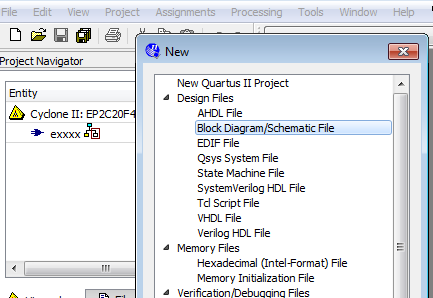
\includegraphics[width=\textwidth]{QuartusII1}
    \end{subfigure}
    ~
    \begin{subfigure}{0.3\textwidth}
        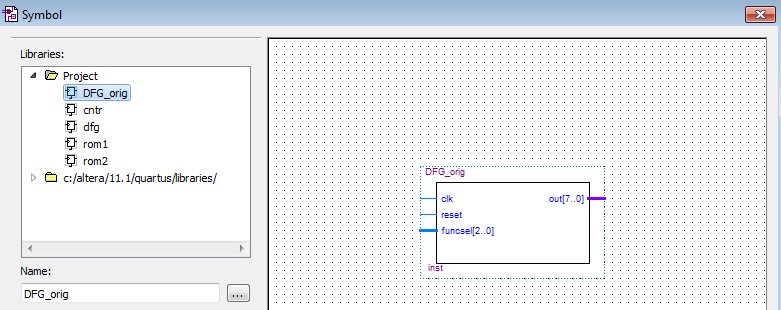
\includegraphics[width=\textwidth]{QuartusII2}
    \end{subfigure}
    ~
    \begin{subfigure}{0.3\textwidth}
        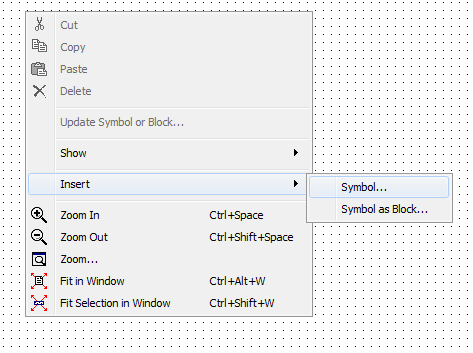
\includegraphics[width=\textwidth]{QuartusII3}
    \end{subfigure}
\end{figure}


You should use bus or line tool from the top toolbar menu 
\includegraphics[height=2ex]{QuartusII4} and make all the interconnects between components.

Double-click on the blank space in the Graphic Editor window, or click on the icon in the toolbar hat looks like an \texttt{AND} gate. A pop-up box will appear.

Expand the hierarchy in the Libraries box. First expand libraries, then expand the library primitives, followed by expanding the library logic comprises the logic gates. Use the gates if any is needed.

\begin{figure}
    \centering
    \caption{Block diagram in Quartus~II\label{fig:qblockdia}}
    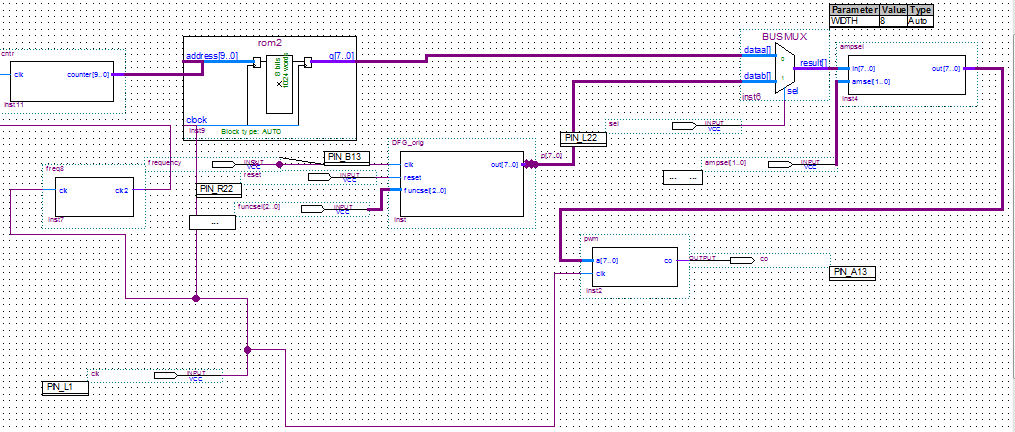
\includegraphics[width=\textwidth]{QuartusII5}
\end{figure}

When the schematic design is completed, compile it as before. Program the design on FPGA and record all the results.

\designverification{}

\section*{Pre-Lab Assignment}
\addcontentsline{toc}{section}{Pre-Lab Assignment}
Before coming to the lab, answer these questions. The pre-lab needs to be handed in at the start of the lab.

\begin{enumerate}
    \item Write a preliminary Verilog code for generating the rhomboid and the sine wave generation.
    \item Draw the datapath of the complete design, including all the input and output signals for each component and also any control signal that you used.
\end{enumerate}


\section*{Acknowledgment}
\addcontentsline{toc}{section}{Acknowledgment}

This lab manual was prepared and developed by \href{mailto:ktbasharkhah@gmail.com?subject=[DLDLab]\%20}{Katayoon Basharkhah}, PHD student of Digital Systems at University of Tehran, under the supervision of professor Zain Navabi.

This manual has been edited by \href{mailto:hadi.safari@ut.ac.ir?subject=[DLDLab]\%20}{Hadi Safari}, undergraduate student of Computer Engineering at University of Tehran.

\end{document}
